% ---------------------------------------------------------------------------
% Template simplificado para Dissertação/UFABC
% ---------------------------------------------------------------------------
\documentclass[
  12pt,
  openany,
  twoside,
  a4paper,
  english,
  brazil
]{abntex2}

% -----------------------------------------
% Pacotes OBRIGATÓRIOS
% -----------------------------------------
\usepackage{lmodern}      % Usa a fonte Latin Modern
\usepackage[T1]{fontenc}  % Codificação de fonte
\usepackage[utf8]{inputenc}    % Reconhece acentos
\usepackage{indentfirst}  % Indenta o primeiro parágrafo de cada seção
\usepackage{color}        % Controle de cores
\usepackage{graphicx}     % Inclusão de gráficos
\usepackage{epsfig,subfig}% Inclusão de figuras
\usepackage{lastpage}     % Usado na ficha catalográfica
\usepackage{microtype}    % Melhora a justificação

% -----------------------------------------
% Pacotes ADICIONAIS
% -----------------------------------------
\usepackage{float}
\usepackage{lipsum}                 % Texto de exemplo
\usepackage{amsmath,amssymb,mathrsfs} 
\usepackage{setspace}               % Espaçamento
\usepackage{verbatim}               % Ambiente "comment"
\usepackage{tabularx}               % Tabelas autoajustáveis
\usepackage{afterpage}              % Comandos após o fim da página
\usepackage{url}                    % Formatação de URLs
\usepackage{booktabs}               % Para linhas horizontais mais profissionais
\usepackage{longtable}              % Para tabelas longas
\usepackage{adjustbox}              % Para ajustar tabelas grandes

% -----------------------------------------
% Pacotes de CITAÇÕES (ABNT)
% -----------------------------------------
\usepackage[brazilian,hyperpageref]{backref}
\usepackage[alf]{abntex2cite}  % ou [num] se preferir citações numéricas

\usepackage{hyperref}
\pdfstringdefDisableCommands{%
  \def\uppercase#1{#1}%
}

% -----------------------------------------
% Configurações
% -----------------------------------------
% --- 
% CONFIGURAÇÕES DE PACOTES
% --- 

% ---
% Configurações do pacote backref
% Usado sem a opção hyperpageref de backref
\renewcommand{\backrefpagesname}{Citado na(s) página(s):~}
% Texto padrão antes do número das páginas
\renewcommand{\backref}{}
% Define os textos da citação
\renewcommand*{\backrefalt}[4]{
	\ifcase #1 %
		Nenhuma citação no texto.%
	\or
		Citado na página #2.%
	\else
		Citado #1 vezes nas páginas #2.%
	\fi}%
% ---  % Ajustes de citações
% ---
% Informações de dados para CAPA e FOLHA DE ROSTO
% ---
\titulo{Efeito da Neuromodulação Não Invasiva na Sincronicidade Cérebro-Corpo em Atletas do Basquetebol}
\autor{Danilo Cavalcante Brambila de Barros}
\local{São Bernardo do Campo - SP}
\data{2025}
\orientador{Prof. Dr. Alexandre Hideki Okano}
\coorientador{Prof. Dr. Edgard Morya}
\instituicao{%
  Universidade Federal do ABC - UFABC
  \par
  Centro de Matemática, Computação e Cognição 
  \par
  Programa de Pós-Graduação em Neurociência e Cognição}
\tipotrabalho{Dissertação (Mestrado)}
% O preambulo deve conter o tipo do trabalho, o objetivo,
% o nome da instituição e a área de concentração
\preambulo{\textbf{Dissertação de Mestrado} apresentada ao Programa de Pós-Graduação em Neurociência e Cognição, como parte dos requisitos necessários para a obtenção do Título de Mestre em Neurociência e Cognição.}
% ---          % Título, autor, orientador etc.
%  Configurações de aparência do PDF final
% NÃO ALTERAR!!!

% alterando o aspecto da cor azul
\definecolor{blue}{RGB}{41,5,195}

% informações do PDF
\makeatletter
\hypersetup{
     	%pagebackref=true,
		pdftitle={\@title}, 
		pdfauthor={\@author},
    	pdfsubject={\imprimirpreambulo},
	    pdfcreator={LaTeX with abnTeX2},
		pdfkeywords={abnt}{latex}{abntex}{abntex2}{trabalho acadêmico}, 
		colorlinks=true,       		% false: boxed links; true: colored links
    		linkcolor=blue,          	% color of internal links
    		citecolor=blue,        		% color of links to bibliography
    		filecolor=magenta,      		% color of file links
		urlcolor=blue,
		bookmarksdepth=4
} 
\makeatother
% ---        % Aparência do PDF final

\setlength{\parindent}{1.3cm}   % Tamanho da indentação
\setlength{\parskip}{0.2cm}     % Espaçamento entre parágrafos
\makeindex                       % Compilar índice remissivo

% Comando de gerar imagens, padronizando a width.
\newcommand{\standardfigure}[3]{
    \begin{figure}[htbp]
        \centering
        \includegraphics[width=0.7\textwidth]{#1}
        \caption{#2}
        \label{fig:#3}
    \end{figure}
}

\newcommand{\smallfigure}[3]{
  \begin{figure}[H]
  \centering
  \includegraphics[width=0.6\textwidth]{#1}
  \caption{\small #2}
  \label{#3}
  \end{figure}
}

\newcommand{\inputtable}[4]{%
    \begin{table}[htbp]
        \centering
        \caption{#2}
        \label{tab:#3}
        \begin{adjustbox}{width=\textwidth}
            \input{#1}
        \end{adjustbox}
        \vspace{0.5em}% <— espaço extra antes da fonte
        \source{#4}
    \end{table}
}

% -----------------------------------------

\begin{document}
% Remove espaço extra entre frases
\frenchspacing

% ----------------------------------------------------------
% ELEMENTOS PRÉ-TEXTUAIS
% ----------------------------------------------------------
\pretextual

% Capa
% ---
% Impressão da Capa
% ---
  \begin{capa}%
    \begin{figure}[h!]%
        \centering%
        
\includegraphics[scale=1.2]{figs/logo.png}%
      \end{figure}%
    \center
	\ABNTEXchapterfont\large{Universidade Federal do ABC \\ Centro de Matemática, Computação e Cognição \\ Programa de Pós-Graduação em Neurociência e Cognição}
	%\vspace{1.5cm}

    \vfill
    \ABNTEXchapterfont\bfseries\LARGE\imprimirtitulo
    \vfill

	%\vfill
	\ABNTEXchapterfont\large\imprimirautor
	\vfill
%
	Número de Ordem : XXXX
	
    \large\imprimirlocal, \large\imprimirdata

    \vspace*{1cm}
  \end{capa}
% ---

% Folha de rosto
\imprimirfolhaderosto*

% Ficha Catalográfica
% ---
% Ficha Catalográfica
% ---
% Exemplo de Ficha Catalográfica (Dados Internacionais de Catalogação).
% Se a biblioteca enviar um PDF oficial da ficha, basta:
%
% \begin{fichacatalografica}
%     \includepdf{fig_ficha_catalografica.pdf}
% \end{fichacatalografica}
%
% Caso contrário, use o modelo abaixo.
% ---
% Ficha Catalográfica
% ---

\begin{fichacatalografica}
    \vspace*{\fill}
    \hrule
    \begin{center}
    \begin{minipage}[c]{12cm}

    \imprimirautor

    \hspace{0.5cm} \imprimirtitulo /\\
    \hspace{0.5cm} \imprimirautor. -- \imprimirlocal, \imprimirdata.

    \hspace{0.5cm} \pageref{LastPage} p. : il. color. ; 30 cm.

    \hspace{0.5cm} \imprimirorientadorRotulo~\imprimirorientador

    \hspace{0.5cm}
    \parbox[t]{0.9\textwidth}{%
      \imprimirtipotrabalho~--~\imprimirinstituicao,
      \imprimirdata.
    }

    \hspace{0.5cm} Desenvolvido com apoio da Coordenação de Aperfeiçoamento de Pessoal de Nível Superior - Brasil (CAPES) - Código de Financiamento 001.

    \hspace{0.5cm}
    1. Neuromodulação. 2. Sincronização Cérebro-Corpo. 3. Basquetebol.\\
    I. Orientador. II. Universidade Federal do ABC. III. Programa de Pós-Graduação em Neurociência e Cognição. IV. Título.

    \hspace{8.75cm} CDU 02:141:005.7

    \end{minipage}
    \end{center}
    \hrule
\end{fichacatalografica}

% Folha de assinaturas
% ---
% Assinaturas
% ---
% Isto é um exemplo de Folha de aprovação, elemento obrigatório da NBR
% 14724/2011 (seção 4.2.1.3). Você pode utilizar este modelo até a aprovação
% do trabalho. Após isso, substitua todo o conteúdo deste arquivo por uma
% imagem da página assinada pela banca com o comando abaixo:
%
% \includepdf{folhadeaprovacao_final.pdf}
%
\begin{folhadeaprovacao}

  \begin{center}
    {\ABNTEXchapterfont\large\imprimirautor}

    \vspace*{\fill}\vspace*{\fill}
    \begin{center}
      \ABNTEXchapterfont\bfseries\Large\imprimirtitulo
    \end{center}
    \vspace*{\fill}
    
    \hspace{.45\textwidth}
    \begin{minipage}{.5\textwidth}
        \imprimirpreambulo
    \end{minipage}%
    \vspace*{\fill}
   \end{center}
        
 % Isso na versão final do trabalho!!!       
   Trabalho aprovado. \imprimirlocal, 01 de março de 2025:

   \assinatura{\textbf{\imprimirorientador} \\ Orientador} 
   \assinatura{\textbf{\imprimircoorientador} \\ Co-Orientador} 
   \assinatura{\textbf{Professor} \\ Convidado 1}
   \assinatura{\textbf{Professor} \\ Convidado 2}
   \assinatura{\textbf{Professor} \\ Convidado 3}
      
   \begin{center}
    \vspace*{0.5cm}
    {\large\imprimirlocal}
    \par
    {\large\imprimirdata}
    \vspace*{1cm}
  \end{center}
  
\end{folhadeaprovacao}
% ---

% Dedicatória
\begin{dedicatoria}
   \vspace*{\fill}
   \centering
   \noindent
   \textit{Dedico este trabalho a todos os estudantes e pesquisadores que, movidos pela curiosidade e pela paixão pelo conhecimento, buscam entender os mistérios do cérebro e do corpo humano. Que esta pesquisa possa servir como inspiração para novas descobertas e avanços na ciência.} \vspace*{\fill}
\end{dedicatoria}

% Agradecimentos
\chapter*{Agradecimentos}
\addcontentsline{toc}{chapter}{Agradecimentos}

Agradeço à minha \textbf{família}, pelo amor e apoio incondicional, fundamentais para eu chegar até aqui.  
Ao meu \textbf{orientador} e \textbf{coorientador}, pela oportunidade de explorar novas ideias, pelo incentivo contínuo e por ser fonte de inspiração e aprendizado ao longo desta caminhada.  
Aos \textbf{colegas de laboratório}, pela convivência, troca de ideias e colaboração, que tornaram essa jornada mais enriquecedora e inspiradora.  
Aos \textbf{professores e colaboradores} que, de alguma forma, contribuíram para a realização deste estudo.

\bigskip
\noindent

O presente trabalho foi realizado com apoio da Coordenação de Aperfeiçoamento de Pessoal de Nível Superior - Brasil (CAPES) - Código de Financiamento 001.

% Epígrafe
% ---
% Epígrafe
% ---
\begin{epigrafe}
    \vspace*{\fill}
	\begin{flushright}
		\textit{``Se o cérebro humano fosse simples o suficiente para que pudéssemos entendê-lo, seríamos tão simples que não conseguiríamos entendê-lo.''\\
		          (Emerson Pugh)}
	\end{flushright}
\end{epigrafe}
% ---

% Resumos (Resumo e Abstract)
% ---
% RESUMOS
% ---

% RESUMO em português
\setlength{\absparsep}{18pt} % ajusta o espaçamento dos parágrafos do resumo
\begin{resumo}
A sincronização entre oscilações neurais e ritmos fisiológicos, conceito central do \textit{Body-Brain Dynamic System} (BBDS), desempenha um papel fundamental na regulação e integração neural. Este estudo investigou os efeitos da neuromodulação catódica por estimulação transcraniana por corrente contínua de alta definição (\textit{High-Definition transcranial Direct Current Stimulation}, HD-tDCS), aplicada sobre o córtex pré-frontal dorsolateral (DLPFC) esquerdo, na sincronização cerebral em atletas de elite de basquetebol feminino em repouso (\textit{resting-state}). Utilizando um delineamento experimental cruzado e duplo-cego, com sessões ativa (catódica, 2 mA por 20 min) e simulada (\textit{sham}), analisou-se o acoplamento fásico intrafrequencial entre pares de canais de eletroencefalografia (EEG), bem como o acoplamento fásico \textit{cross-frequency} entre EEG e eletrocardiograma (ECG). Os índices utilizados foram o \textit{Phase Lag Index} (PLI) para conexões EEG-EEG na mesma banda de frequência e o \textit{Cross-Frequency Phase Linearity Measurement} (CF-PLM) para conexões EEG-ECG entre frequências distintas. Os resultados demonstraram que a neuromodulação catódica alterou significativamente os padrões de sincronização cerebral intrafrequencial e \textit{cross-frequency}, indicando efeito na modulação dos diversos acoplamentos EEG-EEG e EEG-ECG. Estes achados ressaltam o potencial da HD-tDCS como ferramenta para modulação direcionada da conectividade funcional cerebral e cardiovascular, com implicações tanto para contextos esportivos quanto clínicos.

\textbf{Palavras-chave}: Neuromodulação catódica. HD-tDCS. EEG. ECG. Conectividade funcional. Sincronização de fase. Atletas.

\end{resumo}


% ABSTRACT in english
\begin{resumo}[Abstract]
\begin{otherlanguage*}{english}
Synchronization between neural oscillations and physiological rhythms, a central concept of the Body-Brain Dynamic System (BBDS), plays a fundamental role in neural regulation and integration. This study investigated the effects of cathodal neuromodulation using High-Definition transcranial Direct Current Stimulation (HD-tDCS), applied over the left dorsolateral prefrontal cortex (DLPFC), on brain synchronization in elite female basketball athletes during resting-state. Employing a double-blind, crossover experimental design with active (cathodal, 2 mA for 20 min) and sham sessions, intra-frequency phase coupling between pairs of electroencephalography (EEG) channels, as well as cross-frequency phase coupling between EEG and electrocardiogram (ECG), were analyzed. The indices used were the Phase Lag Index (PLI) for EEG-EEG connections within the same frequency band and Cross-Frequency Phase Linearity Measurement (CF-PLM) for EEG-ECG connections across distinct frequencies. Results demonstrated that cathodal neuromodulation significantly altered intra-frequency and cross-frequency brain synchronization patterns, indicating modulatory effects on EEG-EEG and EEG-ECG couplings. These findings highlight the potential of HD-tDCS as a targeted tool for modulating functional brain and cardiovascular connectivity, with implications for both sports and clinical contexts.

\vspace{\onelineskip}
 
\noindent 
\textbf{Keywords}: Cathodal neuromodulation. HD-tDCS. EEG. ECG. Functional connectivity. Phase synchronization. Athletes.
\end{otherlanguage*}
\end{resumo}

% Lista de Figuras
\pdfbookmark[0]{\listfigurename}{lof}
\listoffigures*
\cleardoublepage

% Lista de Tabelas
\pdfbookmark[0]{\listtablename}{lot}
\listoftables*
\cleardoublepage

\begin{siglas}
  \item[BBDS] Sistema Dinâmico Corpo-Cérebro (\textit{Body Brain Dynamic System})
  \item[EEG] Eletroencefalografia (\textit{Electroencephalography})
  \item[EMG] Eletromiografia (\textit{Electromyography})
  \item[ECG] Eletrocardiograma (\textit{Electrocardiogram})
  \item[tDCS] Estimulação Transcraniana por Corrente Contínua (\textit{transcranial Direct Current Stimulation})
  \item[HD-tDCS] Estimulação Transcraniana por Corrente Contínua de Alta Definição (\textit{High-Definition transcranial Direct Current Stimulation})
  \item[tACS] Estimulação Transcraniana por Corrente Alternada (\textit{transcranial Alternating Current Stimulation})
  \item[rTMS] Estimulação Magnética Transcraniana Repetitiva (\textit{repetitive Transcranial Magnetic Stimulation})
  \item[DLPFC] Córtex Pré-frontal Dorsolateral (\textit{Dorsolateral Prefrontal Cortex})
  \item[mPFC] Córtex Pré-frontal Medial (\textit{Medial Prefrontal Cortex})
  \item[ASD] Transtorno do Espectro Autista (\textit{Autism Spectrum Disorder})
  \item[SAD] Transtorno de Ansiedade Social (\textit{Social Anxiety Disorder})
  \item[PLV] Valor de Bloqueio de Fase (\textit{Phase Locking Value})
  \item[PLI] Índice de Defasagem de Fase (\textit{Phase Lag Index})
  \item[CF-PLM] Medida de Linearidade de Fase Cross-Frequency (\textit{Cross-Frequency Phase Linearity Measurement})
  \item[SCAT] Teste de Ansiedade Competitiva no Esporte (\textit{Sport Competition Anxiety Test})
  \item[TQR] Escala de Qualidade Total de Recuperação (\textit{Total Quality Recovery})
  \item[PSE] Escala de Percepção Subjetiva de Esforço (\textit{Perceived Subjective Effort})
  \item[ICA] Análise de Componentes Independentes (\textit{Independent Component Analysis})
  \item[KDE] Estimativa de Densidade por Núcleo (\textit{Kernel Density Estimation})
  \item[ECOD] Detecção de Outliers Baseada na Distribuição Cumulativa Empírica (\textit{Empirical Cumulative Distribution-based Outlier Detection})
  \item[GPU] Unidade de Processamento Gráfico (\textit{Graphics Processing Unit})
  \item[BCa] Intervalos de Confiança Corrigidos e Acelerados (\textit{Bias-Corrected and Accelerated})
  \item[FDR-BH] Taxa de Falsas Descobertas-Benjamini-Hochberg (\textit{False Discovery Rate-Benjamini-Hochberg})
  \item[RBC] Correlação Biserial de Postos (\textit{Rank-Biserial Correlation})
  \item[IQR] Intervalo Interquartil (\textit{Interquartile Range})
\end{siglas}


\begin{simbolos}
  \item[$x(t)$] Sinal de entrada, função do tempo.
  \item[$y(t)$] Segundo sinal de entrada, função do tempo.
  \item[$x_{\mathrm{an}}(t)$] Representação analítica do sinal \(x(t)\), obtida pela Transformada de Hilbert.
  \item[$y_{\mathrm{an}}(t)$] Representação analítica do sinal \(y(t)\), obtida pela Transformada de Hilbert.
  \item[$\phi_x(t)$] Fase instantânea do sinal \(x(t)\).
  \item[$\phi_y(t)$] Fase instantânea do sinal \(y(t)\).
  \item[$\Delta \phi(t)$] Diferença de fase instantânea entre os sinais \(x(t)\) e \(y(t)\), definida por \(\Delta \phi(t) = \phi_x(t)-\phi_y(t)\).
  \item[$z(t)$] Sinal interferométrico, definido como 
  \[
  z(t)=\frac{x_{\mathrm{an}}(t)\, y_{\mathrm{an}}^*(t)}{\lvert x_{\mathrm{an}}(t)\rvert\, \lvert y_{\mathrm{an}}(t)\rvert} = e^{i\Delta \phi(t)}.
  \]
  \item[$SZ(f)$] Densidade espectral de potência (PSD) do sinal \(z(t)\), em função da frequência \(f\).
  \item[$f_\Delta$] Diferença entre as frequências centrais dos sinais envolvidos no acoplamento cross-frequency.
  \item[$B$] Largura de banda utilizada para integrar a PSD na definição do índice CF-PLM.
  \item[$\text{stat}$] Valor da estatística do teste \textit{Mann-Whitney U}.
  \item[$n_{\text{cathodic}}$] Número de observações (amostras) na condição catódica.
  \item[$n_{\text{sham}}$] Número de observações (amostras) na condição \textit{sham}.
\end{simbolos}


% Sumário
\pdfbookmark[0]{\contentsname}{toc}
\tableofcontents*
\cleardoublepage

% ----------------------------------------------------------
% ELEMENTOS TEXTUAIS
% ----------------------------------------------------------
\textual
\pagenumbering{arabic}
\setcounter{page}{1}

% ----------------------------------------------------------
% Capítulos
\part{Introdução e Fundamentação Teórica}
\chapter{Introdução}
\label{chap:introducao}

``puras''

"puras"

\textquotedblleft puras\textquotedblright

\enquote{puras}

\textquote{puras}

\emph{puras}

\textbf{puras}

\texttt{puras}



A neurociência tem avançado na compreensão da sincronização entre o cérebro e processos fisiológicos, destacando o papel das interações dinâmicas na integração entre sistemas corporais e neurais. Nesse contexto, o conceito de \textit{Body–Brain Dynamic System} (BBDS) tem ganhado espaço como uma abordagem para investigar como oscilações neurais se sincronizam com ritmos fisiológicos – como os da frequência cardíaca, respiratória e outros – modulando a atividade cerebral \cite{criscuolo2022cognition, cohen2017where}. Esse entendimento tem impulsionado o desenvolvimento de intervenções de neuromodulação capazes de modificar padrões rítmicos e, consequentemente, a função cerebral.

\section{Sincronicidade Cérebro-Corpo no Esporte}
O corpo humano possui uma capacidade intrínseca de sincronizar seus ritmos fisiológicos com estímulos ambientais e internos. Por exemplo, o ritmo respiratório pode alinhar-se a padrões de atividade sensorial e cognitiva \cite{haas1985effects}, e estados psicofisiológicos – como ansiedade, depressão e estresse – influenciam tanto a frequência cardíaca quanto a atividade neural \cite{criscuolo2022cognition}. Pesquisas recentes demonstram que a variabilidade dos ritmos cardíacos e respiratórios gera ciclos de alta e baixa excitabilidade, modulando a integração e a regulação neural. Estudos em neurocardiologia evidenciam que a interação entre mecanismos sensoriais (como barorreceptores e quimiorreceptores) e centros neurais superiores é essencial para a regulação dos padrões cardíacos \cite{marcondes2024linguagem}. Além disso, pesquisas com potenciais evocados pelo batimento cardíaco (HEPs) reforçam a importância da integração interoceptiva na formação da consciência corporal \cite{park2018neural, banelli2020skipping, mackinnon2013utilizing}.

Neste estudo, além de analisar a sincronização intrafrequencial entre pares de canais de EEG (EEG-EEG), investigamos a sincronicidade \textit{cross-frequency} entre sinais de EEG e ECG. Para isso, o sinal de ECG foi convertido em uma representação senoidal simples – baseada no pico R – que delimita de forma clara o ciclo cardíaco. Ao comparar, por exemplo, o canal Fp1 na banda alpha com esse sinal senoidal, é possível quantificar a sincronização entre a atividade cerebral e o ritmo cardíaco. Essa abordagem detalha o acoplamento entre oscilações cerebrais de diferentes frequências e o sinal cardíaco, contribuindo para a compreensão da interação entre os sistemas neural e cardiovascular, com especial relevância para intervenções neuromodulatórias em atletas. Ademais, modelos recentes exploram a previsibilidade dos sinais EEG alinhados com os batimentos cardíacos, ampliando o entendimento dos mecanismos de acoplamento entre a atividade neural e o ritmo cardíaco \cite{vergara2024exploring}.

\section{Neuromodulação e Modulação da Função Cerebral em Contextos Esportivos e Clínicos}
Para explorar os efeitos da neuromodulação na conectividade neural, este projeto investiga como a estimulação transcraniana por corrente contínua de alta definição (HD-tDCS), aplicada de forma catódica sobre o córtex pré-frontal dorsolateral (DLPFC) esquerdo, impacta os padrões de sincronização cerebral em atletas de elite de basquetebol feminino em repouso (\textit{resting state}). O delineamento experimental adotado é do tipo cruzado (cross-over) e duplo-cego, permitindo que os mesmos participantes sejam submetidos tanto à estimulação ativa quanto à condição controle (sham), reduzindo assim a influência de variáveis individuais e possibilitando uma análise mais precisa dos efeitos neuromodulatórios.

\subsection{Técnicas Convencionais de Neuromodulação}
A estimulação transcraniana por corrente contínua (tDCS) é uma técnica não invasiva que utiliza correntes elétricas fracas para modular a excitabilidade cortical e a atividade neuronal \cite{nitsche2000excitability, okano2013estimulacao, stagg2011physiological, purpura1965intracellular}. A aplicação de correntes anódicas geralmente aumenta a excitabilidade, enquanto a catódica a reduz. Para aumentar a focalidade da estimulação, foi desenvolvida a High-Definition tDCS (HD-tDCS), que utiliza arrays de eletrodos menores dispostos, por exemplo, na configuração \emph{4$\times$1} \cite{villamar2013hdtdcs}. Outras técnicas não invasivas – como tACS (estimulação transcraniana por corrente alternada) e rTMS (estimulação magnética transcraniana repetitiva) – também podem modificar a sincronização neural e a conectividade funcional, contribuindo para a modulação abrangente das redes cerebrais \cite{scheler2019neuromodulation, kunze2014high}.

\subsection{Aplicações Clínicas e Efeitos em Diferentes Contextos}
Estudos têm demonstrado o potencial das técnicas convencionais em contextos clínicos e esportivos:
\begin{itemize}
    \item Singh et al. \cite{singh2024evaluating} identificaram alterações na topologia da rede de EEG em repouso de pacientes com transtorno depressivo maior, sugerindo que a tDCS pode restaurar circuitos neurais disfuncionais.
    \item Toutant et al. \cite{toutant2024hdtdcs} demonstraram que a HD‑tDCS pode reorganizar o perfil espectral do EEG – com redução das frequências baixas (delta e theta) e aumento das frequências altas (beta e gamma) – em pacientes com epilepsia refratária.
    \item Čukić et al. \cite{cukic2018shift} relataram que a tDCS, dependendo da polaridade, provoca deslocamentos no estado energético do cérebro, refletidos em alterações do Mean State Shift (MSS) e da State Variance (SV).
    \item Dong et al. \cite{dong2023efficacy} evidenciaram que a estimulação não invasiva pode melhorar o estado de consciência em pacientes com transtornos do nível de consciência.
\end{itemize}

\subsection{Impacto nos Aspectos Emocionais, Interpessoais e na Reabilitação}
A neuromodulação influencia também aspectos emocionais, interpessoais e pode ser aplicada em processos de reabilitação:
\begin{itemize}
    \item Valenzuela et al. \cite{valenzuela2019enhancement} demonstraram que a tDCS pode melhorar o estado de humor em atletas.
    \item Estudos com tACS, como os de Rostami et al. \cite{rostami2020transcranial}, indicam que a estimulação a 6 Hz sobre o córtex pré-frontal medial melhora a atenção sustentada, modulando a sincronia alpha e theta.
    \item Spooner et al. \cite{spooner2020hdtdcs} mostraram que a HD-tDCS aplicada no DLPFC altera a conectividade na banda theta durante tarefas de atenção visual seletiva.
    \item Em contextos interpessoais, Long et al. \cite{long2023transcranial} relataram que a tDCS aplicada no lobo temporal anterior direito pode reduzir a sincronização neural interpessoal e os níveis de empatia emocional.
    \item No campo da reabilitação, Liu et al. \cite{liu2023effects} constataram que a tDCS diminui oscilações delta e aumenta oscilações alpha em pacientes pós-AVC, enquanto Han et al. \cite{han2022functional} observaram aumentos na conectividade funcional em pacientes com distúrbios de consciência após HD‑tDCS.
    \item Intervenções domiciliares com tDCS têm sido associadas ao aumento da sincronização neural em pacientes com depressão bipolar \cite{xiao2025enhanced}.
    \item Estudos com HD-tDCS aplicados no DLPFC sugerem que a estimulação pode alterar a conectividade parieto-frontal e a dinâmica dos circuitos neurais \cite{arif2021high}.
\end{itemize}

\subsection{Abordagens Multidimensionais, Modelos Matemáticos e Monitoramento Integrado}
Para ampliar o entendimento dos efeitos da neuromodulação, diversas abordagens têm sido empregadas:
\begin{itemize}
    \item Zhang et al. \cite{zhang2022multidimensional} realizaram uma avaliação abrangente das métricas de EEG em intervenções neuromodulatórias.
    \item Jones et al. \cite{jones2017frontoparietal} demonstraram que a combinação de tDCS com treinamento de memória de trabalho aumenta a sincronia em redes fronto-parietais.
    \item Estudos com tDCS bilateral indicam que há remodelação das redes cerebrais em repouso, sugerindo indução de plasticidade em regiões não diretamente estimuladas \cite{pellegrino2018bilateral}.
    \item Modelos matemáticos, como o proposto por Riedinger e Hutt \cite{riedinger2022model}, explicam como a tDCS modula a excitabilidade cerebral e a potência do EEG.
    \item Abordagens de controle em loop fechado para oscilações gamma, exploradas por Zhang et al. \cite{zhang2024closed}, indicam que intervenções transcranianas – tanto por tDCS quanto por rTMS – podem aumentar as oscilações gamma.
    \item Análises de grafos aplicadas à tDCS revelam alterações na sincronização cortical que dependem da polaridade da estimulação \cite{mancini2016assessing, pellegrino2019transcranial, schollmann2019anodal}.
    \item Por fim, a viabilidade do monitoramento simultâneo de EEG durante a tDCS foi demonstrada por Schestatsky et al. \cite{schesatsky2013simultaneous}, facilitando a avaliação contínua da excitabilidade cortical.
\end{itemize}

\subsection{Abordagens Alternativas e Complementares}
Diversas técnicas alternativas de neuromodulação vêm sendo exploradas para ajustar a sincronização neural e ampliar o entendimento dos mecanismos moduladores:
\begin{itemize}
    \item Estudos de Boecker et al. \cite{boecker2024interpersonal} investigaram a sincronia neural interpessoal, demonstrando que intervenções envolvendo estimulação cerebral combinada com neurofeedback podem aprimorar a coordenação dos sinais durante interações sociais, especialmente em populações com transtorno do espectro autista (ASD), transtorno de ansiedade social (SAD) e condições correlatas.
    \item Revisões de McNaughton and Redcay \cite{mcnaughton2020interpersonal} e Baldwin et al. \cite{baldwin2014evidence} apontam que indivíduos com ASD frequentemente exibem comportamentos temporalmente assíncronos em tarefas de integração sensorial, sugerindo o potencial de intervenções neuromodulatórias alternativas para restabelecer a sincronização funcional.
    \item Estudos adicionais \cite{gerloff2022autism, quinones2021dysfunction, key2022greater, tanabe2012hard} corroboram a hipótese de que a desincronia interpessoal pode estar associada a déficits em múltiplos níveis, sugerindo que abordagens complementares podem ser essenciais para restabelecer a comunicação neural.
    \item No campo do neurofeedback, evidências sugerem que essa abordagem pode reduzir sintomas de ansiedade generalizada e fobias específicas \cite{hou2021neurofeedback, zilverstand2015fmri}. Investigações utilizando neurofeedback baseado em NIRS demonstraram a viabilidade de treinar o controle do DLPFC em indivíduos com ansiedade social \cite{kimmig2019feasibility, direito2021training, steiner2014pilot, lamarca2018facilitating, catala2017treatment}, com análises econômicas indicando que os custos podem ser compatíveis com outras intervenções terapêuticas \cite{arnold2013eeg}.
    \item Em termos de potencialização de oscilações, Maiella et al. \cite{maiella2022simultaneous} exploraram a combinação de tACS e TMS para aumentar as oscilações gamma no DLPFC. De modo complementar, Zrenner et al. \cite{zrenner2020brain} demonstraram a eficácia da rTMS sincronizada com oscilações alpha no DLPFC para pacientes com depressão resistente, e Konrad et al. \cite{konrad2024interpersonal} discutiram intervenções voltadas à sincronia neural interpessoal como uma via inovadora para tratamentos clínicos.
\end{itemize}

\section{Medidas Neurofisiológicas}
Para compreender a complexa interação entre o cérebro e o corpo, é possível integrar diversas técnicas que permitam registrar simultaneamente a atividade elétrica cerebral e sinais fisiológicos. A eletroencefalografia (EEG) fornece dados sobre a atividade neural, possibilitando a extração de oscilações que podem ser decompostas nas bandas clássicas – delta, theta, alpha, beta e gamma – cada uma associada a escalas temporais e funções cognitivas ou comportamentais específicas \cite{cohen2017where, bullmore2009complex}.

Além do EEG, técnicas como a eletromiografia (EMG) e o eletrocardiograma (ECG) são empregadas para monitorar a atividade muscular e os ritmos cardíacos, respectivamente. Em determinadas situações, a posição estratégica dos eletrodos de EMG pode possibilitar a detecção dos picos dos batimentos cardíacos – refletindo a despolarização – quando o ECG tradicional não está disponível ou quando se busca uma integração mais próxima com outros sinais fisiológicos. Essa abordagem permite, por exemplo, capturar a dinâmica do ciclo cardíaco a partir da atividade do músculo peitoral maior, conforme realizado neste estudo.

Esses registros permitem analisar o acoplamento de frequências cruzadas (\textit{cross-frequency coupling}, CFC), fenômeno no qual oscilações de diferentes frequências interagem entre si. O CFC possibilita compreender melhor processos de integração neural e corporal, como evidenciado em estudos que investigam a modulação da cognição e desempenho esportivo por meio da interação entre bandas rápidas (por exemplo, gamma) e lentas (como theta) \cite{criscuolo2022cognition, cohen2017where}. A análise desse fenômeno fundamenta estratégias para a otimização do desempenho esportivo, neuromodulação e reabilitação neurológica.

\part{Objetivos e Hipóteses}
\chapter{Objetivos}
\label{chap:objetivos}

Este estudo tem como objetivo investigar os efeitos da estimulação transcraniana por corrente contínua de alta definição (HD-tDCS), aplicada de forma catódica sobre o córtex pré-frontal dorsolateral esquerdo (DLPFC esquerdo), na conectividade funcional em atletas de elite do basquetebol feminino durante o repouso (\textit{resting-state}). A conectividade será analisada entre sinais de EEG dentro da mesma banda de frequência (delta, theta, alpha, beta e gamma), bem como entre sinais EEG (nas mesmas bandas citadas) e ECG, em uma abordagem \textit{cross-frequency}, já que o ECG possui uma frequência intrínseca única correspondente ao ciclo cardíaco. Para tal, serão empregadas técnicas de análise de sincronicidade, especificamente o \textit{Phase Lag Index} (PLI), para conectividade EEG-EEG intrafrequencial, e o \textit{Cross-Frequency Phase Linearity Measurement} (CF-PLM), para conectividade EEG-ECG. As análises serão realizadas comparando os períodos pré e pós-estimulação, nas condições sham (controle) e catódica.
\chapter{Hipóteses}
\label{chap:hipoteses}

A hipótese central deste estudo é que a aplicação de HD-tDCS modula significativamente a sincronicidade entre os sinais de EEG e ECG, alterando tanto a direção quanto a intensidade do acoplamento entre os sistemas cerebral e cardíaco. Especificamente, espera-se que a HD-tDCS reconfigure a conectividade funcional ao promover um aumento da sincronização em bandas de frequência relevantes.

\part{Metodologia e Processamento}
\chapter{Metodologia}
\label{chap:metodologia}

Este estudo utiliza dados previamente coletados de atletas profissionais de basquetebol feminino em repouso, abrangendo medidas de eletroencefalografia (EEG) e eletromiografia (EMG). O objetivo principal é investigar a sincronicidade entre sinais neurofisiológicos e musculares e avaliar como a estimulação transcraniana por corrente contínua de alta definição (HD-tDCS) catódica, aplicada sobre o córtex pré-frontal dorsolateral esquerdo, pode modular a atividade neural em condições de repouso, fornecendo insights sobre potenciais efeitos neuromodulatórios em atletas

\section{Participantes e Coleta de Dados}

O estudo foi aprovado pelo Comitê de Ética em Pesquisa da UFABC (protocolo: 08070819.1.0000.5594) e conduzido em conformidade com os princípios éticos estabelecidos pela Declaração de Helsinque para experimentos envolvendo seres humanos. Todas as participantes assinaram o Termo de Consentimento Livre e Esclarecido (TCLE) antes do início da coleta de dados.

Foram selecionadas atletas de elite, caracterizadas por:
\begin{itemize}
    \item Participação regular no programa de treinamento da equipe;
    \item Regime de treinamento superior a 10 horas semanais;
    \item Ausência de doenças ou lesões que pudessem interferir na execução do protocolo.
\end{itemize}

A amostra foi detalhadamente caracterizada por meio da mensuração de parâmetros como massa corporal e estatura, além da coleta de informações pessoais e esportivas (nome, data de nascimento, categoria, experiência esportiva, posição no time, fase da temporada, membro dominante e estilo de arremesso). Devido a problemas técnicos durante a coleta, apenas os dados de 6 atletas foram incluídos nas análises. O número de sujeitos reflete não apenas a disponibilidade das participantes, mas também a especificidade do grupo estudado – atletas de basquetebol feminino de elite da mesma equipe – e a complexidade dos protocolos, que exigem múltiplas visitas ao laboratório e a sincronização de diversos equipamentos.

\section{Delineamento Experimental}

O estudo utilizou um delineamento experimental randomizado, cruzado e duplo-cego. Cada participante foi submetida às condições catódica (HD-tDCS) e sham em momentos distintos, e a análise foi realizada considerando os pares de canais de forma agrupada.

Antes do início das sessões experimentais, foi realizada uma sessão de familiarização na qual as atletas receberam informações detalhadas sobre os objetivos, procedimentos, riscos e benefícios do estudo, além de treinamento prático para se familiarizarem com o protocolo e os equipamentos utilizados.

\standardfigure{figs/0_intro_e_desenho_experimental/desenho_experimental_drawio.png}
{Fluxo do protocolo experimental, incluindo a sessão de familiarização, as duas sessões experimentais (com estimulação catódica ou sham), as coletas de EEG/ECG em repouso e a execução de 100 arremessos pré-estimulação e 100 arremessos pós-estimulação por sessão.}
{desenho_experimental}

As sessões experimentais seguiram a seguinte estrutura:
\begin{itemize}
    \item \textbf{Sessão 1:} Familiarização com os dispositivos e procedimentos do estudo.
    \item \textbf{Sessões 2 e 3:} Execução do protocolo experimental, na qual cada atleta realizou 100 arremessos pré-estimulação e 100 arremessos pós-estimulação, totalizando 200 arremessos por sessão (ou 400 no total).
\end{itemize}


Para garantir a padronização das condições experimentais, todas as sessões foram realizadas no mesmo local e horário habitual de treinamento das atletas, sob condições controladas de iluminação, temperatura e ruído. A ordem das condições (HD-tDCS ativa e sham) foi definida aleatoriamente para cada participante por meio de um gerador de números aleatórios, assegurando imparcialidade no delineamento cruzado. Antes de cada sessão, os equipamentos de EEG e ECG foram calibrados e tiveram suas impedâncias verificadas, garantindo a qualidade dos registros. As participantes foram continuamente monitoradas quanto a possíveis efeitos adversos ou desconfortos decorrentes da estimulação, e os dados foram armazenados digitalmente com protocolos rigorosos de backup e verificação de integridade, assegurando sua reprodutibilidade e confiabilidade para as análises subsequentes.

\section{Questionários e Escalas}

Durante a coleta dos dados experimentais, foram aplicados questionários e escalas com o intuito de avaliar aspectos subjetivos relacionados ao estado psicológico e fisiológico das atletas. Embora esses instrumentos tenham sido incluídos no protocolo inicial com a finalidade de fornecer uma visão complementar às medidas neurofisiológicas, os dados obtidos não foram utilizados nas análises estatísticas ou nos resultados apresentados neste estudo. Os instrumentos aplicados foram:

\begin{itemize}
    \item \textbf{Escala de Qualidade Total de Recuperação (TQR):} Avalia a percepção subjetiva do estado geral de recuperação física e mental após as sessões experimentais.
    \item \textbf{Escala de Percepção Subjetiva de Esforço (PSE):} Mensura o esforço percebido pelas participantes durante as sessões experimentais.
    \item \textbf{Sport Competition Anxiety Test (SCAT):} Identifica níveis de ansiedade competitiva das participantes.
    \item \textbf{Questionário de Motivação Relacionado ao Exercício:} Investiga os fatores motivacionais das participantes durante o período experimental.
\end{itemize}

Dessa forma, apesar de terem sido coletados, os dados desses questionários não são apresentados nem discutidos, dado o escopo específico das análises neurofisiológicas deste trabalho.

\subsection{Protocolo de HD-tDCS}
\label{subsec:hdtdcs_protocol}

A estimulação transcraniana por corrente contínua de alta definição (HD-tDCS) foi aplicada com um estimulador digital MxN da Soterix Medical, utilizando eletrodos de Ag/AgCl integrados a uma touca de EEG. Diferentemente da configuração clássica 4$\times$1 descrita em Villamar et al. \cite{villamar2013hdtdcs}, optou-se por um arranjo customizado, em que o posicionamento dos eletrodos foi determinado por modelagem computacional, visando otimizar a focalidade da corrente no córtex pré-frontal dorsolateral (DLPFC) esquerdo.

Nesta montagem, um eletrodo principal foi posicionado sobre o DLPFC, enquanto eletrodos de retorno foram distribuídos de forma a contornar a região-alvo, garantindo uma distribuição concentrada da corrente. Foram aplicadas duas condições experimentais:
\begin{itemize}
    \item \textbf{Estimulação Catódica (Ativa):} Corrente contínua de 2\,mA aplicada por 20 minutos.
    \item \textbf{Condição Sham (Simulada):} A corrente foi interrompida após os 30\,segundos iniciais, de modo a reproduzir a sensação inicial sem promover a modulação cortical efetiva.
\end{itemize}

A calibração do dispositivo e a verificação da impedância (mantida abaixo de 5\,k$\Omega$) foram realizadas antes de cada sessão, assegurando a qualidade e a confiabilidade dos dados registrados. Essa abordagem, fundamentada em parâmetros estabelecidos na literatura \cite{datta2008transcranial, stagg2011physiological}, permitiu uma estimulação focalizada e segura, adequada ao delineamento experimental adotado no presente estudo.


\subsection{Processamento e Análise de Dados}

O processamento e a análise dos dados seguiram um fluxo estruturado que abrange desde a coleta e organização dos arquivos até a extração das métricas de sincronização e a aplicação de testes estatísticos para avaliar as diferenças entre as condições experimentais. A Figura~\ref{fig:fluxo_processamento} apresenta um diagrama geral dessas etapas.

\standardfigure{figs/0_intro_e_desenho_experimental/diagrama_processamento_e_analise_drawio.png}
{Fluxo geral de processamento e análise de dados, desde a coleta e organização dos arquivos, passando pelas etapas de pré-processamento (EEG e ECG), sincronização temporal, extração de métricas de sincronização (PLI, PLV e CF-PLM) e, por fim, análises estatísticas e de conectividade em rede.}
{fluxo_processamento}


\subsubsection{Pré-processamento de Dados}
Os sinais de EEG e EMG foram submetidos a etapas de pré-processamento que incluíram a filtragem de ruídos e a remoção de artefatos por meio de Independent Component Analysis (ICA). Paralelamente, os sinais de ECG passaram por processos de detecção de picos e extração do ciclo cardíaco, garantindo assim a qualidade e a consistência dos dados analisados.

\subsubsection{Sincronização de Sinais}
Para possibilitar uma análise integrada, os sinais de EEG e ECG foram alinhados temporalmente, assegurando que as medidas extraídas estivessem sincronizadas e pudessem ser comparadas corretamente.

\subsubsection{Cálculo de Sincronização Funcional}
A sincronização entre os sinais foi avaliada utilizando três métricas. O Phase Locking Value (PLV) e o Phase Lag Index (PLI) foram aplicados para quantificar a conectividade na mesma faixa de frequência, enquanto a Cross-Frequency Phase Linearity Measurement (CF-PLM) foi empregada para avaliar o acoplamento entre frequências distintas. Antes de sua aplicação nos dados experimentais, esses métodos foram testados e validados utilizando sinais simulados.

\subsubsection{Análise Estatística} Para investigar as diferenças entre as condições experimentais, aplicamos métodos estatísticos robustos, incluindo testes de normalidade, testes não paramétricos e correções para comparações múltiplas. Adicionalmente, foram utilizadas medidas de centralidade em redes para avaliar a conectividade funcional entre diferentes regiões corticais. Os padrões de conectividade foram representados por meio de gráficos e redes, facilitando a visualização e a interpretação dos resultados.

Esse fluxo sistemático permitiu uma abordagem rigorosa para explorar a sincronicidade cerebral e avaliar o impacto da estimulação transcraniana na conectividade neural das atletas em estado de repouso.

\chapter{Pré-processamento de Dados}
\label{chap:preprocessamento_de_dados}

\section{Preparação dos Dados}

Os dados utilizados neste estudo foram coletados em sessões experimentais com atletas profissionais de basquetebol feminino, submetidas a condições de estimulação transcraniana por corrente contínua de alta definição (HD-tDCS) e a uma condição de controle (sham). Neste capítulo, descrevemos os procedimentos realizados para organizar, sincronizar e preparar os sinais de eletroencefalografia (EEG) e eletrocardiografia (ECG) para análise.

\subsection{Organização Inicial dos Dados}

Os dados de EEG e ECG foram armazenados em arquivos separados, correspondentes a cada atleta e condição experimental (\textit{pre\_sham}, \textit{post\_sham}, \textit{pre\_cathodic}, \textit{post\_cathodic}). Os sinais de EEG foram originalmente registrados a 1000 Hz, enquanto os sinais de ECG – obtidos a partir do EMG do músculo peitoral maior – foram registrados a 1111,11 Hz. Nesta etapa, os arquivos foram:
\begin{itemize}
    \item Identificados e associados a cada atleta e condição;
    \item Renomeados e normalizados para garantir consistência;
    \item Submetidos a uma verificação de integridade para evitar erros no processamento.
\end{itemize}

\subsection{Sincronização Temporal entre EEG e ECG}

Devido ao início não sincronizado das gravações, foi necessário alinhar temporalmente os sinais de EEG e ECG. Com base em marcadores do período baseline, os seguintes passos foram realizados:
\begin{itemize}
    \item Extração dos tempos de início e fim do baseline para cada modalidade;
    \item Remoção dos primeiros e últimos 15 segundos de cada gravação, minimizando artefatos de borda;
    \item Ajuste dos timestamps para que os sinais iniciassem simultaneamente;
\end{itemize}

\subsection{Estruturação dos Dados}

Após a sincronização, os dados foram organizados para o processamento subsequente. Os sinais de EEG foram armazenados em formato FIF, preservando as informações dos canais e os metadados, enquanto os dados de ECG foram exportados em formato CSV.


\section{Pré-processamento dos Sinais}

Esta seção descreve os procedimentos aplicados para garantir a qualidade dos sinais, incluindo filtragem, remoção de artefatos e segmentação.

\subsection{Pré-processamento do EEG}

\subsubsection{Filtragem, Reamostragem e Preparação dos Dados de EEG}

O processamento dos dados de EEG envolveu as seguintes etapas:
\begin{itemize}
    \item \textbf{Aquisição e Carregamento:} Os dados brutos foram baixados do Google Drive e carregados via MNE-Python a partir de arquivos exportados do software BrainVision (ou, alternativamente, em formato EEGLAB). Após o carregamento, os canais foram renomeados conforme uma convenção padronizada (por exemplo, Fp1, Fz, F3, etc.) e canais irrelevantes foram removidos. (Ver Figura~\ref{fig:exemplo_sinais_eeg})
    \item \textbf{Aplicação de Montage:} Foi aplicado o montage padrão \textit{standard\_1005} para assegurar a correta localização dos eletrodos, conforme ilustrado no diagrama do sistema 10-20. (Ver Figura~\ref{fig:sistema_10_20})
    \item \textbf{Definição do Período de Análise:} Com base nas informações extraídas dos arquivos de baseline, os dados foram recortados para um intervalo que excluiu os primeiros e últimos 15 segundos da gravação, reduzindo artefatos de borda.
    \item \textbf{Filtragem:} Aplicou-se um filtro passa-banda entre 0,5 e 60 Hz para eliminar ruídos fora do intervalo de interesse, seguido de um filtro notch em 60 Hz para remover interferências da rede elétrica.
    \item \textbf{Reamostragem:} Para padronizar a taxa de amostragem e facilitar o alinhamento com outros sinais (como o ECG), os dados de EEG foram reamostrados para 500 Hz.
\end{itemize}

\begin{figure}[htb]
    \centering
    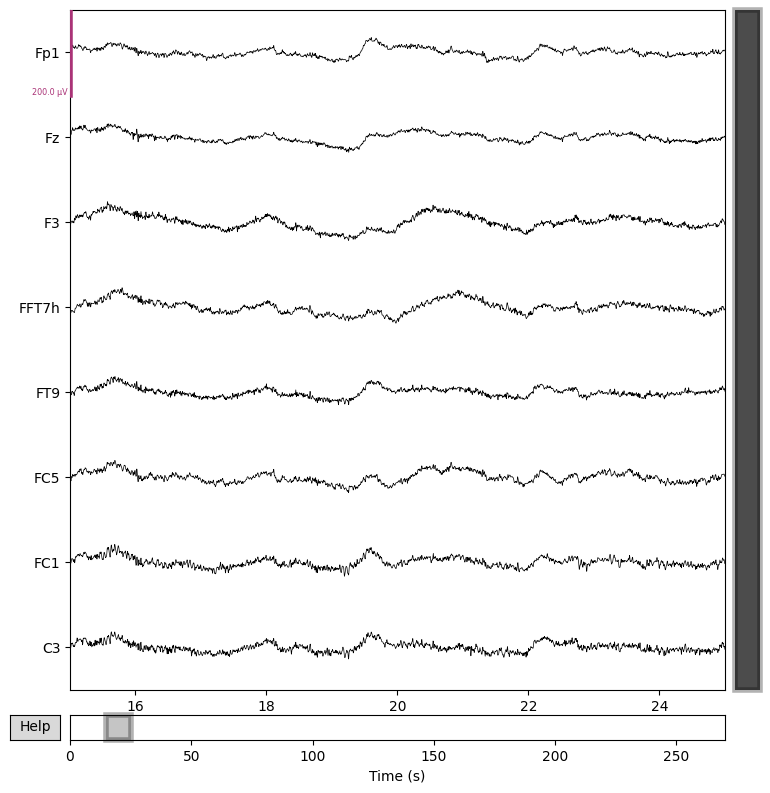
\includegraphics[width=0.8\textwidth]{figs/1_preprocessamento_eeg/2_exemplo_sinais_canais_eeg.png}
    \caption{Exemplo de sinais brutos de EEG, ilustrando a variação natural dos canais ao longo do tempo.}
    \label{fig:exemplo_sinais_eeg}
\end{figure}

\begin{figure}[htb]
    \centering
    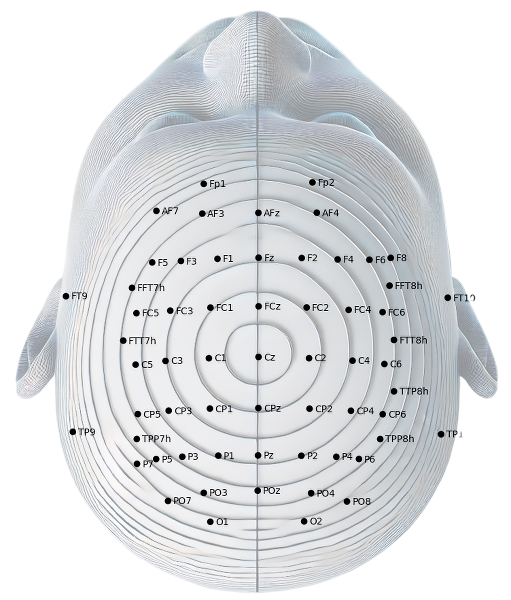
\includegraphics[width=0.8\textwidth]{figs/1_preprocessamento_eeg/1_sistema_10_20.png}
    \caption{Diagrama do sistema 10-20, demonstrando a localização padronizada dos eletrodos no couro cabeludo.}
    \label{fig:sistema_10_20}
\end{figure}

\subsubsection{Limpeza de Artefatos e Remoção de Componentes de Ruído (ICA)}

Para aprimorar a qualidade dos sinais de EEG, foi empregada a Análise de Componentes Independentes (ICA) conforme as seguintes etapas:
\begin{itemize}
    \item \textbf{Definição dos Componentes:} O número de componentes foi definido igual ao número de canais bons disponíveis (excluindo os canais previamente identificados como ruins por inspeção visual).
    \item \textbf{Aplicação do ICA:} Utilizou-se o método FastICA para decompor o sinal, preservando as informações críticas para a análise de sincronicidade.
    \item \textbf{Estimativa de Parâmetros de Rejeição:} A biblioteca \textit{autoreject} foi empregada para determinar, através de épocas de duração fixa, os limites ideais para rejeição de artefatos.
    \item \textbf{Identificação Automática de Artefatos:} Componentes relacionados a artefatos oculares (usando canais como Fp1 e Fp2) e à atividade cardíaca foram identificados automaticamente. Adicionalmente, uma análise baseada na curtose foi realizada para detectar componentes com alta amplitude, indicativos de artefatos.
    \item \textbf{Inspeção Visual e Seleção:} Foram gerados gráficos das propriedades dos componentes e uma visualização interativa, inclusive com animação GIF, que permitiram a inspeção manual dos componentes para decidir quais excluir. (Ver Figuras~\ref{fig:componentes_pos_ICA})
    \item \textbf{Aplicação e Salvamento:} Após a definição dos componentes a serem removidos, o ICA foi aplicado para eliminar os artefatos identificados, gerando um sinal de EEG limpo, que foi salvo em formato FIF para futuras análises.
\end{itemize}

\begin{figure}[htb]
    \centering
    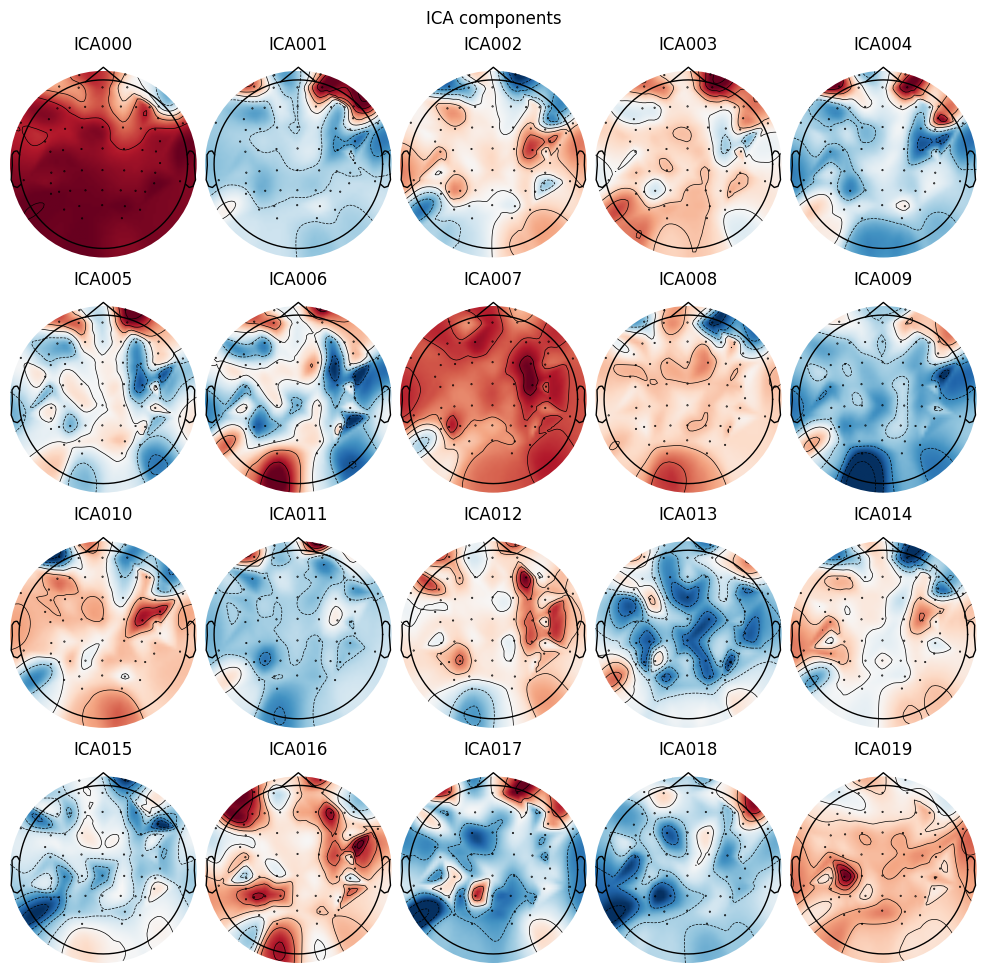
\includegraphics[width=0.8\textwidth]{figs/1_preprocessamento_eeg/3_exemplo_compomentes_pos_ICA.png}
    \caption{Exemplo de componentes obtidos após a aplicação do ICA, com mapas topográficos que evidenciam a distribuição espacial de cada componente.}
    \label{fig:componentes_pos_ICA}
\end{figure}

\begin{figure}[htb]
    \centering
    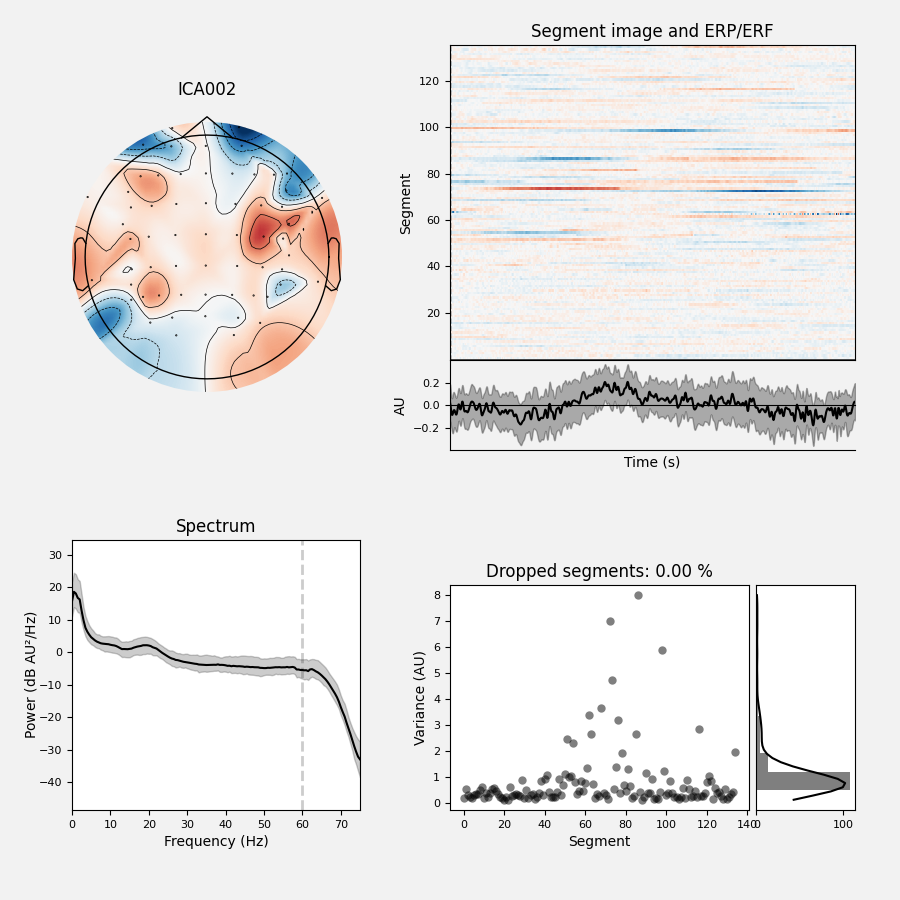
\includegraphics[width=0.8\textwidth]{figs/1_preprocessamento_eeg/4_exemplo_ICA_component_analysis.png}
    \caption{Exemplo de análise detalhada de um componente ICA, apresentando o mapa topográfico, o espectro de frequência e outras características relevantes para a identificação de artefatos.}
    \label{fig:exemplo_ICA_component_analysis}
\end{figure}


\subsection{Pré-processamento do Sinal de ECG}
\label{subsec:preprocess_ecg}

O processamento do sinal de ECG foi realizado com o objetivo de obter uma versão limpa e refinada do sinal, que permitisse a detecção precisa dos R-peaks e a extração de informações de fase. As etapas foram organizadas da seguinte forma:

\subsubsection{Aquisição e Segmentação dos Dados de ECG}

\begin{itemize}
    \item \textbf{Aquisição:} Os dados de ECG foram coletados juntamente com informações sobre os tempos de início e fim do período de baseline para cada condição experimental, garantindo a correta identificação dos intervalos de interesse para análise.
    \item \textbf{Segmentação:} Com base nos tempos extraídos dos arquivos de baseline, o sinal bruto foi segmentado para selecionar apenas o intervalo correspondente à condição de interesse. Para reduzir artefatos nas bordas, os primeiros e últimos 15 segundos foram removidos.
\end{itemize}

\subsubsection{Limpeza do Sinal e Detecção de Picos}

\begin{itemize}
    \item \textbf{Limpeza:} Utilizou-se a biblioteca NeuroKit2 para processar o sinal segmentado e remover ruídos, gerando uma versão limpa do ECG.
    
    \item \textbf{Detecção Automática de Picos:} Foi aplicado um algoritmo para detecção automática dos picos R (R-peaks) no sinal limpo, identificando os batimentos cardíacos. A Figura~\ref{fig:ecg_picos_detectados} ilustra um exemplo em que o sinal bruto (cinza) é sobreposto ao sinal limpo (azul), enquanto os picos R são marcados em vermelho.
    
    \item \textbf{Correção Manual dos Picos R:} Após a detecção automática, foi realizada uma inspeção visual cuidadosa utilizando gráficos interativos para identificar:
    \begin{itemize}
        \item Ausência de picos em locais onde deveriam ocorrer, com inserção manual dos picos faltantes por meio da identificação precisa dos timestamps correspondentes.
        \item Presença de picos falsos em regiões sem batimentos válidos, com remoção manual desses picos com base nos timestamps detectados como incorretos.
    \end{itemize}
    Esse ajuste garante a acurácia na identificação dos batimentos cardíacos, evitando tanto a omissão quanto a inclusão indevida de eventos.
\end{itemize}

\begin{figure}[htb]
    \centering
    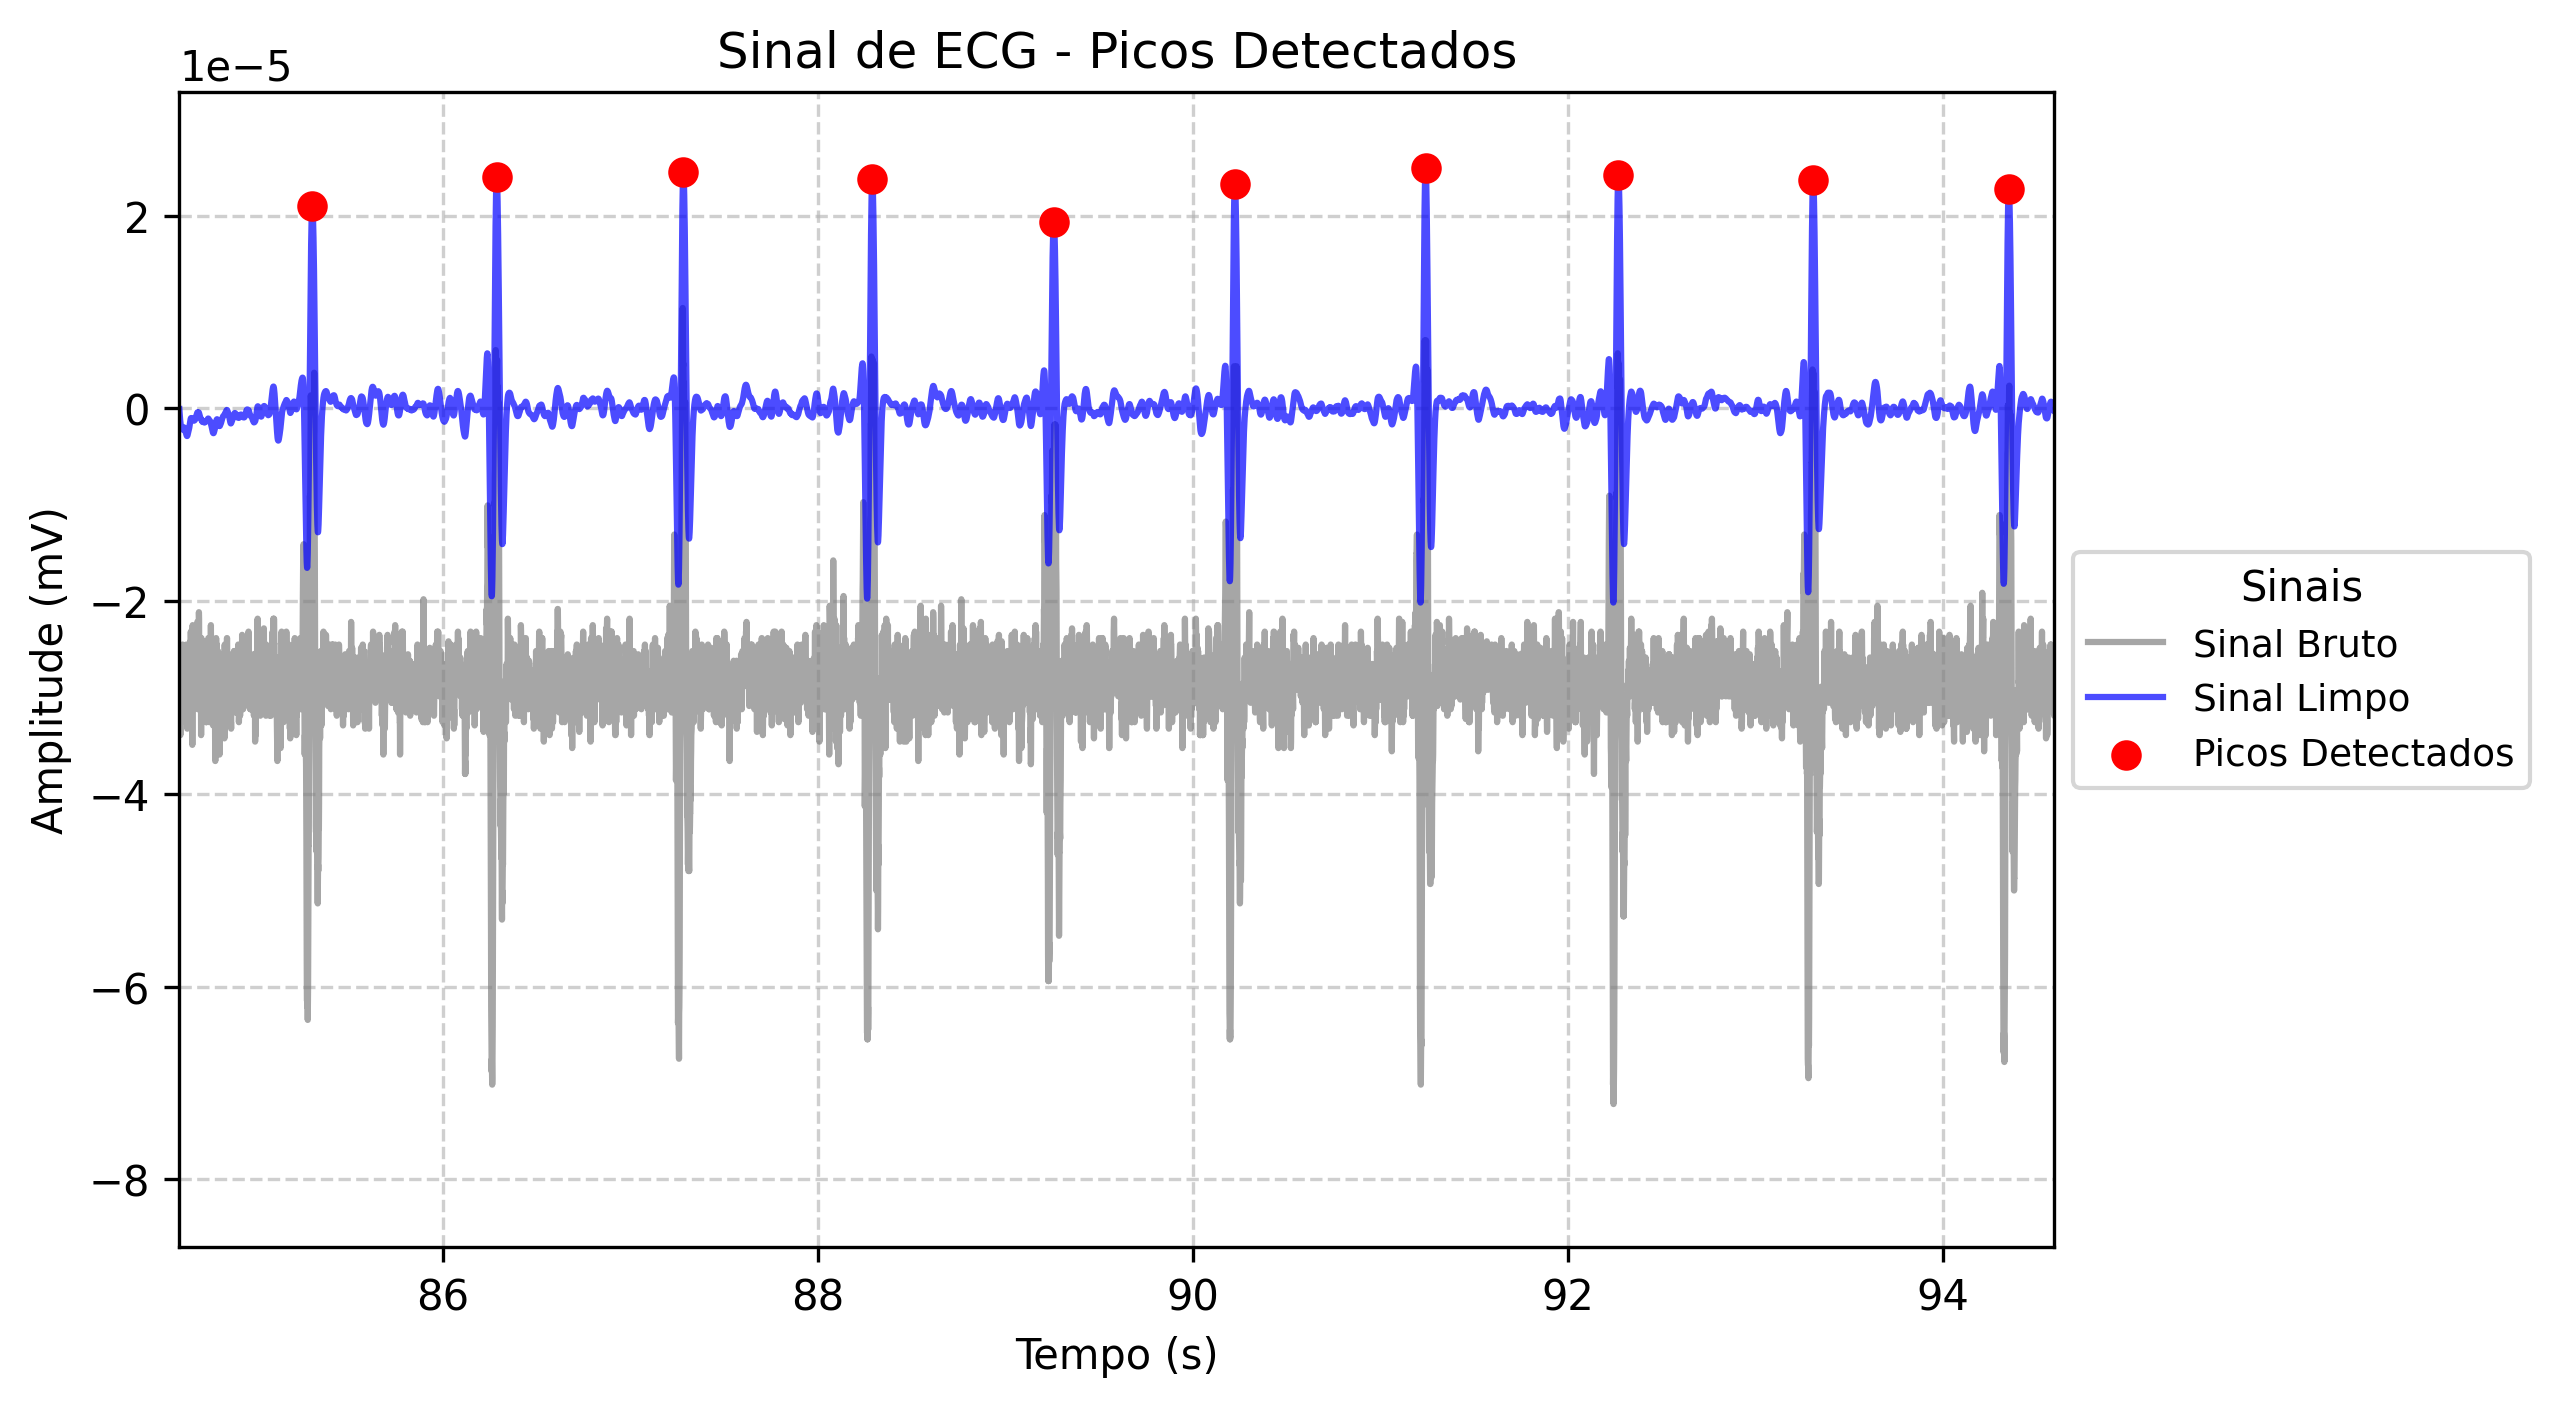
\includegraphics[width=0.8\textwidth]{figs/2_preprocessamento_ecg/1_Sinal_de_ECG_-_Picos_Detectados_zoom.png}
    \caption{Exemplo de sinal de ECG com picos detectados. O sinal bruto (cinza) é sobreposto pelo sinal limpo (azul), enquanto os picos R são marcados em vermelho.}
    \label{fig:ecg_picos_detectados}
\end{figure}

\subsubsection{Aplicação de Filtros Complementares}

Para refinar a definição dos eventos do ECG, foram aplicados filtros adicionais:
\begin{itemize}
    \item \textbf{Filtro de Janela:} Extração de uma janela de \(\pm50\) ms ao redor de cada pico, isolando os segmentos de interesse.
    \item \textbf{Filtro de Cruzamento pelo Zero:} Identificação dos pontos de cruzamento pelo zero nos segmentos próximos aos picos, para um ajuste fino dos limites dos eventos.
\end{itemize}
A combinação desses filtros resultou em um \emph{Sinal Final Filtrado}, que destaca de forma mais clara a morfologia do ECG. A Figura~\ref{fig:ecg_filtros_aplicados} exemplifica o efeito dos filtros, comparando o sinal limpo inicial (linha colorida) e o sinal final filtrado, bem como os picos detectados.

\begin{figure}[htb]
    \centering
    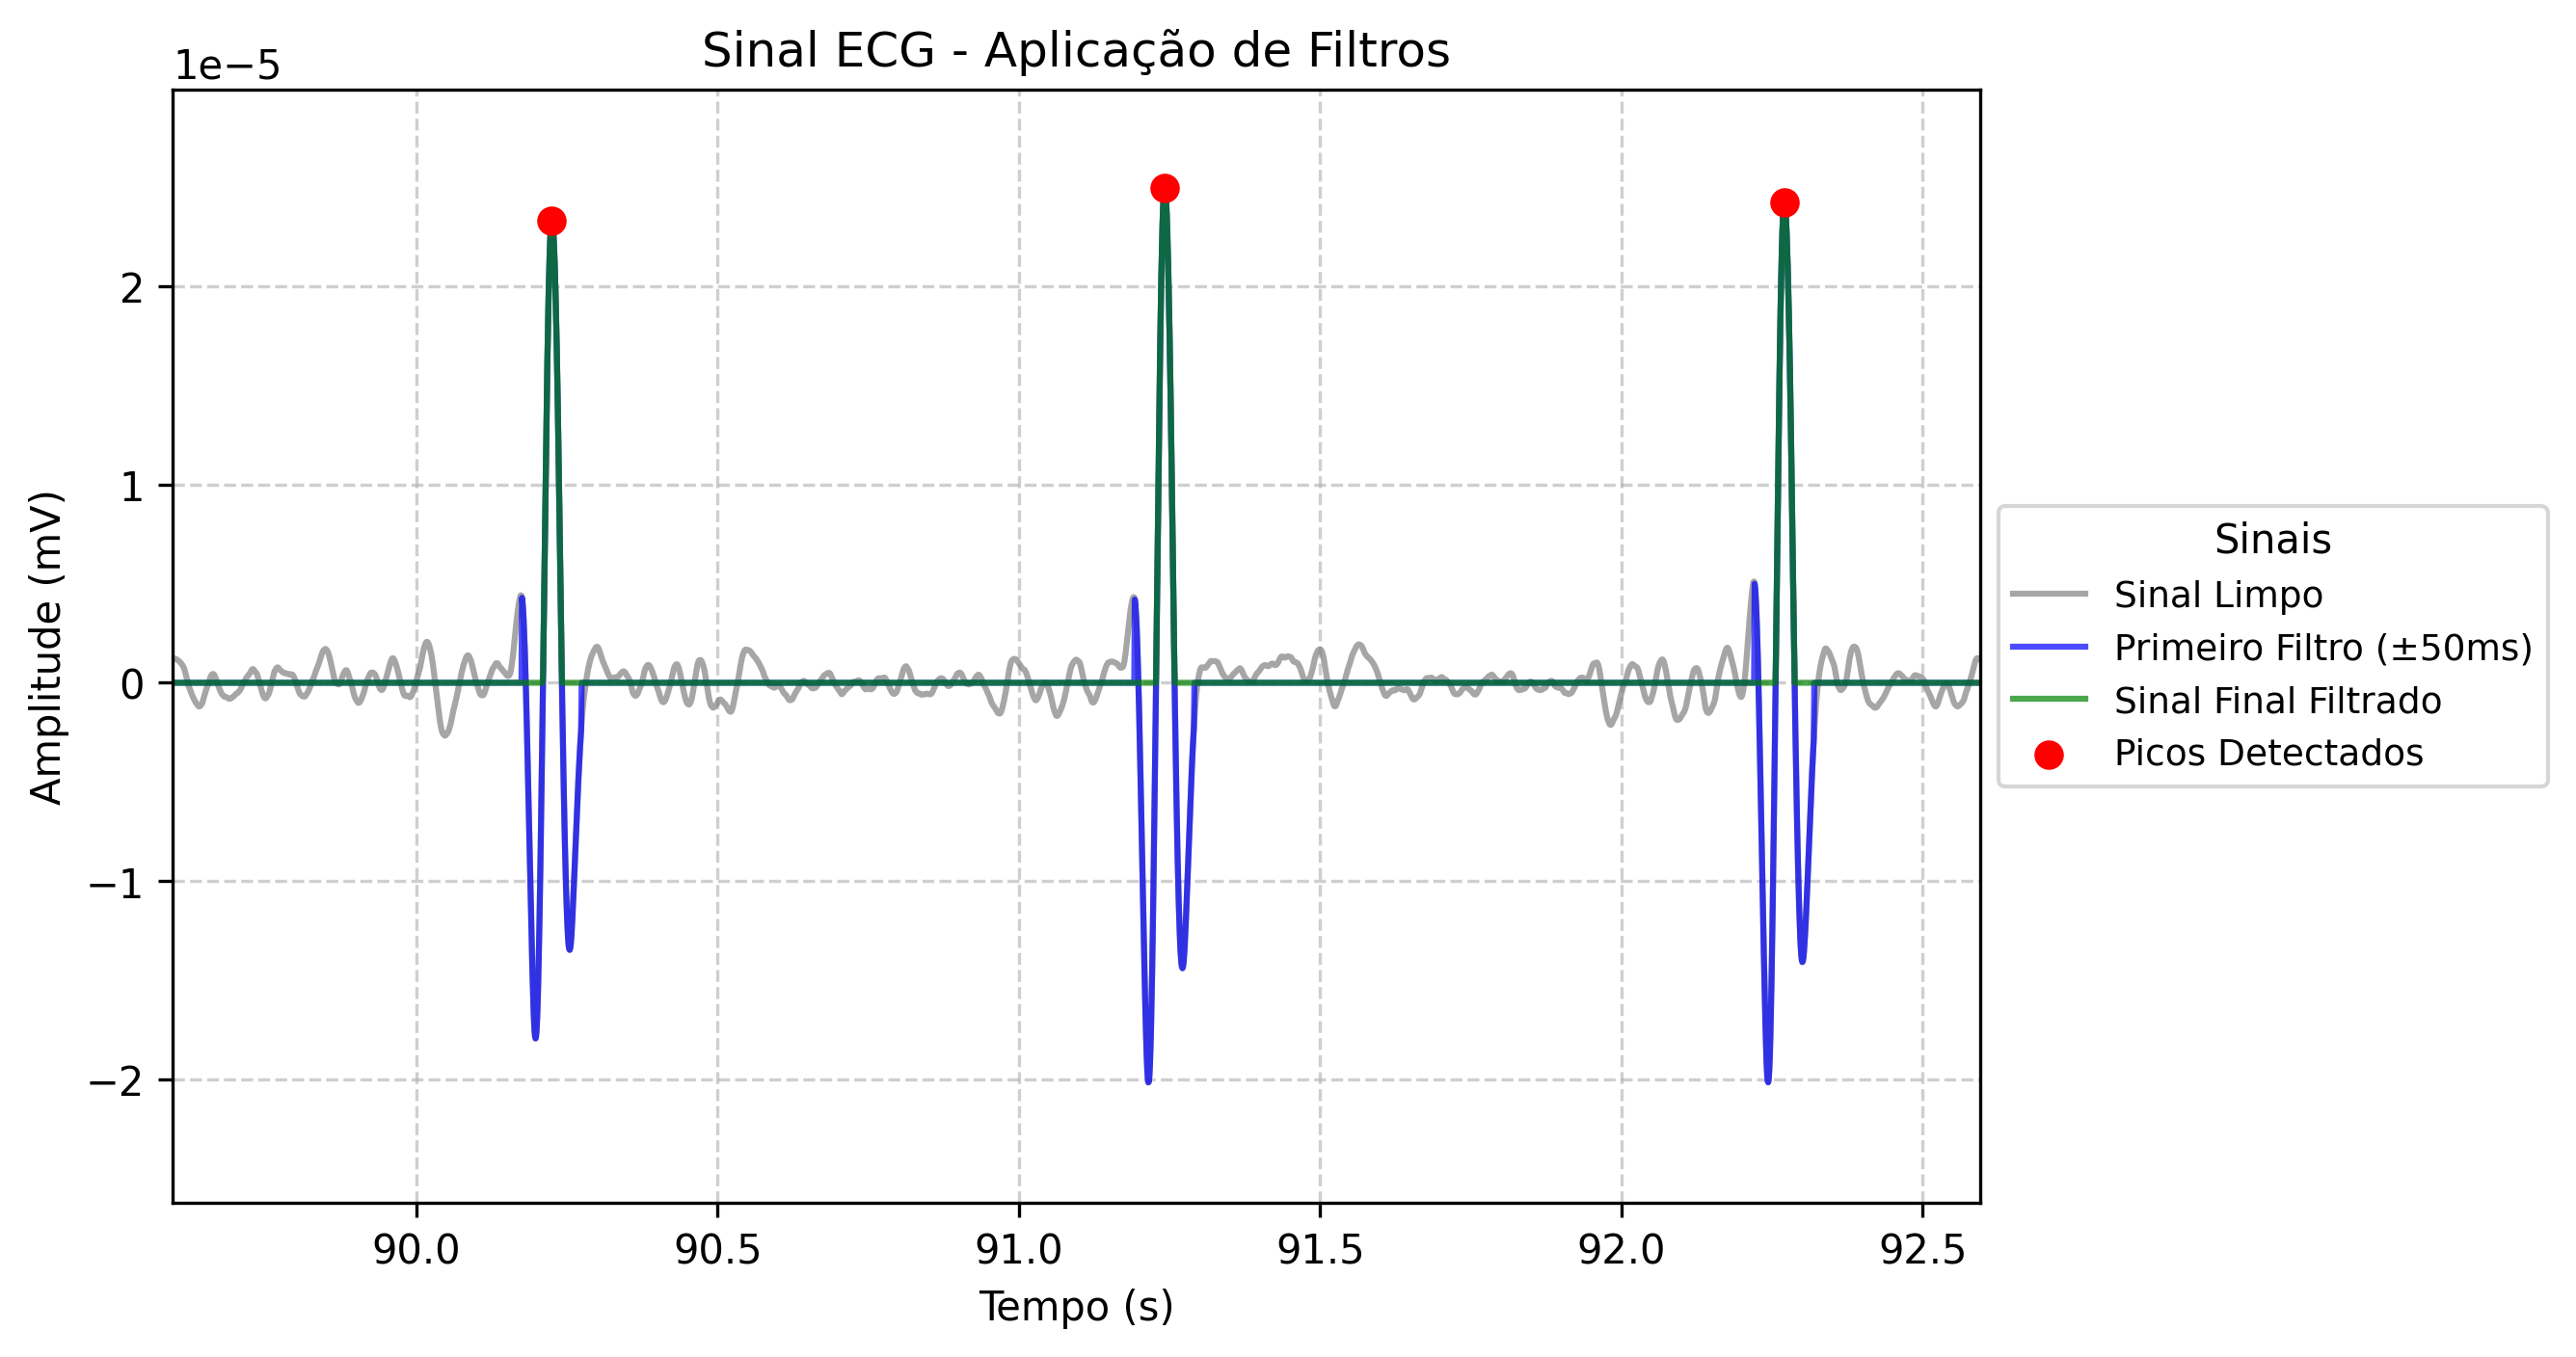
\includegraphics[width=0.8\textwidth]{figs/2_preprocessamento_ecg/2_Sinal_ECG_-_Aplicação_de_Filtros_zoom.png}
    \caption{Exemplo de aplicação de filtros complementares ao sinal de ECG, destacando a morfologia dos picos R (em vermelho).}
    \label{fig:ecg_filtros_aplicados}
\end{figure}

\subsubsection{Geração de Sinais Senoidais e Análise de Fase}

Para aprimorar a análise de sincronização de fase entre os sinais de EEG e ECG, o sinal de ECG foi transformado em uma representação senoidal. Essa transformação foi adotada pelos seguintes motivos:

\begin{itemize}
    \item \textbf{Definição Clara do Ciclo Cardíaco:} Ao utilizar os R-peaks para delimitar cada ciclo, a transformação em uma onda senoidal permite definir de forma inequívoca o início e o fim do ciclo cardíaco, proporcionando um marcador preciso para segmentar os períodos de interesse.
    \item \textbf{Extração Precisa da Fase:} Uma onda senoidal apresenta uma variação linear de fase ao longo do tempo, o que facilita a extração da fase instantânea por meio da Transformada de Hilbert. Essa linearidade contribui para uma determinação mais robusta e consistente da fase, essencial para análises de sincronização.
    \item \textbf{Facilitação da Análise de Sincronização:} Técnicas de sincronização de fase, como o CF-PLM (uma variante do PLV para análise cross-frequency), funcionam melhor quando a fase é clara e bem definida. A representação senoidal torna a fase do ECG mais nítida, permitindo que os algoritmos capturem de forma mais precisa a relação de sincronização entre os ritmos neurais (EEG) e o ritmo cardíaco.
    \item \textbf{Robustez à Variabilidade e Ruído:} O ECG bruto possui características de pico acentuado e variabilidade que podem dificultar a obtenção de uma fase contínua e suave. Ao converter o sinal para uma forma senoidal, essas irregularidades são suavizadas, o que melhora a robustez do método de extração de fase mesmo em presença de ruídos ou artefatos.
    \item \textbf{Integração com a Análise de EEG:} Como os sinais de EEG são frequentemente filtrados para se aproximarem de formas quase senoidais, padronizar a representação do ECG para uma forma senoidal facilita a integração dos dois tipos de sinais na análise de sincronização, permitindo comparações diretas e métodos de análise cross-frequency mais eficazes.
\end{itemize}

A Figura~\ref{fig:ecg_comparacao_fase} ilustra a comparação de fase entre o sinal de ECG filtrado, o sinal senoidal gerado e um sinal simulado, evidenciando a coerência de fase entre eles.

\begin{figure}[htb]
    \centering
    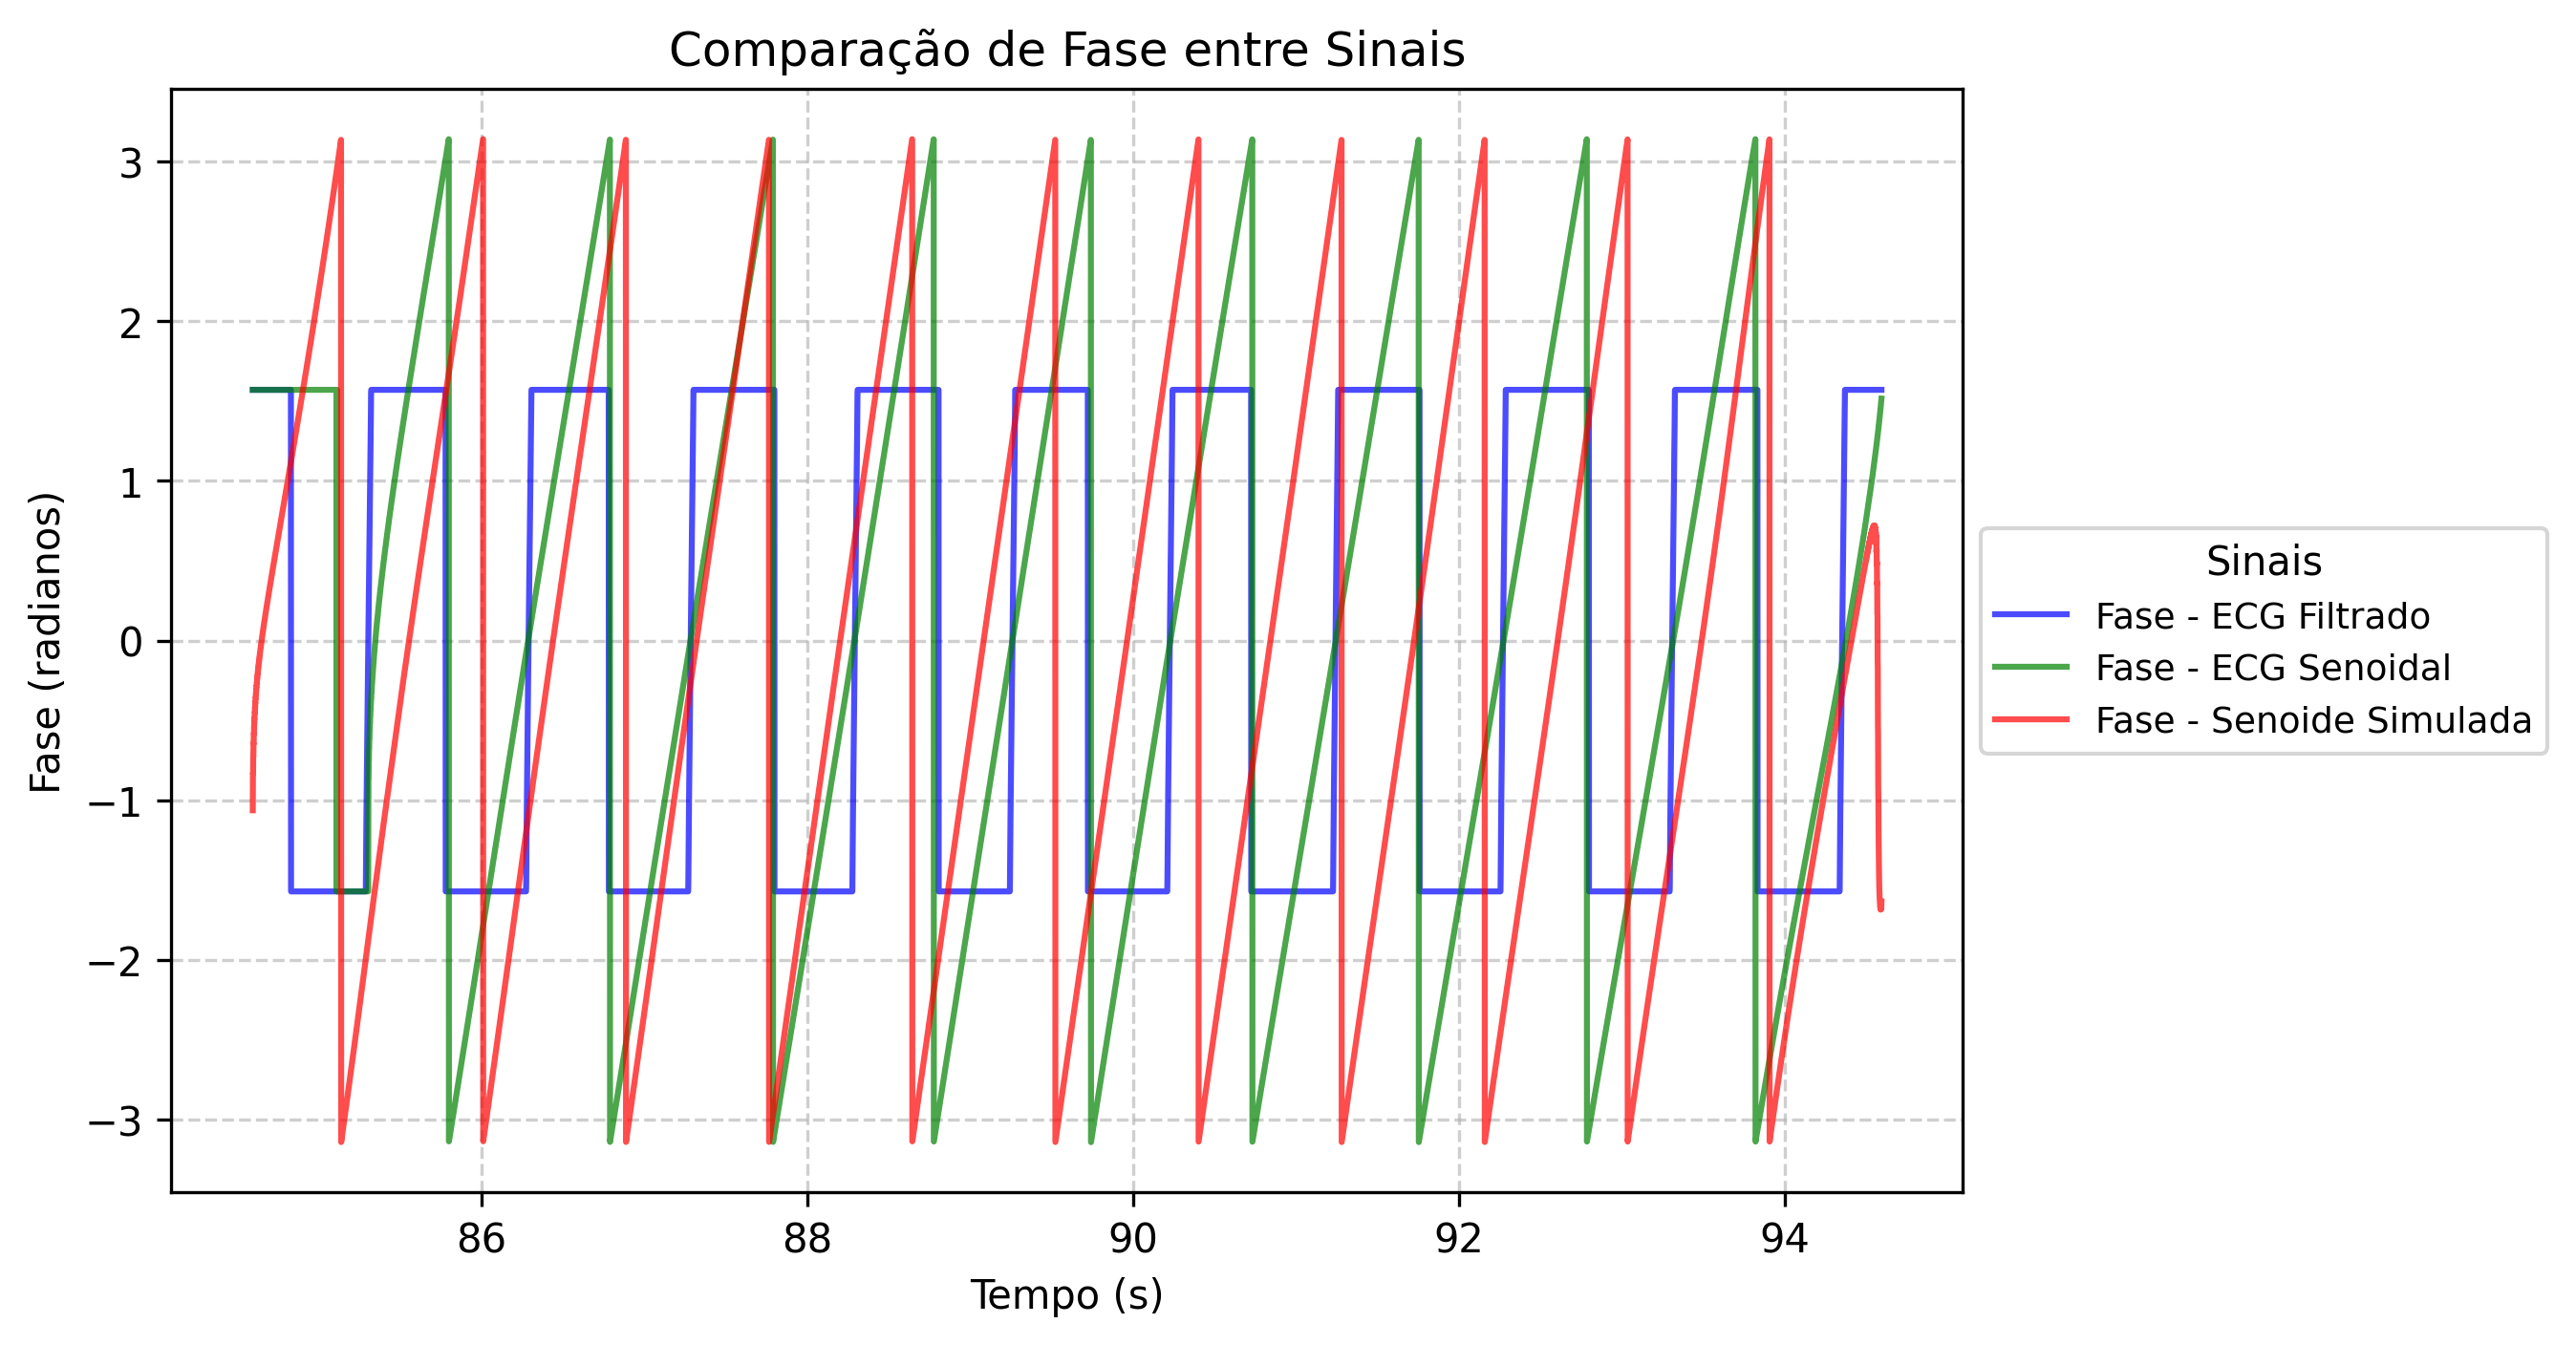
\includegraphics[width=0.8\textwidth]{figs/2_preprocessamento_ecg/3_Comparação_de_Fase_entre_Sinais.png}
    \caption{Exemplo de comparação de fase entre o ECG filtrado (azul), o ECG senoidal (verde) e um sinal simulado (vermelho). A boa concordância entre as fases indica que o procedimento de geração do sinal senoidal e a extração de fase são consistentes.}
    \label{fig:ecg_comparacao_fase}
\end{figure}

Em suma, a transformação do ECG em um sinal senoidal não apenas define de forma clara o ciclo cardíaco, mas também possibilita a extração de uma fase contínua, fundamental para a análise de sincronização de fase entre EEG e ECG utilizando métodos que envolvam extração de fase, tais quais os utilizados neste estudo.

\subsubsection{Estrutura do Dado Final e Armazenamento}

O DataFrame final resultante do processamento do ECG integra:
\begin{itemize}
    \item \textbf{Tempo:} Timestamps sincronizados.
    \item \textbf{Sinal Bruto (EMG):} Valor original do sinal.
    \item \textbf{Sinal Limpo (ECG):} Versão filtrada do sinal.
    \item \textbf{Picos:} Indicador binário dos R-peaks detectados.
    \item \textbf{First Filtered:} Sinal obtido após a aplicação do filtro de janela (±50 ms).
    \item \textbf{Final Filtered:} Sinal final obtido após a combinação dos filtros.
    \item \textbf{ECG Senoidal:} Sinal senoidal derivado dos R-peaks.
\end{itemize}
Este conjunto de dados foi exportado em formato CSV.

\part{Análises e Resultados}
\chapter{Métodos de Análise de Sincronização de Fase}
\label{chap:6_metodos_de_analise_de_sincronizacao_de_fase}

Neste capítulo, apresentamos os fundamentos teóricos e práticos dos métodos empregados para analisar a sincronização de fase entre sinais fisiológicos. Para este estudo, optamos por utilizar o Phase Lag Index (PLI) para quantificar a sincronização entre canais de EEG (mesma frequência) e o Cross-Frequency Phase Linearity Measurement (CF-PLM) para avaliar o acoplamento cross-frequency entre EEG e ECG. Adicionalmente, o tradicional Phase Locking Value (PLV) foi testado para comparação, cujos resultados encontram-se disponíveis no anexo.

\section{Fundamentos dos Métodos}

A análise de sincronização de fase visa quantificar a consistência da diferença de fase entre dois sinais ao longo do tempo. Diversas abordagens foram desenvolvidas, que podem ser classificadas em técnicas baseadas em modelos e métodos \textit{data-driven}, conforme discutido em \cite{seraj2018cerebral}. O conceito de sincronização de fase --- definido como o ajuste temporal dos ritmos de dois sinais, mesmo que suas amplitudes não estejam correlacionadas --- é essencial para a compreensão dos processos neurais \cite{seraj2018cerebral}.

Para extrair a fase dos sinais, técnicas como a Transformada de Hilbert são amplamente empregadas. Entretanto, alternativas como a Transformada de Fourier e os wavelets (por exemplo, o wavelet de Morlet) oferecem uma decomposição tempo-frequencial dos sinais. Embora a Transformada de Fourier seja eficaz para sinais estacionários, sua interpretação se torna mais complexa quando o conteúdo em frequência varia com o tempo\textsuperscript{\cite{singh2024evaluating}}. Adicionalmente, embora este estudo se concentre no acoplamento fase-fase, vale mencionar que abordagens para acoplamento fase-amplitude também foram comparadas. Hülsemann et al. (2019) \cite{hulsemann2019quantification} demonstraram que o Mean Vector Length (MVL) é particularmente sensível às modulações na força e largura do acoplamento, enquanto o Modulation Index (MI) apresenta maior robustez em condições de dados curtos e ruidosos, sugerindo que ambos os índices podem complementar a análise.

Outro aspecto fundamental é o mecanismo de feedback denominado \emph{reentry}, que exige relações temporais específicas para que os neurônios sincronizem suas taxas de disparo\textsuperscript{\cite{seraj2018cerebral}}. Essa dinâmica reforça a relevância da sincronização de fase na medição da conectividade cerebral. Além disso, a fase dos sinais é considerada “pura” e menos suscetível a artefatos em comparação com a amplitude, que pode ser fortemente influenciada por impedâncias ou movimentos (por exemplo, de olhos e músculos faciais)\textsuperscript{\cite{seraj2018cerebral}}. Essa característica torna a informação de fase uma ferramenta valiosa para investigar a comunicação entre áreas cerebrais.

Embora abordagens baseadas em modelos estatísticos, como as propostas por Nadalin et al. \cite{nadalin2019statistical}, sejam úteis para avaliar acoplamentos fase-amplitude e amplitude-amplitude, elas podem não capturar completamente as relações dinâmicas entre as fases dos sinais. A dependência de pressuposições estatísticas e o rigor no controle de covariáveis podem limitar a identificação de padrões de sincronização mais complexos, especialmente em dados de estado de repouso, onde os acoplamentos fase-fase entre diferentes bandas de EEG e ECG tendem a ser mais variáveis e não lineares.

A conectividade funcional pode ser explorada sob a ótica da interação contínua entre diferentes regiões cerebrais. Conforme descrito em\textsuperscript{\cite{sorrentino2022detection}}, diversas áreas precisam transferir informações constantemente para suportar respostas comportamentais complexas. Ademais, como ressaltado em\textsuperscript{\cite{sorrentino2022detection}}, existem inúmeras métricas para detectar interações \textit{cross-frequency}, que variam desde acoplamentos fase-amplitude até acoplamentos fase-fase. Essa diversidade de abordagens é fundamental quando se lida com dados de repouso, nos quais diferentes bandas interagem simultaneamente.

Outra vantagem das análises modernas é o uso de gravações multicanais, que possibilitam identificar padrões fisiologicamente interpretáveis de acoplamento entre frequências. Técnicas de redução de dimensionalidade e separação de fontes, conforme mencionado em\textsuperscript{\cite{cohen2017multivariate}}, permitem isolar padrões de atividade que seriam difíceis de detectar em sinais monofacetados. Ademais, o framework de decomposição generalizada (gedCFC), apresentado por Cohen (2017)\textsuperscript{\cite{cohen2017multivariate}}, tem sido utilizado para superar limitações dos métodos tradicionais, especialmente quando se trata de sinais não estacionários.

A discussão sobre acoplamento cross-frequency também envolve a consideração de que a fase pode codificar mais informações do que a amplitude, como evidenciado em estudos recentes \cite{autor2020}. Ren et al. (2022) \cite{ren2022multi} revisaram o uso do acoplamento de fase (phase-phase coupling) na montagem de redes cerebrais, demonstrando que abordagens multi-granulares podem revelar padrões robustos de sincronização cross-frequency. Diversos estudos têm mostrado que a interação entre diferentes bandas de frequência — conhecida como cross-frequency coupling (CFC) — ocorre em regiões como o hipocampo, o córtex pré-frontal e o sensorial, tanto em humanos quanto em primatas não-humanos \cite{mormann2005phase, canolty2006high, jensen2007cross, khamechian2020decoding}. Pesquisas de Dimitriadis et al. \cite{dimitriadis2015cognitive} e Davoudi et al. \cite{davoudi2021prefrontal} exploraram o acoplamento entre bandas theta e alpha, bem como mecanismos de acoplamento alpha-gamma durante tarefas cognitivas. No contexto de pacientes com AVC, estudos focados na análise do CFC durante movimentos ou tarefas executivas evidenciam a necessidade de investigar processos de imaginação motora para capturar interações mais amplas entre regiões cerebrais.

Entretanto, extrair características efetivas do CFC é mais desafiador do que analisar o acoplamento intrafrequencial, pois os dados são mais complexos e contêm informações ocultas que requerem análises profundas para elucidar os mecanismos fisiológicos subjacentes \cite{ren2022multi}. Essa dificuldade ressalta a importância do desenvolvimento de métodos robustos, como o CF-PLM, para explorar os padrões de sincronização cross-frequency.

\subsection{Phase Lag Index (PLI)}

O PLI é um índice amplamente utilizado para medir a sincronização de fase entre sinais que operam na mesma faixa de frequência, como os canais de EEG dentro de uma mesma banda. Ao contrário do Phase Locking Value (PLV), o PLI é robusto à mistura de sinais e aos efeitos de condução de volume, pois foca na assimetria da distribuição das diferenças de fase. Especificamente, ele desconsidera valores próximos de zero — que podem resultar de sincronizações espúrias frequentemente induzidas por fontes comuns ou artefatos — concentrando-se apenas em atrasos de fase que são mais informativos sobre a interação funcional.

Conforme discutido por \citeauthor{seraj2018cerebral} (\citeyear{seraj2018cerebral}), o PLI apresenta vantagens metodológicas ao fornecer uma medida mais pura da sincronização de fase, eliminando a influência de picos decorrentes do volume conduction. O cálculo do PLI envolve a estimativa do sinal espectral cruzado entre dois sinais, onde, em vez de realizar a média dos vetores complexos, utiliza-se a média da parte imaginária desses vetores (por meio da função \texttt{sign}). Dessa forma, o PLI varia entre 0 e 1, com 0 indicando ausência de acoplamento efetivo (possivelmente devido a efeitos de volume conduction) e 1 indicando um acoplamento de fase robusto e consistentemente direcionado.

Além disso, variantes do PLI, como o weighted Phase Lag Index (wPLI), foram desenvolvidas para aumentar a robustez contra efeitos espúrios e ruídos. No wPLI, apenas os componentes imaginários da diferença de fase são considerados e ponderados, enfatizando atrasos reais na comunicação neural. Qiu e Luo (2024) \cite{qiu2024brain} demonstraram que o wPLI é particularmente eficaz para a análise da conectividade funcional, uma vez que a extração da fase instantânea — realizada via transformada de Hilbert ou Fourier —, seguida do cálculo da diferença de fase e da aplicação de uma média ponderada dos componentes imaginários, resulta em uma métrica mais precisa na captação dos atrasos na transmissão neural.

Em resumo, enquanto o PLI tradicional fornece uma estimativa robusta da sincronização de fase ao desconsiderar sincronizações imediatas (próximas a zero), o wPLI refina essa abordagem atribuindo pesos aos atrasos de fase, minimizando a influência de artefatos e do volume de condução. Essas características tornam ambas as medidas especialmente úteis na investigação da conectividade funcional em EEG, permitindo a identificação de interações neurais genuínas mesmo em cenários de sinais dinâmicos e não estacionários.

\subsection{Cross-Frequency Phase Linearity Measurement (CF-PLM)}

O CF-PLM é um método desenvolvido para analisar a sincronização de fase entre sinais que operam em frequências distintas, ou seja, para detectar o acoplamento cross-frequency. Essa abordagem é especialmente útil para avaliar a relação entre os ritmos neurais do EEG (tipicamente de alta frequência) e o ritmo cardíaco do ECG (geralmente de baixa frequência).

De acordo com \citeauthor{sorrentino2022detection} (\citeyear{sorrentino2022detection}), o método estende o conceito de Phase Linearity Measurement (PLM) para a análise de sincronização n:m, dispensando hipóteses a priori sobre as frequências envolvidas. Além disso, abordagens baseadas em decomposição, como o framework gedCFC proposto por Cohen (2017) \cite{cohen2017multivariate}, demonstram robustez na identificação de padrões de acoplamento fase-fase mesmo em dados multicanais não estacionários.

O procedimento do CF-PLM compreende os seguintes passos:

\begin{enumerate}
    \item \textbf{Cálculo dos Sinais Analíticos:} Para os sinais de interesse, \(x(t)\) e \(y(t)\), obtém-se suas representações analíticas, \(x_{\mathrm{an}}(t)\) e \(y_{\mathrm{an}}(t)\), por meio da Transformada de Hilbert. Essas representações fornecem, respectivamente, as fases \(\phi_x(t)\) e \(\phi_y(t)\).
    \item \textbf{Construção do Sinal Interferométrico:} Calcula-se o sinal interferométrico \(z(t)\) utilizando a fórmula:
    \[
    z(t) = \frac{x_{\mathrm{an}}(t)\, y_{\mathrm{an}}^*(t)}{\lvert x_{\mathrm{an}}(t)\rvert\, \lvert y_{\mathrm{an}}(t)\rvert} = e^{i\Delta \phi(t)},
    \]
    onde \(\Delta \phi(t) = \phi_x(t) - \phi_y(t)\) representa a diferença de fase instantânea entre os sinais. Como \(z(t)\) possui amplitude unitária, ele isola a informação de fase.
    \item \textbf{Análise da Densidade Espectral de Potência (PSD):} Por meio da Transformada de Fourier -- cuja aplicação também é discutida em \cite{seraj2018cerebral} -- calcula-se a PSD de \( z(t) \). Em condições de acoplamento iso-frequencial, o pico da PSD se encontra centralizado em \(f = 0\); já em condições de acoplamento cross-frequency, um pico deslocado indica a diferença entre as frequências dominantes dos sinais. Estudos como o de \cite{chen2023multiple} demonstraram, utilizando PAC, que alterações no acoplamento entre frequências podem ser potenciais biomarcadores. Adicionalmente, Zhang et al. (2023) \cite{zhang2023differences} compararam os padrões de espectro de potência e acoplamento cross-frequency entre pacientes jovens e idosos sob anestesia com sevoflorano, destacando variações na modulação das amplitudes alpha nas fases delta. Embora esse estudo se concentre em PAC, seus achados reforçam a importância das técnicas de análise cross-frequency para compreender as alterações neurofisiológicas em diferentes condições clínicas.
    \item \textbf{Cálculo do CF-PLM:} O índice CF-PLM é obtido integrando a PSD em uma janela estreita, \([f_\Delta - B, f_\Delta + B]\), centrada no pico (onde \(f_\Delta\) representa a diferença de frequência entre os sinais), e normalizando pelo poder total da PSD:
    \[
    \text{CF-PLM} = \frac{\displaystyle\int_{f_\Delta - B}^{f_\Delta + B} SZ(f) \, df}{\displaystyle\int_{-\infty}^{+\infty} SZ(f) \, df}.
    \]
\end{enumerate}

Observa-se que, ao empregar o CF-PLM, dispensa-se a necessidade de hipóteses prévias sobre as relações harmônicas entre os sinais, o que representa uma vantagem significativa quando se trabalha com acoplamento entre sinais cujas frequências podem variar livremente – como é o caso do ECG e do EEG. Adicionalmente, conforme destacado em\textsuperscript{\cite{sorrentino2022detection}}, esse método permite uma exploração abrangente dos dados, identificando quais componentes de frequência estão envolvidos na sincronização.

\subsection{Comparação com o Phase Locking Value (PLV)}

Para fins de validação e comparação, também testamos o PLV, um método tradicional amplamente utilizado para a análise de sincronização de fase. Conforme descrito em \cite{seraj2018cerebral}, o PLV mede a consistência da diferença de fase entre dois sinais na mesma faixa de frequência; entretanto, ele é sensível a ruídos e aos efeitos de volume conduction, o que pode levar à detecção de sincronizações espúrias. Por exemplo, estudos como o de \cite{abubaker2021working} investigaram o acoplamento cruzado entre frequências em tarefas de memória de trabalho utilizando o PLV, sugerindo que padrões específicos de sincronização podem estar associados ao desempenho cognitivo. Contudo, a ausência de técnicas avançadas para mitigar artefatos pode limitar sua aplicabilidade em contextos clínicos.

Adicionalmente, Zhang et al. (2014) \cite{zhang2014phase} investigaram a sincronização de fase durante tarefas cognitivas prolongadas e constataram que, na faixa beta (13--30 Hz), os valores médios de PLV diminuem significativamente tanto em pares inter-hemisféricos (especialmente nas regiões central e parietal) quanto em pares intra-hemisféricos (como entre os eletrodos frontal-parietal, central-parietal e frontal-central). Esses achados ilustram como a sensibilidade do PLV pode ser afetada por estados de fadiga mental, ressaltando suas limitações diante de variações no processamento cognitivo.

Métodos adaptativos, como os propostos por Van Zaen et al. \cite{vanzaen2013adaptive}, também foram investigados para melhorar a detecção de acoplamentos cruzados em sinais não estacionários. Contudo, para o cenário de resting-state EEG-ECG adotado neste estudo, optou-se por utilizar métodos tradicionais, os quais se mostraram mais eficientes na identificação de padrões globais sem a necessidade de rastrear variações temporais finas.

Dessa forma, optamos por utilizar o PLI e o CF-PLM como índices principais para a análise de sincronização, reservando o PLV para comparação e validação, conforme os resultados apresentados no anexo.

É importante ainda considerar que, embora a Transformada de Hilbert seja frequentemente utilizada para extrair a fase instantânea, outros métodos como a Transformada de Fourier e os wavelets oferecem alternativas – cada um com suas vantagens e limitações \cite{seraj2018cerebral}. Por exemplo, a Transformada de Fourier é mais adequada para sinais estacionários, enquanto os wavelets, como o de Morlet, permitem uma análise tempo-frequencial, embora com compromissos em precisão.

Além disso, conforme relatado em \cite{sorrentino2022detection}, as áreas cerebrais precisam transferir informações constantemente para suportar respostas comportamentais complexas, e diversas métricas foram propostas para quantificar essa comunicação. Entre elas, a análise de acoplamento cross-frequency é essencial para entender como diferentes ritmos interagem. Vários estudos \cite{hulsemann2019quantification} destacam que métodos como acoplamento fase-amplitude, bicoerência e fase-locking apresentam vantagens e desafios específicos, o que exige uma escolha cuidadosa do método baseado no tipo de dados e na hipótese experimental. Por fim, abordagens que utilizam registros multicanais, como a decomposição por autovalores generalizada (gedCFC) \cite{cohen2017where}, ampliam as possibilidades de identificação de padrões de conectividade, reforçando evidências de que a fase pode codificar mais informações do que a amplitude.

\subsection{Resumo dos Principais Pontos}

Em síntese, a escolha dos métodos apresentados neste capítulo considerou os seguintes aspectos:

\begin{itemize}
  \item A necessidade de capturar a sincronização de fase de forma robusta, minimizando os efeitos do volume conduction e de ruídos, conforme evidenciado na comparação entre PLI e PLV \cite{seraj2018cerebral, zhang2014phase}.
  \item A importância de abordar acoplamentos cross-frequency sem pressupor relações harmônicas fixas, justificando o emprego do CF-PLM \cite{sorrentino2022detection, seraj2018cerebral, cohen2017multivariate}.
  \item As limitações inerentes a cada técnica de extração de fase – seja via Transformada de Hilbert, Fourier ou wavelets – e a necessidade de selecionar o método mais adequado conforme as características dos sinais \cite{seraj2018cerebral}.
  \item A vantagem de utilizar registros multicanais e técnicas de decomposição avançadas para explorar padrões complexos de conectividade, integrando diferentes escalas temporais e frequenciais \cite{cohen2017multivariate}.
\end{itemize}

Portanto, a combinação dos métodos PLI e CF-PLM, complementada pela comparação com o PLV, fornece uma base sólida para a investigação da sincronização de fase em contextos de alta complexidade, como a interação entre sinais de EEG e ECG.

\section{Validação Experimental com Injeção de Sinais}

Para validar os métodos utilizados neste estudo, foram realizados experimentos com injeção controlada de sinais senoidais sobre dados reais de ECG e EEG, coletados durante sessões experimentais. O objetivo desta validação foi verificar a capacidade dos índices CF-PLM, PLV e PLI em identificar corretamente diferentes níveis e tipos de sincronização de fase artificialmente introduzidos.

A técnica empregada consistiu nas seguintes etapas:
\begin{enumerate}
    \item Seleção de segmentos representativos dos sinais originais de ECG e EEG.
    \item Geração de sinais senoidais com frequências e fases específicas utilizando o modelo de Kuramoto, permitindo o controle preciso das condições experimentais.
    \item Aplicação controlada dos sinais senoidais sobre os sinais originais por meio de máscaras de injeção, variando a porcentagem de contribuição (0\%, 25\%, 50\%, 75\% e 100\%) dos sinais injetados.
    \item Cálculo dos índices CF-PLM, PLV e PLI sobre os sinais modificados para avaliar o desempenho dos métodos de sincronização em diferentes cenários.
\end{enumerate}

Foram conduzidos três cenários principais:

\begin{itemize}
    \item \textbf{Cross-frequency (1~Hz no ECG, 40~Hz no EEG):} Destinado a testar especialmente o índice CF-PLM em situações onde o acoplamento ocorre entre frequências distintas.
    \item \textbf{Same-frequency (10~Hz no ECG e EEG com defasagem):} Avalia a sensibilidade e desempenho de todos os índices quando os sinais possuem a mesma frequência, mas apresentam uma defasagem de fase fixa configurada (\(\pi/4\)).
    \item \textbf{Same-frequency com phase lag zero (ambos 10~Hz sem defasagem):} Cenário idealizado para demonstrar a robustez do PLI contra sincronizações triviais decorrentes de volume conduction.
\end{itemize}

Exemplos dos sinais antes e após a injeção no cenário Cross-frequency são mostrados nas Figuras~\ref{fig:ecg_injection} e~\ref{fig:eeg_injection}, que ilustram a adição de sinais artificiais com frequências distintas sobre o sinal original.


\standardfigure{figs/3_2_testing_connectivity_metrics/1_ECG_Original_vs_Injecao_Cross-frequency.png}
{ECG: comparação entre o sinal original e o sinal senoidal injetado (1~Hz), cenário Cross-frequency.}
{ecg_injection}

\standardfigure{figs/3_2_testing_connectivity_metrics/3_EEG_Original_vs_Injecao_Cross-frequency.png}
{EEG: comparação entre o sinal original e o sinal senoidal injetado (40~Hz), cenário Cross-frequency.}
{eeg_injection}


No cenário Same-frequency, onde tanto o ECG quanto o EEG recebem sinais senoidais com a mesma frequência (10~Hz) mas com uma defasagem de \(\pi/4\), os resultados são ilustrados nas Figuras~\ref{fig:eeg_original_vs_injection_samefreq} e~\ref{fig:eeg_injected_samefreq}. Esses gráficos evidenciam a interferência gerada pela injeção controlada.

\standardfigure{figs/3_2_testing_connectivity_metrics/10_EEG_Original_vs_Injecao_Same-frequency.png}
{EEG original (azul) e sinal de injeção de 10 Hz (vermelho) com pequena defasagem (\(\pi/4\)).}
{eeg_original_vs_injection_samefreq}

\standardfigure{figs/3_2_testing_connectivity_metrics/11_EEG_Injetado_Same-frequency.png}
{Sinal de EEG após a injeção controlada de uma senóide (verde), comparado ao sinal original sem injeção (azul).}
{eeg_injected_samefreq}


Em seguida, extraímos as fases instantâneas utilizando a Transformada de Hilbert e geramos o sinal interferométrico, conforme exemplificado nas Figuras~\ref{fig:fases_instantaneas_samefreq} e~\ref{fig:sinal_interferometrico_samefreq}.

\standardfigure{figs/3_2_testing_connectivity_metrics/12_Passo1_Fases_Same-frequency.png}
{Fases instantâneas extraídas dos sinais EEG e ECG injetados (ambos a 10 Hz).}
{fases_instantaneas_samefreq}

\standardfigure{figs/3_2_testing_connectivity_metrics/13_Passo2_Interferometrico_Same-frequency.png}
{Sinal interferométrico gerado pela diferença de fase instantânea (cenário Same-frequency).}
{sinal_interferometrico_samefreq}


A seguir, calculamos o índice CF-PLM utilizando a Transformada de Fourier (FFT) sobre o sinal interferométrico. A Figura~\ref{fig:fft_psd_samefreq} exemplifica a análise, mostrando o pico em 0 Hz, que ocorre devido ao offset constante de fase entre os sinais de mesma frequência.

\standardfigure{figs/3_2_testing_connectivity_metrics/14_Passo3_FFT_PSD_Same-frequency.png}
{PSD do sinal interferométrico, indicando o pico em 0 Hz devido ao offset constante de fase entre os sinais de mesma frequência.}
{fft_psd_samefreq}

Por fim, analisamos o cenário especial "Same-frequency com Phase Lag Zero", onde as fases dos sinais estão perfeitamente sincronizadas. As Figuras~\ref{fig:zerolag_phases_final} e~\ref{fig:zerolag_difference_final} demonstram que, nesse caso, a diferença de fase se aproxima de zero, evidenciando a robustez do PLI contra sincronizações triviais.

\standardfigure{figs/3_2_testing_connectivity_metrics/15_ZeroLag_Fases_Same-frequency Com Phase Lag Zero.png}
{Fases desenroladas em cenário sem defasagem (10 Hz), com sobreposição quase exata dos sinais.}
{zerolag_phases_final}

\standardfigure{figs/3_2_testing_connectivity_metrics/16_ZeroLag_Diferenca_Fase_Same-frequency Com Phase Lag Zero.png}
{Diferença de fase próxima a zero, indicando ausência completa de defasagem no cenário de Phase Lag Zero.}
{zerolag_difference_final}


O comportamento geral dos índices CF-PLM, PLV e PLI nos diferentes cenários e níveis de injeção é resumido na Figura~\ref{fig:comparativo_metricas}.

\standardfigure{figs/3_2_testing_connectivity_metrics/17_Comparativo_Subplots_Experimentos.png}
{Comparação dos índices CF-PLM, PLV e PLI nos três cenários estudados, em função da porcentagem de injeção aplicada.}
{comparativo_metricas}

Esses resultados justificam a escolha do CF-PLM para a análise de sincronização entre EEG e ECG (cross-frequency) e do PLI para sincronização em frequências iguais, evitando a detecção de acoplamentos triviais, como os decorrentes de volume conduction (phase lag zero). O PLV é reportado apenas para referência complementar, dada sua elevada sensibilidade em condições triviais.

\section{Análise de Conectividade ao Longo do Tempo}
\label{sec:connectivity_over_time}

Para investigar a dinâmica da sincronização ao longo da sessão experimental, os sinais foram segmentados em janelas de 10 segundos, considerando a gravação total de 4 minutos e 30 segundos de cada coleta. Em cada janela, foi calculada uma medida de sincronicidade (PLI, PLV ou CF-PLM) para cada par de canais, para cada banda de frequência, para cada condição (cathodic e sham) e para cada atleta. Em seguida, extraiu-se a mediana desses valores, fornecendo uma medida robusta da conectividade ao longo do tempo para cada configuração. Estudos recentes, como o de \citet{didaci2024how}, demonstraram que o tamanho da janela influencia significativamente a performance das métricas de conectividade em sistemas biométricos baseados em EEG, indicando que janelas entre 8 e 12 segundos oferecem um equilíbrio ideal entre precisão e estabilidade dos dados. Essa evidência reforça a estratégia adotada neste estudo.

Essa abordagem permite visualizar a evolução temporal da sincronização e comparar a estabilidade dos diferentes índices. Ressalta-se que, em nossas análises, enfatizamos o \emph{Wilcoxon RBC} e o p-valor corrigido por Bonferroni como principais indicadores de tamanho de efeito e significância estatística, respectivamente, dada sua robustez em contextos não paramétricos e na presença de variabilidade e outliers.

A seguir, apresentamos as séries temporais obtidas para três métricas principais:

\begin{itemize}
    \item \textbf{CF-PLM (EEG-ECG):} A Figura~\ref{fig:cfplm_time_cat} mostra a mediana do CF-PLM ao longo do tempo para a condição cathodic, refletindo a sincronização cross-frequency entre EEG e ECG.
    \item \textbf{PLI (EEG-EEG):} A Figura~\ref{fig:pli_time_cat} apresenta a mediana do PLI ao longo do tempo para a condição cathodic, indicando a sincronização iso-frequencial entre canais cerebrais.
    \item \textbf{PLV (EEG-EEG):} A Figura~\ref{fig:plv_time_cat} exibe a mediana do PLV ao longo do tempo para a condição cathodic, utilizada aqui para comparação, considerando que o PLV é mais sensível a ruídos e aos efeitos de volume conduction.
\end{itemize}

Cada gráfico é construído a partir dos valores calculados em janelas de 10 segundos, onde a mediana de cada janela representa a medida de sincronicidade de forma robusta, minimizando o impacto de variações pontuais e outliers.

\standardfigure{figs/4_connectivity_over_time/Mediana_do_CF-PLM_ao_longo_do_tempo_(EEG_ECG)_Catódica.png}
{Mediana do CF-PLM ao longo do tempo para a condição cathodic (EEG-ECG). Cada ponto representa a mediana da medida de sincronicidade calculada em janelas de 10 segundos, evidenciando a evolução do acoplamento cross-frequency entre EEG e ECG.}
{cfplm_time_cat}

\standardfigure{figs/4_connectivity_over_time/Mediana_do_PLI_ao_longo_do_tempo_(EEG_EEG)_Catódica.png}
{Mediana do PLI ao longo do tempo para a condição cathodic (EEG-EEG). O gráfico mostra como a sincronização iso-frequencial entre canais cerebrais varia ao longo da gravação.}
{pli_time_cat}

\standardfigure{figs/4_connectivity_over_time/Mediana_do_PLV_ao_longo_do_tempo_(EEG_EEG)_Catódica.png}
{Mediana do PLV ao longo do tempo para a condição cathodic (EEG-EEG). Este índice é apresentado para comparação com o PLI, embora seja mais sensível a ruídos e efeitos de volume conduction.}
{plv_time_cat}
 
\chapter{Análise de Distribuição e Normalidade}
\label{chap:analise_distribuicao_normalidade}
Nesta seção, investigamos a forma das distribuições das métricas de conectividade, tanto em seus valores ``puros'' quanto nas diferenças (\texttt{median\_diff}) entre as condições (Pós – Pré). Inicialmente, apresentamos as distribuições originais das métricas específicas \textbf{(PLI para EEG-EEG e CF-PLM para EEG-ECG)} que serão mantidas para análise. Em seguida, explicamos que, para testar o efeito da estimulação, calculamos a diferença entre os valores pós e pré (por exemplo, \emph{pós-sham} menos \emph{pré-sham}), e por fim discutimos a escolha dos testes estatísticos com base nessas distribuições.

\section{Distribuição das Métricas de Conectividade}
Antes de subtrair os valores pré dos pós, as métricas de conectividade foram extraídas diretamente dos sinais, refletindo as medidas originais sem a influência do efeito de estimulação. As distribuições ``puras'' são ilustradas nas Figuras~\ref{fig:pli_eeg_eeg} (EEG-EEG, PLI) e~\ref{fig:cfplm_eeg_ecg} (EEG-ECG, CF-PLM):
\begin{itemize}
    \item \textbf{PLI (EEG-EEG):} Avalia a sincronização de fase iso-frequencial entre sinais de canais de EEG.
    \item \textbf{CF-PLM (EEG-ECG):} Mede o acoplamento \textit{cross-frequency} entre o EEG e o ciclo cardíaco obtido via ECG.
\end{itemize}

As faixas de frequência investigadas incluem: delta, theta, alpha, beta e gamma.


% -----------------------------------------------------------------------------  
% PLI (EEG-EEG)  
% -----------------------------------------------------------------------------  
\standardfigure{figs/3_1_connectivity_metrics/Distribuição_de_PLI_(EEG-EEG)_por_Banda.png}
{Distribuição de PLI (EEG–EEG) por banda. Nota-se uma clara concentração de valores próximos a zero em todas as bandas de frequência, com a maioria situada entre 0 e 0.2. As bandas rápidas (beta e gamma) apresentam curvas mais estreitas e concentradas perto de zero. Já as bandas mais lentas (delta, theta e alpha), embora também centradas próximo a zero, exibem caudas superiores maiores, especialmente a banda delta (a mais lenta) onde se destacam alguns valores próximos a 1 (excepcionalmente altos nesta distribuição).}
{pli_eeg_eeg}


% -----------------------------------------------------------------------------  
% CF-PLM (EEG-ECG)  
% -----------------------------------------------------------------------------  
\standardfigure{figs/3_1_connectivity_metrics/Distribuição_de_CF-PLM_(EEG-ECG)_por_Banda.png}
{Distribuição de CF-PLM (EEG--ECG) por banda. Observa-se que é praticamente inexistente valores muito próximos a zero. A maior parte encontra-se entre 0.05 e 0.20. A depender da banda de frequência analisada, é possível observar um deslocamento de seus dados em relação às demais. No geral, é possível observar que quanto mais rápidas as bandas de frequência (e.g. gamma), menores os valores de CF-PLM, e menos densos (curvas mais pontudas). Quanto mais lentas (e.g. delta), maiores os valores de CF-PLM, e mais densos (curvas menos pontudas).}
{cfplm_eeg_ecg}

No geral, observamos que:
\begin{itemize}
    \item \textbf{EEG--EEG (PLI)}: A distribuição exibe variabilidade entre as bandas. Enquanto a maioria dos valores se concentra próxima de zero (indicando baixa estabilidade de fase), algumas bandas -- sobretudo \emph{alpha} e \emph{gamma} -- apresentam caudas mais extensas, sugerindo pares de canais com maior \emph{phase-locking} (Figura~\ref{fig:pli_eeg_eeg}).
    \item \textbf{EEG--ECG (CF-PLM)}: A maior parte dos valores se acumula em torno de zero, evidenciando um acoplamento \textit{cross-frequency} tipicamente baixo entre o EEG e o ciclo cardíaco. Ainda assim, há um leve deslocamento em faixas mais lentas (especialmente \emph{delta} e \emph{theta}), o que indica a possibilidade de sincronia pontual em alguns pares (Figura~\ref{fig:cfplm_eeg_ecg}).
\end{itemize}

Essas observações fornecem uma visão inicial do comportamento das métricas ``puras'' de conectividade, servindo de base para a comparação entre as condições (Pós e Pré), que será apresentada a seguir.

\section{Distribuição das Diferenças (\texttt{median\_diff})}
Para avaliar o efeito da estimulação \textit{cathodic} versus \textit{sham}, calculamos a diferença entre os valores medidos após a intervenção (Pós) e os valores obtidos antes (Pré). Essa diferença representa a mudança ocorrida na métrica mediana do índice específico, sendo positiva para aumentos e negativa para reduções:

\[
\texttt{median\_diff} = (\text{pós condição x}) - (\text{pré condição x}),
\]
o que visa isolar o efeito da intervenção, removendo variações comuns que estariam presentes independentemente da estimulação.

As distribuições dessas diferenças foram avaliadas por meio de histogramas com \textit{cross-frequency} (KDE) para as métricas utilizadas nesta análise (PLI para EEG--EEG e CF-PLM para EEG--ECG). Os resultados são apresentados nas Figuras~\ref{fig:pli_freq_eeg_eeg} e~\ref{fig:cf_plm_freq_eeg_ecg}.

\standardfigure{figs/6_distribuicao_metricas_conectividade/Distribuição_da_Diferença_da_PLI_(Pós_-_Pré)_por_Faixa_de_Frequência_EEG_EEG.png}
{Distribuição da diferença da PLI (Pós -- Pré) em EEG--EEG, por faixa de frequência.}
{pli_freq_eeg_eeg}

\standardfigure{figs/6_distribuicao_metricas_conectividade/Distribuição_da_Diferença_da_CF-PLM_(Pós_-_Pré)_por_Faixa_de_Frequência_EEG_ECG.png}
{Distribuição da diferença da CF-PLM (Pós -- Pré) em EEG--ECG, por faixa de frequência.}
{cf_plm_freq_eeg_ecg}

Na Figura~\ref{fig:pli_freq_eeg_eeg} (diferença da PLI em EEG--EEG), podemos observar:
\begin{itemize}
    \item \textbf{Alpha e Beta}: distribuições com picos relativamente bem-definidos próximos de zero, porém com caudas que se estendem para valores positivos e negativos. Isso indica que, embora a maioria dos pares de canais não apresente mudanças extremas de \emph{phase-locking}, há casos em que a PLI sofre variações mais intensas (tanto de aumento quanto de redução).
    \item \textbf{Delta e Theta}: apresentam formatos mais “achatados” (\emph{platocúrticos}), com uma região larga de valores ao redor de zero em vez de um pico pontudo. Sugere-se, assim, que múltiplos pares sofrem pequenas variações dispersas, em vez de convergirem para um valor dominante.
    \item \textbf{Gamma}: exibe uma curva um pouco mais pontuda, ainda que com assimetria leve. Isso pode significar que, em alguns pares, a diferença entre pós e pré se concentra de forma mais coesa em torno de um desvio particular (positivo ou negativo), enquanto a maioria dos pares permanece próxima de zero.
\end{itemize}

Já na Figura~\ref{fig:cf_plm_freq_eeg_ecg} (diferença da CF-PLM em EEG--ECG), o comportamento difere:
\begin{itemize}
    \item \textbf{Gamma}: é a única banda que se aproxima de uma forma mais simétrica e quase gaussiana em torno de zero, indicando que os valores de diferença se distribuem de modo relativamente uniforme, com menor propensão a distorções ou caudas prolongadas.
    \item \textbf{Delta, Alpha e Theta}: exibem curvas mais “achatadas”, sugerindo novamente distribuições \emph{platocúrticas}. O pico central menos pronunciado e a largura mais acentuada indicam variações difusas em torno de zero (seja aumento ou redução), sem um valor predominante.
    \item \textbf{Beta}: apresenta uma assimetria mais clara (cauda se estendendo em uma das direções), apontando que uma fração dos pares EEG--ECG tende a exibir diferenças (Pós $-$ Pré) mais extremas, enquanto a maioria se mantém próxima de zero.
\end{itemize}

Esses perfis de dispersão são fundamentais para a escolha dos testes estatísticos, que será abordada no próximo capítulo, além de fornecerem pistas sobre como as diferentes faixas de frequência podem responder à neuromodulação em termos de sincronização de fase.

\subsubsection{Exemplo Individual por Métrica e Banda}
Para ilustrar de forma mais específica o comportamento das distribuições em um caso individual, a Figura~\ref{fig:median_cf_plm_diff_ath4_alpha_eeg_ecg} exibe a diferença da métrica \texttt{median\_cf\_plm\_diff} (Pós -- Pré) para o atleta 4, na banda \emph{alpha}, considerando todos os pares EEG--ECG. Já a Figura~\ref{fig:median_pli_diff_ath4_alpha_eeg_eeg} apresenta a diferença da \texttt{median\_pli\_diff} para o mesmo atleta e banda, mas agora em pares EEG--EEG.

\standardfigure{figs/5_connectivity_metrics_individual_distribution/median_cf_plm_diff_athlete_4_alpha_EEG_ECG.png}
{Distribuição da \texttt{median\_cf\_plm\_diff} (Pós -- Pré) para o atleta 4, banda \emph{alpha}, em pares EEG--ECG.}
{median_cf_plm_diff_ath4_alpha_eeg_ecg}

\standardfigure{figs/5_connectivity_metrics_individual_distribution/median_pli_diff_athlete_4_alpha_EEG_EEG.png}
{Distribuição da \texttt{median\_pli\_diff} (Pós -- Pré) para o atleta 4, banda \emph{alpha}, em pares EEG--EEG.}
{median_pli_diff_ath4_alpha_eeg_eeg}

Nesses gráficos, cada curva KDE (azul para \textit{cathodic}, vermelha para \textit{sham}) reflete como os valores de diferença (Pós $-$ Pré) se distribuem entre todos os pares de canais daquele atleta e banda de frequência. Um deslocamento maior de uma curva em relação à outra indica uma tendência geral de aumento (deslocamento à direita) ou redução (deslocamento à esquerda) na métrica pós-estimulação, enquanto uma sobreposição acentuada sugere pouca variação entre as condições. 

No exemplo da Figura~\ref{fig:median_cf_plm_diff_ath4_alpha_eeg_ecg}, observa-se que a curva azul (\textit{cathodic}) está levemente à direita da curva vermelha (\textit{sham}), indicando um ligeiro aumento na \texttt{median\_cf\_plm\_diff} para a maioria dos pares. Já na Figura~\ref{fig:median_pli_diff_ath4_alpha_eeg_eeg}, as curvas mostram maior sobreposição, sugerindo que a diferença na \texttt{median\_pli\_diff} entre \textit{cathodic} e \textit{sham} é menos pronunciada.

Embora não seja o foco principal deste estudo, a análise individual por atleta e banda oferece uma visão clara sobre a variabilidade intra e intersujeitos, além de evidenciar como a neuromodulação pode afetar a conectividade de modo heterogêneo. Posteriormente, analisamos cada par de canal em cada faixa de frequência, aprofundando a avaliação dos efeitos significativos da intervenção.

\section{Verificação de Normalidade e Escolha do Teste Estatístico}
Para determinar o tipo de teste estatístico mais adequado (paramétrico ou não-paramétrico), realizamos a verificação da normalidade das distribuições de interesse. Aplicamos os testes de Shapiro-Wilk e Kolmogorov-Smirnov para cada combinação de grupo de canais (EEG--EEG ou EEG--ECG) e faixa de frequência, tanto para as métricas de PLI quanto para as de CF-PLM. 
Além disso, considerando o grande número de observações em cada grupo, mesmo desvios leves podem resultar em p-valores extremamente baixos, justificando o uso de vários testes de normalidade para reforçar a robustez da análise.}

\paragraph{Considerações:}
\begin{itemize}
    \item \textbf{Tamanho amostral:} Como dispomos de grande quantidade de observações após a agregação dos dados, mesmo desvios sutis em relação à normalidade podem levar à rejeição da hipótese nula nos testes de normalidade. 
    Adicionalmente, aplicamos diversos testes (Anderson-Darling, D'Agostino, Jarque-Bera, Lilliefors) para abranger diferentes perspectivas de assimetria e curtose.}
    \item \textbf{Forma das distribuições:} Embora muitos histogramas apresentem uma simetria visual aparente, a análise considerando todos os atletas e condições agrupados revela que cada banda de frequência exibe um padrão próprio de distribuição. Isso sugere que, apesar da simetria, existem características distintas em cada banda, reforçando a importância de análises separadas por faixa de frequência para compreender melhor os efeitos da estimulação nas métricas de conectividade.
    \item \textbf{Interpretação:} Quando os valores de p na maioria das distribuições são inferiores a 0.05, adotamos testes não-paramétricos (como \textit{Wilcoxon signed-rank} ou \textit{Mann-Whitney}) para as análises de inferência.
\end{itemize}

Além desses testes de normalidade, avaliamos também as medidas de assimetria (\emph{skewness}) e curtose (\emph{kurtosis}) para confirmar a adequação de testes paramétricos ou reforçar o uso de métodos não-paramétricos. 
Observou-se que a remoção de \textit{outliers} via Intervalo Interquartil (IQR) ou \textit{Empirical Cumulative Distribution-based Outlier Detection} (ECOD) reduziu a amplitude de variação em alguns casos, mas não eliminou a não-normalidade das distribuições, mantendo inviável o uso de testes paramétricos.

Com base nesses resultados, prosseguimos para as etapas de análise estatística.

\section{Testes de Normalidade e Decisão sobre o Tipo de Teste Estatístico}
Dando seguimento aos procedimentos descritos, aplicamos uma série de testes de normalidade às métricas de conectividade (\texttt{median\_pli\_diff} e \texttt{median\_cf\_plm\_diff}), considerando os grupos \texttt{EEG\_EEG} e \texttt{EEG\_ECG}. A Tabela~\ref{tab:normality_tests} apresenta os resultados completos dos testes de normalidade, incluindo Shapiro-Wilk, Kolmogorov-Smirnov, Anderson-Darling, D'Agostino's K-squared, Jarque-Bera e Lilliefors, tanto para os dados originais quanto após a remoção de \textit{outliers} pelos métodos IQR e ECOD.

\begin{table}[htbp]
    \caption{Resultados dos testes de normalidade para as métricas de conectividade}
    \label{tab:normality_tests}
    \begin{adjustbox}{width=\textwidth, center}
      \begin{tabular}{lrrrrrrlrrrrrrrrl}
\toprule
group & n\_samples & shapiro\_stat & shapiro\_p & ks\_stat & ks\_p & ad\_stat & ad\_critical\_values & dagostino\_stat & dagostino\_p & jarque\_bera\_stat & jarque\_bera\_p & skewness & kurtosis & lilliefors\_stat & lilliefors\_p & outlier\_removal \\
\midrule
EEG\_EEG\_median\_plv\_diff\_original & 118950 & 0.92059 & 0.00000 & 0.11372 & 0.00000 & 2983.72102 & [0.576, 0.656, 0.787, 0.918, 1.092] & 21214.59083 & 0.00000 & 71890.41871 & 0.00000 & -0.89623 & 6.36037 & 0.11372 & 0.00100 & none \\
EEG\_EEG\_median\_plv\_diff\_iqr & 107717 & 0.98998 & 0.00000 & 0.04843 & 0.00000 & 375.18608 & [0.576, 0.656, 0.787, 0.918, 1.092] & 844.04698 & 0.00000 & 897.27206 & 0.00000 & -0.19410 & 3.22184 & 0.04843 & 0.00100 & iqr \\
EEG\_EEG\_median\_plv\_diff\_ecod & 113002 & 0.95757 & 0.00000 & 0.08797 & 0.00000 & 1455.97057 & [0.576, 0.656, 0.787, 0.918, 1.092] & 11789.72165 & 0.00000 & 18500.03786 & 0.00000 & -0.76755 & 4.25403 & 0.08797 & 0.00100 & ecod \\
EEG\_EEG\_median\_pli\_diff\_original & 118950 & 0.74547 & 0.00000 & 0.17000 & 0.00000 & 7633.67939 & [0.576, 0.656, 0.787, 0.918, 1.092] & 53417.72254 & 0.00000 & 1577971.85370 & 0.00000 & 1.56362 & 20.56703 & 0.17000 & 0.00100 & none \\
EEG\_EEG\_median\_pli\_diff\_iqr & 106265 & 0.99347 & 0.00000 & 0.03131 & 0.00000 & 214.91623 & [0.576, 0.656, 0.787, 0.918, 1.092] & 162.04363 & 0.00000 & 195.32589 & 0.00000 & -0.01680 & 3.20733 & 0.03131 & 0.00100 & iqr \\
EEG\_EEG\_median\_pli\_diff\_ecod & 113003 & 0.96798 & 0.00000 & 0.06923 & 0.00000 & 1133.31381 & [0.576, 0.656, 0.787, 0.918, 1.092] & 5445.47880 & 0.00000 & 15826.53876 & 0.00000 & 0.21763 & 4.78097 & 0.06923 & 0.00100 & ecod \\
EEG\_EEG\_median\_cf\_plm\_diff\_original & 118950 & 0.89510 & 0.00000 & 0.13565 & 0.00000 & 3826.04181 & [0.576, 0.656, 0.787, 0.918, 1.092] & 29272.04302 & 0.00000 & 128619.84893 & 0.00000 & -1.14619 & 7.54929 & 0.13565 & 0.00100 & none \\
EEG\_EEG\_median\_cf\_plm\_diff\_iqr & 106287 & 0.98821 & 0.00000 & 0.05009 & 0.00000 & 451.18299 & [0.576, 0.656, 0.787, 0.918, 1.092] & 591.95291 & 0.00000 & 660.42764 & 0.00000 & -0.14173 & 3.26225 & 0.05009 & 0.00100 & iqr \\
EEG\_EEG\_median\_cf\_plm\_diff\_ecod & 113002 & 0.94360 & 0.00000 & 0.10448 & 0.00000 & 1970.73943 & [0.576, 0.656, 0.787, 0.918, 1.092] & 15252.53167 & 0.00000 & 26654.24010 & 0.00000 & -0.89854 & 4.55931 & 0.10448 & 0.00100 & ecod \\
EEG\_ECG\_median\_plv\_diff\_original & 3965 & 0.98924 & 0.00000 & 0.04460 & 0.00000 & 13.32929 & [0.575, 0.655, 0.786, 0.917, 1.091] & 95.08477 & 0.00000 & 217.20208 & 0.00000 & 0.04115 & 4.14365 & 0.04460 & 0.00100 & none \\
EEG\_ECG\_median\_plv\_diff\_iqr & 3831 & 0.99433 & 0.00000 & 0.03072 & 0.00141 & 5.87229 & [0.575, 0.655, 0.786, 0.917, 1.091] & 5.85302 & 0.05358 & 5.68672 & 0.05823 & 0.07088 & 2.87539 & 0.03072 & 0.00100 & iqr \\
EEG\_ECG\_median\_plv\_diff\_ecod & 3767 & 0.99369 & 0.00000 & 0.02891 & 0.00361 & 4.99019 & [0.575, 0.655, 0.786, 0.917, 1.091] & 13.42317 & 0.00122 & 11.05031 & 0.00399 & 0.05576 & 2.75924 & 0.02891 & 0.00100 & ecod \\
EEG\_ECG\_median\_pli\_diff\_original & 3965 & 0.97744 & 0.00000 & 0.05413 & 0.00000 & 23.75136 & [0.575, 0.655, 0.786, 0.917, 1.091] & 174.85380 & 0.00000 & 575.97595 & 0.00000 & 0.06259 & 4.86298 & 0.05413 & 0.00100 & none \\
EEG\_ECG\_median\_pli\_diff\_iqr & 3785 & 0.99565 & 0.00000 & 0.03338 & 0.00043 & 4.69004 & [0.575, 0.655, 0.786, 0.917, 1.091] & 1.07319 & 0.58474 & 1.09786 & 0.57757 & 0.04021 & 2.97781 & 0.03338 & 0.00100 & iqr \\
EEG\_ECG\_median\_pli\_diff\_ecod & 3769 & 0.99558 & 0.00000 & 0.03382 & 0.00035 & 4.44360 & [0.575, 0.655, 0.786, 0.917, 1.091] & 2.67458 & 0.26256 & 2.70729 & 0.25830 & 0.05380 & 2.92475 & 0.03382 & 0.00100 & ecod \\
EEG\_ECG\_median\_cf\_plm\_diff\_original & 3965 & 0.94247 & 0.00000 & 0.08612 & 0.00000 & 42.79722 & [0.575, 0.655, 0.786, 0.917, 1.091] & 668.86017 & 0.00000 & 2607.32794 & 0.00000 & 0.79444 & 6.64108 & 0.08612 & 0.00100 & none \\
EEG\_ECG\_median\_cf\_plm\_diff\_iqr & 3781 & 0.99305 & 0.00000 & 0.04088 & 0.00001 & 9.36370 & [0.575, 0.655, 0.786, 0.917, 1.091] & 14.66521 & 0.00065 & 14.60411 & 0.00067 & -0.13978 & 2.87938 & 0.04088 & 0.00100 & iqr \\
EEG\_ECG\_median\_cf\_plm\_diff\_ecod & 3767 & 0.99066 & 0.00000 & 0.03542 & 0.00015 & 7.39872 & [0.575, 0.655, 0.786, 0.917, 1.091] & 19.73592 & 0.00005 & 20.04902 & 0.00004 & 0.16491 & 3.13766 & 0.03542 & 0.00100 & ecod \\
\bottomrule
\end{tabular}
    \end{adjustbox}
    \source{Fonte: Elaborado pelo autor.}
  \end{table}
  

\paragraph{Interpretação dos Resultados:}
Com base nos resultados apresentados na Tabela~\ref{tab:normality_tests}, observamos que:

\begin{itemize}
    \item Para o grupo \texttt{EEG\_EEG}, os valores p de todos os testes foram extremamente baixos ($p < 0.001$), tanto para PLI quanto para CF-PLM, rejeitando fortemente a hipótese de normalidade.
    
    \item A remoção de \textit{outliers} por IQR melhorou levemente os indicadores (especialmente para PLI, onde o estatístico Shapiro-Wilk aumentou de 0.745 para 0.993), mas ainda manteve a rejeição da normalidade na maioria dos testes.
    
    \item O método ECOD apresentou resultados intermediários entre os dados originais e a filtragem por IQR, sugerindo uma abordagem mais conservadora na remoção de valores extremos.
    
    \item Os valores de assimetria (skewness) e curtose (kurtosis) confirmam o desvio da normalidade, com várias distribuições apresentando caudas pesadas (curtose > 3) e assimetrias significativas.
\end{itemize}

\paragraph{Interpretação e Decisão Metodológica:}
As distribuições analisadas mostraram desvios notáveis de normalidade em todos os cenários. Isso sugere que a aplicação de testes paramétricos (por exemplo, ANOVA e t-test) seria inadequada, pois pressupõe dados aproximadamente gaussianos. 
Portanto, considerando tanto a alta sensibilidade dos testes de normalidade quanto a permanência de assimetrias e curtoses mesmo após remoção de \textit{outliers}, concluímos que a abordagem mais confiável seria a utilização de métodos não-paramétricos.
Assim, optamos por empregar testes não-paramétricos de inferência (como \textit{Wilcoxon} e Mann-Whitney) para comparar as diferenças (pós--pré) em ambas as condições \textit{cathodic} e \textit{sham}. Essa abordagem evita conclusões equivocadas decorrentes de pressupostos de normalidade violados.

\chapter{Análise Estatística Não Paramétrica}
\label{chap:analise_estatistica_np}

Considerando que as distribuições das métricas de conectividade (diferença entre Pós e Pré) não se comportam de maneira normal (ver Capítulo~\ref{chap:analise_distribuicao_normalidade}), optamos por empregar testes estatísticos não paramétricos para comparar as condições de estimulação \textit{cathodic} \textit{versus} \textit{sham}. Essa escolha evita pressupostos inadequados sobre a distribuição dos dados. Além da violação de normalidade, a presença de \textit{outliers} reforça a adoção de testes não paramétricos neste cenário de heterogeneidade amostral.

Nesta etapa, foram aplicados os seguintes testes:
\begin{itemize}
  \item \textbf{Wilcoxon signed-rank (pareado)}: teste \textbf{principal} neste delineamento \textit{crossover}. Compara, atleta a atleta, as diferenças Pós-Pré entre as duas condições, explorando a correlação intra-sujeito e oferecendo maior potência em amostras pequenas (\(n=6\)).
        O tamanho de efeito foi calculado como correlação de postos pareados (RBC direcional):
        \[
          r = \frac{R^{+} - R^{-}}{n(n+1)/2},
        \]
        em que \(R^{+}\) e \(R^{-}\) são as somas dos postos positivos e negativos. O valor varia de \(-1\) a \(1\) e expressa magnitude e direção.
  \item \textbf{Mann-Whitney U} (análise complementar): trata as distribuições das diferenças Pós-Pré em ``\textit{cathodic}'' e ``\textit{sham}'' como amostras \textbf{independentes}. Essa simplificação ignora a correlação intra-sujeito e, com \(n=6\), reduz a potência. O tamanho de efeito foi calculado pela correlação bisserial de postos (RBC):
        \[
          r_{rb}= \frac{2U}{n_1\,n_2}-1 ,
        \]
        onde \(U\) é a estatística de Mann-Whitney e \(n_1,n_2\) são os tamanhos das amostras. Valores positivos indicam médias maiores em ``\textit{cathodic}''; valores negativos indicam médias maiores em ``\textit{sham}''.
  \item \textbf{Kruskal-Wallis}: incluído para fins comparativos. Com apenas duas amostras o \(p\)-valor coincide com o do Mann-Whitney; relatamos a estatística \(H\) e estimamos o tamanho de efeito pela razão
        \[
          \eta = \frac{H}{n_1+n_2-1},
        \]
        que varia de \(0\) a \(1\) e expressa apenas a magnitude (sem direção).
\end{itemize}

Os testes foram executados separadamente para cada métrica (\texttt{median\_plv\_diff}, \texttt{median\_pli\_diff} e \texttt{median\_cf\_plm\_diff}) e para os grupos de canais \texttt{EEG\_EEG} e \texttt{EEG\_ECG}. Embora o código inclua verificação de valores nulos, na prática não houve dados faltantes.

\noindent\textbf{Análises com e sem remoção de \textit{outliers}:} Para investigar o impacto de valores atípicos, conduzimos todos os testes estatísticos globais duas vezes: uma com o conjunto original e outra após a remoção de \textit{outliers}. Utilizamos o algoritmo ECOD (\textit{Empirical Cumulative Outlier Detection}) para essa etapa, devido à sua natureza não paramétrica e capacidade de detectar anomalias sem pressupor uma distribuição específica dos dados \cite{li2022ecod}. O ECOD estima a densidade local e identifica observações incomuns com base na função empírica de distribuição. Estudos demonstram que ele supera diversas técnicas convencionais de detecção de \textit{outliers} em termos de acurácia e robustez.

Observou-se que, para o grupo \texttt{EEG\_EEG} (PLV e PLI), aproximadamente \(5\%\) dos dados foram removidos. Já para o grupo \texttt{EEG\_ECG} (CF-PLM), \textbf{0\% dos dados foram identificados como \textit{outliers}}, ou seja, os resultados com e sem remoção foram idênticos. Por esse motivo, na seção de resultados apresentamos duas versões (com e sem outliers) apenas para as métricas EEG‑EEG; no caso do EEG‑ECG, exibimos apenas uma versão consolidada.

\medskip
\noindent\textbf{Correção para múltiplas comparações:} Em cada combinação métrica × teste, foram realizadas 5 comparações (uma por banda). Cada bloco foi corrigido separadamente com Bonferroni:
\[
  \alpha_{\mathrm{corr}} = \frac{0{,}05}{5} = 0{,}01 .
\]
Esse valor corrigido foi usado como limiar de significância em todos os testes dessa fase macro. Apenas resultados com \(p_{\text{raw}} < \alpha_{\mathrm{corr}}\) foram considerados estatisticamente significativos.

\section{Detecção de \textit{Outliers}, Análise \textit{Bootstrap} e Correções para Comparações Múltiplas}
Utilizamos o mesmo método de detecção de \textit{outliers} empregado na etapa macro (ECOD, conforme descrito na seção anterior), aplicando-o agora às análises micro realizadas par a par. Essa filtragem visa aumentar a robustez das estimativas de tamanho de efeito e dos intervalos de confiança, especialmente em métricas mais sensíveis a valores extremos.

Aplicamos o ECOD considerando as métricas \texttt{median\_pli\_diff} e \texttt{median\_cf\_plm\_diff}. Inicialmente, o dataset continha 122.915 entradas; após a aplicação do ECOD, aproximadamente 5,00\% dos dados foram identificados como \textit{outliers} e removidos. Paralelamente, todo o mesmo conjunto de análises foi executado sem remover os outliers, e esses resultados ``sem remoção'' são apresentados nas seções subsequentes.

Posteriormente, implementamos um pipeline de análise baseado em \textit{Bootstrap} acelerado por placa de vídeo (GPU) para o cálculo de intervalos de confiança \textit{Bias-Corrected and Accelerated} (BCa). Esse método é particularmente robusto, pois ajusta tanto o viés quanto a aceleração da distribuição \textit{bootstraped}, permitindo capturar assimetrias e a influência residual de \textit{outliers} nos dados. Embora computacionalmente custoso, o método BCa é amplamente reconhecido como uma das abordagens mais precisas para a estimação de intervalos de confiança em situações onde os pressupostos de normalidade não são atendidos. Optamos por esse método em detrimento de outras técnicas devido à sua capacidade de corrigir distorções na distribuição da estatística estimada.

Para avaliar a significância estatística após múltiplas comparações, utilizamos a função \textit{multipletests} da biblioteca Python \textit{statsmodels} com o método Bonferroni. Este procedimento ajusta os p-valores originais multiplicando-os pelo número total de comparações realizadas, tornando o critério de significância mais conservador e minimizando o risco de falsos positivos. Dessa forma, efeitos são considerados significativos quando o p-valor corrigido por Bonferroni for inferior a 0,05.

Além disso, nosso pipeline incluiu o cálculo de tamanhos de efeito utilizando diversas métricas, tais como:
\begin{itemize}
    \item Cohen's \(d\) e Hedges' \(g\): que quantificam a magnitude da diferença entre as condições em termos de desvios-padrão;
    \item \textit{Rank-Biserial Correlation} (RBC): derivado do teste de Wilcoxon, que fornece uma interpretação robusta baseada em postos.
\end{itemize}

Essas métricas complementares permitem uma avaliação abrangente do efeito da estimulação e possibilitam comparar os resultados obtidos com diferentes abordagens, como o método de Bonferroni, Holm e \textit{False Discovery Rate-Benjamini-Hochberg} (FDR-BH), fornecendo uma visão diversificada dos achados.

Em resumo, nossa abordagem compreende as seguintes etapas:
\begin{enumerate}
    \item \textbf{Detecção de \textit{Outliers} e análise paralela sem remoção}: Usamos o ECOD para identificar e remover \(d\approx5\)\%  dos dados anômalos, mas também mantivemos um pipeline paralelo sem remoção de outliers; ambos os conjuntos de resultados são explorados nas seções seguintes.
    \item \textbf{Análise \textit{Bootstrap} com GPU:} Implementamos o cálculo de intervalos de confiança BCa, estimando viés, erro padrão e tamanhos de efeito por meio de reamostragem acelerada, assegurando precisão mesmo em distribuições assimétricas.
    \item \textbf{Testes Não Paramétricos e Correção para Comparações Múltiplas:} Aplicamos testes não paramétricos, como o teste de Wilcoxon para dados emparelhados, e corrigimos os p-valores utilizando o método Bonferroni (além de outras correções complementares), minimizando o risco de erros do tipo I.
\end{enumerate}

Devido ao grande número de comparações realizadas, apresentamos aqui um sumário estatístico dos resultados significativos. As tabelas completas com todos os resultados individuais estão disponíveis publicamente em nosso repositório GitHub \cite{barros2025repository}\footnote{\url{https://github.com/dantebarross/efeito-da-neuromodulacao-na-sincronicidade-eeg-ecg}}.

Na próxima seção, exploramos esses achados em detalhes por meio de gráficos que ilustram as distribuições dos tamanhos de efeito (Cohen's \(d\), Hedges' \(g\) e correlação de postos Wilcoxon RBC) e dos p-valores. Em seguida, no Capítulo~\ref{chap:analise_de_rede}, apresentamos mapas de conectividade (visualizações em redes topográficas) para todos os grupo de canais e faixas de frequência.

\section{Distribuição de Tamanhos de Efeito e p-valores}
\label{sec:effect_size_distribution}
Nesta etapa, examinamos a distribuição das estimativas de tamanho de efeito (Cohen's \(d\), Hedges' \(g\)  e Wilcoxon RBC) e dos p-valores (brutos e corrigidos por Bonferroni) para as análises de PLI (EEG-EEG) e CF-PLM (EEG-ECG), considerando cenários com e sem \textit{outliers}. 

A Figura~\ref{fig:effectsize_com_pli} apresenta o histograma de tamanho de efeito (Cohen's \(d\), Hedges' \(g\) e Wilcoxon RBC) e p-valores (brutos e Bonferroni) para \emph{PLI} (EEG-EEG) \textbf{com outliers}. A Figura~\ref{fig:effectsize_sem_pli} mostra o mesmo para \emph{PLI} \textbf{sem outliers}.

A Figura~\ref{fig:effectsize_com_cfplm} apresenta os resultados para \emph{CF-PLM} (EEG-ECG) no cenário com outliers (não há versão sem outlier, pois nenhum dado foi removido pelo ECOD). Em cada plot, a linha vertical tracejada vermelha em \(p=0{,}05\) indica o limiar de significância após correção de Bonferroni.

\clearpage
\ultrawidefigure
{figs/7_bootstrap_results_analysis/1_effect_size_histograms/Effect_Size_Histograms_PLI_EEGEEG_Com_Outliers.png}
{Distribuição dos tamanhos de efeito (Cohen's \(d\), Hedges' \(g\) e Wilcoxon RBC) e dos p-valores brutos e ajustados pela Bonferroni para a métrica PLI em EEG-EEG, utilizando os dados originais com outliers. A linha vertical tracejada em vermelho marca o limiar de significância \(\alpha=0{,}05\).}
{effectsize_com_pli}

\ultrawidefigure
{figs/7_bootstrap_results_analysis/1_effect_size_histograms/Effect_Size_Histograms_PLI_EEGEEG_Sem_Outliers.png}
{Mesma análise para PLI em EEG-EEG após remoção de outliers pelo método IQR: distribuições de Cohen's \(d\), Hedges' \(g\), Wilcoxon RBC e p-valores (brutos e Bonferroni). A linha tracejada vermelha indica \(\alpha=0{,}05\).}
{effectsize_sem_pli}

\ultrawidefigure
{figs/7_bootstrap_results_analysis/1_effect_size_histograms/Effect_Size_Histograms_CFPLM_EEGECG_Com_Outliers.png}
{Distribuição dos tamanhos de efeito (Cohen's \(d\), Hedges' \(g\) e Wilcoxon RBC) e dos p-valores brutos e ajustados pela Bonferroni para a métrica CF-PLM em EEG-ECG (com outliers). A linha tracejada vermelha representa o limiar de significância \(\alpha=0{,}05\).}
{effectsize_com_cfplm}

\clearpage
\subsection{Distribuição dos Tamanhos de Efeito}
\subsubsection{Cohen's \(d\) e Hedges' \(g\) }
\begin{itemize}
    \item A maior parte dos valores concentra-se em torno de zero, indicando que, para a maioria dos pares, as diferenças entre as condições \textit{cathodic} e \textit{sham} são pequenas ou não significativas.
    \item Valores significativos (representados pelas barras vermelhas nos histogramas) tendem a se afastar de zero, sinalizando diferenças mais acentuadas. Por exemplo, valores de Cohen's \(d\) ou Hedges' \(g\)  superiores a 0.5 (ou inferiores a -0.5) sugerem um efeito moderado, enquanto valores acima de 0.8 (ou inferiores a -0.8) indicam um efeito alto.
    \item Embora Hedges' \(g\)  difira de Cohen's \(d\) ao aplicar uma correção para tamanhos amostrais pequenos, ambas as métricas exibem comportamentos semelhantes nos histogramas.
\end{itemize}

\subsubsection{\textit{Wilcoxon Rank-Biserial Correlation} (Wilcoxon RBC)}
\begin{itemize}
    \item O Wilcoxon RBC é derivado do teste não paramétrico de Wilcoxon e reflete a correlação de postos entre as condições, tipicamente variando de -1 a +1.
    \item Por não exigir pressupostos de normalidade, o RBC se mostra mais robusto no tratamento de dados heterogêneos e na presença de \textit{outliers}.
    \item Valores acima de 0.3 ou abaixo de -0.3 sugerem um efeito moderado; valores acima de 0.5 (ou abaixo de -0.5) indicam um efeito alto, e quando se aproximam de ±1, as condições diferem de forma quase absoluta.
    \item Devido a essa robustez, o RBC foi escolhido como nosso principal indicador de tamanho de efeito nas análises subsequentes.
\end{itemize}

\subsection{Distribuição de p-valores (Brutos e Corrigidos)}
\begin{itemize}
    \item Os histogramas de p-valores brutos mostram uma forte concentração em torno de 1 (indicando resultados não significativos) e uma cauda próxima de 0 (sinalizando potenciais resultados significativos).
    \item Após a correção de Bonferroni (indicada pela linha vertical tracejada em \(p=0.05\)), muitos dos valores que eram marginalmente significativos foram deslocados para a região de não significância, evidenciando o caráter conservador deste método de correção.
    \item Devido ao elevado número de comparações, a utilização do método Bonferroni minimiza a probabilidade de falsos positivos, sendo adotado como critério principal para a significância estatística.
\end{itemize}

\subsection{Comparação Entre Cenários (Com e Sem Outliers)}
\begin{itemize}
    \item \textbf{Impacto da Remoção de \textit{Outliers}:} De modo geral, a remoção de \textit{outliers} reduz ligeiramente o número de casos significativos em EEG-EEG, mas não altera substancialmente a distribuição dos tamanhos de efeito ou dos p-valores. No caso do EEG-ECG, a diferença entre manter ou remover \textit{outliers} é mínima, indicando que a presença de valores extremos tem pouco impacto na detecção de efeitos significativos nesse grupo.
    \item \textbf{PLI (EEG-EEG):} Cada par de canais EEG é único, totalizando \(\binom{61}{2}=1830\) pares por banda. Com 5 bandas e 6 atletas, temos \(1.830\times6\times5=54.900\) comparações.
    \item \textbf{CF-PLM (EEG-ECG):} Cada um dos 61 canais EEG é comparado ao canal ECG, totalizando \(61\) pares por banda. Com 5 bandas e 6 atletas, obtemos \(61\times6\times5=1.830\) comparações.
    \item \textbf{Robustez do RBC e do Bonferroni:} Independentemente da remoção de \textit{outliers}, as comparações que apresentam valores elevados de Wilcoxon RBC e p-valores corrigidos abaixo de \( 0.05 \) permanecem confiáveis. Isso reforça a utilidade dessas métricas como principais indicadores da magnitude e significância estatística dos efeitos encontrados, independentemente da heterogeneidade dos dados.
\end{itemize}

Em resumo, os histogramas de Wilcoxon RBC (indicador de tamanho de efeito) e os p-valores corrigidos por Bonferroni (indicador de significância estatística) evidenciam quais pares de canais apresentam diferenças robustas entre as condições \textit{cathodic} e \textit{sham}. Embora Cohen's \(d\) e Hedges' \(g\)  também sejam úteis para quantificar a magnitude do efeito, enfatizamos o RBC devido à sua robustez, natureza não paramétrica e resiliência à heterogeneidade dos dados. Esses resultados fornecem uma base sólida para as análises topográficas e de rede apresentadas nas seções seguintes.

\subsection{Conclusões Principais}
\begin{itemize}
    \item A distribuição dos dados mostra que a maioria dos pares de canais apresenta diferenças pequenas entre as condições, com os valores de tamanho de efeito concentrando-se em torno de zero. \textbf{Contudo, nos testes globais (Fase 1) todas as bandas foram significativas na PLV e quatro bandas na PLI, e a próxima fase evidenciando que esse efeito global por banda se dilui ao se examinar, para as mesmas bandas, cada par de canais isoladamente.} Esse padrão é esperado dado o alto número de comparações e o critério conservador de Bonferroni.
    \item Nos casos onde há significância estatística, os tamanhos de efeito se afastam de zero de forma mais pronunciada (conforme evidenciado por Cohen's \(d\), Hedges' \(g\)  ou RBC), indicando diferenças que podem ser relevantes do ponto de vista da dinâmica de conectividade funcional.
    \item O Wilcoxon RBC se destaca como a métrica escolhida para quantificar tanto a direção quanto a magnitude das diferenças, sem assumir pressupostos de normalidade. Essa característica torna o RBC uma escolha apropriada para as próximas etapas da análise, que incluem a caracterização topográfica e a construção dos grafos de conectividade.
\end{itemize}

Dessa forma, a análise dos histogramas de tamanhos de efeito e dos p-valores fornece um panorama inicial detalhado. Embora a maioria dos pares de canais não apresente diferenças significativas, observa-se um conjunto de casos com efeitos inicialmente moderados ou altos, mas que, após a correção para múltiplas comparações, se restringem predominantemente aos valores de efeito mais elevados. Esses achados servem como base para investigações posteriores, focadas na identificação de padrões espaciais e espectrais na neuromodulação, contribuindo para uma compreensão mais aprofundada das interações entre EEG e ECG nas condições experimentais avaliadas.
\chapter{Análise de Rede}
\label{chap:analise_de_rede}
Esta seção apresenta a análise de conectividade em nível de rede, integrando as figuras geradas para os índices de sincronização PLI (para conexões EEG-EEG) e CF-PLM (para conexões EEG-ECG). As legendas foram elaboradas de modo a discorrer sobre os principais pontos de cada figura. 

As conexões representadas por linhas refletem esses pares, sendo exibidos apenas aqueles que são significativos após a correção de Bonferroni. Os valores de RBC indicam a direção e tamanho do efeito (RBC +1 para um efeito positivo na sincronia sob estimulação catódica e RBC -1 para um efeito negativo na sincronia, com \textit{sham} em referência).

Os nós pintados em verde indicam canais que possuem ao menos um par significativo.

\section{Rede de Conectividade via PLI (EEG-EEG)}
Nesta parte, analisamos a rede de pares de canais onde os efeitos da estimulação catódica foram signficativamente diferentes se comparados à \textit{sham} na sincronicidade de fase entre canais de EEG, obtida através do índice PLI. Todas as figuras são dispostas uma após a outra, primeiro a versão \textbf{com \textit{outliers}}, e logo em seguida a versão \textbf{sem \textit{outliers}} (remoção via ECOD). Nas legendas, descrevemos o principal a ser observado para cada banda de frequência:

%\clearpage
\ultrawidefigure
{figs/7_bootstrap_results_analysis/2_network_graphs/PLI_EEG-EEG_Com_Outliers/Banda_Alpha_(8_Hz_a_13_Hz)_-_Análise_de_Rede_-_PLI_EEG-EEG_Com_Outliers.png}
{Na banda alpha, observa-se um predomínio de conexões em vermelho (RBC +1) que se originam na região frontal e se estendem em diagonal até a área occipital direita, culminando aproximadamente no canal PO8. Essas conexões indicam que a estimulação catódica eleva a sincronia de fase na maior parte do eixo frontal-parietal-occipital, em contraste com um grupo menor de conexões azuis (RBC -1) no lado oposto.}
{rede_alpha_pli_com}

\ultrawidefigure
{figs/7_bootstrap_results_analysis/2_network_graphs/PLI_EEG-EEG_Sem_Outliers/Banda_Alpha_(8_Hz_a_13_Hz)_-_Análise_de_Rede_-_PLI_EEG-EEG_Sem_Outliers.png}
{Versão sem \textit{outliers}. Comparada à análise com \textit{outliers}, nota-se que alguns canais apresentaram um aumento discreto no número de ocorrências significativas, enquanto outros registraram uma leve diminuição. Além disso, há a aparição de pares significativos em canais (como O2 e F3) que não estavam presentes na versão com \textit{outliers} e a desaparecimento de conexões anteriormente notadas (por exemplo, no canal FC5).}
{rede_alpha_pli_sem}

\ultrawidefigure
{figs/7_bootstrap_results_analysis/2_network_graphs/PLI_EEG-EEG_Com_Outliers/Banda_Beta_(13_Hz_a_30_Hz)_-_Análise_de_Rede_-_PLI_EEG-EEG_Com_Outliers.png}
{Na banda beta, a rede apresenta um número menor de conexões em comparação com a banda alpha. Conexões vermelhas (RBC +1) e azuis (RBC -1) coexistem em áreas dispersas, com uma leve concentração na região delimitada por F5, CP5, CPz e Fz.}
{rede_beta_pli_com}

\ultrawidefigure
{figs/7_bootstrap_results_analysis/2_network_graphs/PLI_EEG-EEG_Sem_Outliers/Banda_Beta_(13_Hz_a_30_Hz)_-_Análise_de_Rede_-_PLI_EEG-EEG_Sem_Outliers.png}
{Versão sem \textit{outliers}. Observa-se um aumento significativo no número de pares com o canal FFT7h (todos RBC -1) e, no geral, uma elevação nas ocorrências de conexões com RBC -1. Alguns canais que não possuíam conexões significativas na versão com \textit{outliers} passam a exibir tais ocorrências (ex.: PO3, P1, P4 e F6).}
{rede_beta_pli_sem}

\ultrawidefigure
{figs/7_bootstrap_results_analysis/2_network_graphs/PLI_EEG-EEG_Com_Outliers/Banda_Delta_(0.5_a_4_Hz)_-_Análise_de_Rede_-_PLI_EEG-EEG_Com_Outliers.png}
{Nesta banda, todas as conexões significativas apresentam RBC -1. Destaca-se a alta incidência de conexões envolvendo o canal Fp2 (20 ocorrências), além de conexões intensas em outros canais frontais, e um menor número de conexões na região occipital. Os canais TTP8h (11 ocorrências) e AF4 (10 ocorrências) também se sobressaem.}
{rede_delta_pli_com}

\ultrawidefigure
{figs/7_bootstrap_results_analysis/2_network_graphs/PLI_EEG-EEG_Sem_Outliers/Banda_Delta_(0.5_a_4_Hz)_-_Análise_de_Rede_-_PLI_EEG-EEG_Sem_Outliers.png}
{Versão sem \textit{outliers}. O cenário mostra uma redução drástica no número de conexões significativas para os mesmos canais (Fp2, TTP8h e AF4), embora permaneça o predomínio de conexões com RBC -1, com a adição isolada de um caso com RBC +1.}
{rede_delta_pli_sem}

\ultrawidefigure
{figs/7_bootstrap_results_analysis/2_network_graphs/PLI_EEG-EEG_Com_Outliers/Banda_Gamma_(30_Hz_a_60_Hz)_-_Análise_de_Rede_-_PLI_EEG-EEG_Com_Outliers.png}
{Na banda gamma, observa-se a predominância de ocorrências com RBC -1, com conexões de longa distância entre áreas opostas. Destacam-se os canais FT10 e TT8h (com 10 e 7 ocorrências, respectivamente), e uma clara divisão entre regiões com RBC -1 e regiões com RBC +1, sendo este último associado à parte parietal direita (canal TPP8h) e à occipital direita (canal O1).}
{rede_gamma_pli_com}

\ultrawidefigure
{figs/7_bootstrap_results_analysis/2_network_graphs/PLI_EEG-EEG_Sem_Outliers/Banda_Gamma_(30_Hz_a_60_Hz)_-_Análise_de_Rede_-_PLI_EEG-EEG_Sem_Outliers.png}
{Versão sem \textit{outliers}. A configuração é similar à versão com \textit{outliers}, com um ligeiro aumento nas ocorrências de conexões RBC -1 e um acréscimo modesto em RBC +1. Alguns canais que não apresentavam conexões significativas na versão com \textit{outliers} passam a exibi-las (por exemplo, FC2 e TTP8h).}
{rede_gamma_pli_sem}

\ultrawidefigure
{figs/7_bootstrap_results_analysis/2_network_graphs/PLI_EEG-EEG_Com_Outliers/Banda_Theta_(4_Hz_a_8_Hz)_-_Análise_de_Rede_-_PLI_EEG-EEG_Com_Outliers.png}
{A rede em theta apresenta um predomínio de conexões positivas (RBC +1), concentradas sobretudo na parte esquerda, embora espalhadas por todas as regiões. Em contraste, as conexões com RBC -1 se concentram entre canais da região frontal esquerda e seus pares na área fronto-central e fronto-temporal direita.}
{rede_theta_pli_com}

\ultrawidefigure
{figs/7_bootstrap_results_analysis/2_network_graphs/PLI_EEG-EEG_Sem_Outliers/Banda_Theta_(4_Hz_a_8_Hz)_-_Análise_de_Rede_-_PLI_EEG-EEG_Sem_Outliers.png}
{Versão sem \textit{outliers}. A configuração geral permanece inalterada, com um ligeiro aumento nas ocorrências significativas e a aparição de conexões em canais adicionais (como P5, AFz e C4) que não estavam presentes na análise com \textit{outliers}.}
{rede_theta_pli_sem}


%%%%%%%%%%%%%%%% CF-PLM %%%%%%%%%%%%%%%%%%%%%%%%%%%%%%%%%%%%%%%%%%%%%%%%%%%%
%\clearpage
\section{Rede de Conectividade via CF-PLM (EEG-ECG)}
A seguir, a análise de rede baseada no índice CF-PLM, que avalia o efeito da estimulação HD-tDCS catódica no acoplamento \textit{cross-frequency} entre sinais de EEG e ECG. Nesta abordagem, os pares significativos foram identificados para diferentes bandas de frequência. Como o método ECOD não detectou \textit{outliers} no conjunto de dados (0\% removido), apresentamos apenas a versão consolidada com outliers.

\ultrawidefigure
{figs/7_bootstrap_results_analysis/2_network_graphs/CF-PLM_EEG-ECG_Com_Outliers/Banda_Alpha_(8_Hz_a_13_Hz)_-_Análise_de_Rede_-_CF-PLM_EEG-ECG_Com_Outliers.png}
{Nesta banda, não foram identificadas ocorrências significativas.}
{rede_alpha_cfplm_com}

\ultrawidefigure
{figs/7_bootstrap_results_analysis/2_network_graphs/CF-PLM_EEG-ECG_Com_Outliers/Banda_Beta_(13_Hz_a_30_Hz)_-_Análise_de_Rede_-_CF-PLM_EEG-ECG_Com_Outliers.png}
{Nesta banda, os pares significativos são formados pelos canais TPP7h, CP5, CP3 e CP1, todos localizados na região parietal esquerda, apresentando RBC +1.}
{rede_beta_cfplm_com}

\ultrawidefigure
{figs/7_bootstrap_results_analysis/2_network_graphs/CF-PLM_EEG-ECG_Com_Outliers/Banda_Delta_(0.5_a_4_Hz)_-_Análise_de_Rede_-_CF-PLM_EEG-ECG_Com_Outliers.png}
{Aqui, cinco ocorrências significativas foram identificadas, envolvendo pares entre o ECG e os canais CP3, P1, Fp2, FC4 e FTT8h (predominantemente na região parieto-central esquerda e também na região frontal, fronto-central e fronto-temporal direita), todas com RBC +1.}
{rede_delta_cfplm_com}

\ultrawidefigure
{figs/7_bootstrap_results_analysis/2_network_graphs/CF-PLM_EEG-ECG_Com_Outliers/Banda_Gamma_(30_Hz_a_60_Hz)_-_Análise_de_Rede_-_CF-PLM_EEG-ECG_Com_Outliers.png}
{Apenas um par significativo foi identificado, conectando o canal de EEG CP3 ao ECG na região centro-parietal esquerda, com RBC +1.}
{rede_gamma_cfplm_com}

\ultrawidefigure
{figs/7_bootstrap_results_analysis/2_network_graphs/CF-PLM_EEG-ECG_Com_Outliers/Banda_Theta_(4_Hz_a_8_Hz)_-_Análise_de_Rede_-_CF-PLM_EEG-ECG_Com_Outliers.png}
{O único par significativo nesta banda é o formado entre o EEG (canal F6) e o ECG, localizado na região frontal direita.}
{rede_theta_cfplm_com}
\chapter{Análise de Centralidade de Grafos}
Nesta seção, apresentamos a análise de centralidade dos canais na rede de conectividade EEG–EEG obtida a partir do índice PLI. Devido à natureza dos dados de CF‐PLM (EEG–ECG), em que o ECG aparece em todas as conexões, optamos por exibir apenas os casos de PLI EEG–EEG, que permitem estabelecer uma hierarquia clara entre os canais. Os gráficos foram gerados para as três métricas de centralidade – \textit{Degree}, \textit{Betweenness} e \textit{Eigenvector} – e cada figura é apresentada lado a lado: à esquerda, o cenário \textbf{com outliers}; à direita, o cenário \textbf{sem outliers}. Nesta análise, a hierarquia dos canais é evidenciada pela intensidade da cor (do vermelho intenso para os valores mais altos até tons frios para os valores mais baixos) e pelo tamanho dos nós, sem que haja uma transição dos canais do cinza para o azul, mas sim uma ordenação do mais relevante (vermelho) até os menos influentes (próximos ao cinza).

A seguir, são apresentadas as análises para cada banda de frequência, com as interpretações integradas nas legendas e, sempre que aplicável, uma tabela resumindo a hierarquia dos canais para cada métrica.

\section{Centralidade por Banda de Frequência}
\subsection{Banda Alpha (8--13 Hz)}
\subsubsection{Betweenness Centrality}
\begin{figure}[H]
    \centering
    \subfloat[\small \textbf{Com Outliers:} Hierarquia – 1. \textbf{Fp2}; 2. \textbf{PO8}; 3. \textbf{TP10, Fp1, AF3}; 4. \textbf{F2, C5, F4}.]{%
        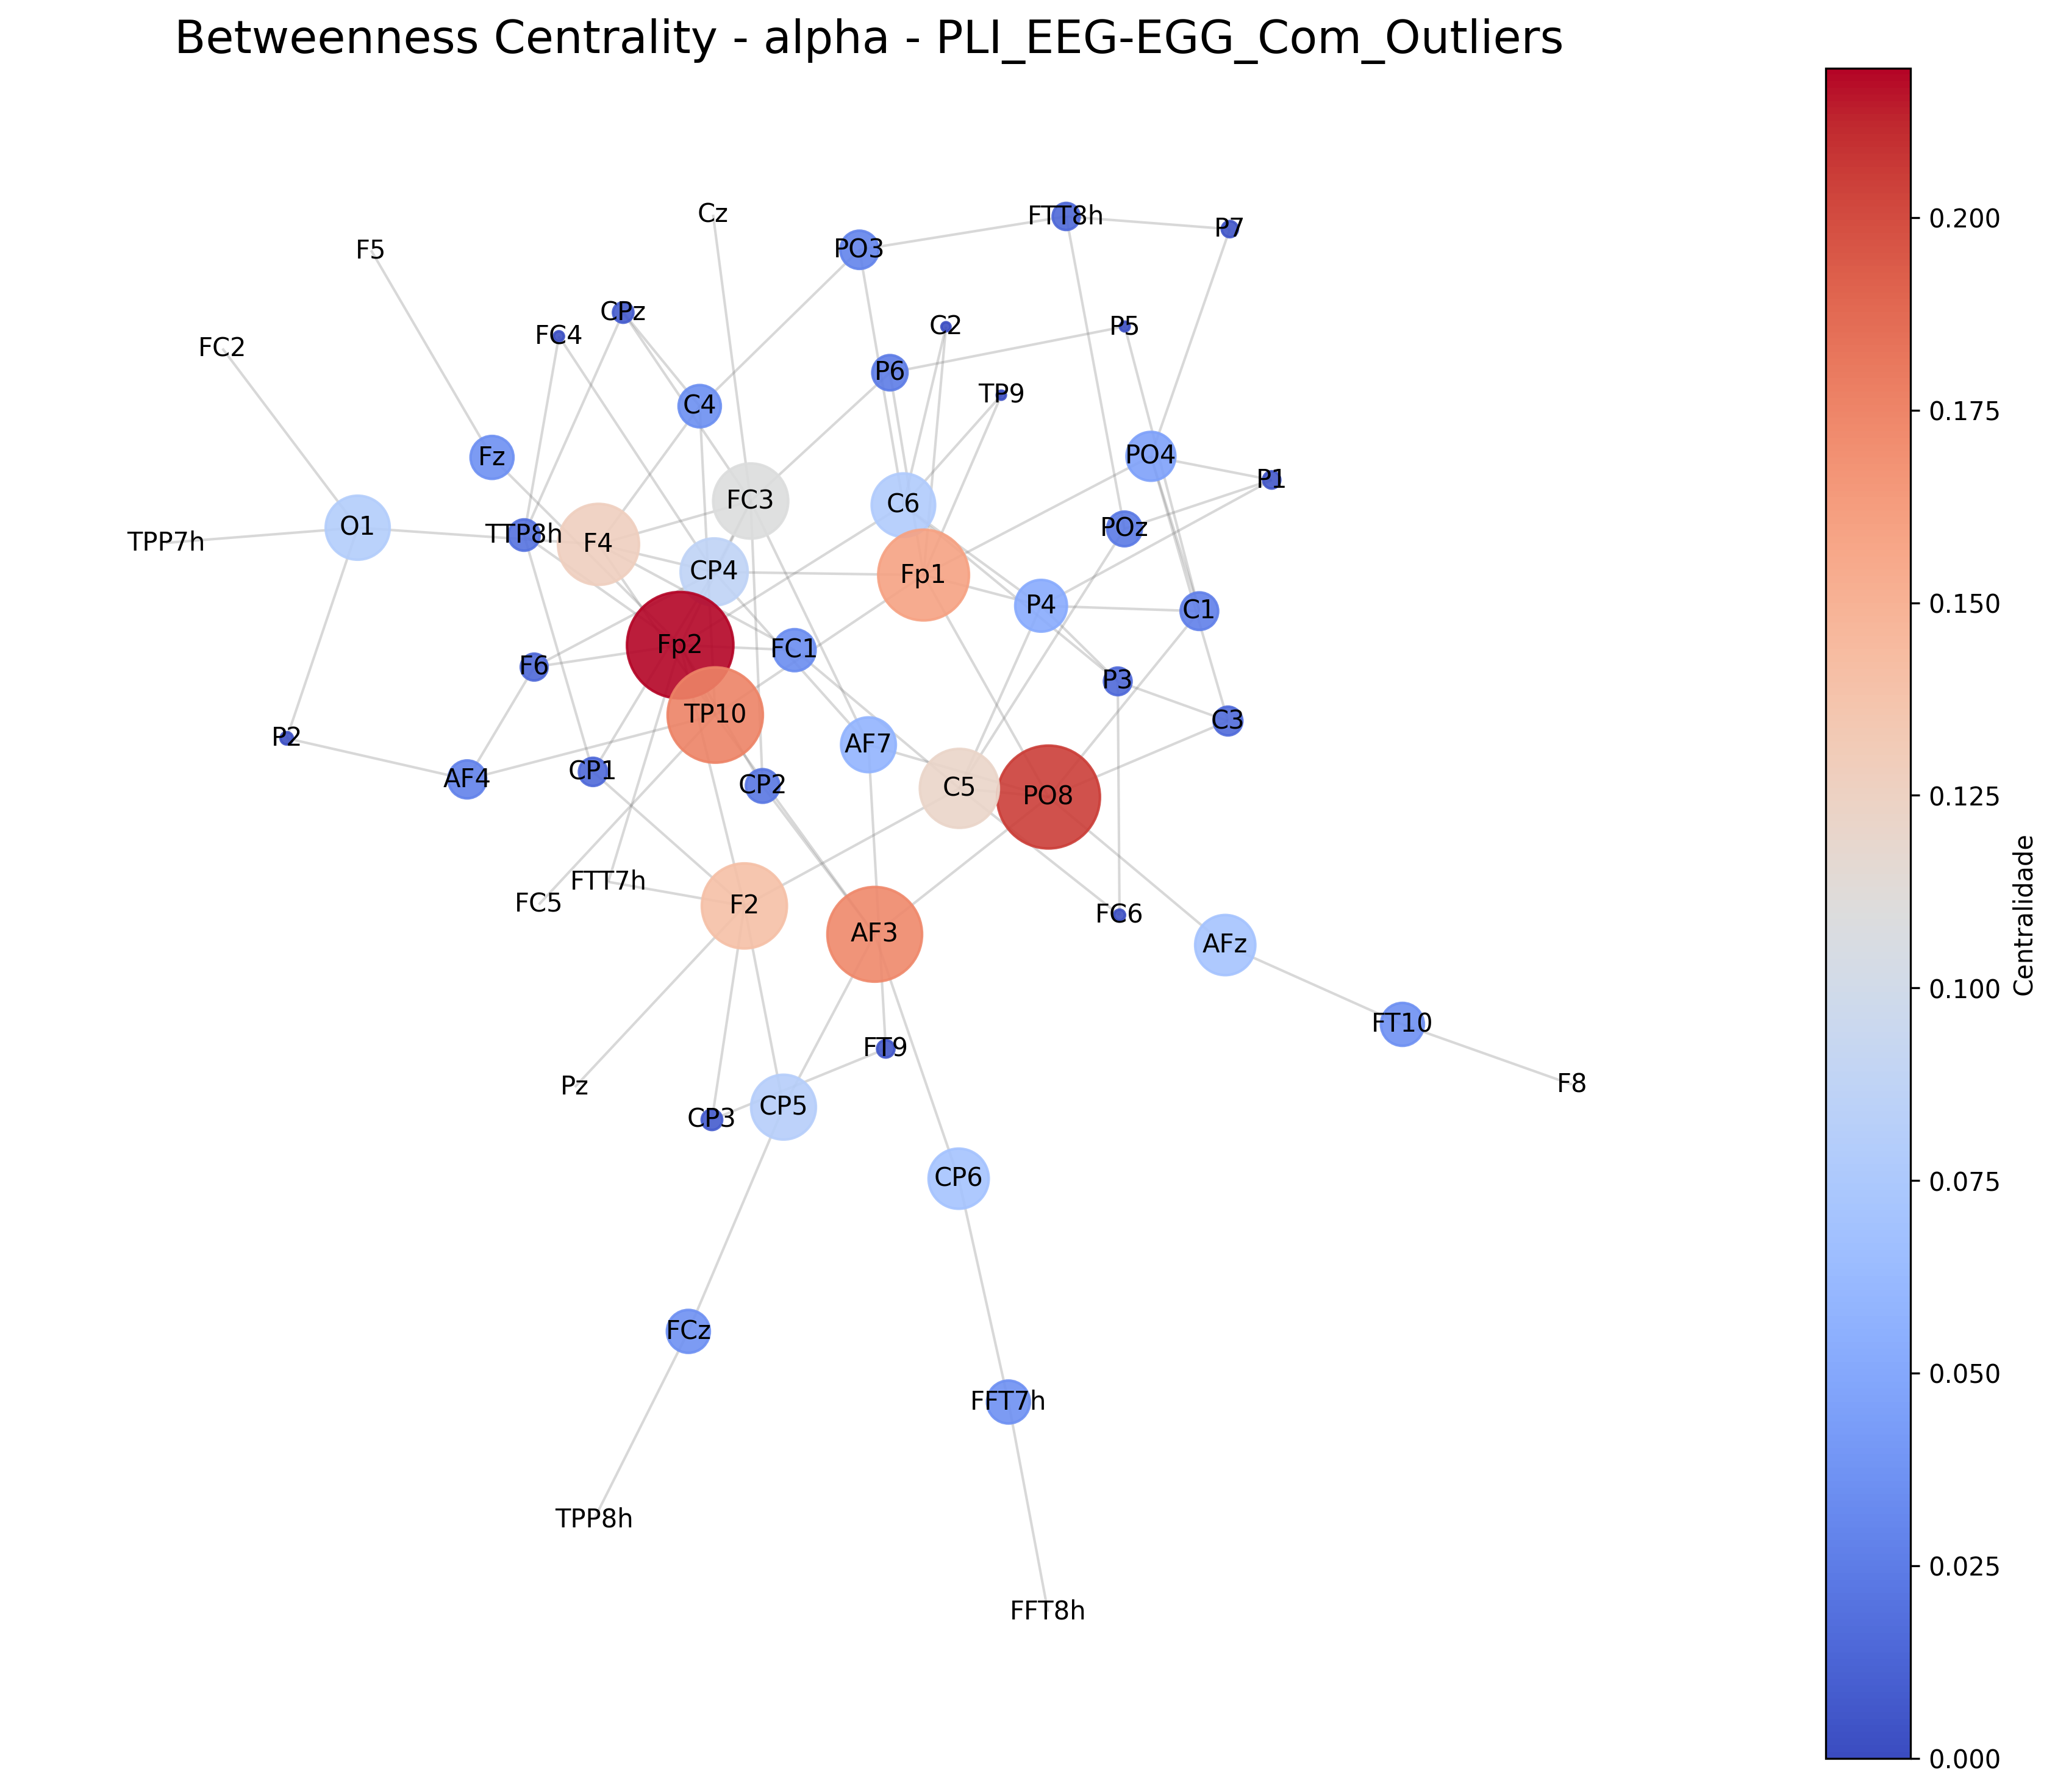
\includegraphics[width=0.45\textwidth]{figs/7_bootstrap_results_analysis/3_centrality_graphs/Com_Outliers/Betweenness_Centrality__alpha__PLI_EEGEGG_Com_Outliers.png}
    }
    \hfill
    \subfloat[\small \textbf{Sem Outliers:} Hierarquia – 1. \textbf{Fp2}; 2. \textbf{PO8, C6, F4, O1}; 3. \textbf{Fp1, TP9}; 4. \textbf{AF3, FC3, F2, TP10}.]{%
        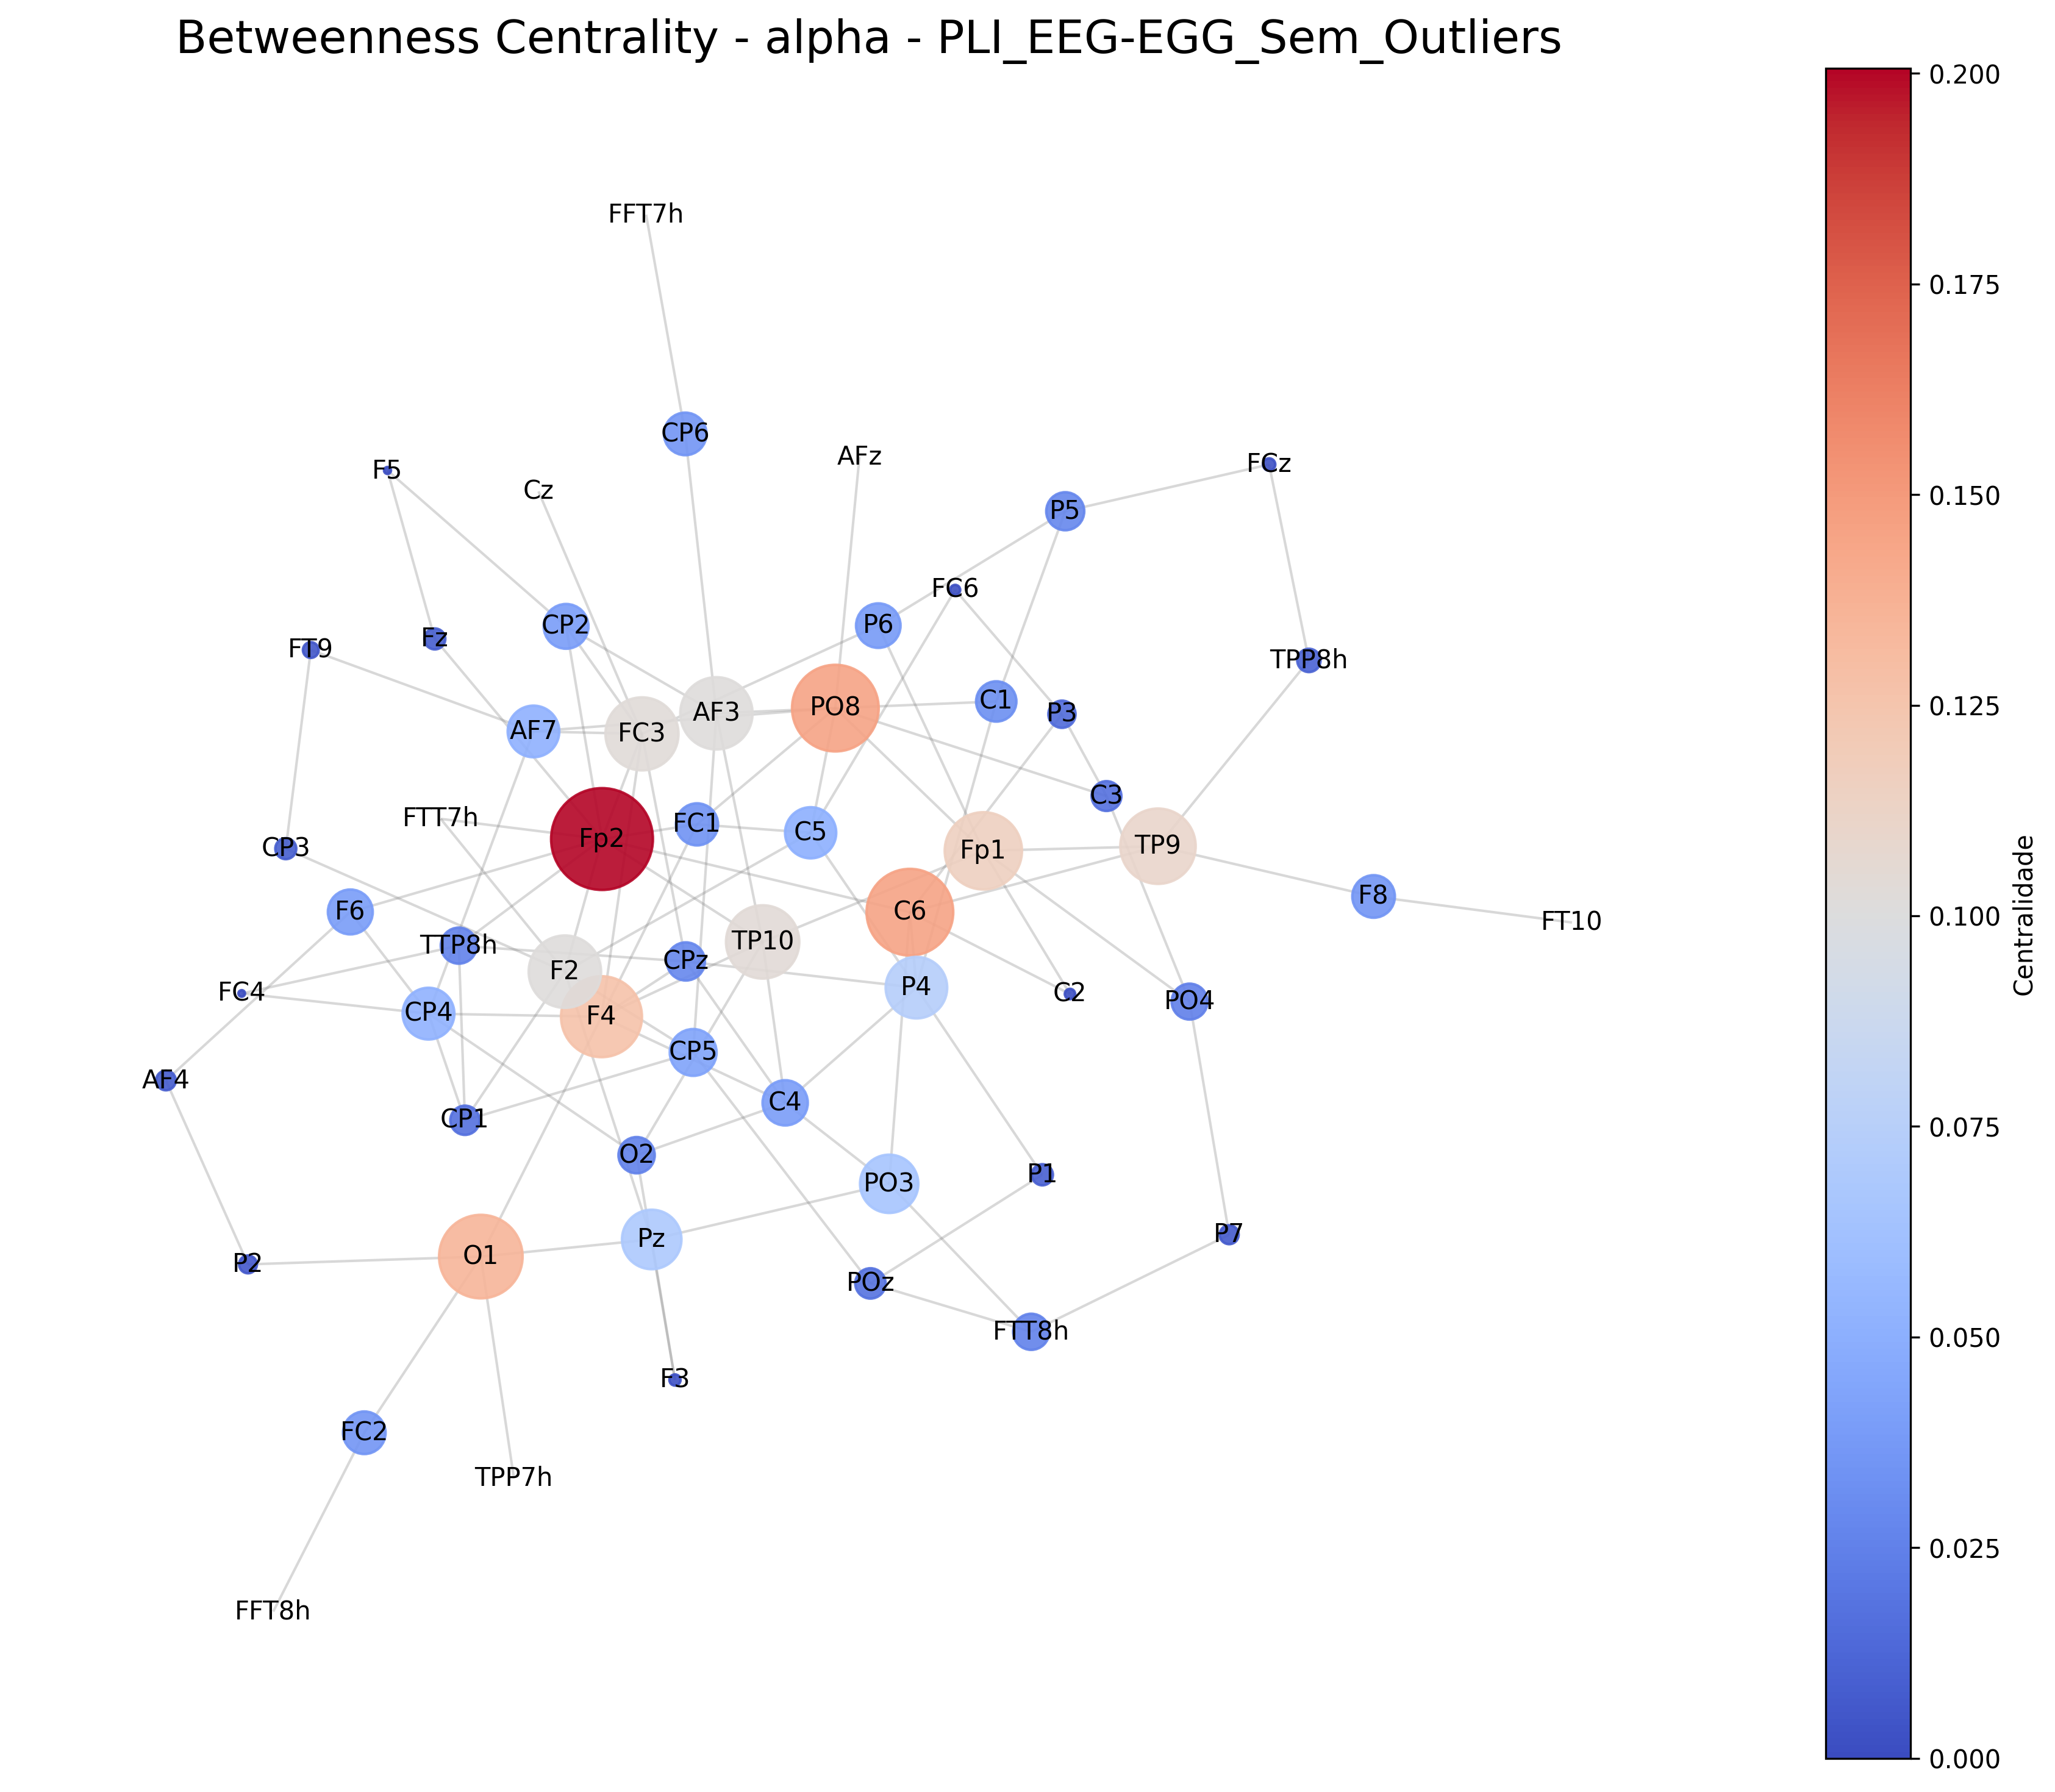
\includegraphics[width=0.45\textwidth]{figs/7_bootstrap_results_analysis/3_centrality_graphs/Sem_Outliers/Betweenness_Centrality__alpha__PLI_EEGEGG_Sem_Outliers.png}
    }
    \caption{\small \textbf{Betweenness Centrality – Banda Alpha (8--13 Hz):} A importância dos canais na mediação dos caminhos da rede é destacada pelos nós com cores mais quentes (vermelho intenso) e maiores tamanhos.}
    \label{fig:betweenness_alpha}
\end{figure}

\subsubsection{Degree Centrality}
\begin{figure}[H]
    \centering
    \subfloat[\small \textbf{Com Outliers:} Hierarquia – 1. \textbf{Fp2}; 2. \textbf{FC3, Fp1}; 3. \textbf{CP4, TP10, PO8, F2}; 4. \textbf{F4, C6, P4, C5}.]{%
        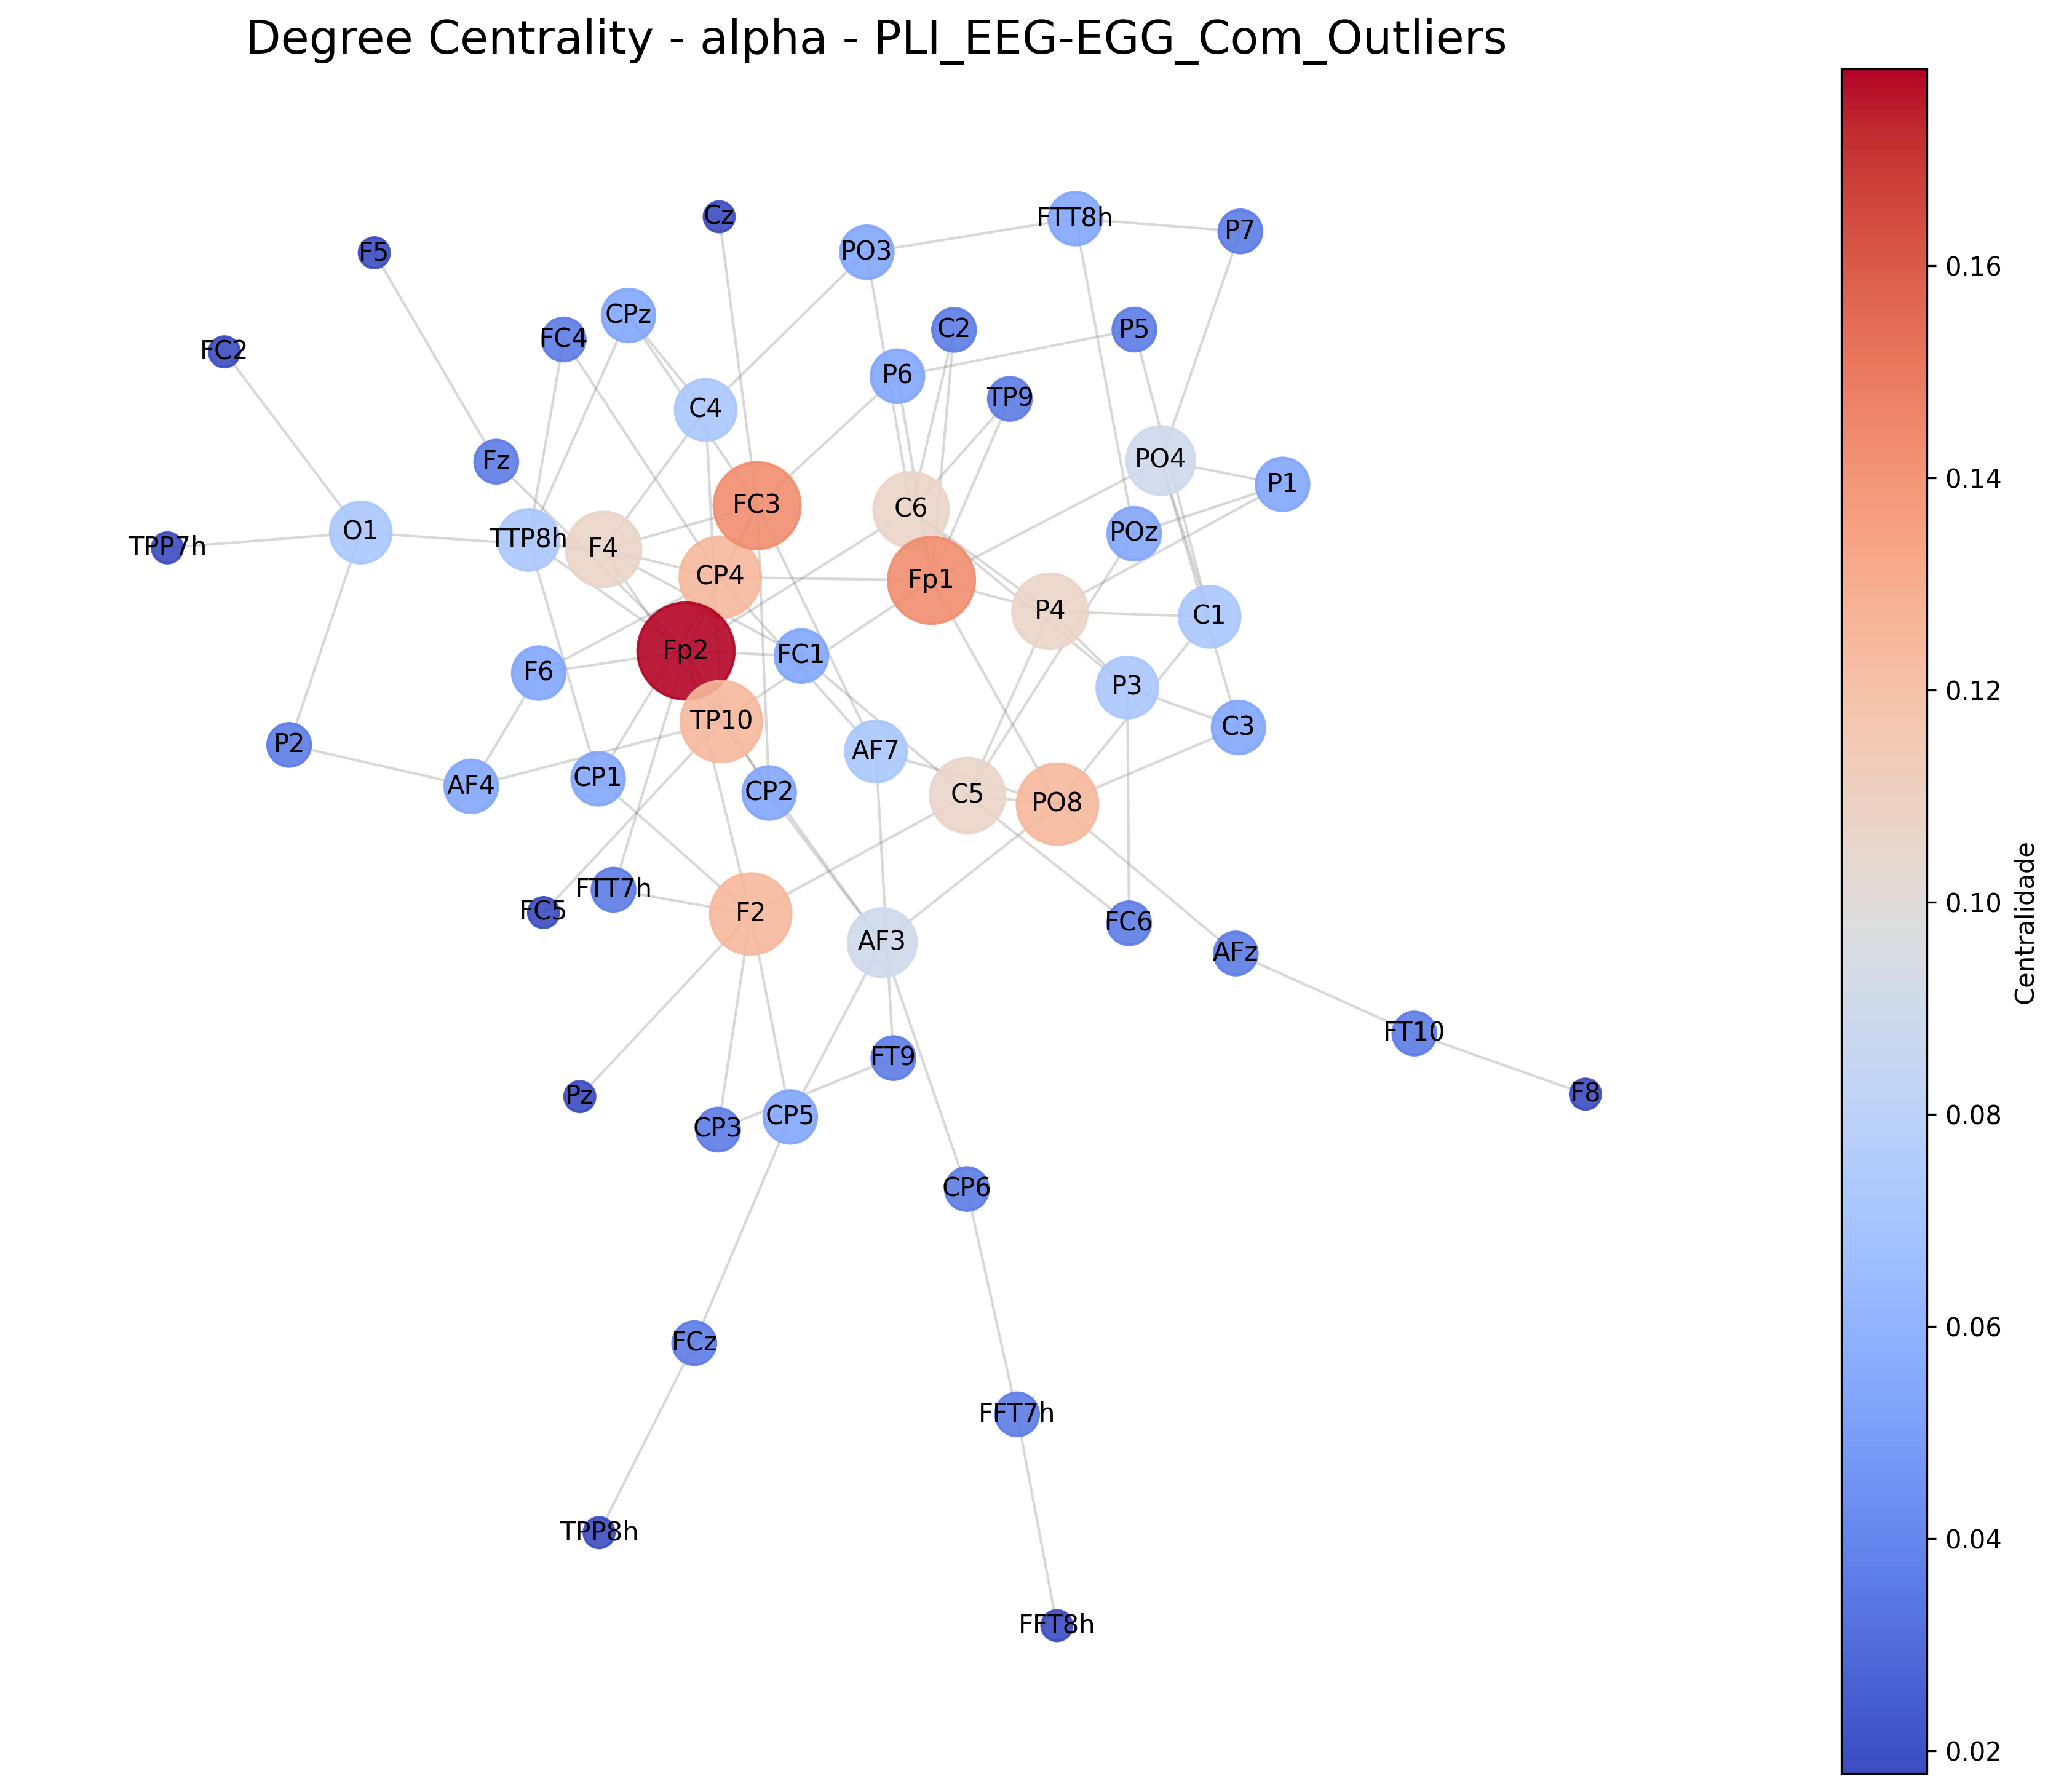
\includegraphics[width=0.45\textwidth]{figs/7_bootstrap_results_analysis/3_centrality_graphs/Com_Outliers/Degree_Centrality__alpha__PLI_EEGEGG_Com_Outliers.png}
    }
    \hfill
    \subfloat[\small \textbf{Sem Outliers:} Hierarquia – 1. \textbf{Fp2}; 2. \textbf{PO8}; 3. \textbf{FC3, F2, F4}; 4. \textbf{C6, Fp1, P4, C4, CP4}.]{%
        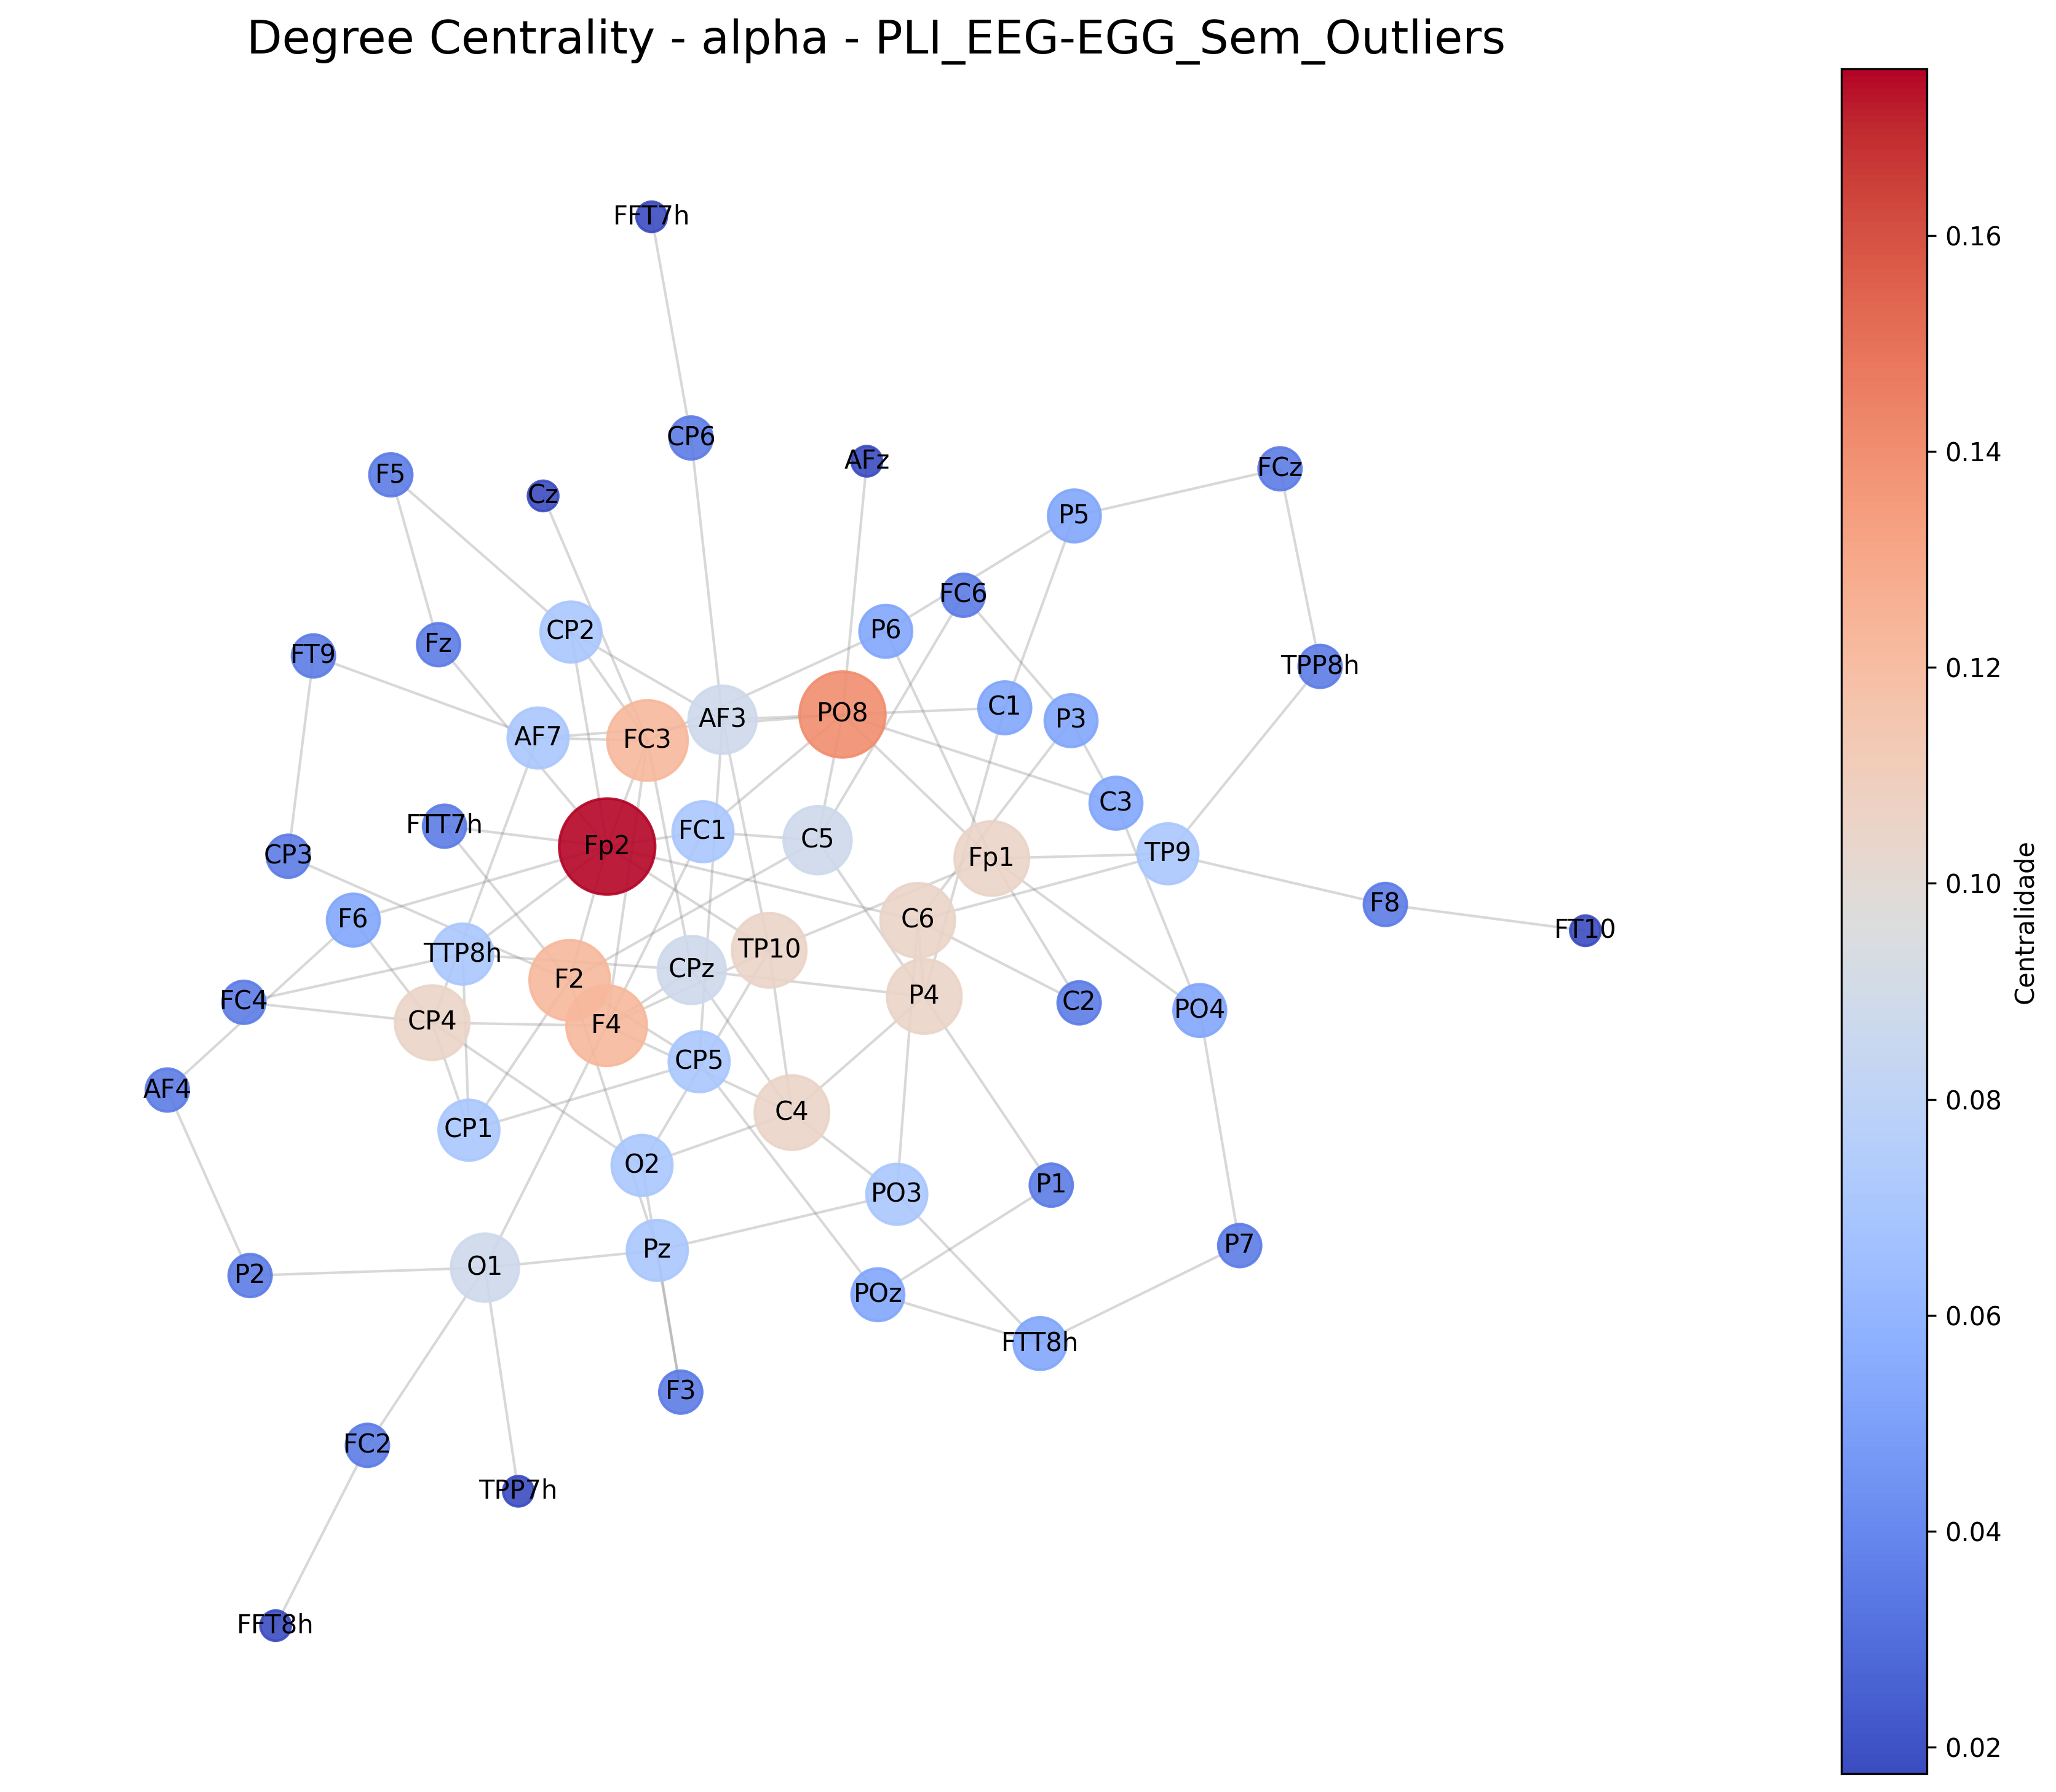
\includegraphics[width=0.45\textwidth]{figs/7_bootstrap_results_analysis/3_centrality_graphs/Sem_Outliers/Degree_Centrality__alpha__PLI_EEGEGG_Sem_Outliers.png}
    }
    \caption{\small \textbf{Degree Centrality – Banda Alpha (8--13 Hz):} Os nós com maior número de conexões diretas aparecem destacados, evidenciando a hierarquia dos canais na rede.}
    \label{fig:degree_alpha}
\end{figure}

\subsubsection{Eigenvector Centrality}
\begin{figure}[H]
    \centering
    \subfloat[\small \textbf{Com Outliers:} Hierarquia – 1. \textbf{Fp2}; 2. \textbf{FC3}; 3. \textbf{CP4, F4, TP10, Fp1}; 4. \textbf{PO8}.]{%
        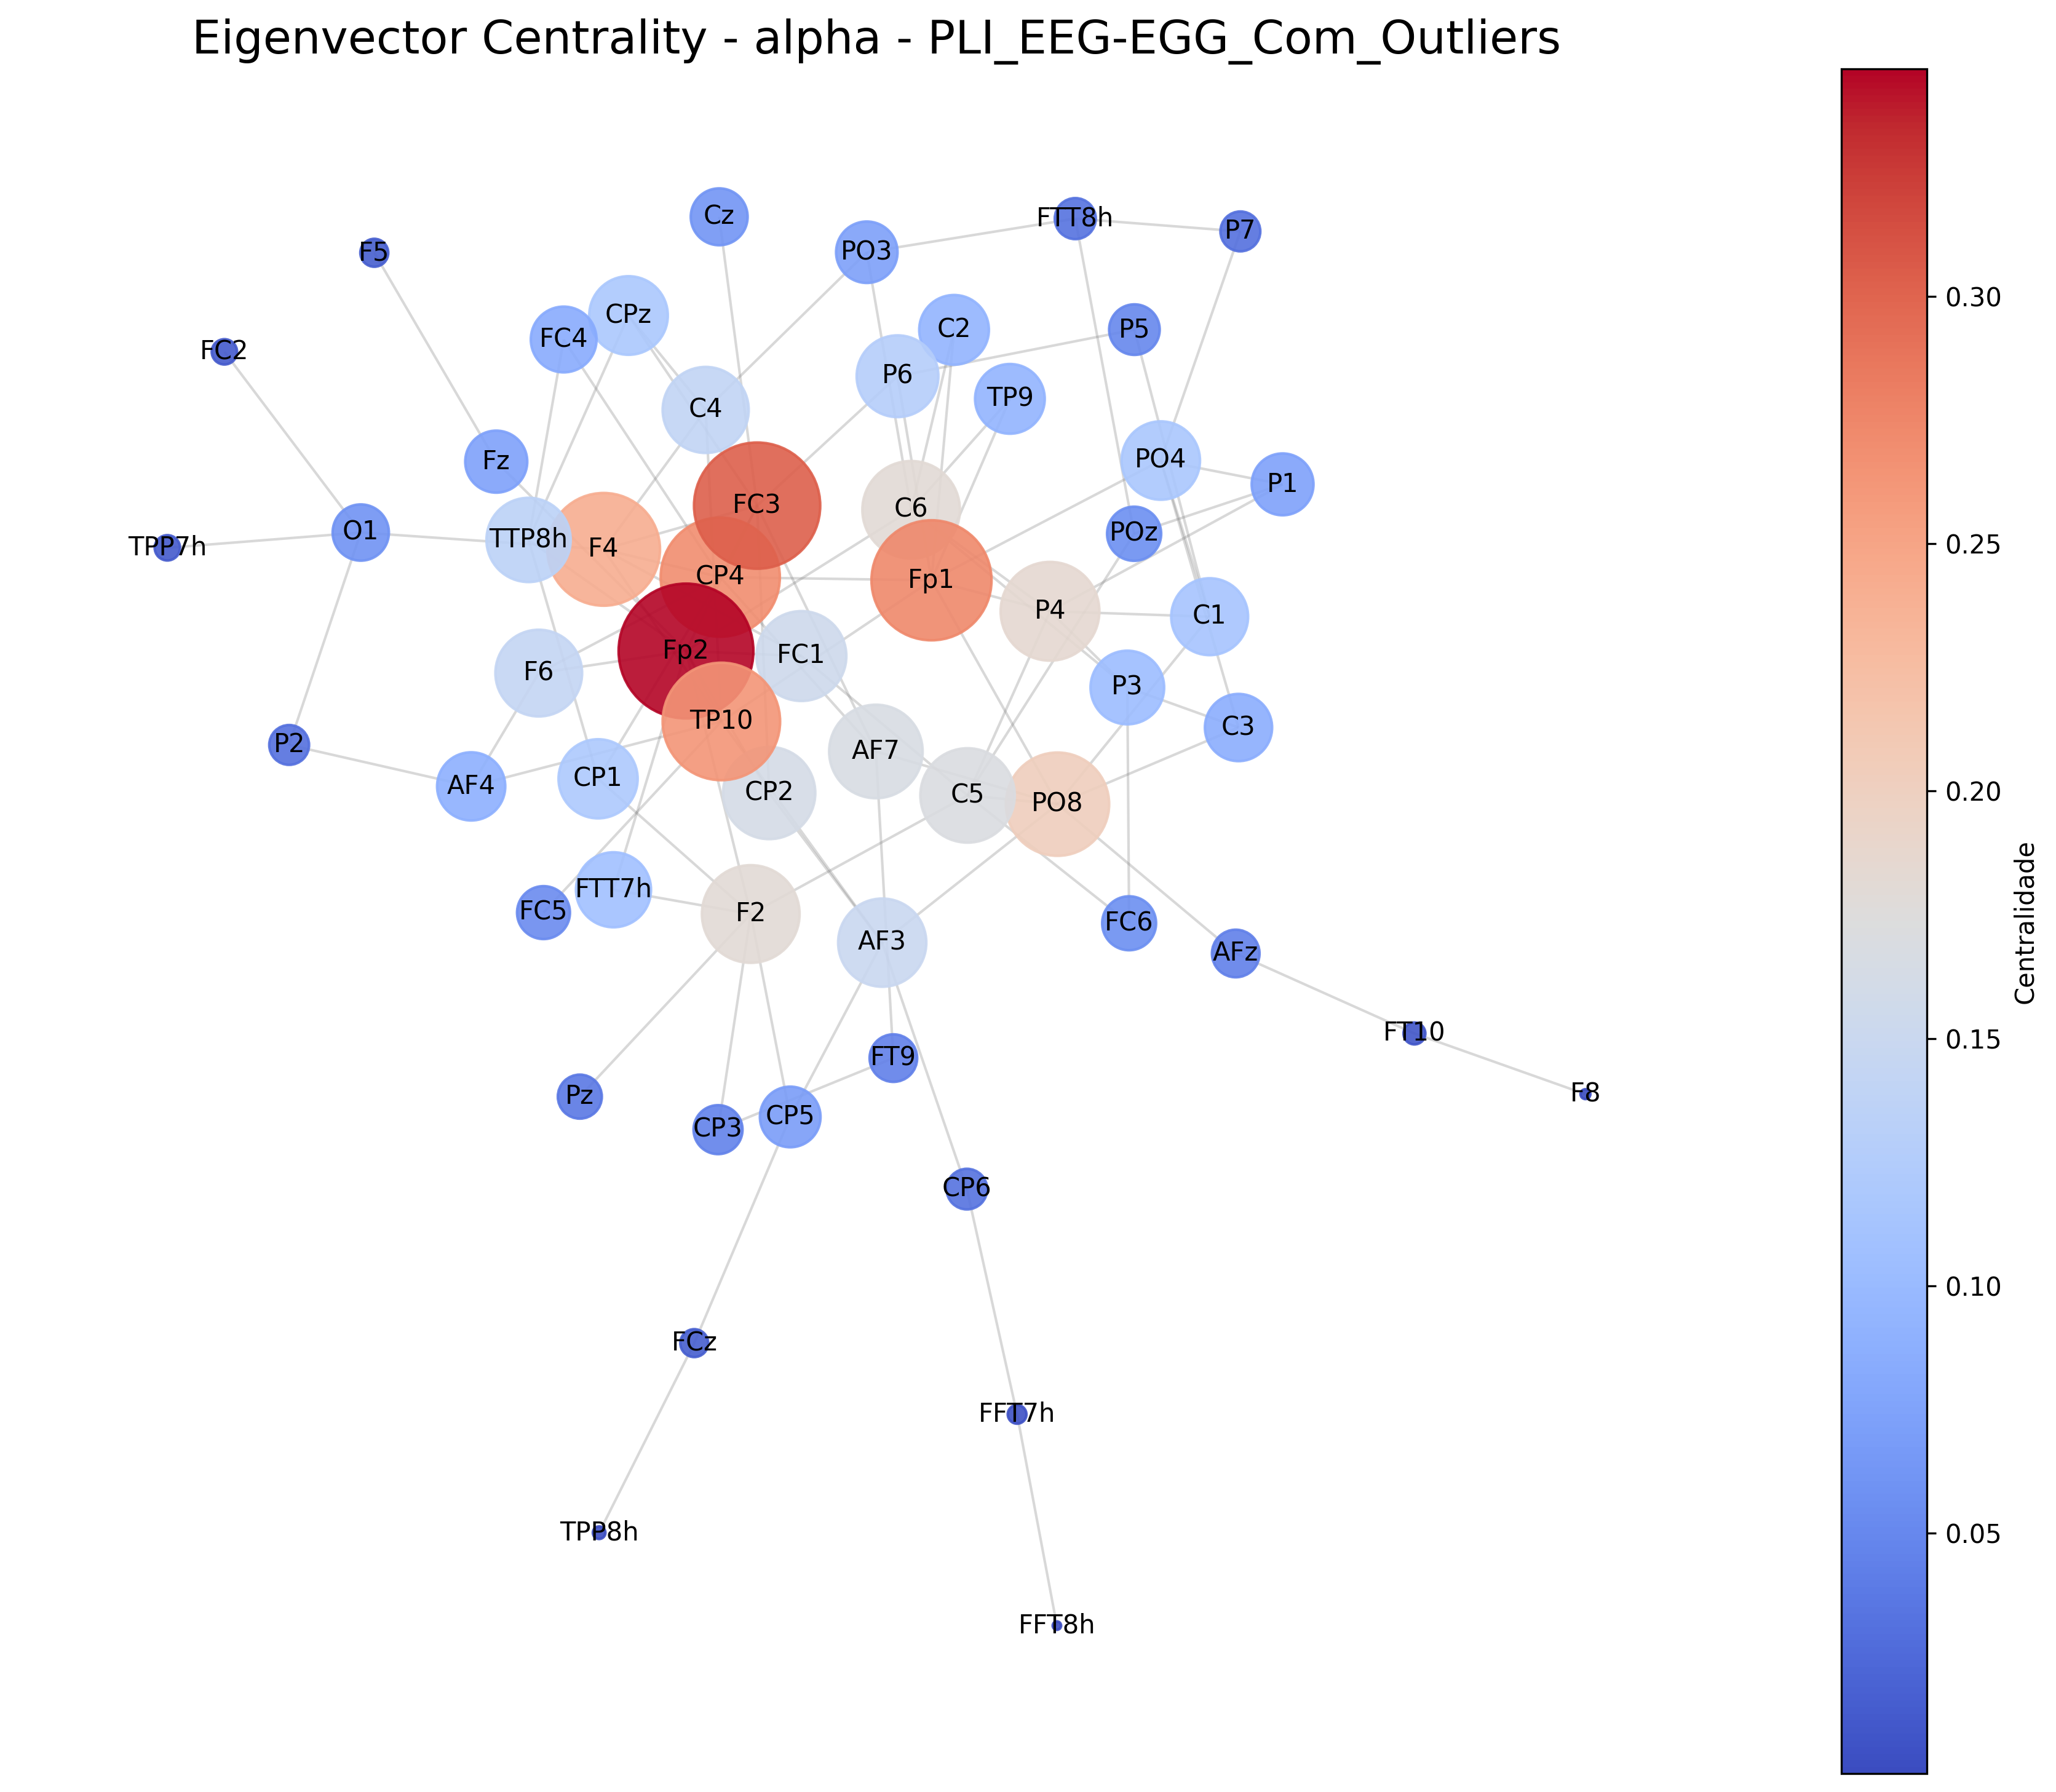
\includegraphics[width=0.45\textwidth]{figs/7_bootstrap_results_analysis/3_centrality_graphs/Com_Outliers/Eigenvector_Centrality__alpha__PLI_EEGEGG_Com_Outliers.png}
    }
    \hfill
    \subfloat[\small \textbf{Sem Outliers:} Hierarquia – 1. \textbf{Fp2}; 2. \textbf{F4}; 3. \textbf{FC3, TP10}; 4. \textbf{Cpz, C4}; 5. \textbf{PO8, P4, FC1, F2, P4}.]{%
        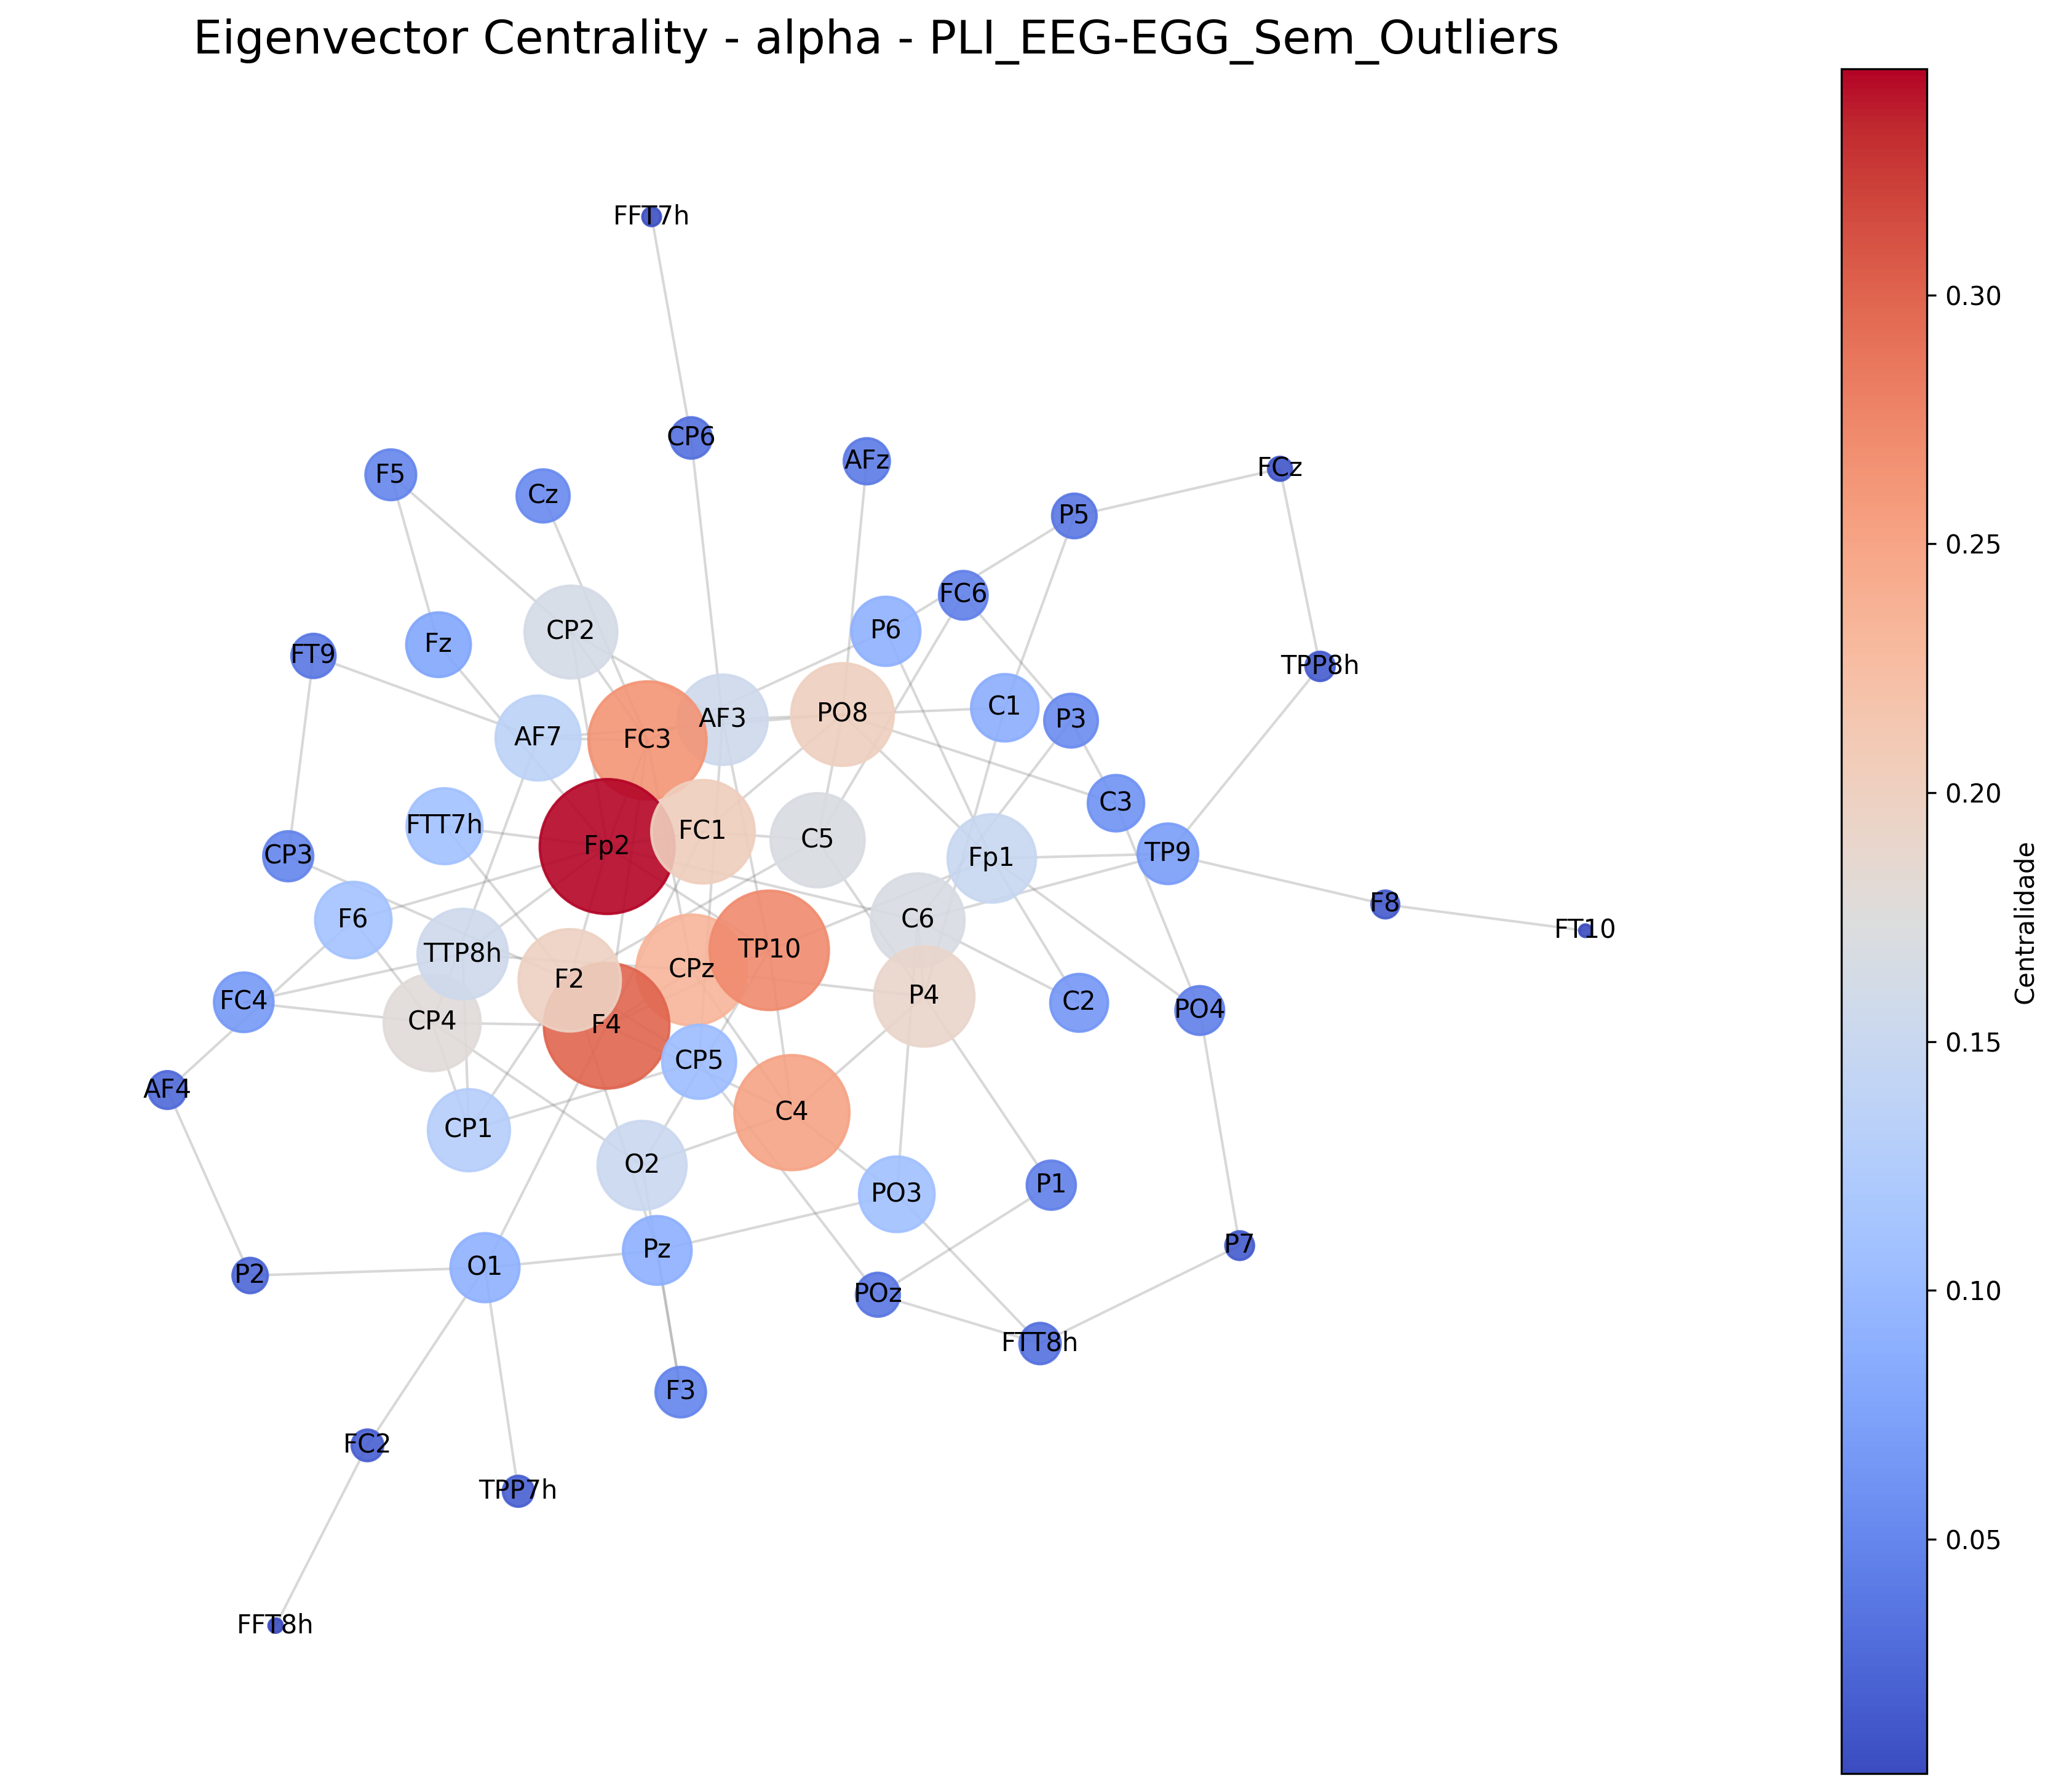
\includegraphics[width=0.45\textwidth]{figs/7_bootstrap_results_analysis/3_centrality_graphs/Sem_Outliers/Eigenvector_Centrality__alpha__PLI_EEGEGG_Sem_Outliers.png}
    }
    \caption{\small \textbf{Eigenvector Centrality – Banda Alpha (8--13 Hz):} A influência dos canais é demonstrada pela hierarquia dos nós, com os valores mais elevados destacados em tons intensos.}
    \label{fig:eigenvector_alpha}
\end{figure}

\subsection{Banda Beta (13--30 Hz)}
\subsubsection{Betweenness Centrality}
\begin{figure}[H]
    \centering
    \subfloat[\small \textbf{Com Outliers:} Hierarquia – 1. \textbf{CP5, F5}; 2. \textbf{CP1}; 3. \textbf{F2, POz}; 4. \textbf{TPP7h}.]{%
        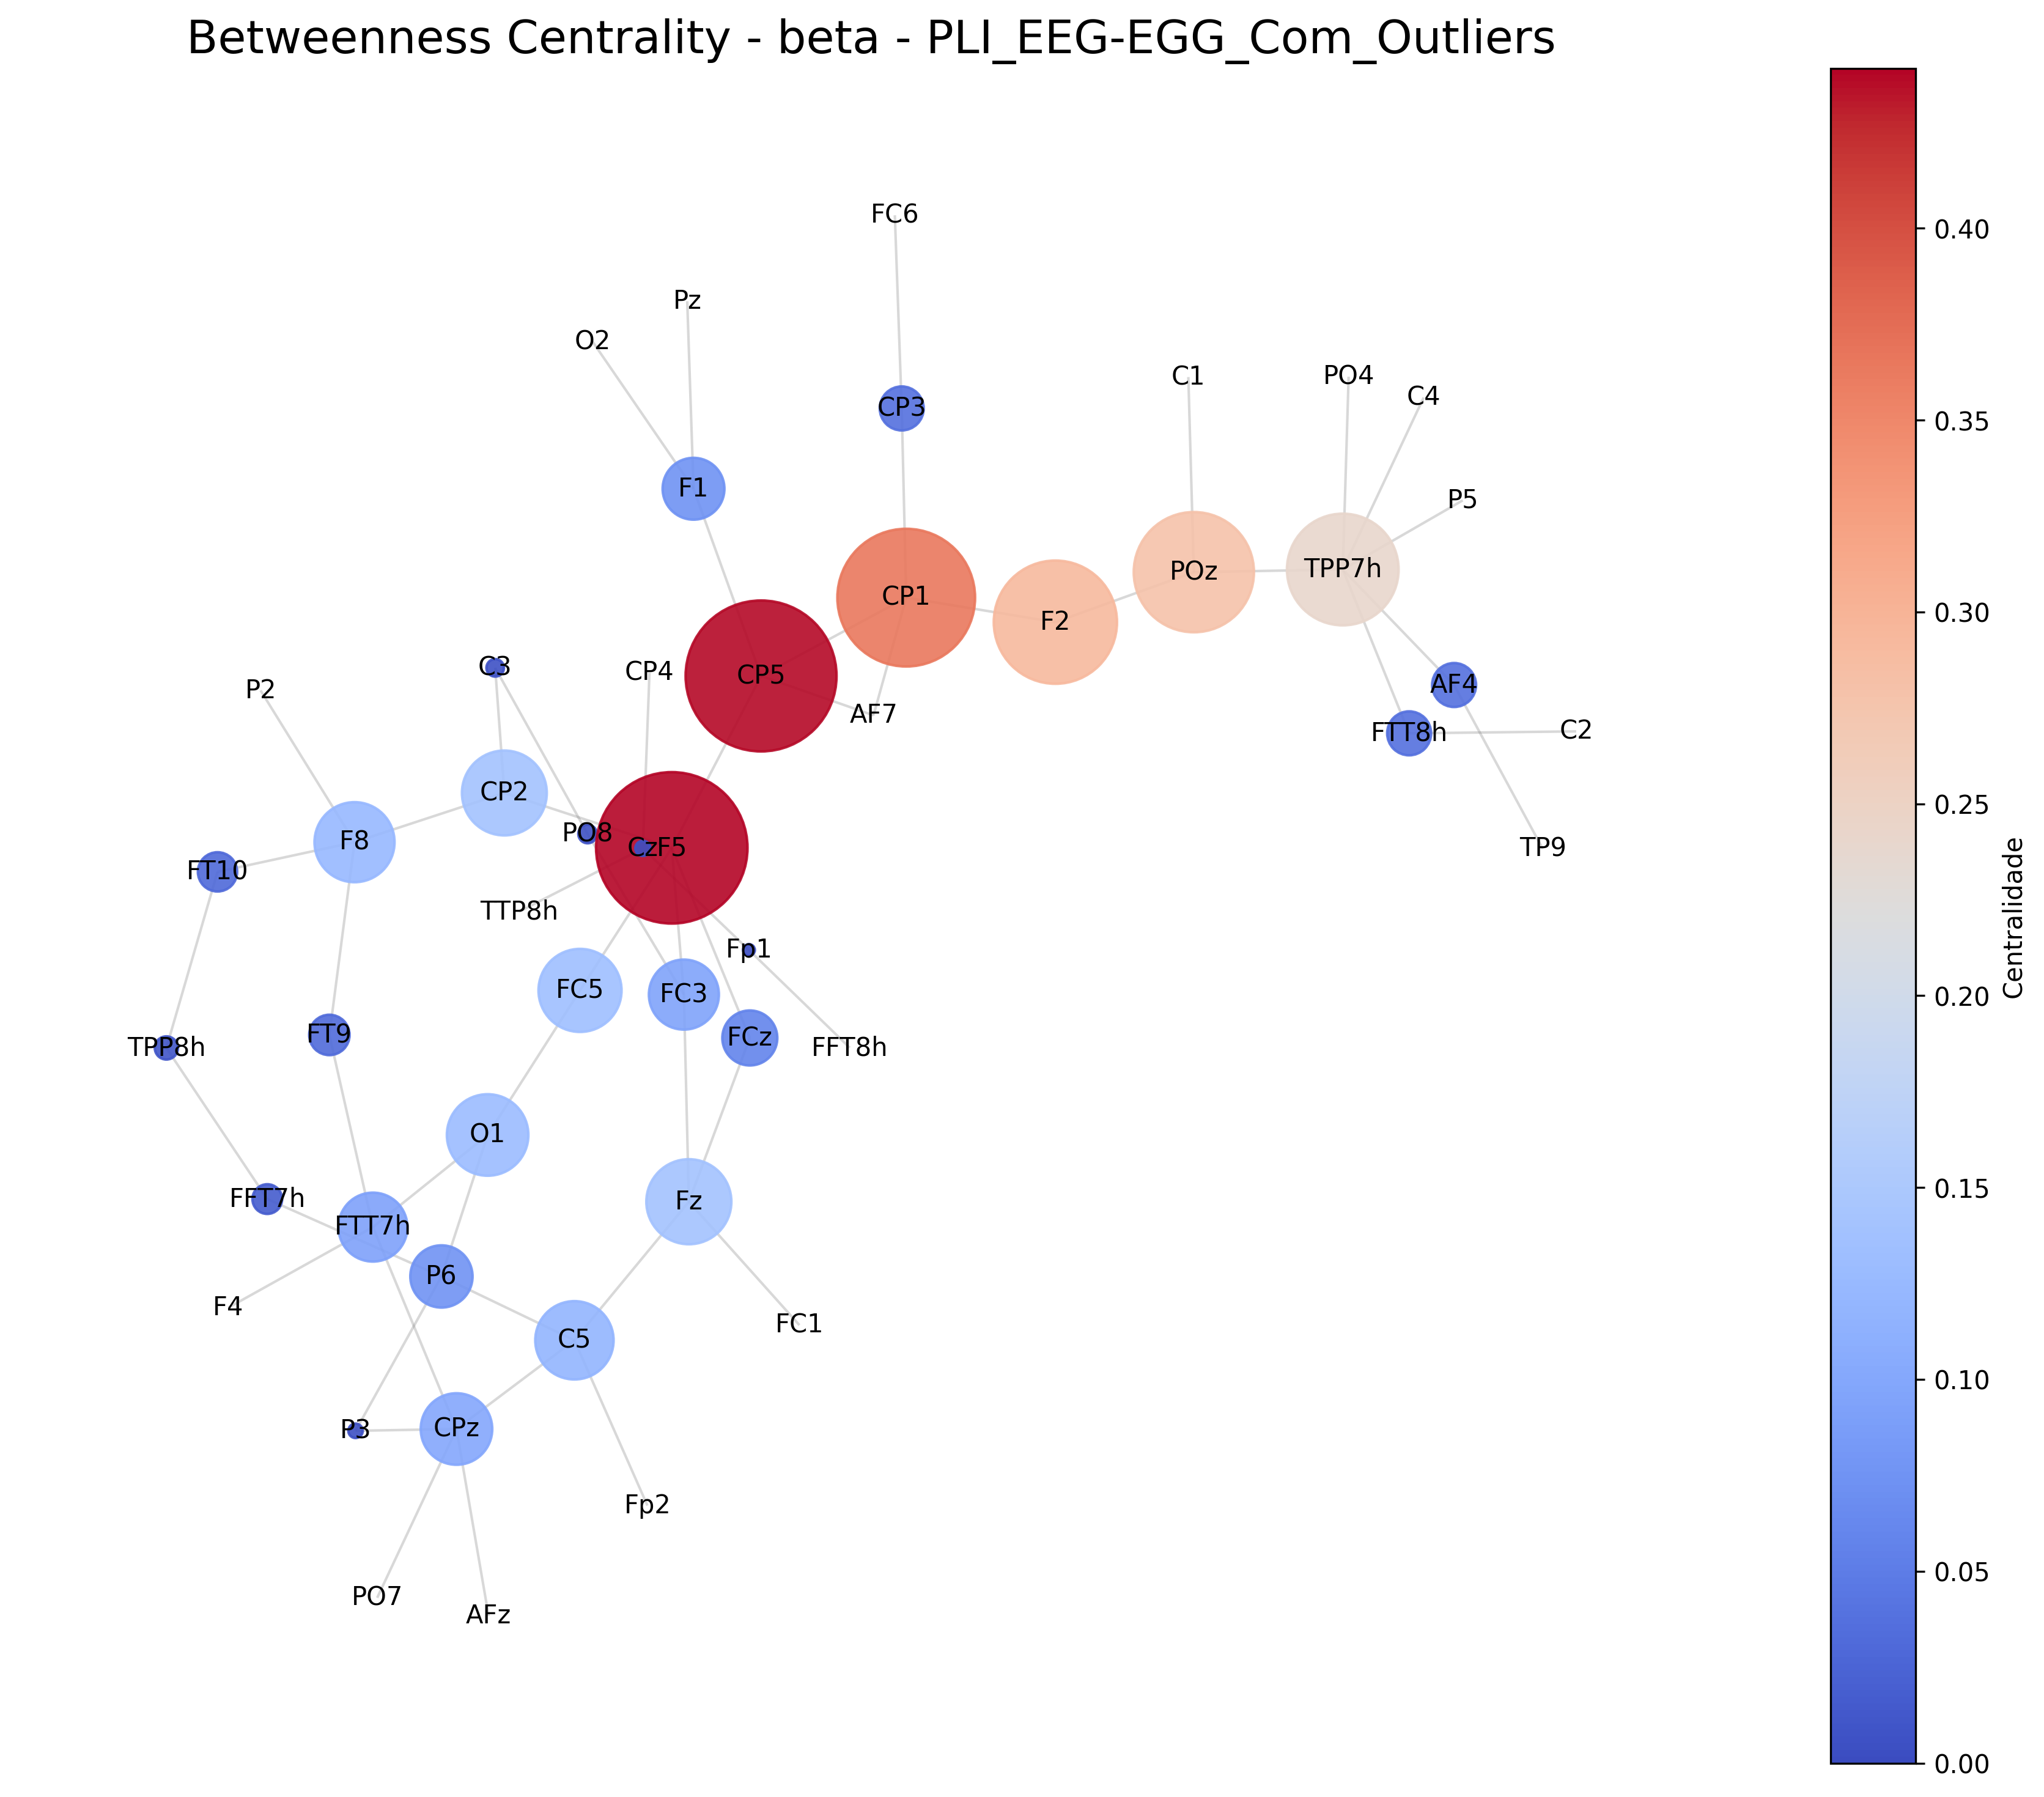
\includegraphics[width=0.45\textwidth]{figs/7_bootstrap_results_analysis/3_centrality_graphs/Com_Outliers/Betweenness_Centrality__beta__PLI_EEGEGG_Com_Outliers.png}
    }
    \hfill
    \subfloat[\small \textbf{Sem Outliers:} Hierarquia – 1. \textbf{TPP7h}; 2. \textbf{CP5, F5, CP2}; 3. \textbf{FFT7h}; 4. \textbf{TTP8h}; 5. \textbf{CPz}; 6. \textbf{P6}.]{%
        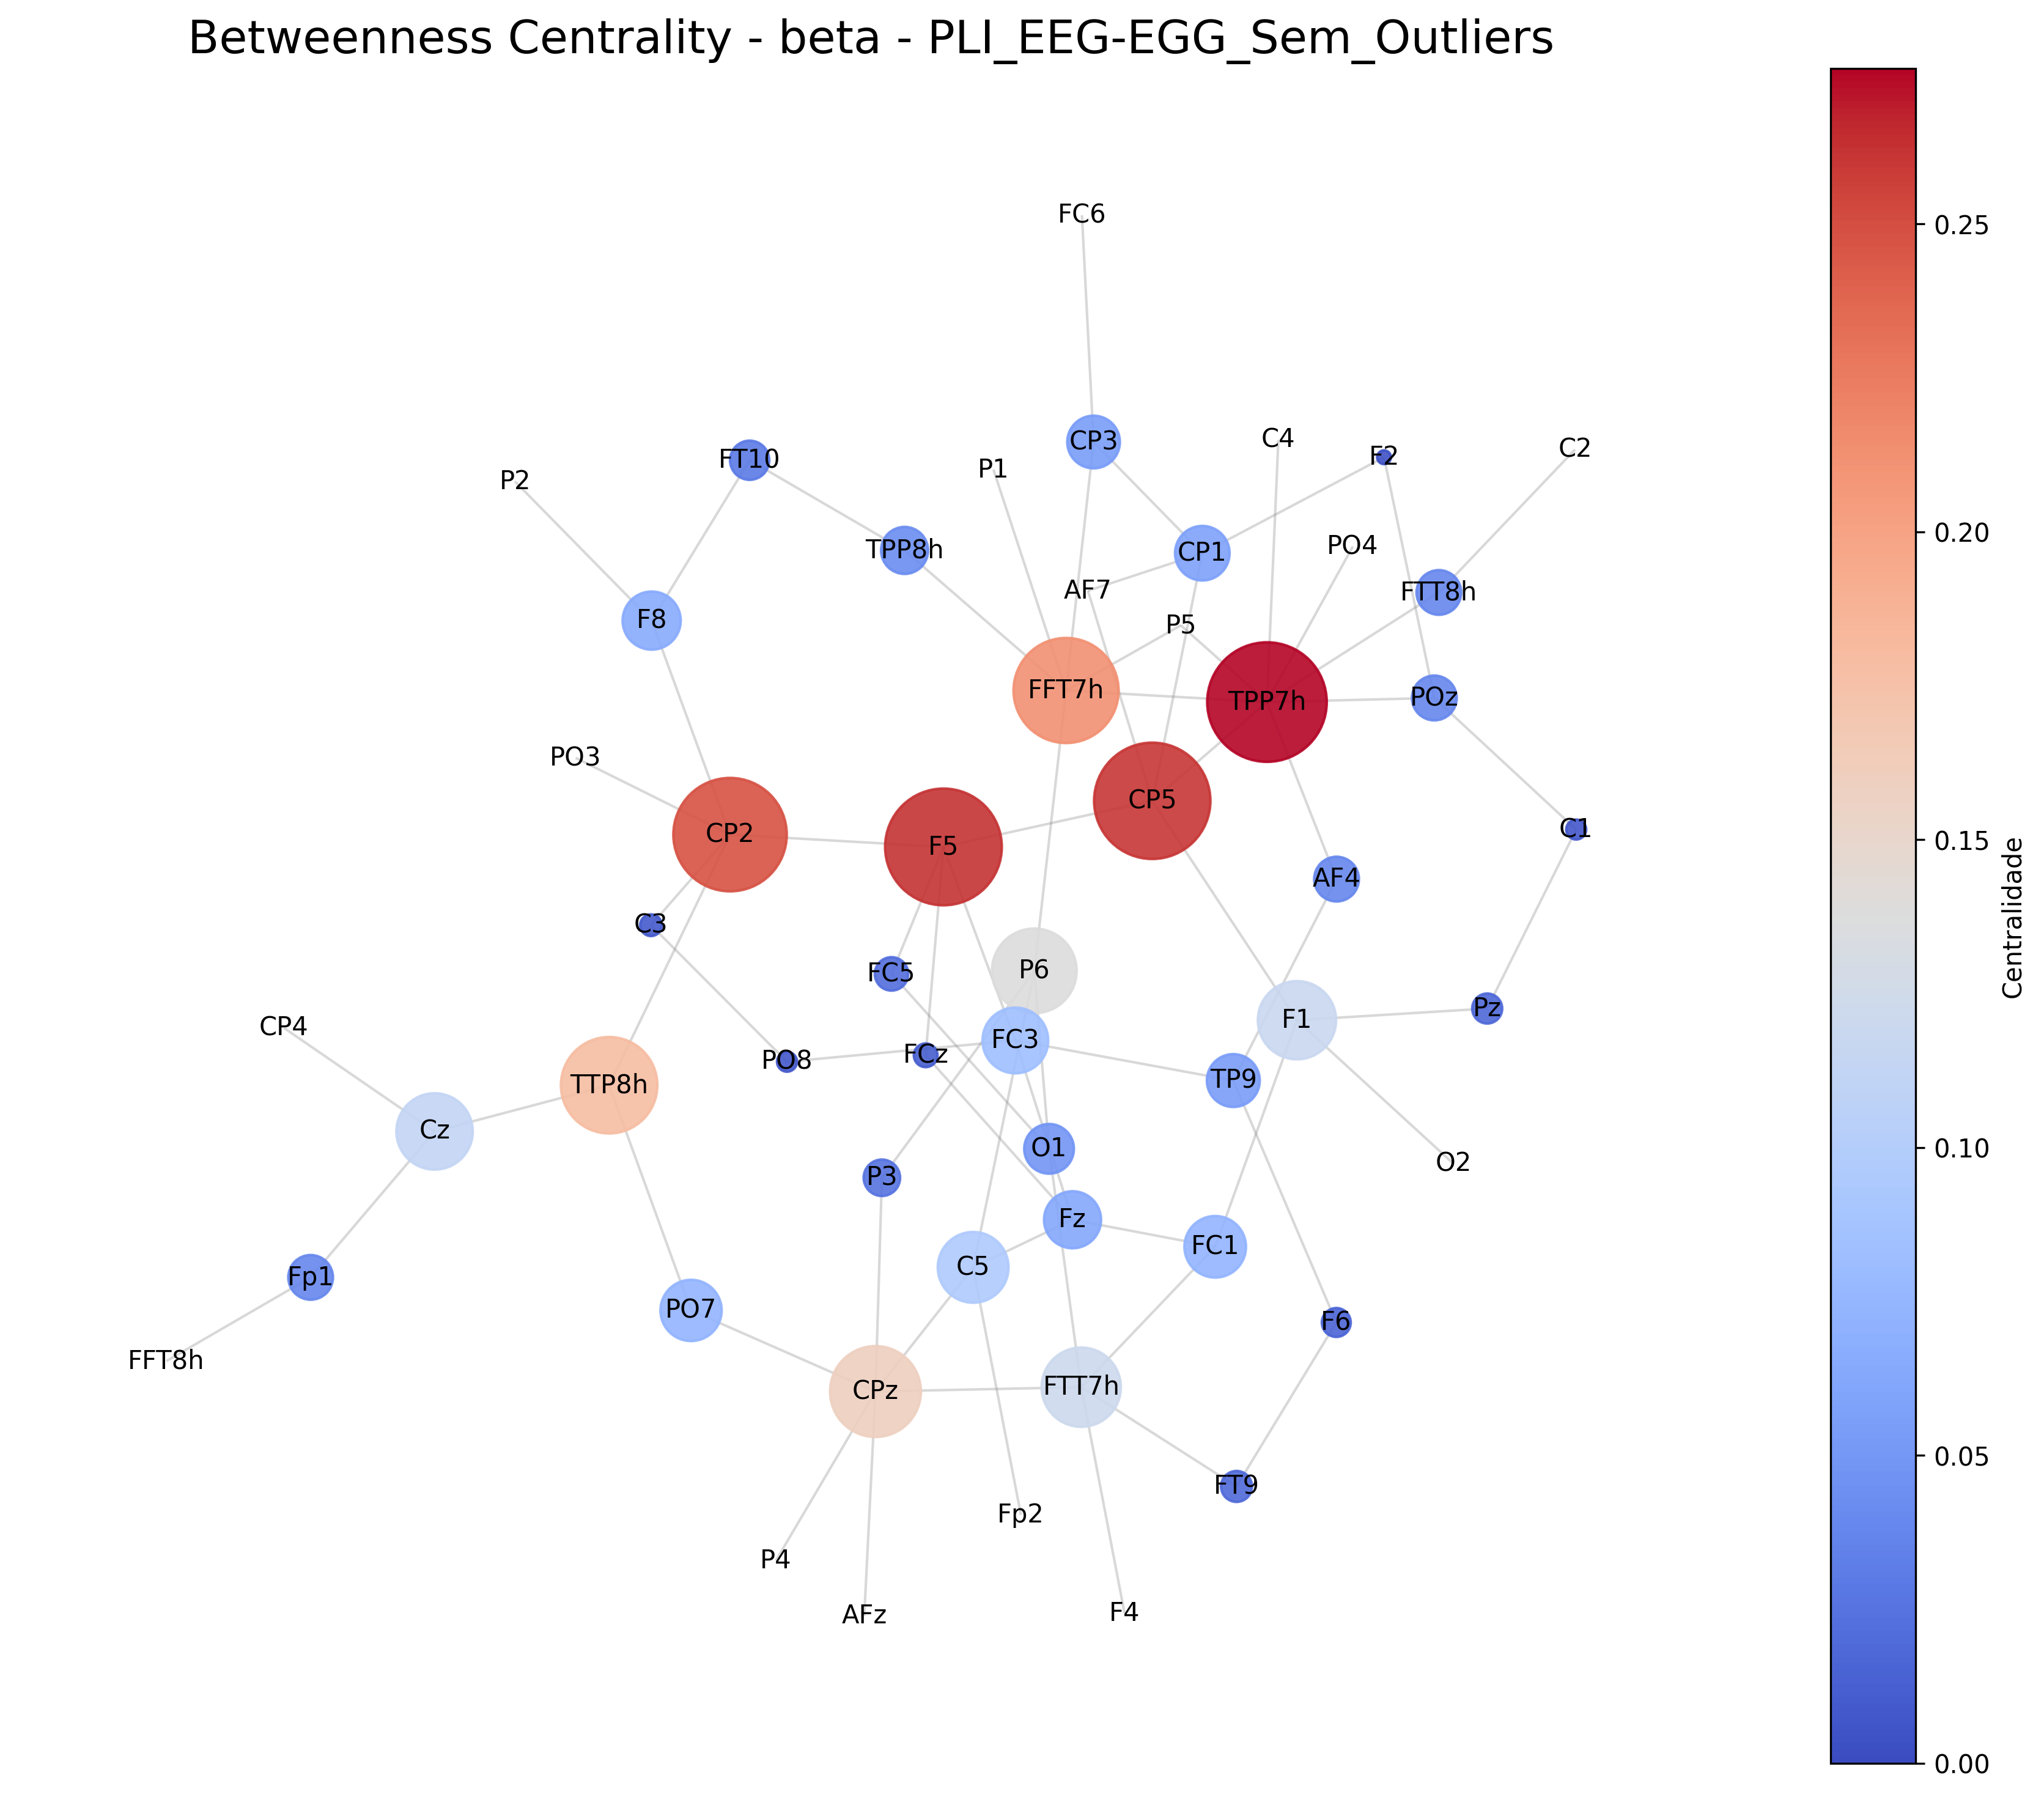
\includegraphics[width=0.45\textwidth]{figs/7_bootstrap_results_analysis/3_centrality_graphs/Sem_Outliers/Betweenness_Centrality__beta__PLI_EEGEGG_Sem_Outliers.png}
    }
    \caption{\small \textbf{Betweenness Centrality – Banda Beta (13--30 Hz):} A rede beta evidencia canais-chave, com destaque para \textbf{TPP7h} na versão sem outliers.}
    \label{fig:betweenness_beta}
\end{figure}

\subsubsection{Degree Centrality}
\begin{figure}[H]
    \centering
    \subfloat[\small \textbf{Com Outliers:} Hierarquia – 1. \textbf{TPP7h}; 2. \textbf{F5, CPz}; 3. \textbf{CP1, CP5, F8, FTT7h, P6, C5, Fz}.]{%
        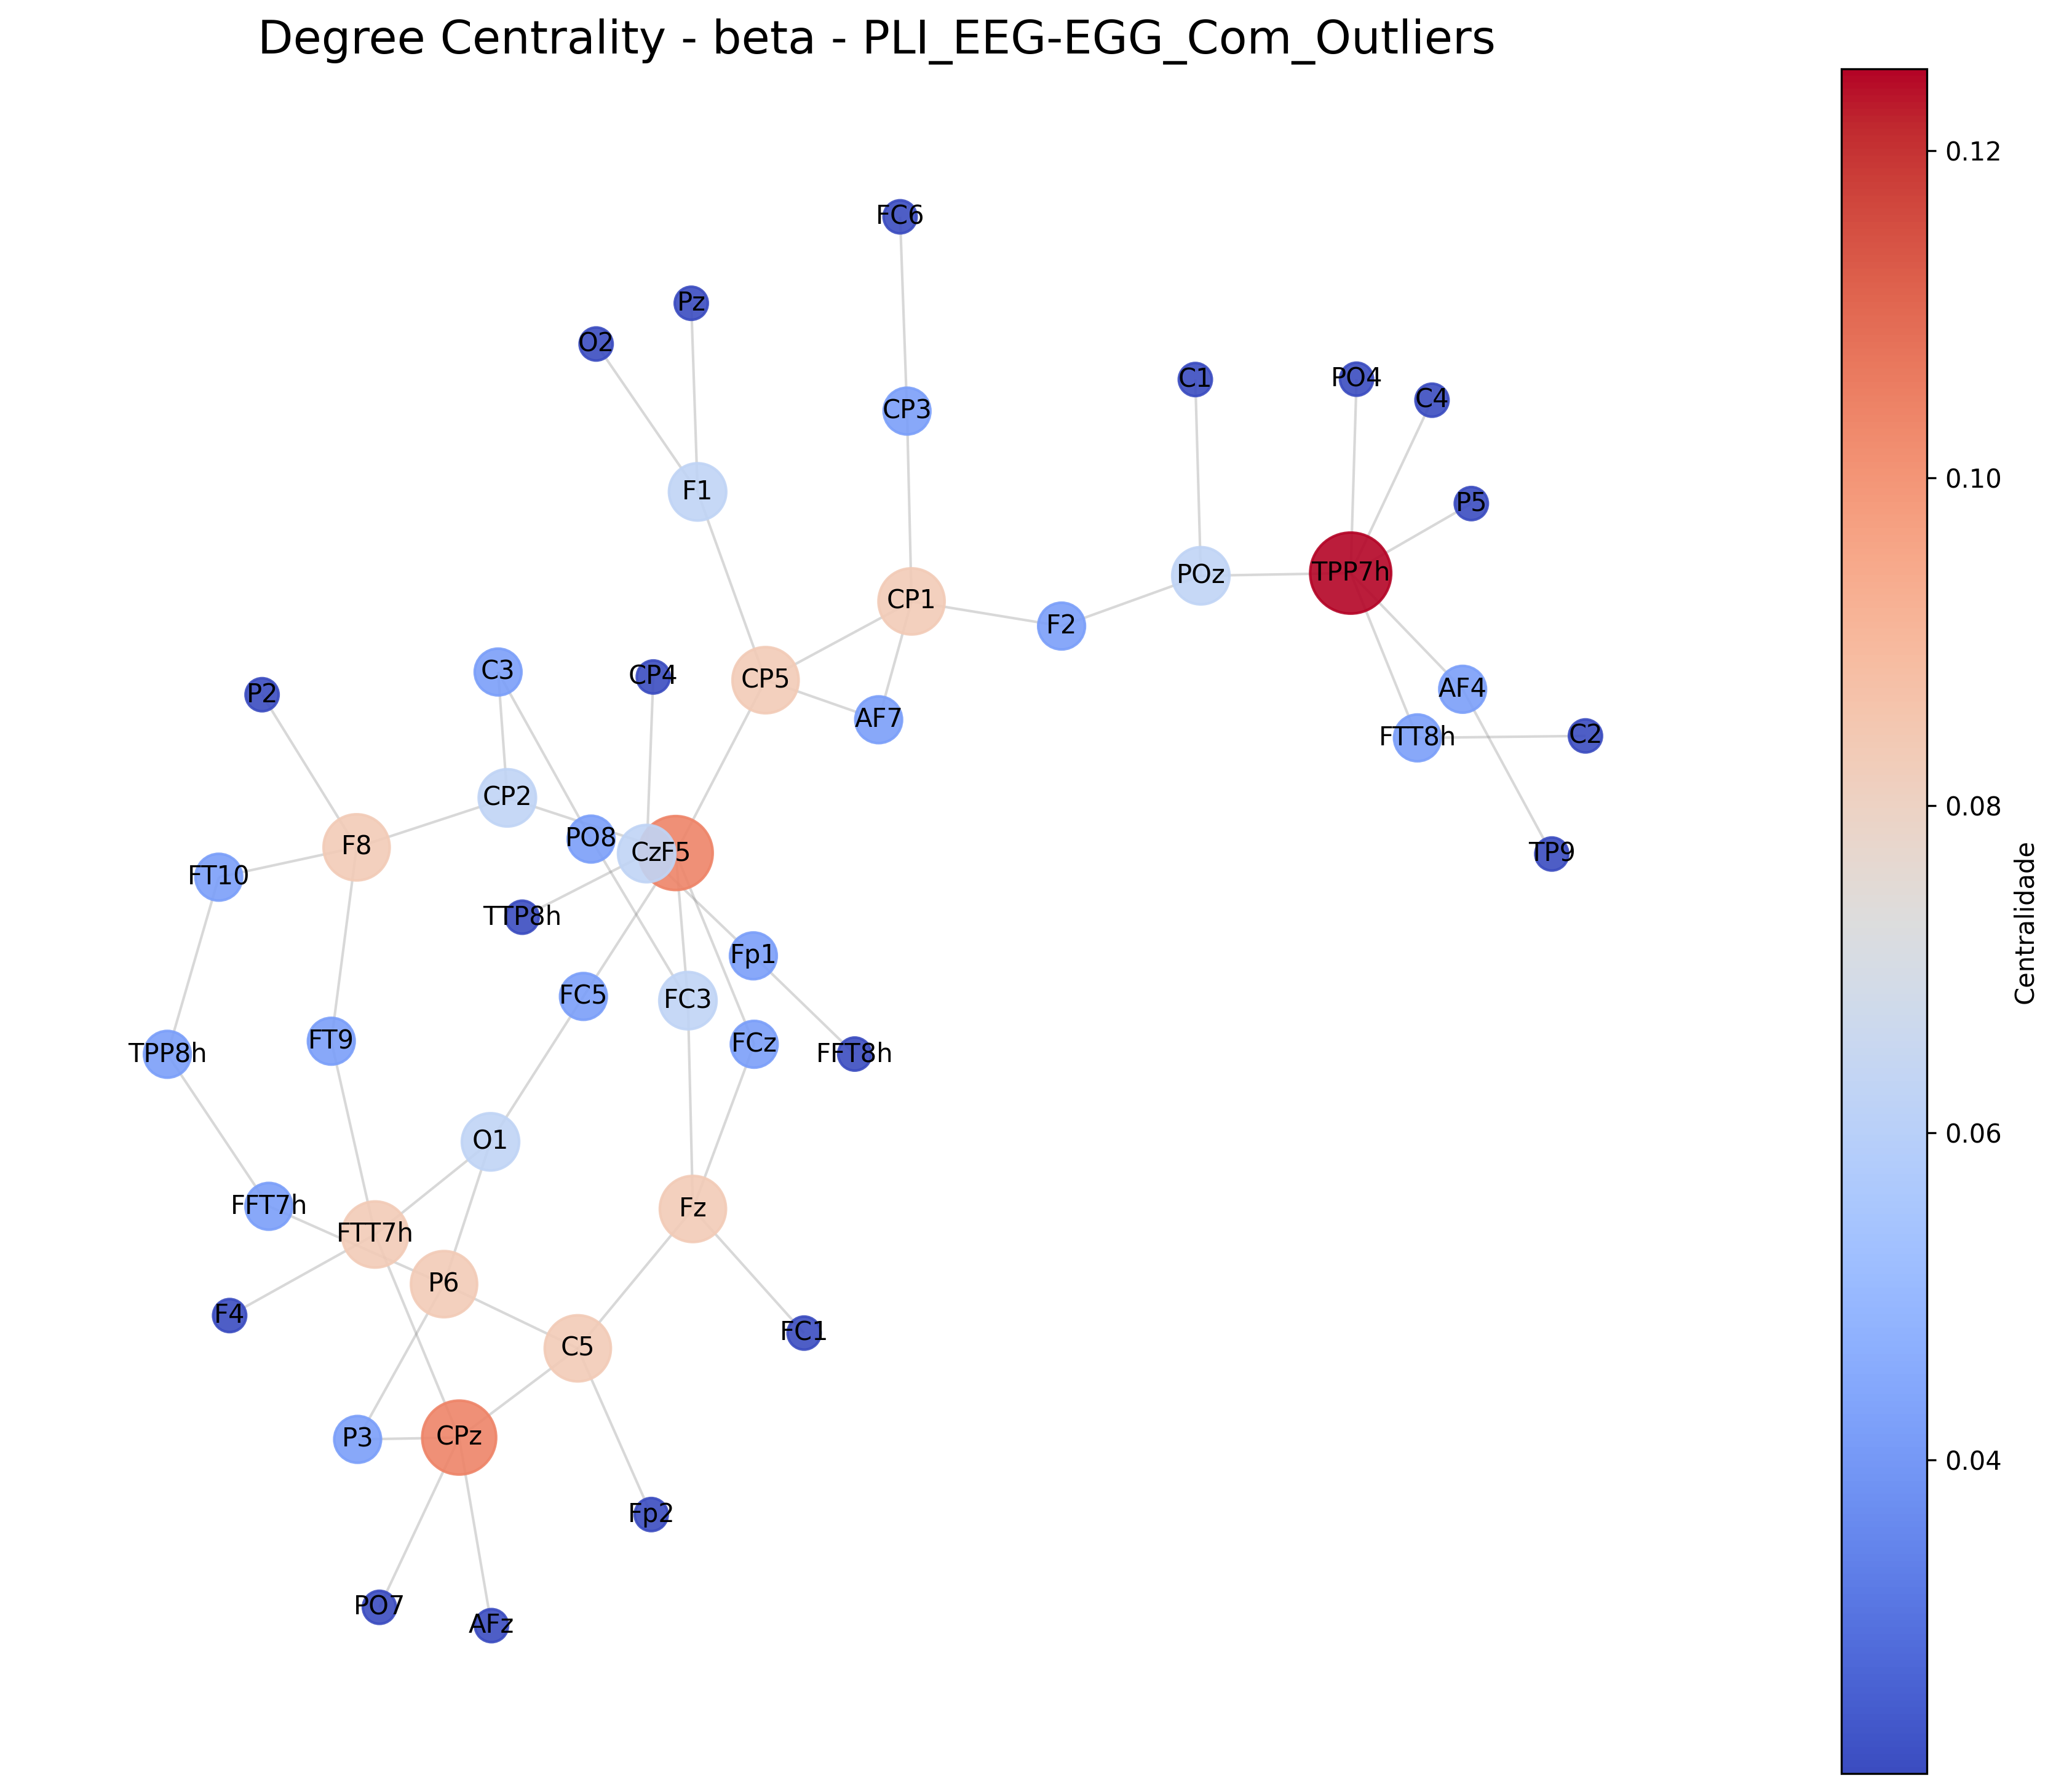
\includegraphics[width=0.45\textwidth]{figs/7_bootstrap_results_analysis/3_centrality_graphs/Com_Outliers/Degree_Centrality__beta__PLI_EEGEGG_Com_Outliers.png}
    }
    \hfill
    \subfloat[\small \textbf{Sem Outliers:} Hierarquia – 1. \textbf{TPP7h}; 2. \textbf{FTT7h, CPz}; 3. \textbf{CP5, F5, CP2, FTT7h}.]{%
        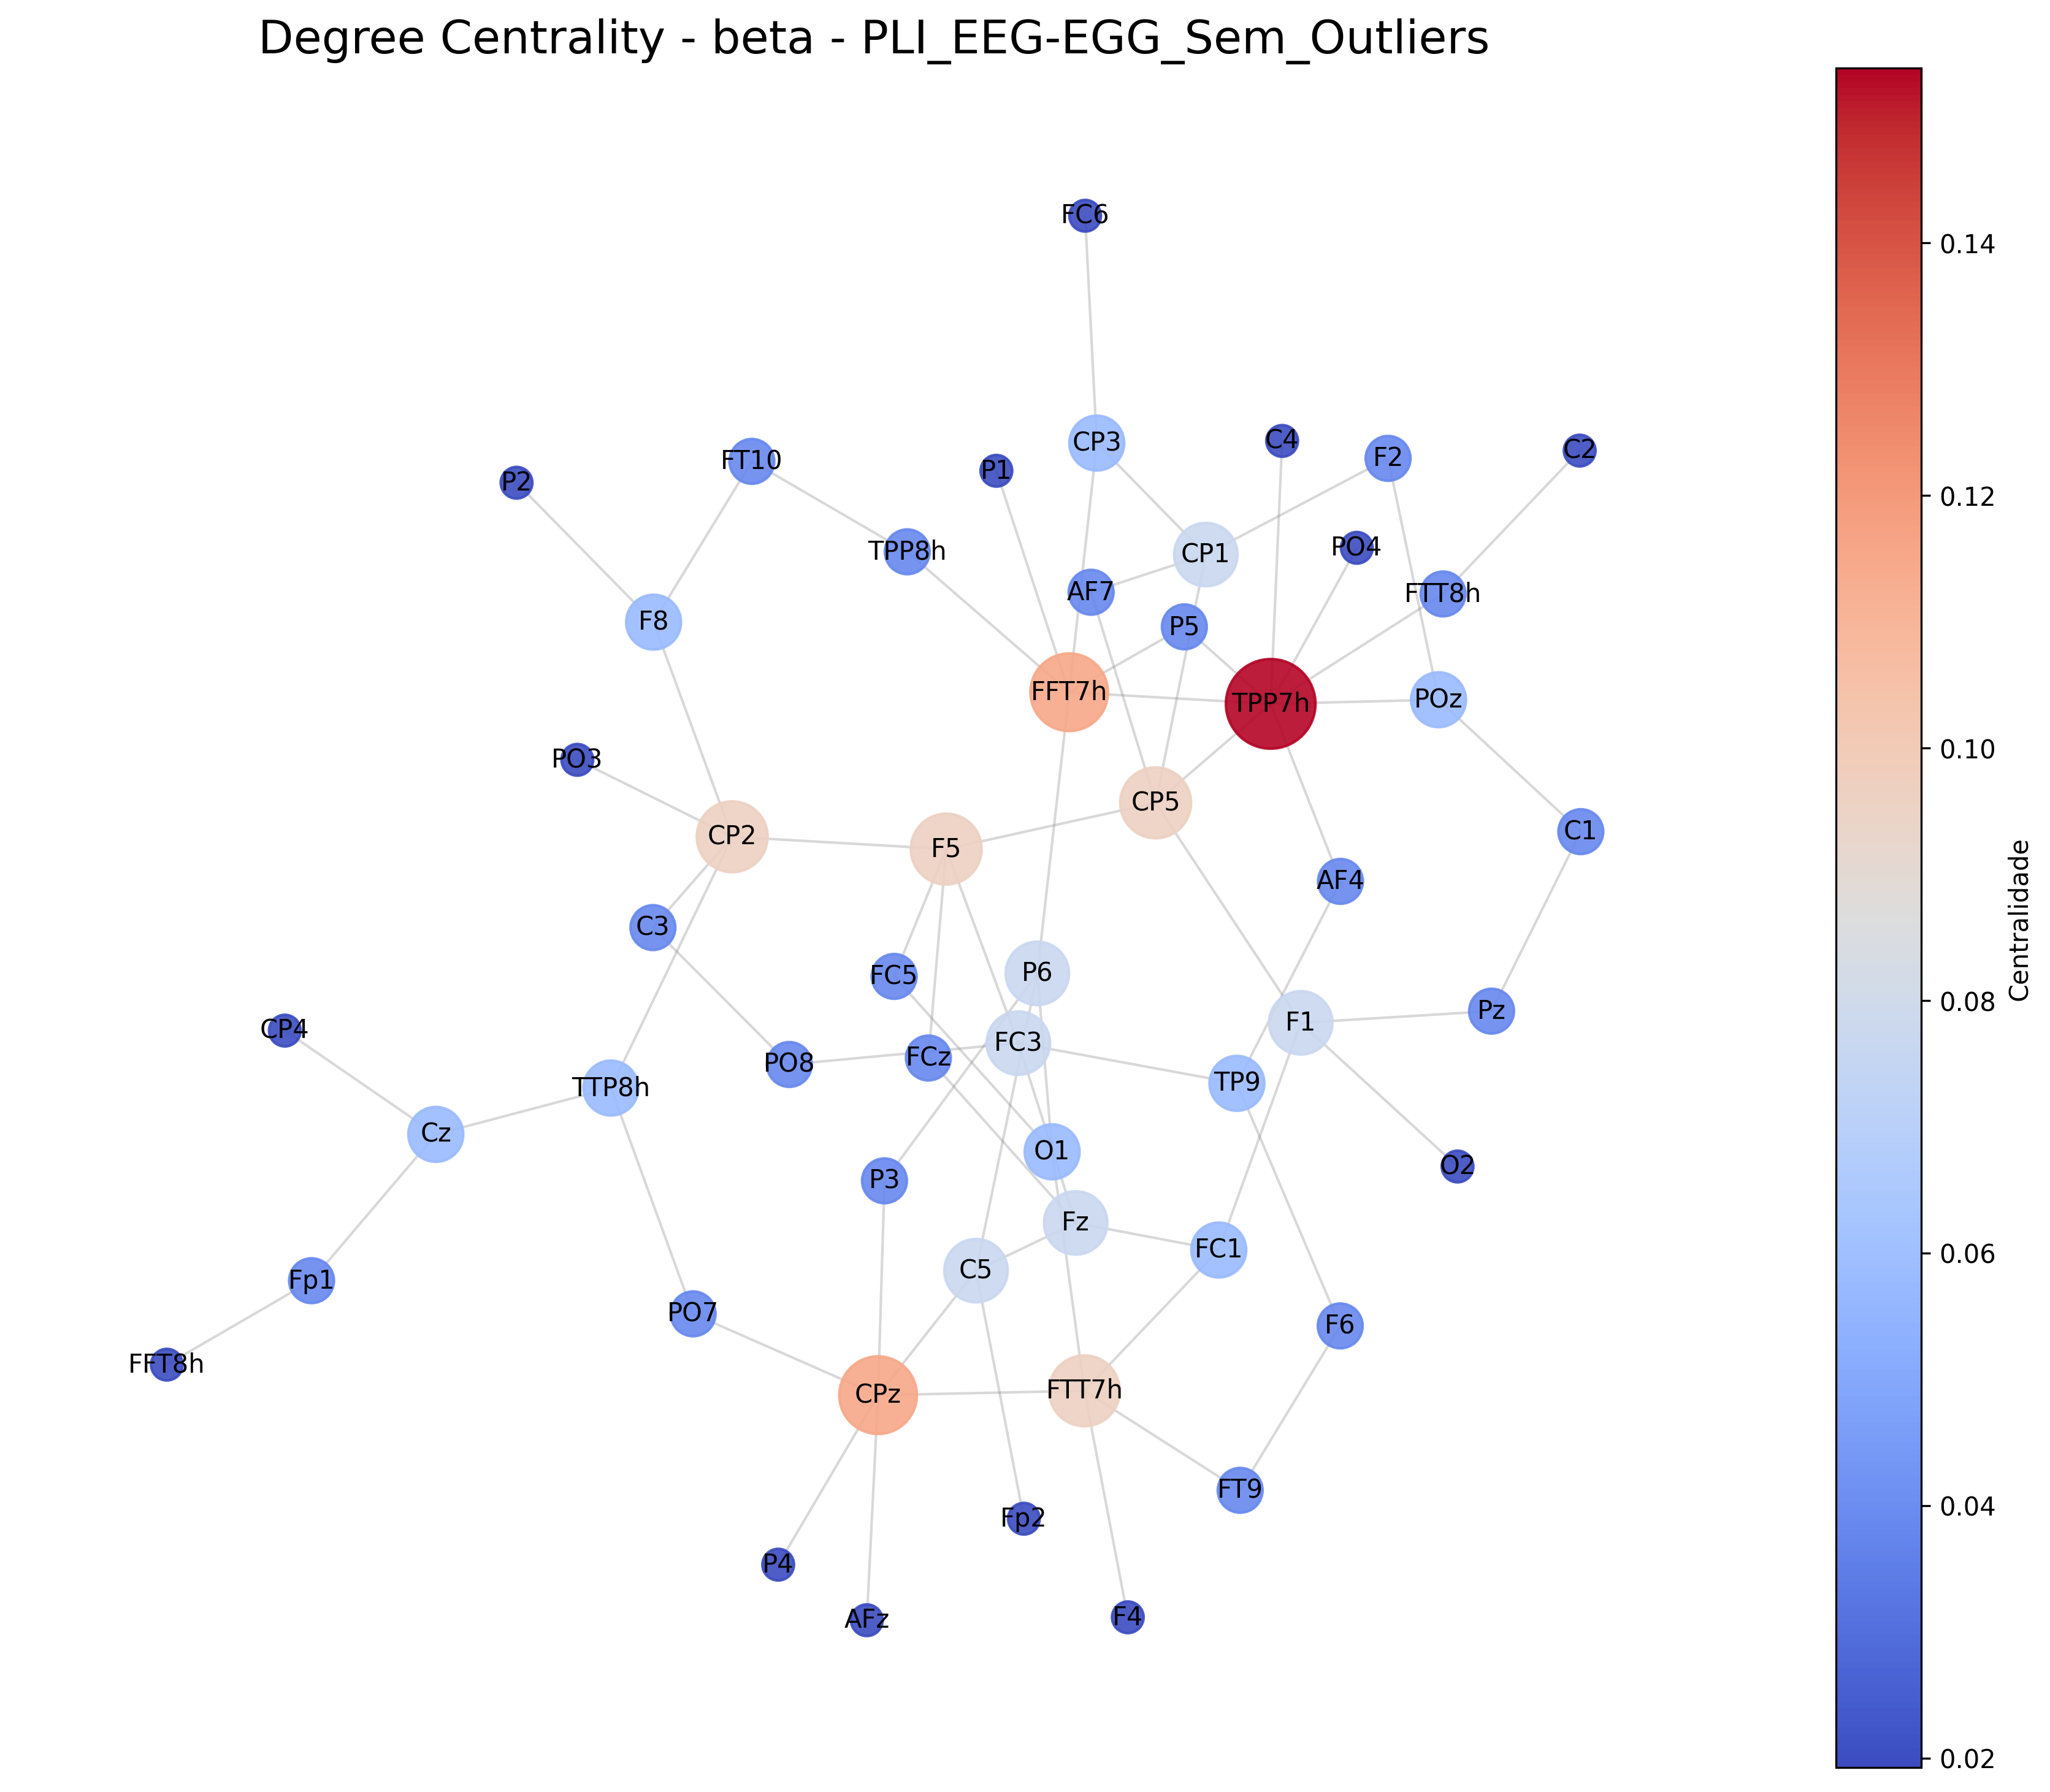
\includegraphics[width=0.45\textwidth]{figs/7_bootstrap_results_analysis/3_centrality_graphs/Sem_Outliers/Degree_Centrality__beta__PLI_EEGEGG_Sem_Outliers.png}
    }
    \caption{\small \textbf{Degree Centrality – Banda Beta (13--30 Hz):} A hierarquia na rede beta destaca consistentemente \textbf{TPP7h} como o hub principal, com pequenas variações na ordem dos outros canais entre os cenários.}
    \label{fig:degree_beta}
\end{figure}

\subsubsection{Eigenvector Centrality}
\begin{figure}[H]
    \centering
    \subfloat[\small \textbf{Com Outliers:} Hierarquia – 1. \textbf{F5}; 2. \textbf{C5, CPz}; 3. \textbf{P6, Fz}; 4. \textbf{CP5, O1, FFT7h, FC3}.]{%
        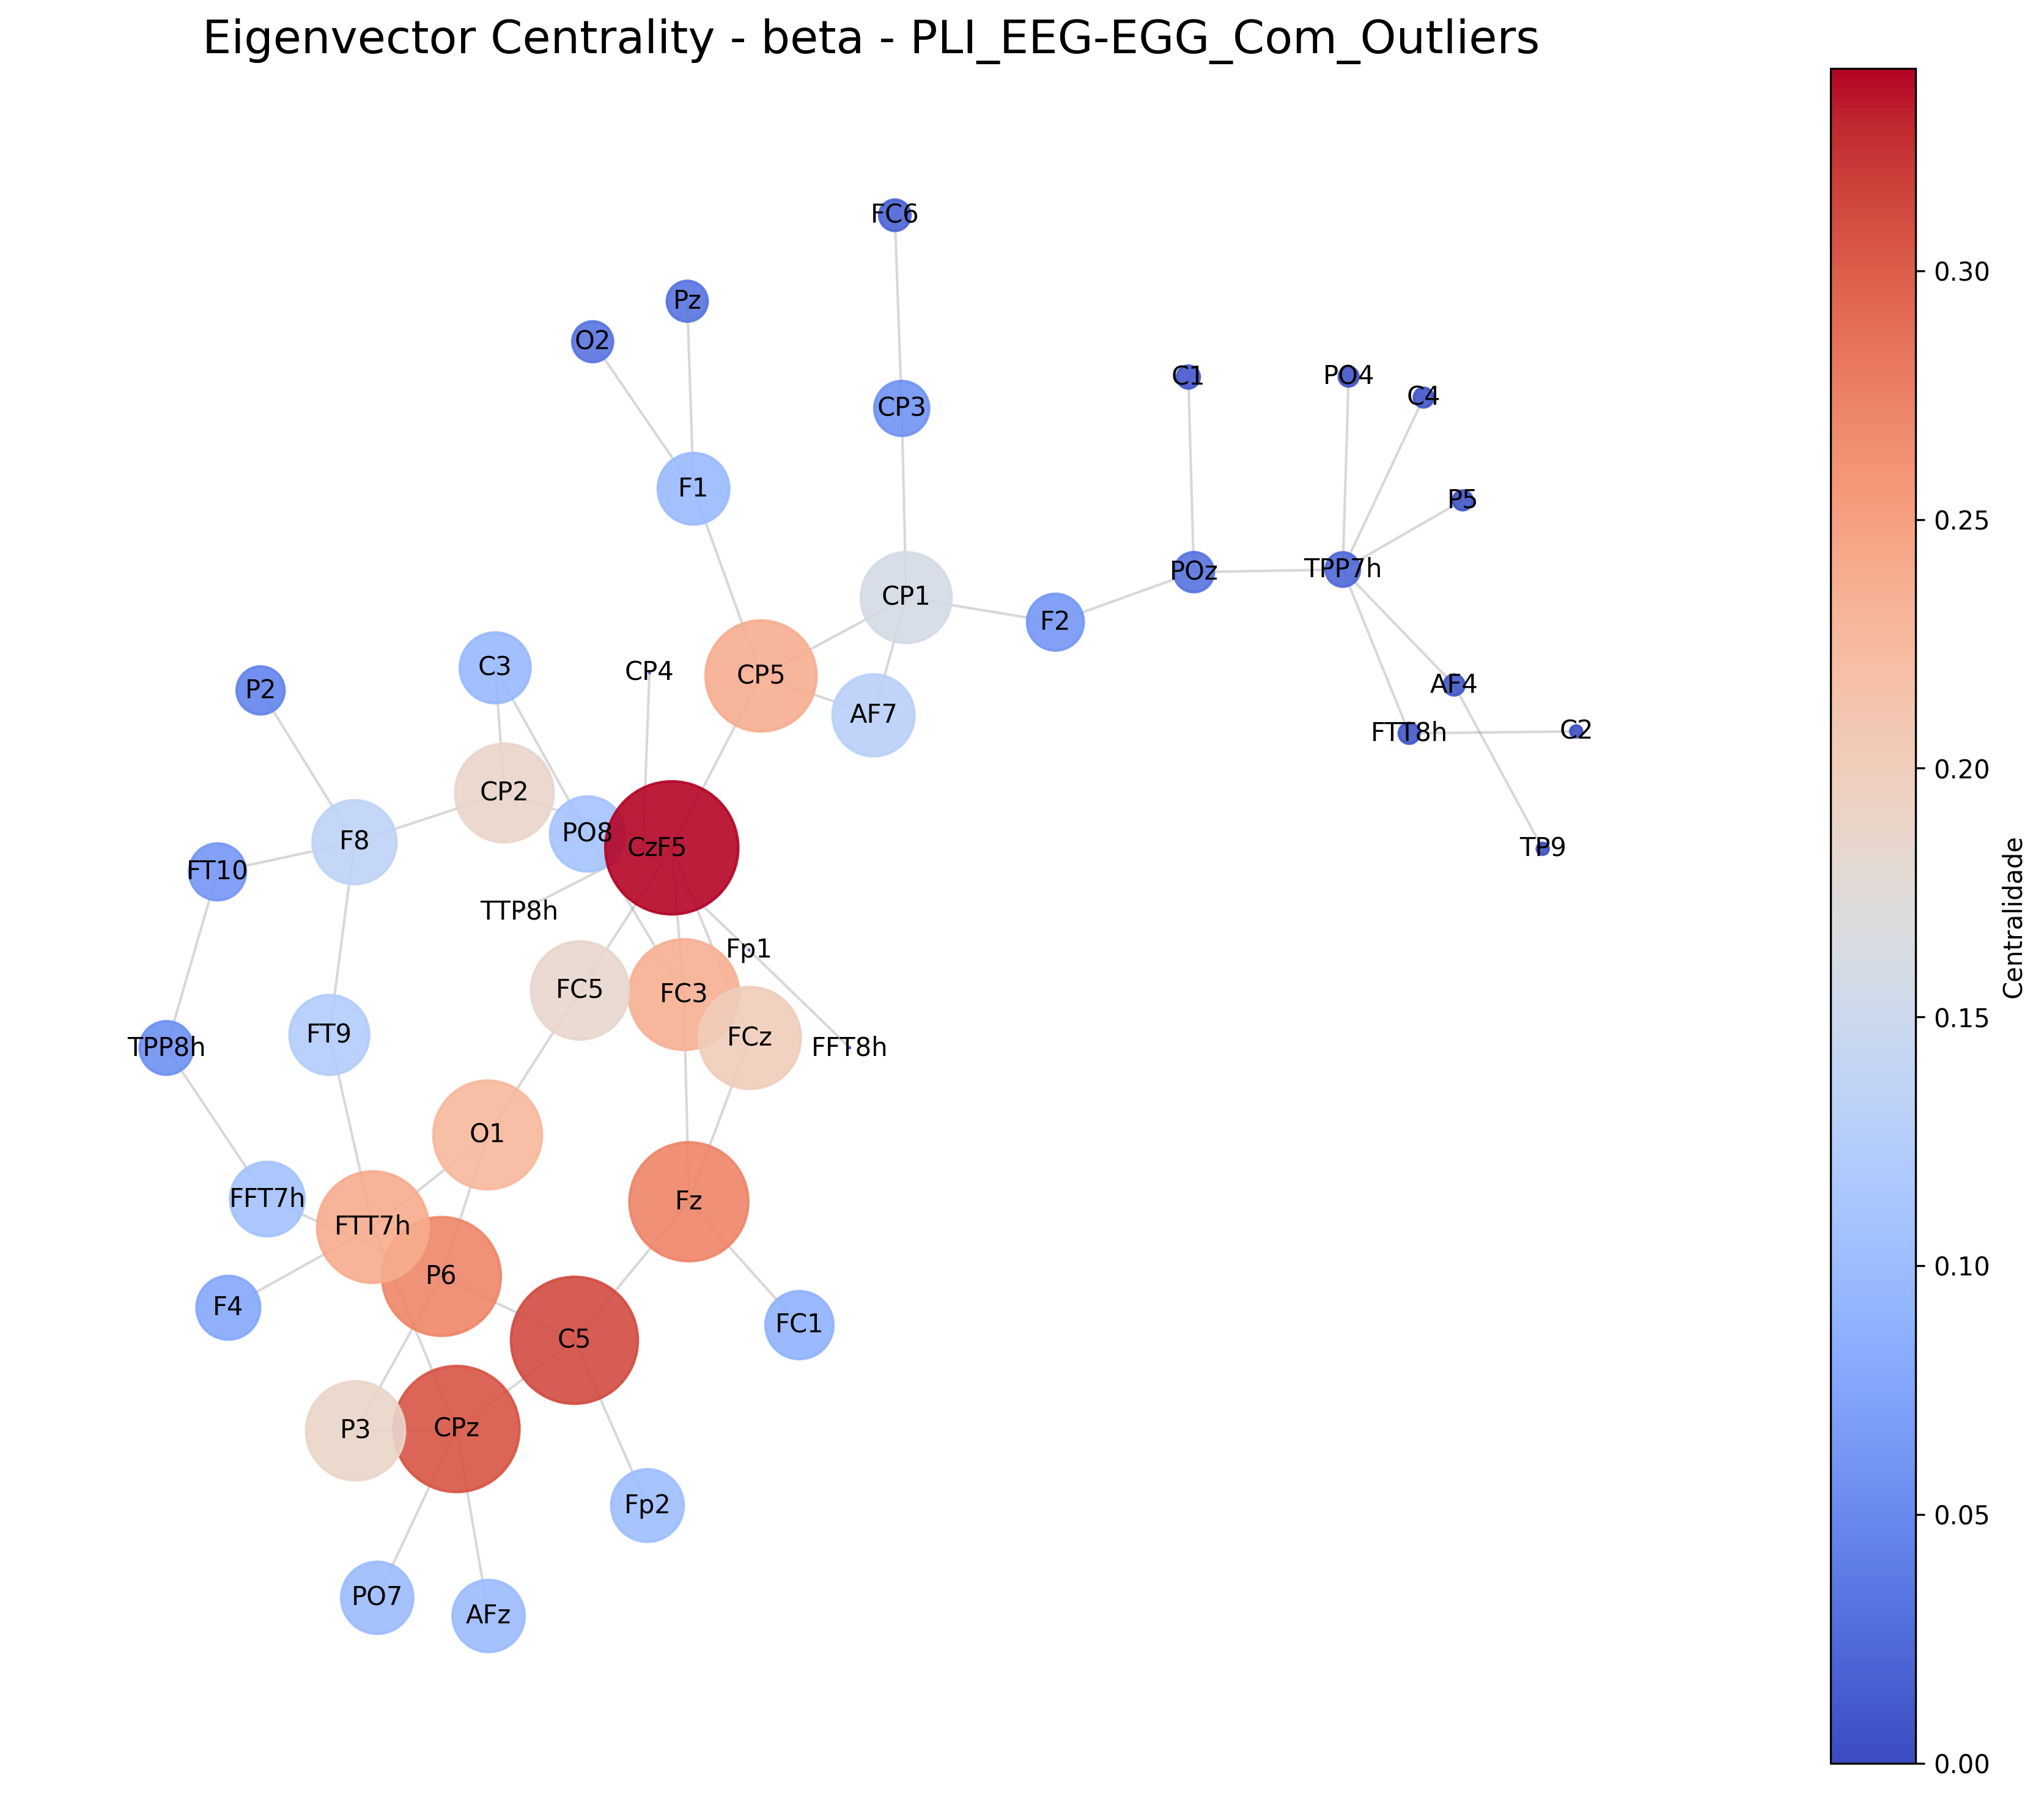
\includegraphics[width=0.45\textwidth]{figs/7_bootstrap_results_analysis/3_centrality_graphs/Com_Outliers/Eigenvector_Centrality__beta__PLI_EEGEGG_Com_Outliers.png}
    }
    \hfill
    \subfloat[\small \textbf{Sem Outliers:} Hierarquia – 1. \textbf{TPP7h}; 2. \textbf{FTT7h}; 3. \textbf{CP5}.]{%
        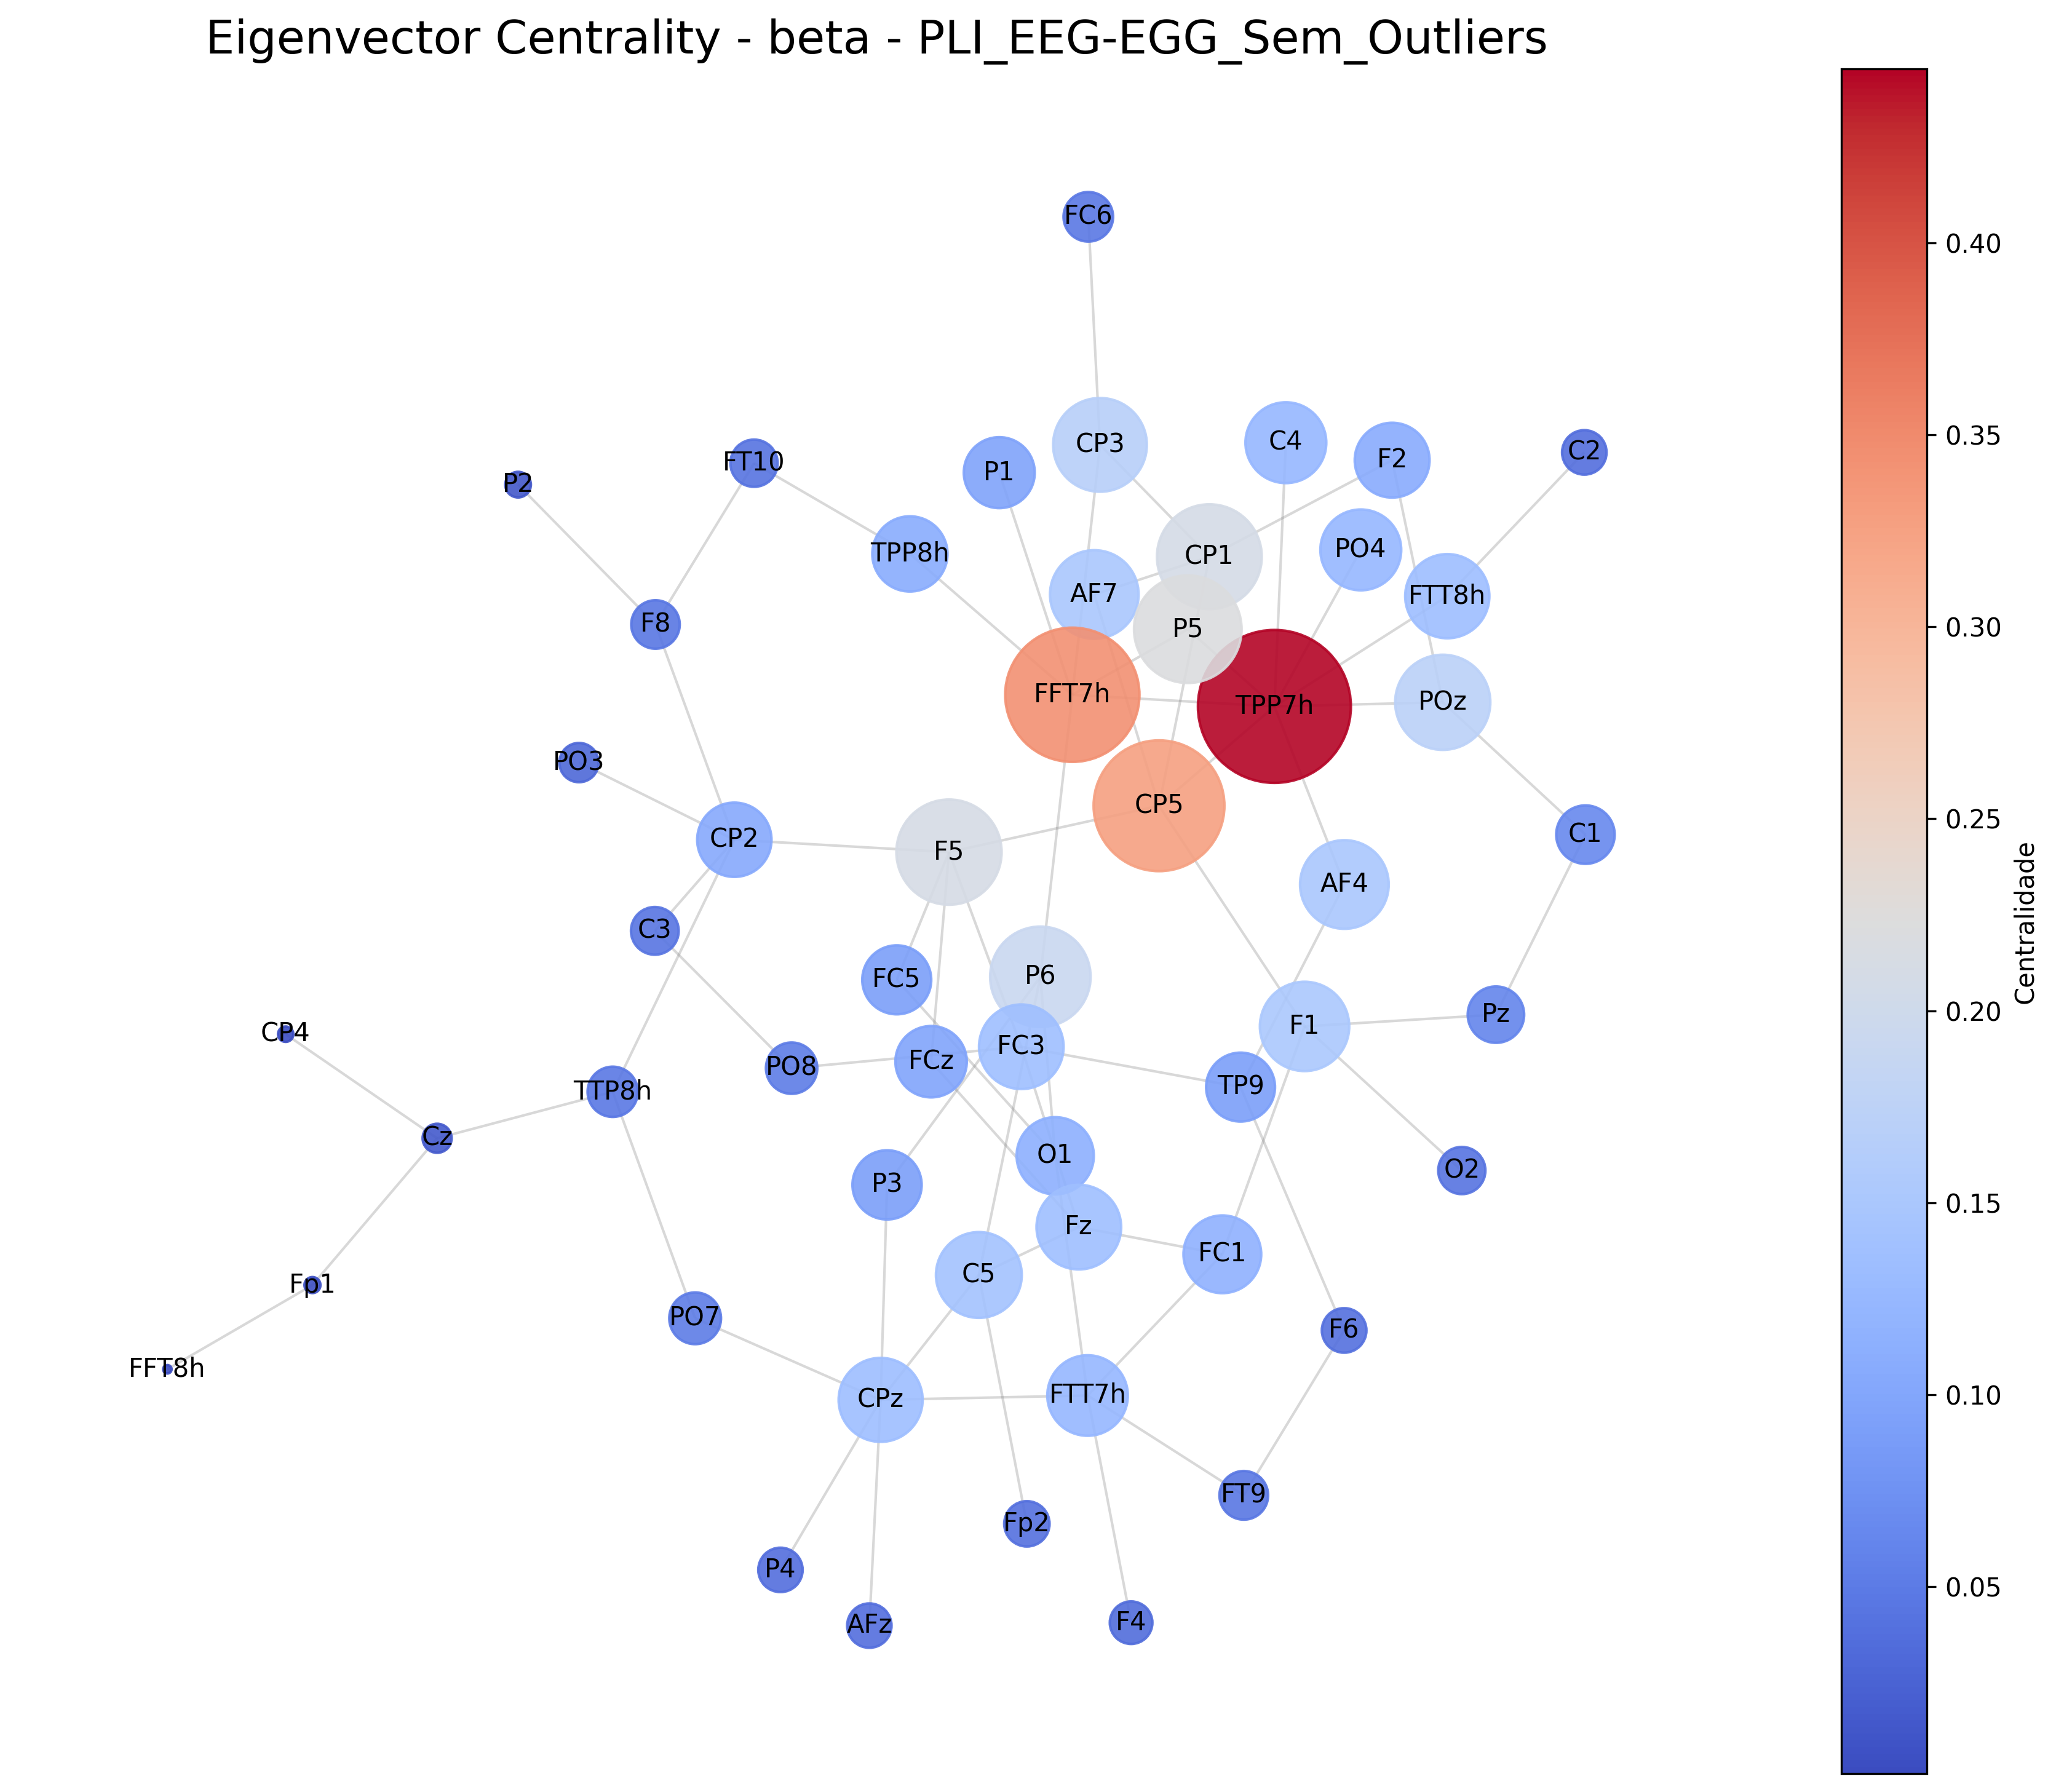
\includegraphics[width=0.45\textwidth]{figs/7_bootstrap_results_analysis/3_centrality_graphs/Sem_Outliers/Eigenvector_Centrality__beta__PLI_EEGEGG_Sem_Outliers.png}
    }
    \caption{\small \textbf{Eigenvector Centrality – Banda Beta (13--30 Hz):} A influência dos canais na rede beta muda de forma notável entre os cenários, com \textbf{TPP7h} emergindo como nodo de maior influência na versão sem outliers.}
    \label{fig:eigenvector_beta}
\end{figure}

\subsection{Banda Delta (0.5--4 Hz)}
\subsubsection{Betweenness Centrality}
\begin{figure}[H]
    \centering
    \subfloat[\small \textbf{Com Outliers:} Hierarquia – Único nodo destacado: \textbf{Fp2}.]{%
        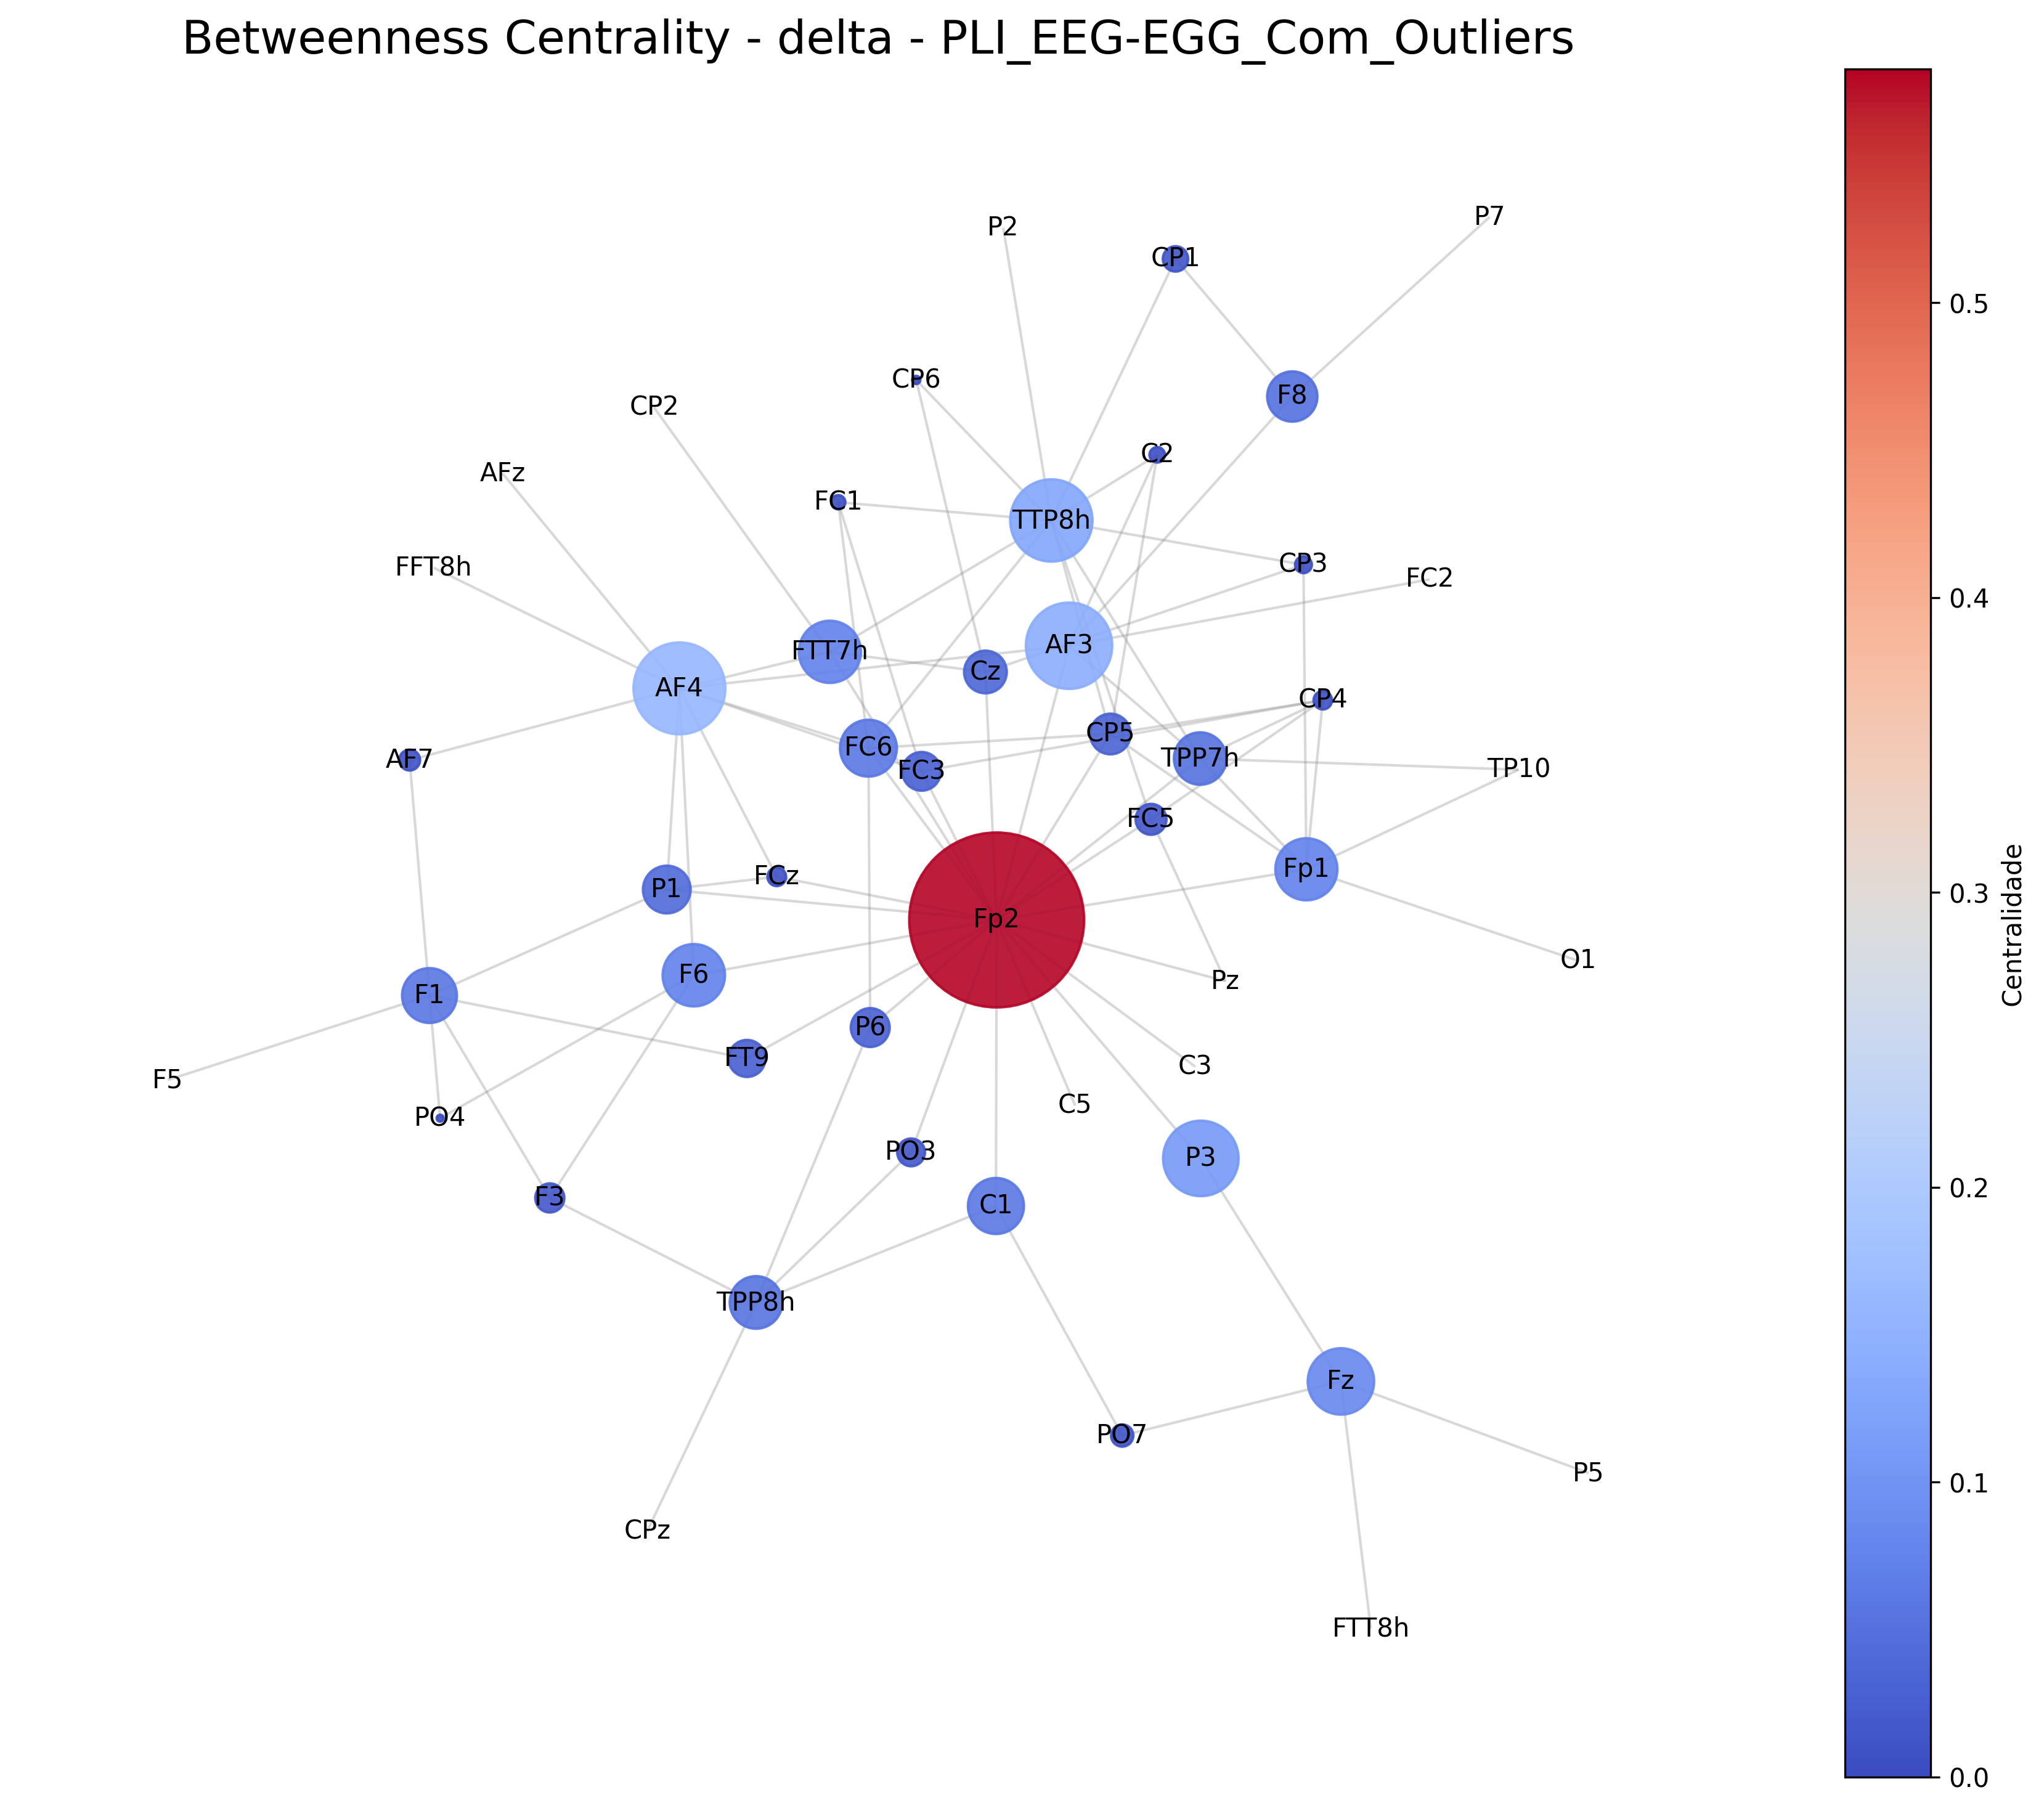
\includegraphics[width=0.45\textwidth]{figs/7_bootstrap_results_analysis/3_centrality_graphs/Com_Outliers/Betweenness_Centrality__delta__PLI_EEGEGG_Com_Outliers.png}
    }
    \hfill
    \subfloat[\small \textbf{Sem Outliers:} Hierarquia – 1. \textbf{CP5, CP4}; 2. \textbf{FC3}; 3. \textbf{AF4}; 4. \textbf{FFT8h}.]{%
        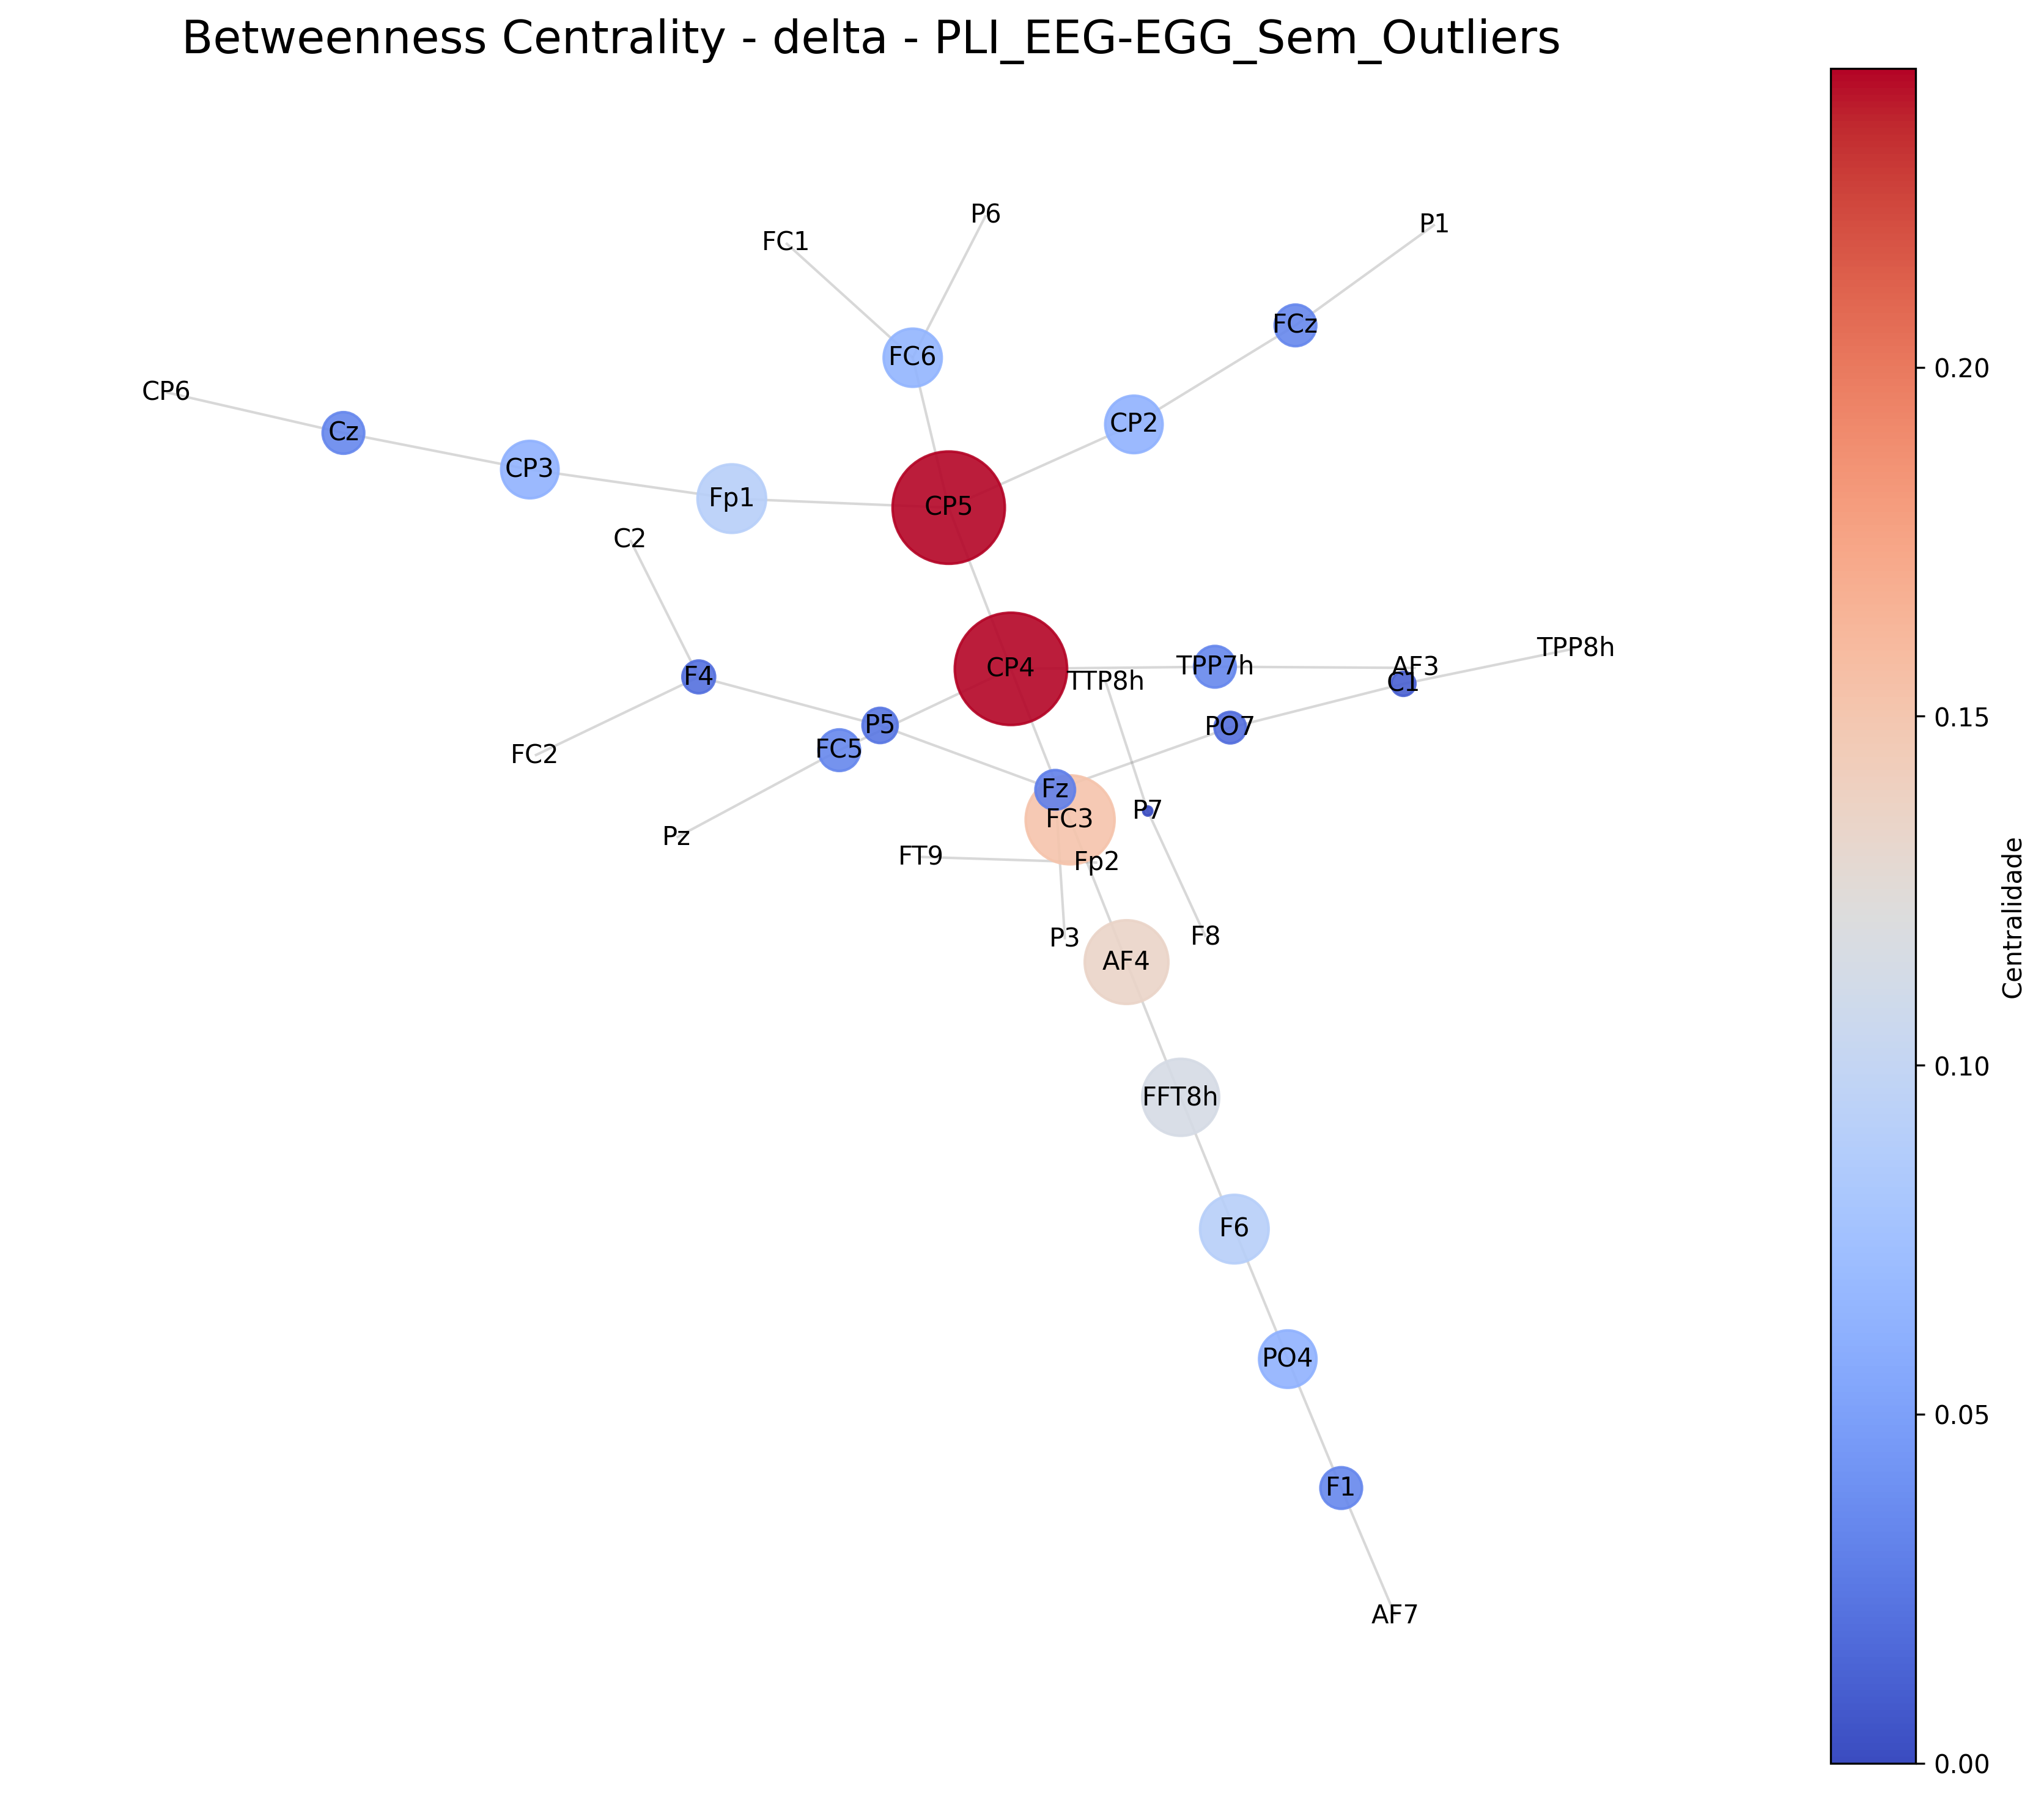
\includegraphics[width=0.45\textwidth]{figs/7_bootstrap_results_analysis/3_centrality_graphs/Sem_Outliers/Betweenness_Centrality__delta__PLI_EEGEGG_Sem_Outliers.png}
    }
    \caption{\small \textbf{Betweenness Centrality – Banda Delta (0.5--4 Hz):} A análise mostra que, com outliers, \textbf{Fp2} se destaca; sem outliers, a centralidade se redistribui com \textbf{CP5} e \textbf{CP4} assumindo papéis principais.}
    \label{fig:betweenness_delta}
\end{figure}

\subsubsection{Degree Centrality}
\begin{figure}[H]
    \centering
    \subfloat[\small \textbf{Com Outliers:} Hierarquia – 1. \textbf{Fp2}; 2. \textbf{TTP8h}; 3. \textbf{AF4}.]{%
        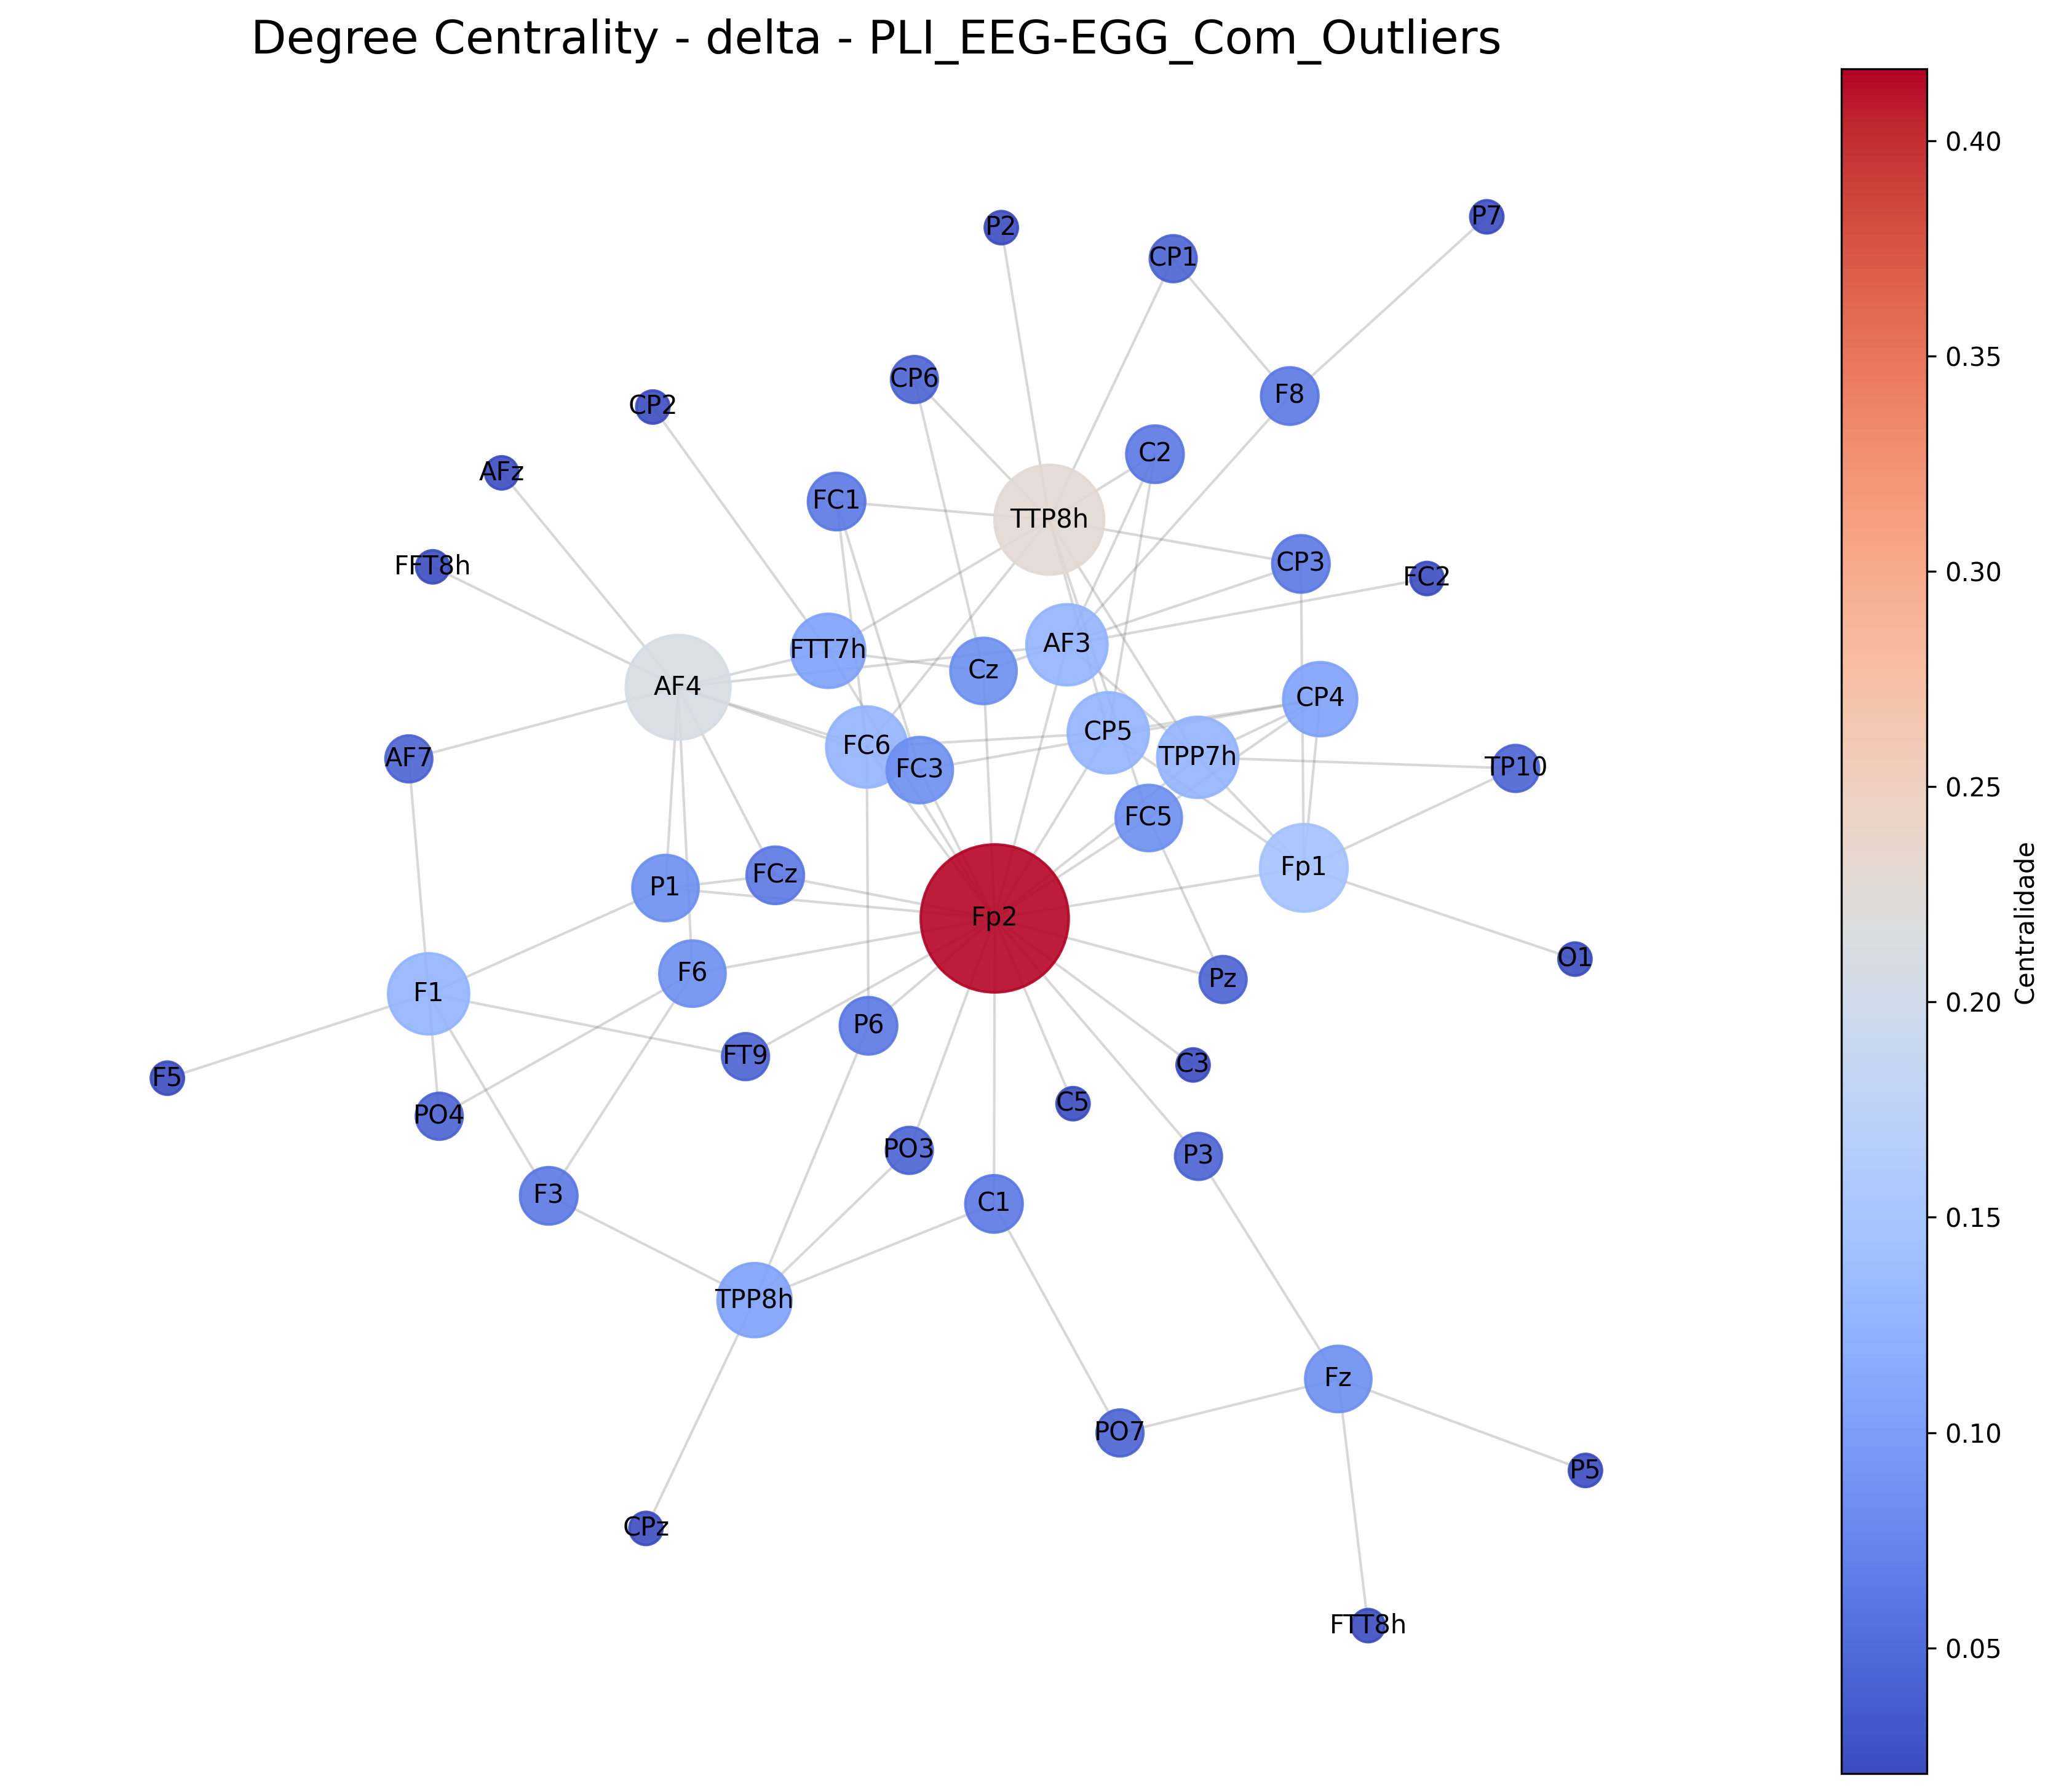
\includegraphics[width=0.45\textwidth]{figs/7_bootstrap_results_analysis/3_centrality_graphs/Com_Outliers/Degree_Centrality__delta__PLI_EEGEGG_Com_Outliers.png}
    }
    \hfill
    \subfloat[\small \textbf{Sem Outliers:} Hierarquia – 1. \textbf{CP5, CP4}; 2. \textbf{FC6, F4, Fz}.]{%
        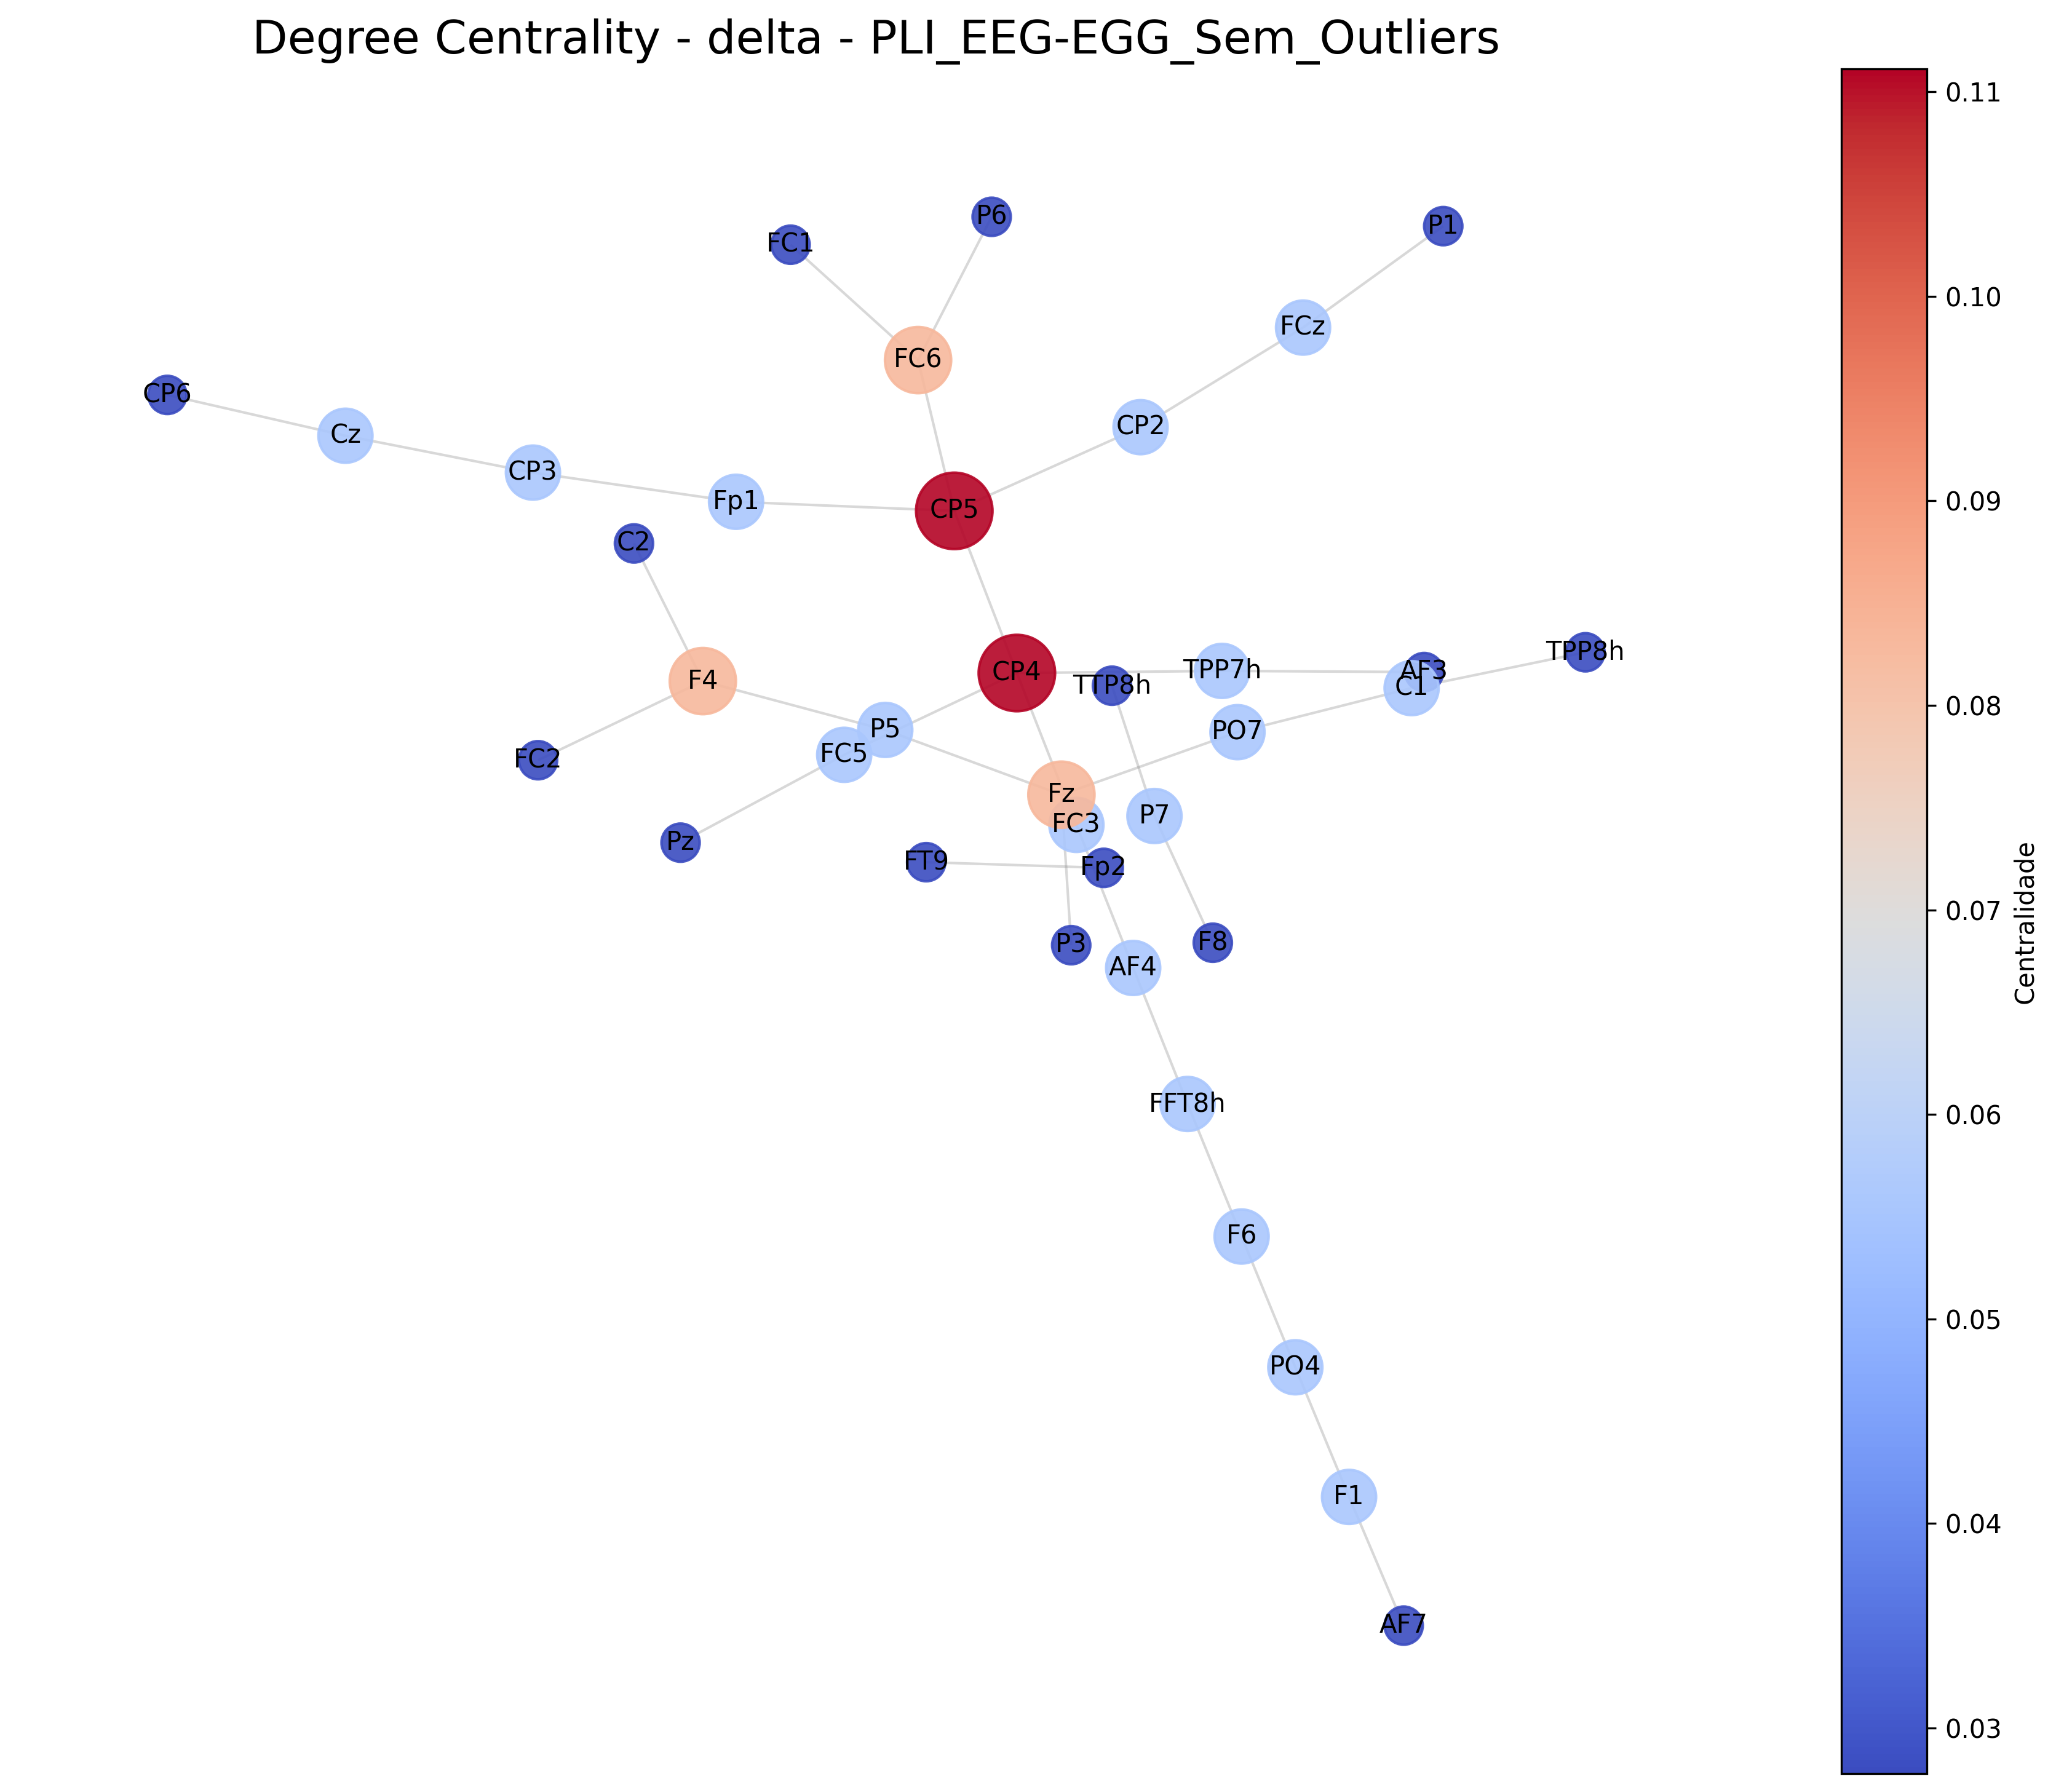
\includegraphics[width=0.45\textwidth]{figs/7_bootstrap_results_analysis/3_centrality_graphs/Sem_Outliers/Degree_Centrality__delta__PLI_EEGEGG_Sem_Outliers.png}
    }
    \caption{\small \textbf{Degree Centrality – Banda Delta (0.5--4 Hz):} A rede delta apresenta uma hierarquia distinta entre os cenários, com \textbf{Fp2} liderando na versão com outliers e um agrupamento parietal (\textbf{CP5, CP4}) emergindo sem outliers.}
    \label{fig:degree_delta}
\end{figure}

\subsubsection{Eigenvector Centrality}
\begin{figure}[H]
    \centering
    \subfloat[\small \textbf{Com Outliers:} Hierarquia – 1. \textbf{Fp2}; 2. \textbf{TTP8h, FC6, CP5, TPP7h}.]{%
        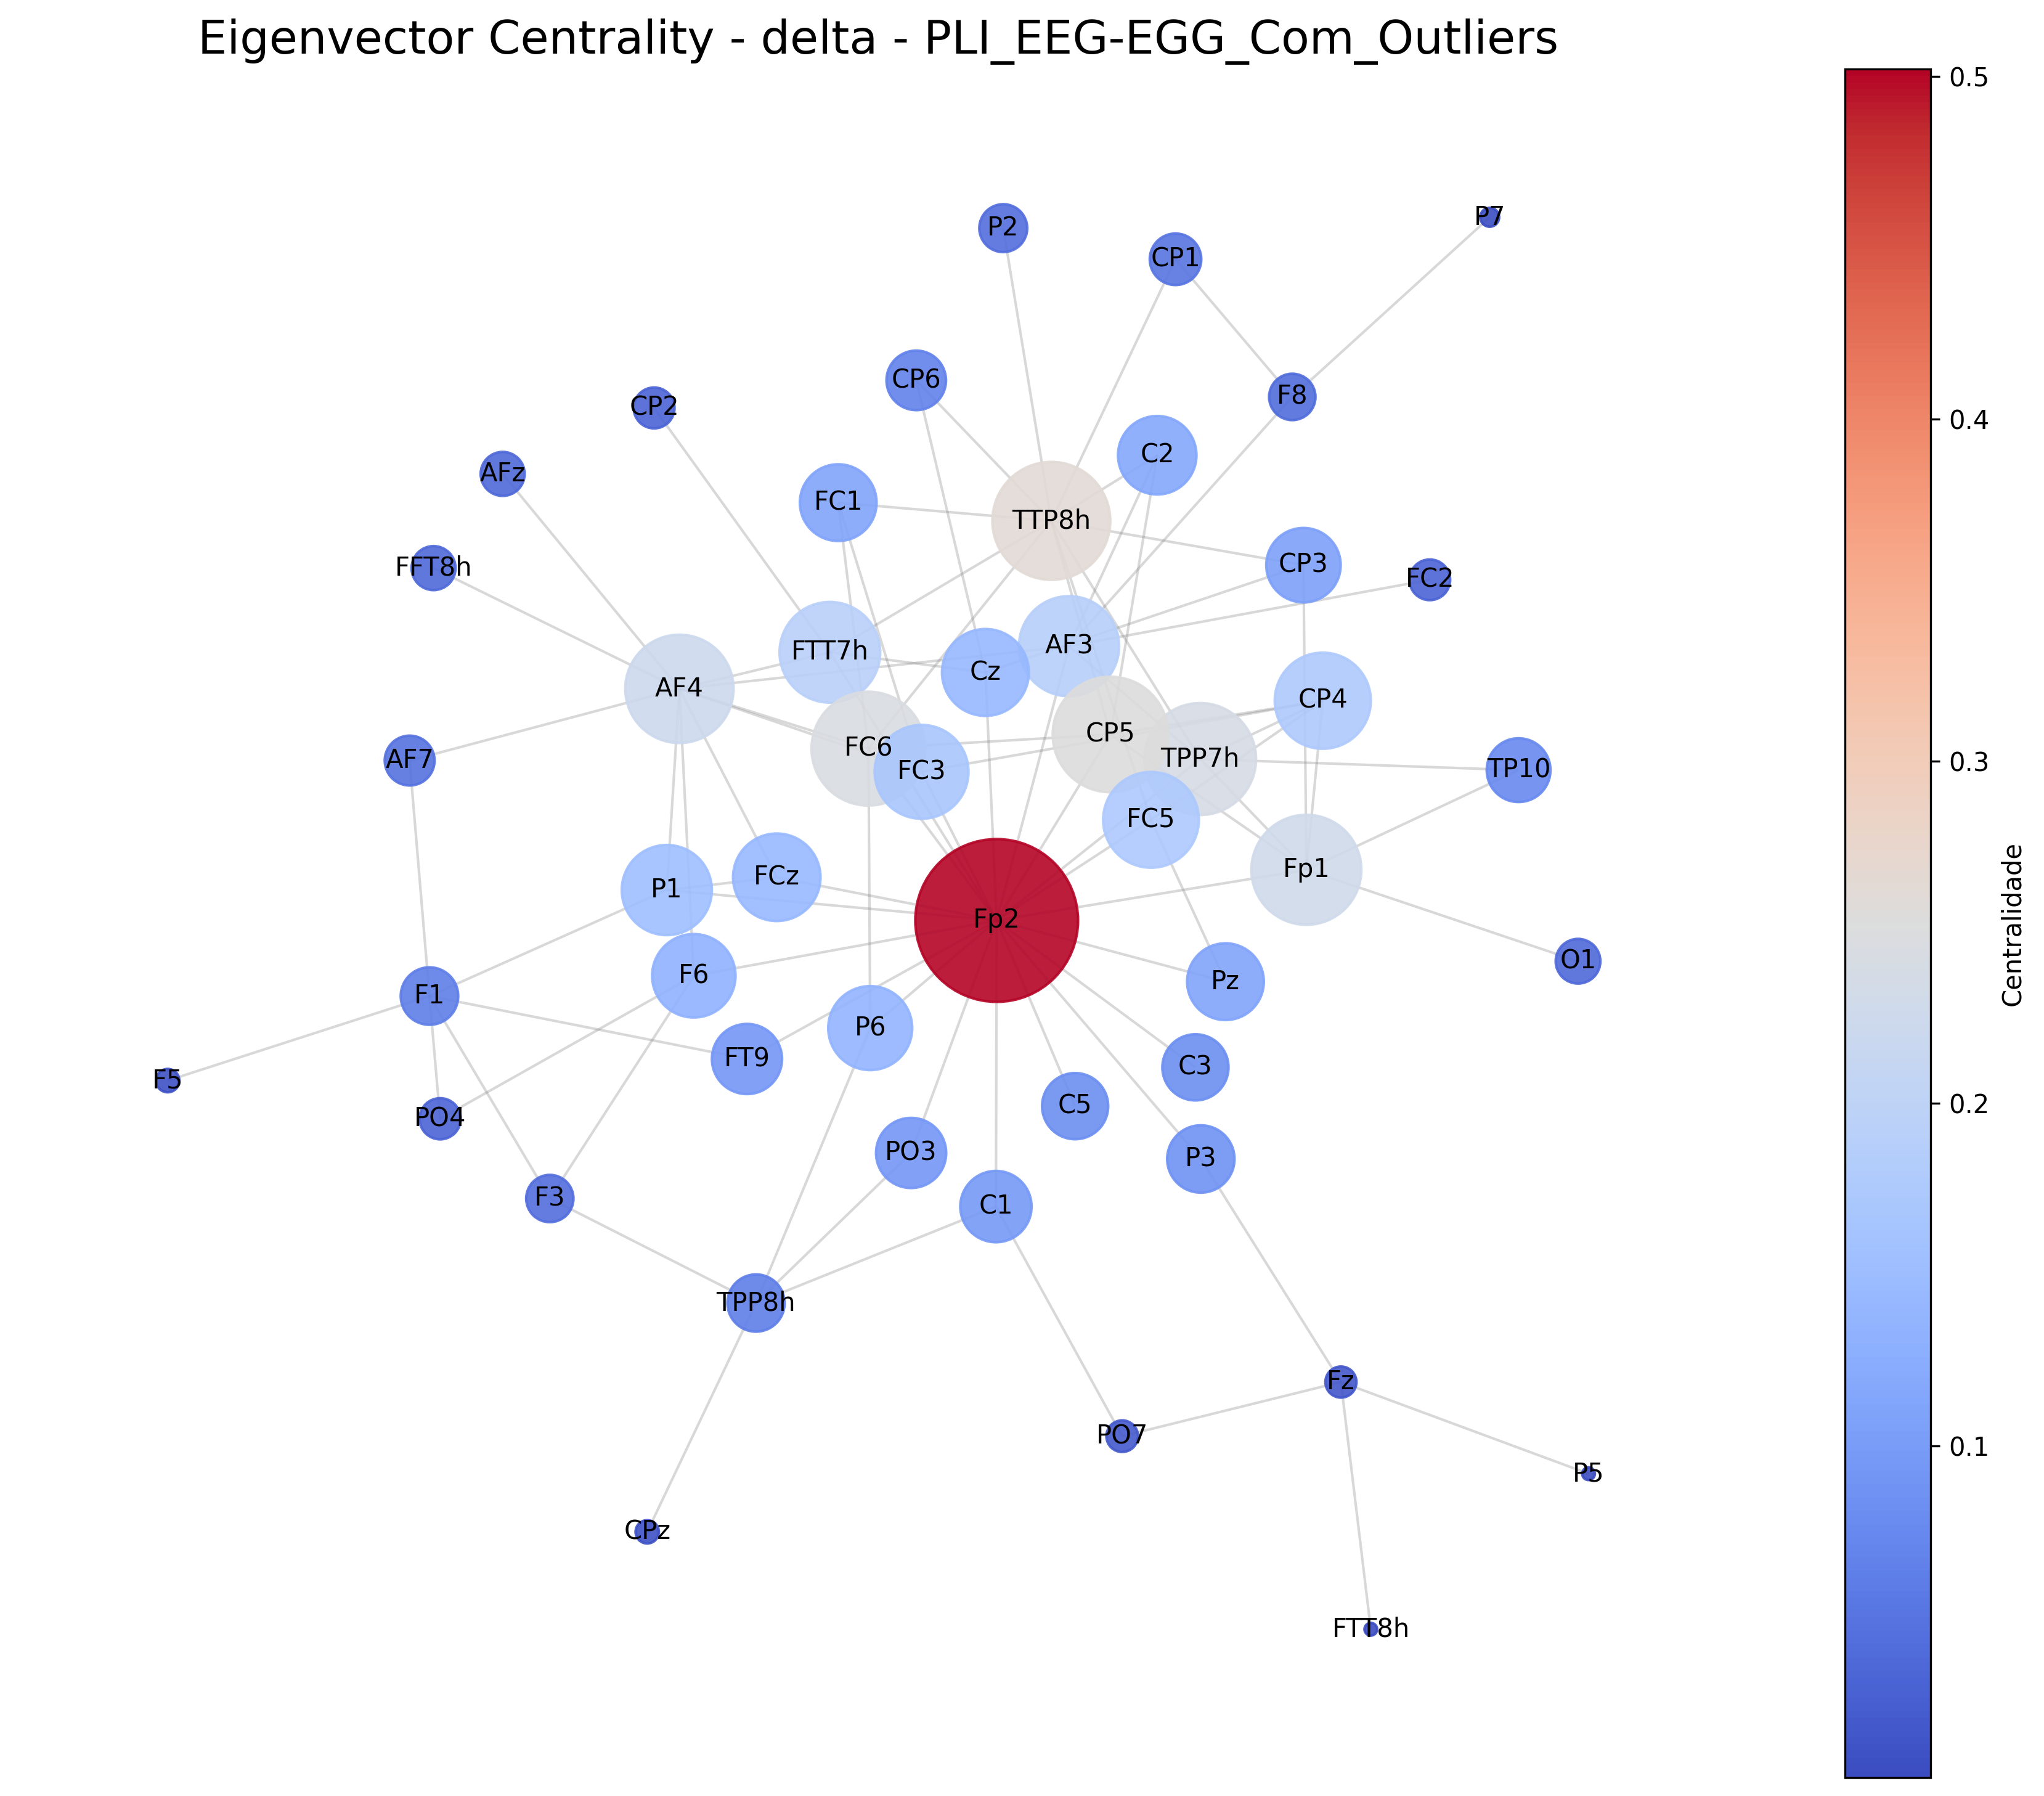
\includegraphics[width=0.45\textwidth]{figs/7_bootstrap_results_analysis/3_centrality_graphs/Com_Outliers/Eigenvector_Centrality__delta__PLI_EEGEGG_Com_Outliers.png}
    }
    \hfill
    \subfloat[\small \textbf{Sem Outliers:} Hierarquia – 1. \textbf{CP5}; 2. \textbf{CP4}; 3. \textbf{FC6}; 4. \textbf{Fp1, CP2, FC3}.]{%
        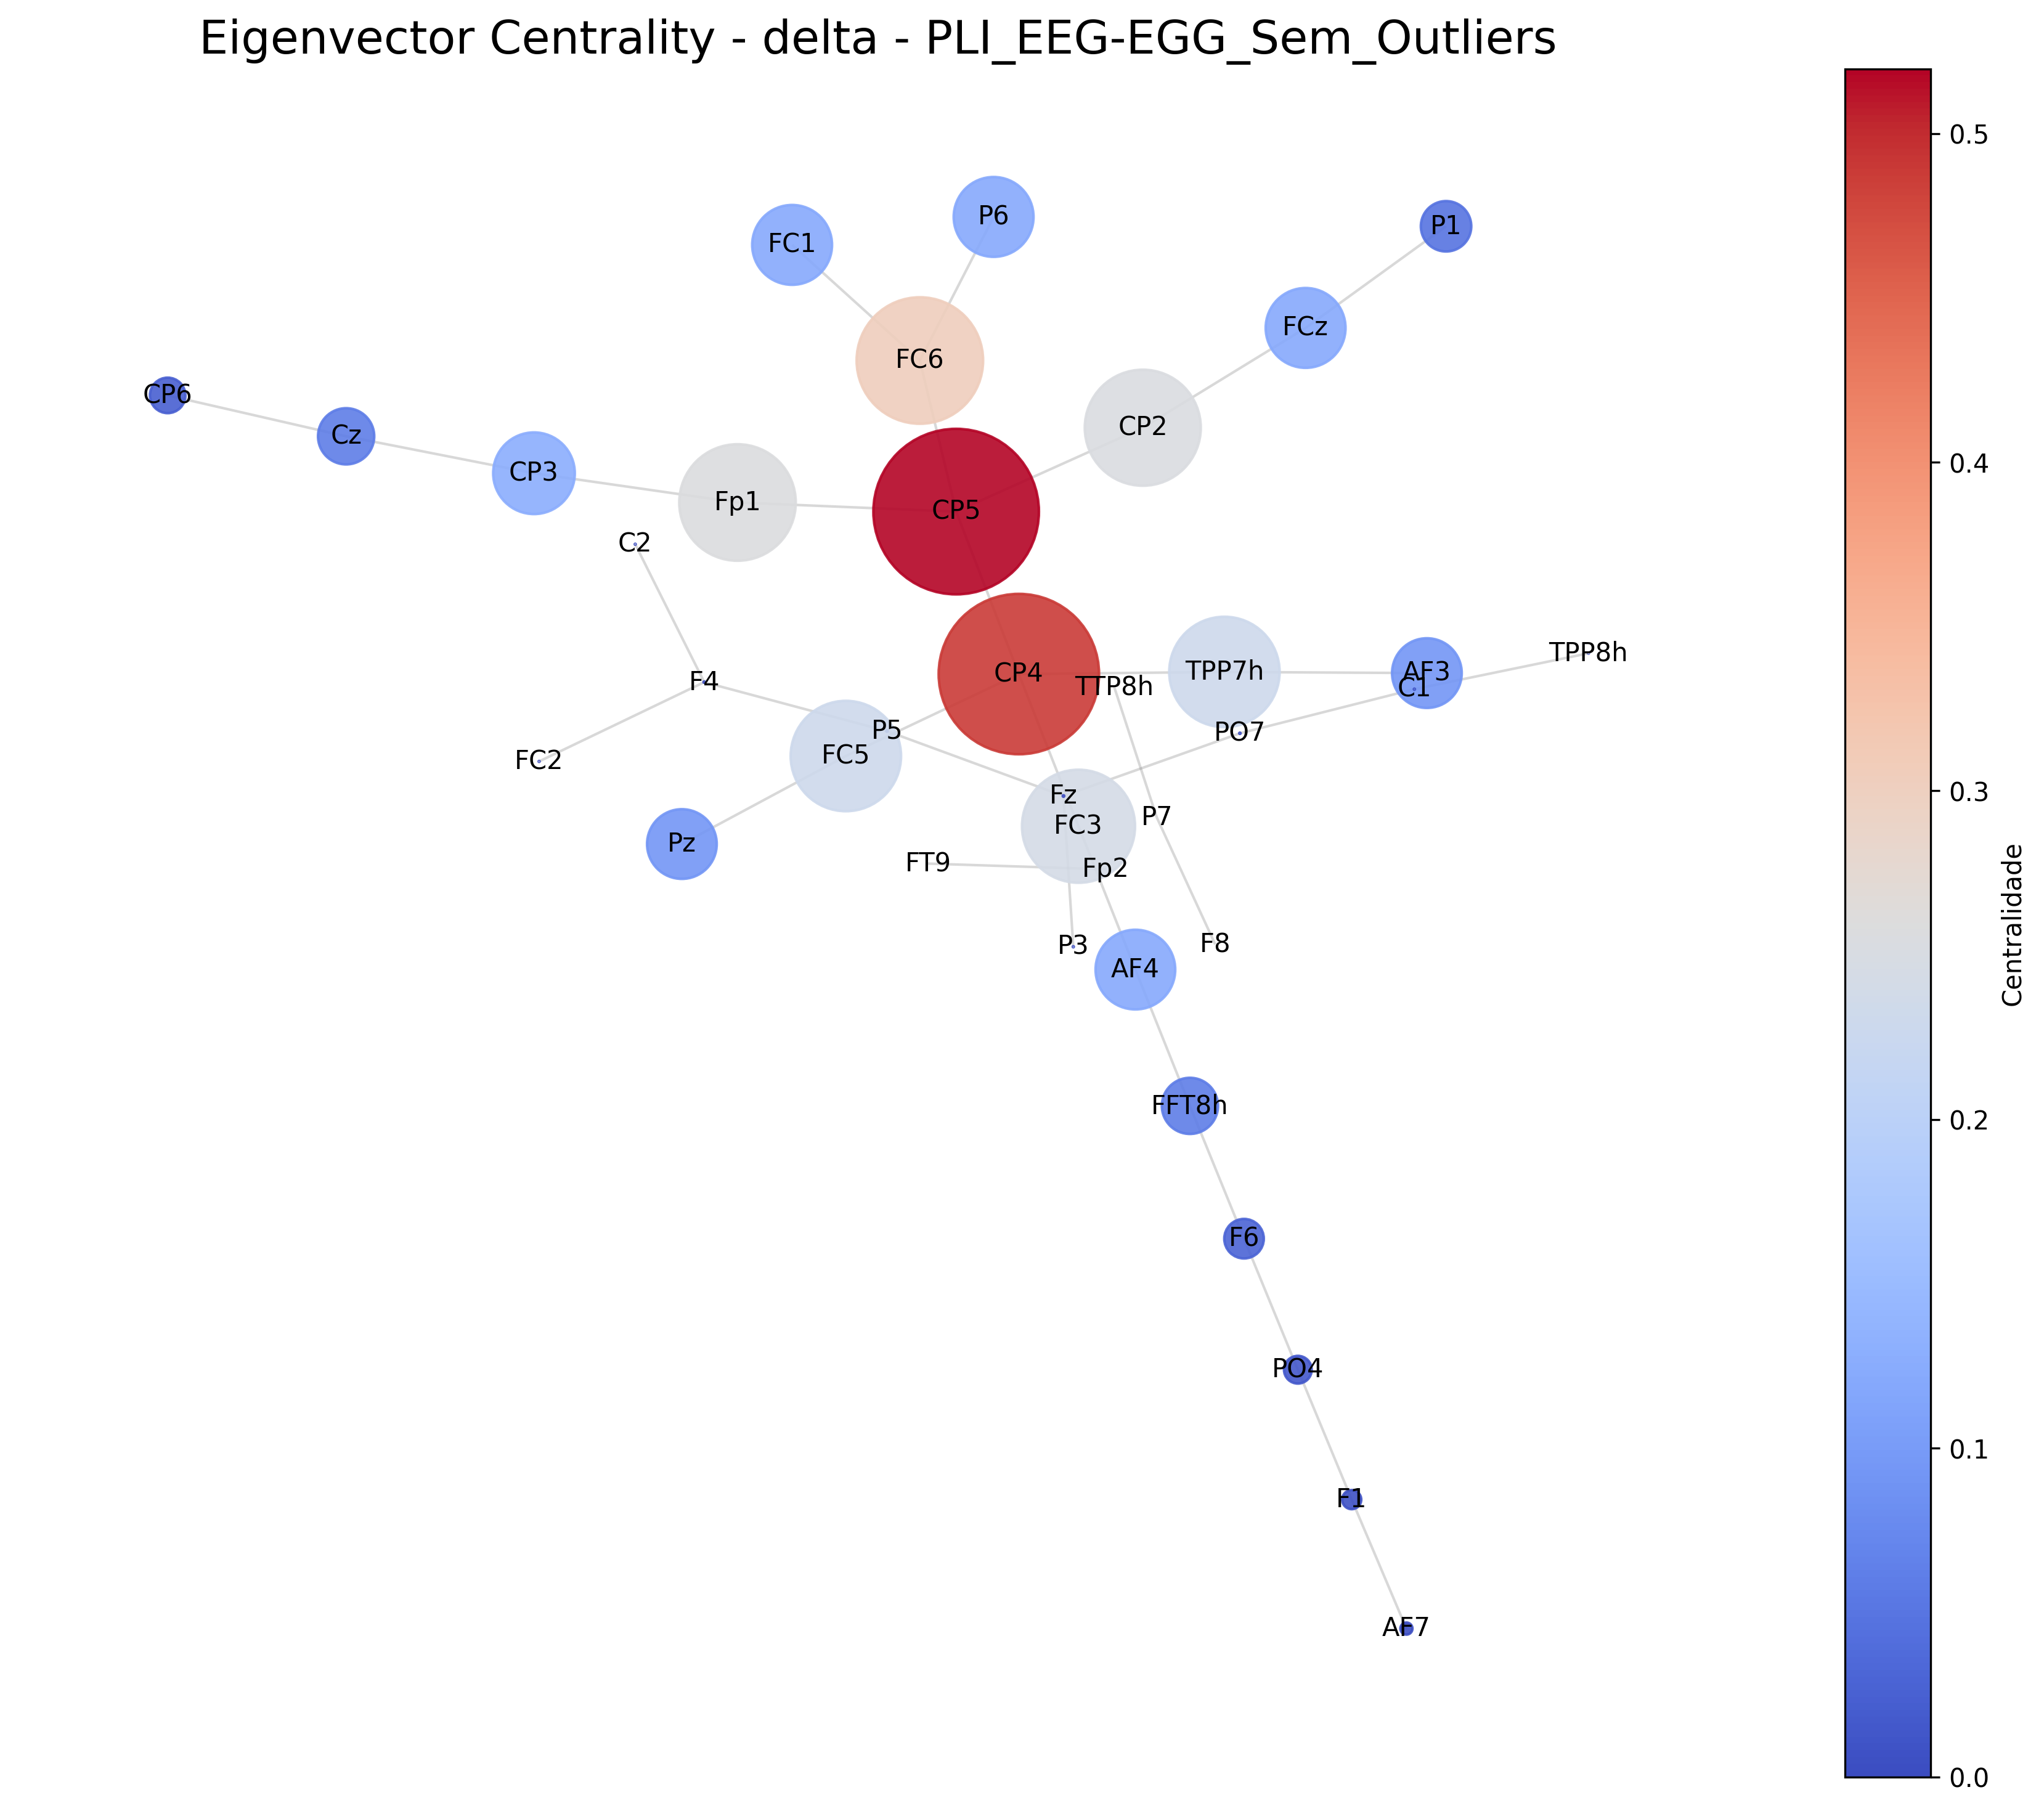
\includegraphics[width=0.45\textwidth]{figs/7_bootstrap_results_analysis/3_centrality_graphs/Sem_Outliers/Eigenvector_Centrality__delta__PLI_EEGEGG_Sem_Outliers.png}
    }
    \caption{\small \textbf{Eigenvector Centrality – Banda Delta (0.5--4 Hz):} A influência dos nodos muda após a remoção de outliers, com \textbf{CP5} emergindo como o principal na versão sem outliers.}
    \label{fig:eigenvector_delta}
\end{figure}

\subsection{Banda Gamma (30--60 Hz)}
\subsubsection{Betweenness Centrality}
\begin{figure}[H]
    \centering
    \subfloat[\small \textbf{Com Outliers:} Hierarquia – 1. \textbf{C5}; 2. \textbf{FFT8h, F3}; 3. \textbf{FT10, C1, CP4, P6}; 4. \textbf{Cz, C4, F1, Fp2, P5}.]{%
        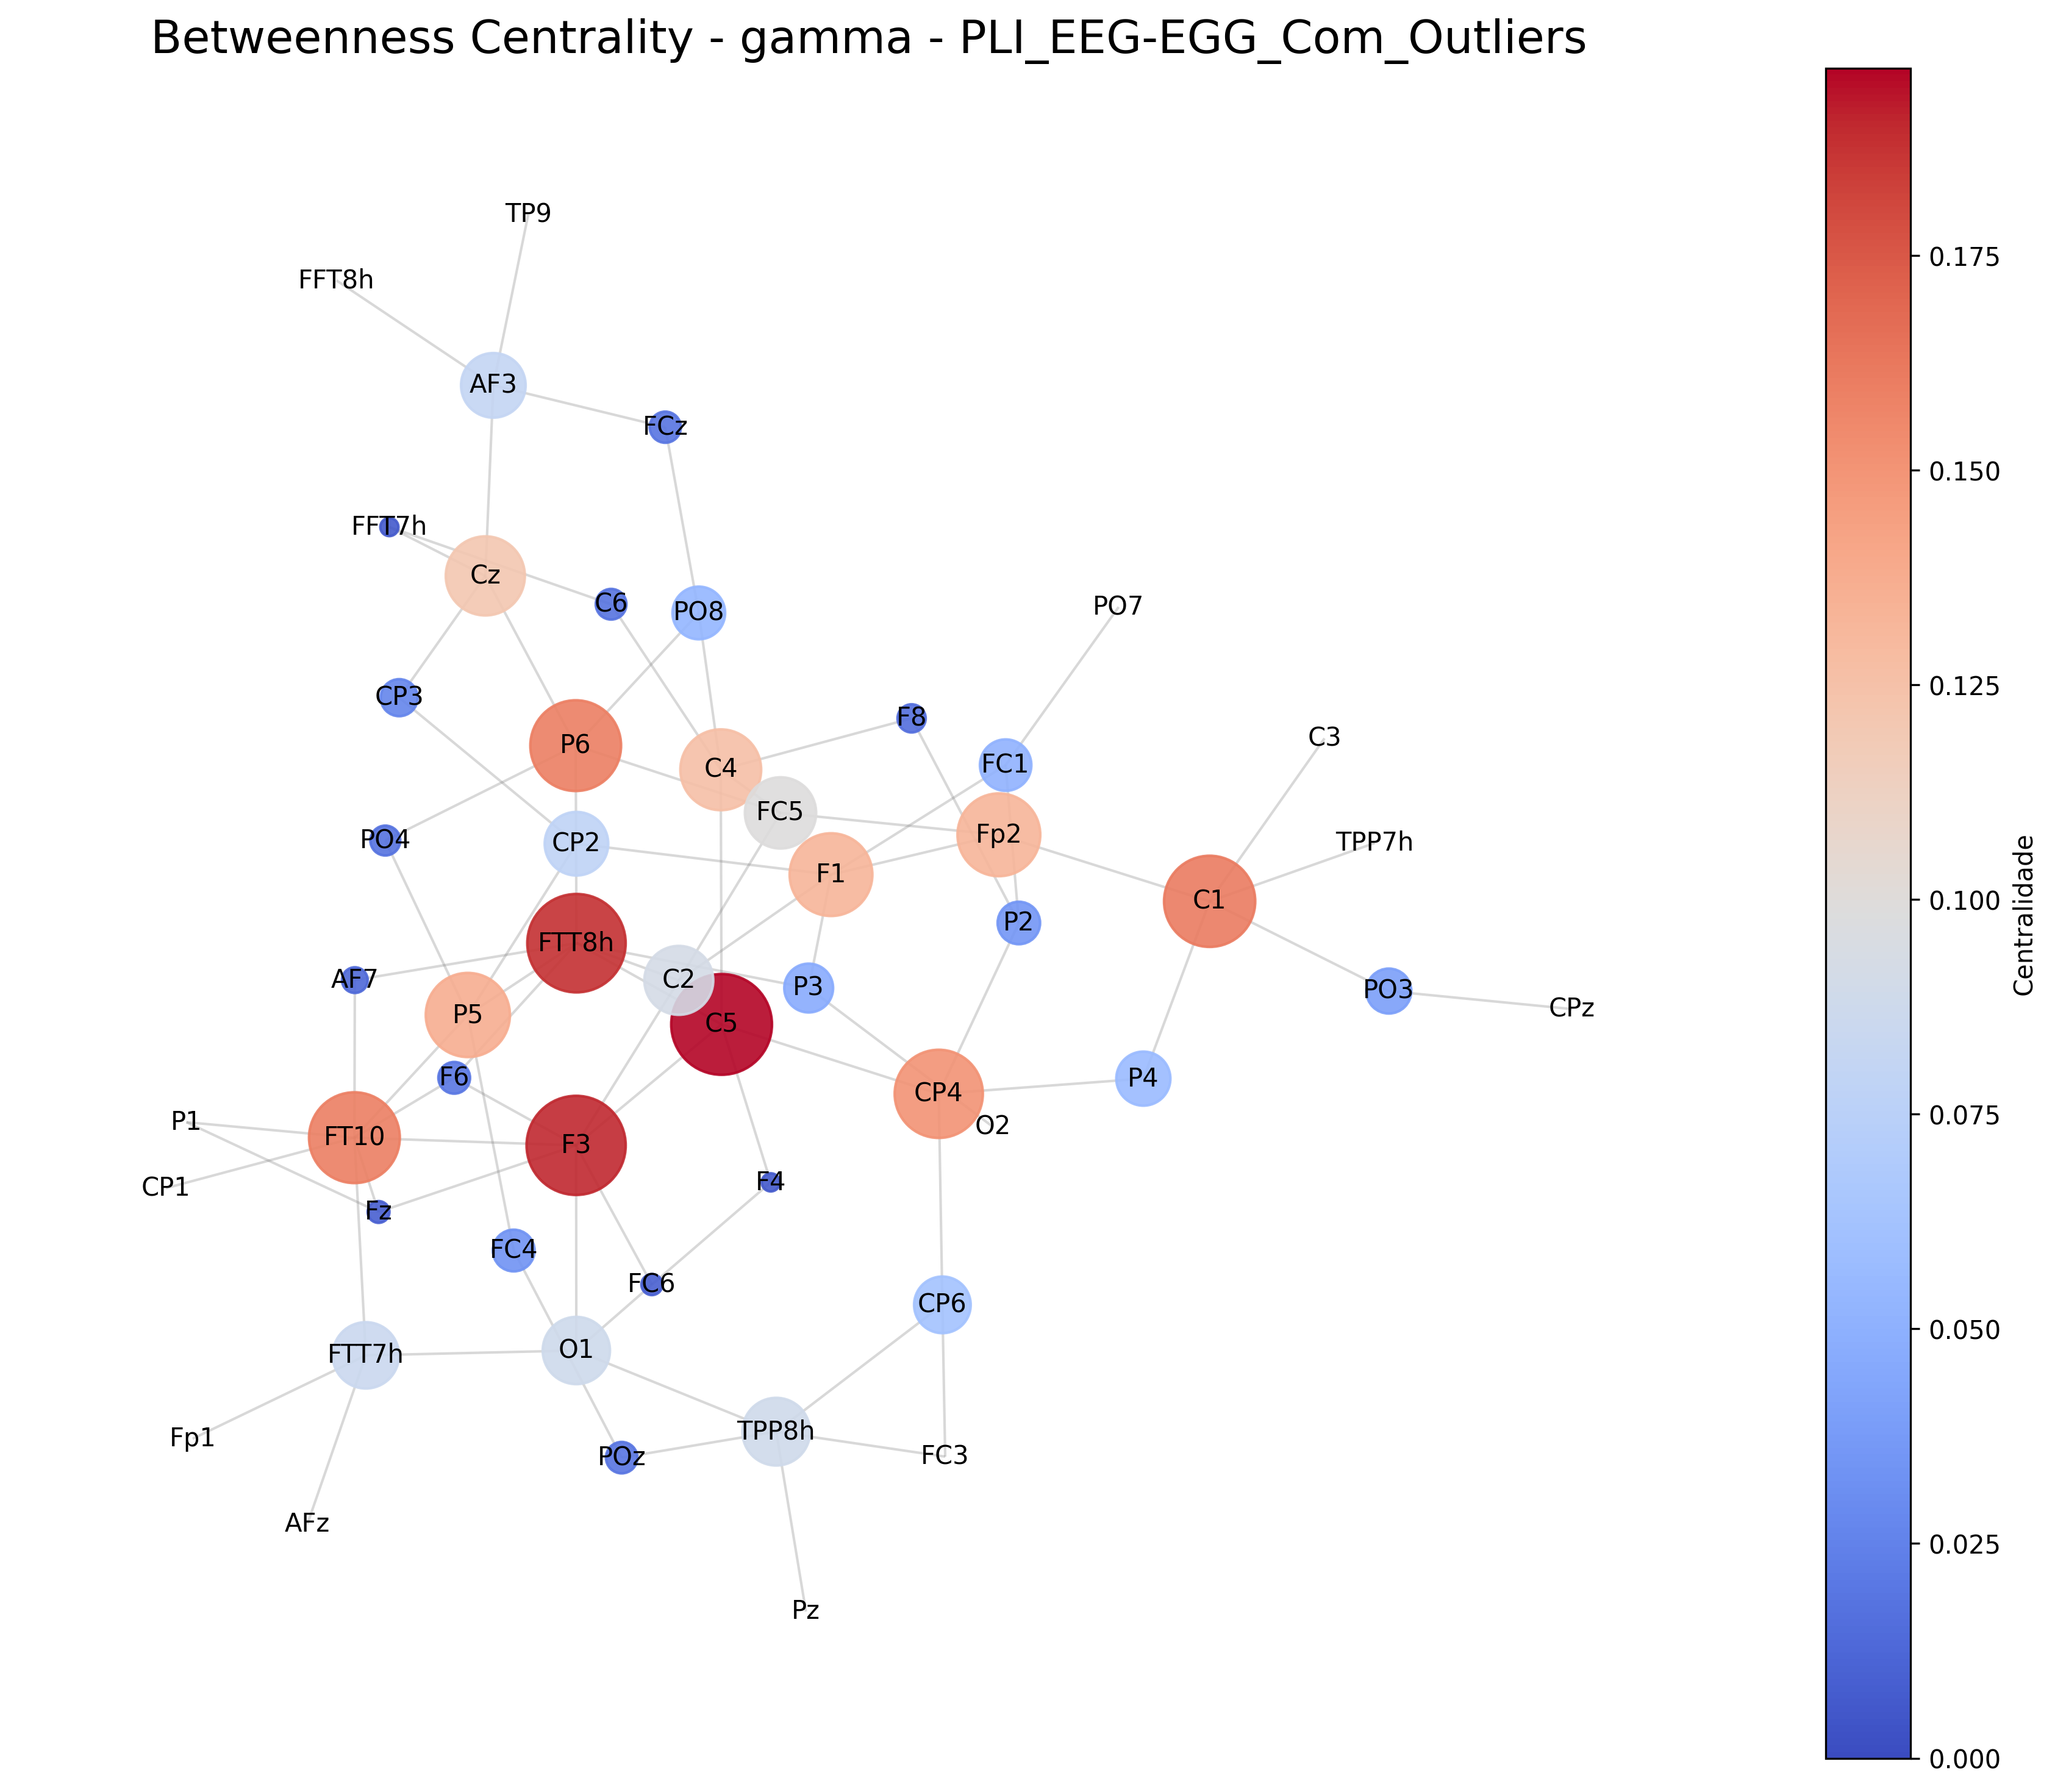
\includegraphics[width=0.45\textwidth]{figs/7_bootstrap_results_analysis/3_centrality_graphs/Com_Outliers/Betweenness_Centrality__gamma__PLI_EEGEGG_Com_Outliers.png}
    }
    \hfill
    \subfloat[\small \textbf{Sem Outliers:} Hierarquia – 1. \textbf{F3}; 2. \textbf{C5}; 3. \textbf{FFT8h, FT10}; 4. \textbf{P5}.]{%
        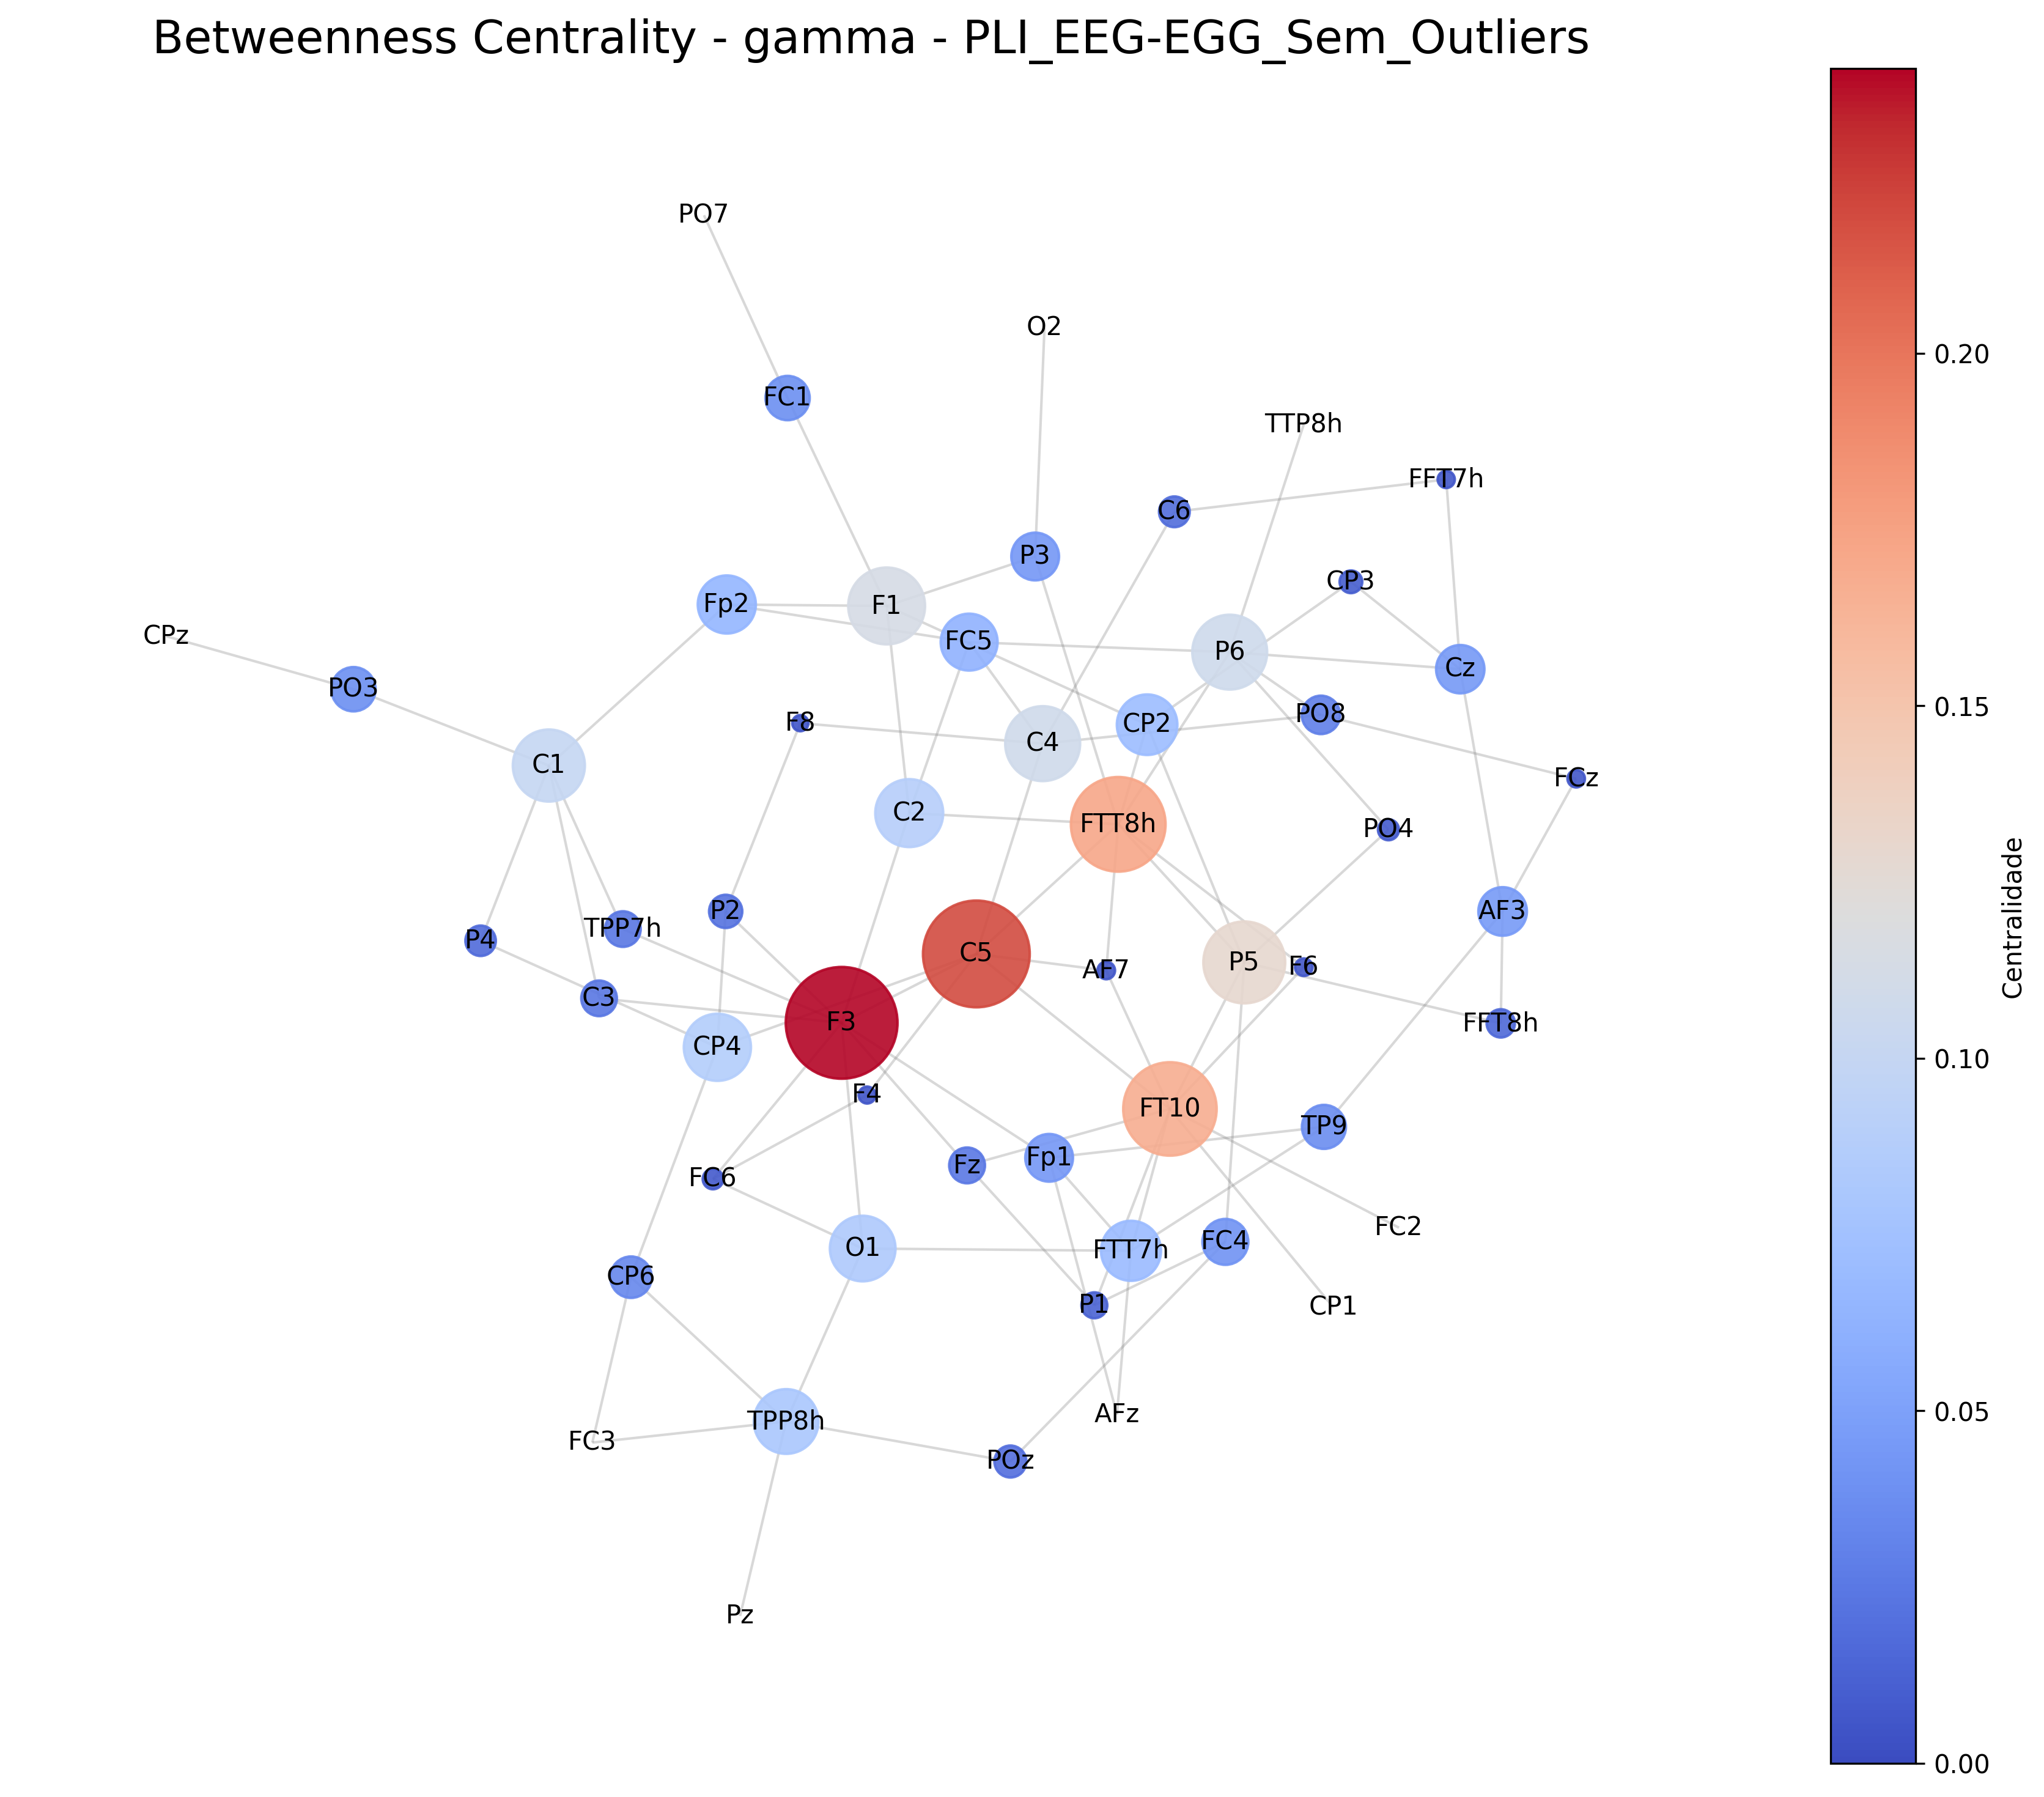
\includegraphics[width=0.45\textwidth]{figs/7_bootstrap_results_analysis/3_centrality_graphs/Sem_Outliers/Betweenness_Centrality__gamma__PLI_EEGEGG_Sem_Outliers.png}
    }
    \caption{\small \textbf{Betweenness Centrality – Banda Gamma (30--60 Hz):} A hierarquia dos canais na rede gamma apresenta uma divisão mais complexa, com uma diminuição geral dos valores na versão sem outliers.}
    \label{fig:betweenness_gamma}
\end{figure}

\subsubsection{Degree Centrality}
\begin{figure}[H]
    \centering
    \subfloat[\small \textbf{Com Outliers:} Hierarquia – 1. \textbf{FT10}; 2. \textbf{FTT8h}; 3. \textbf{F3}; 4. \textbf{P5, P6, C4, F1, C5, C1, TPP8h}.]{%
        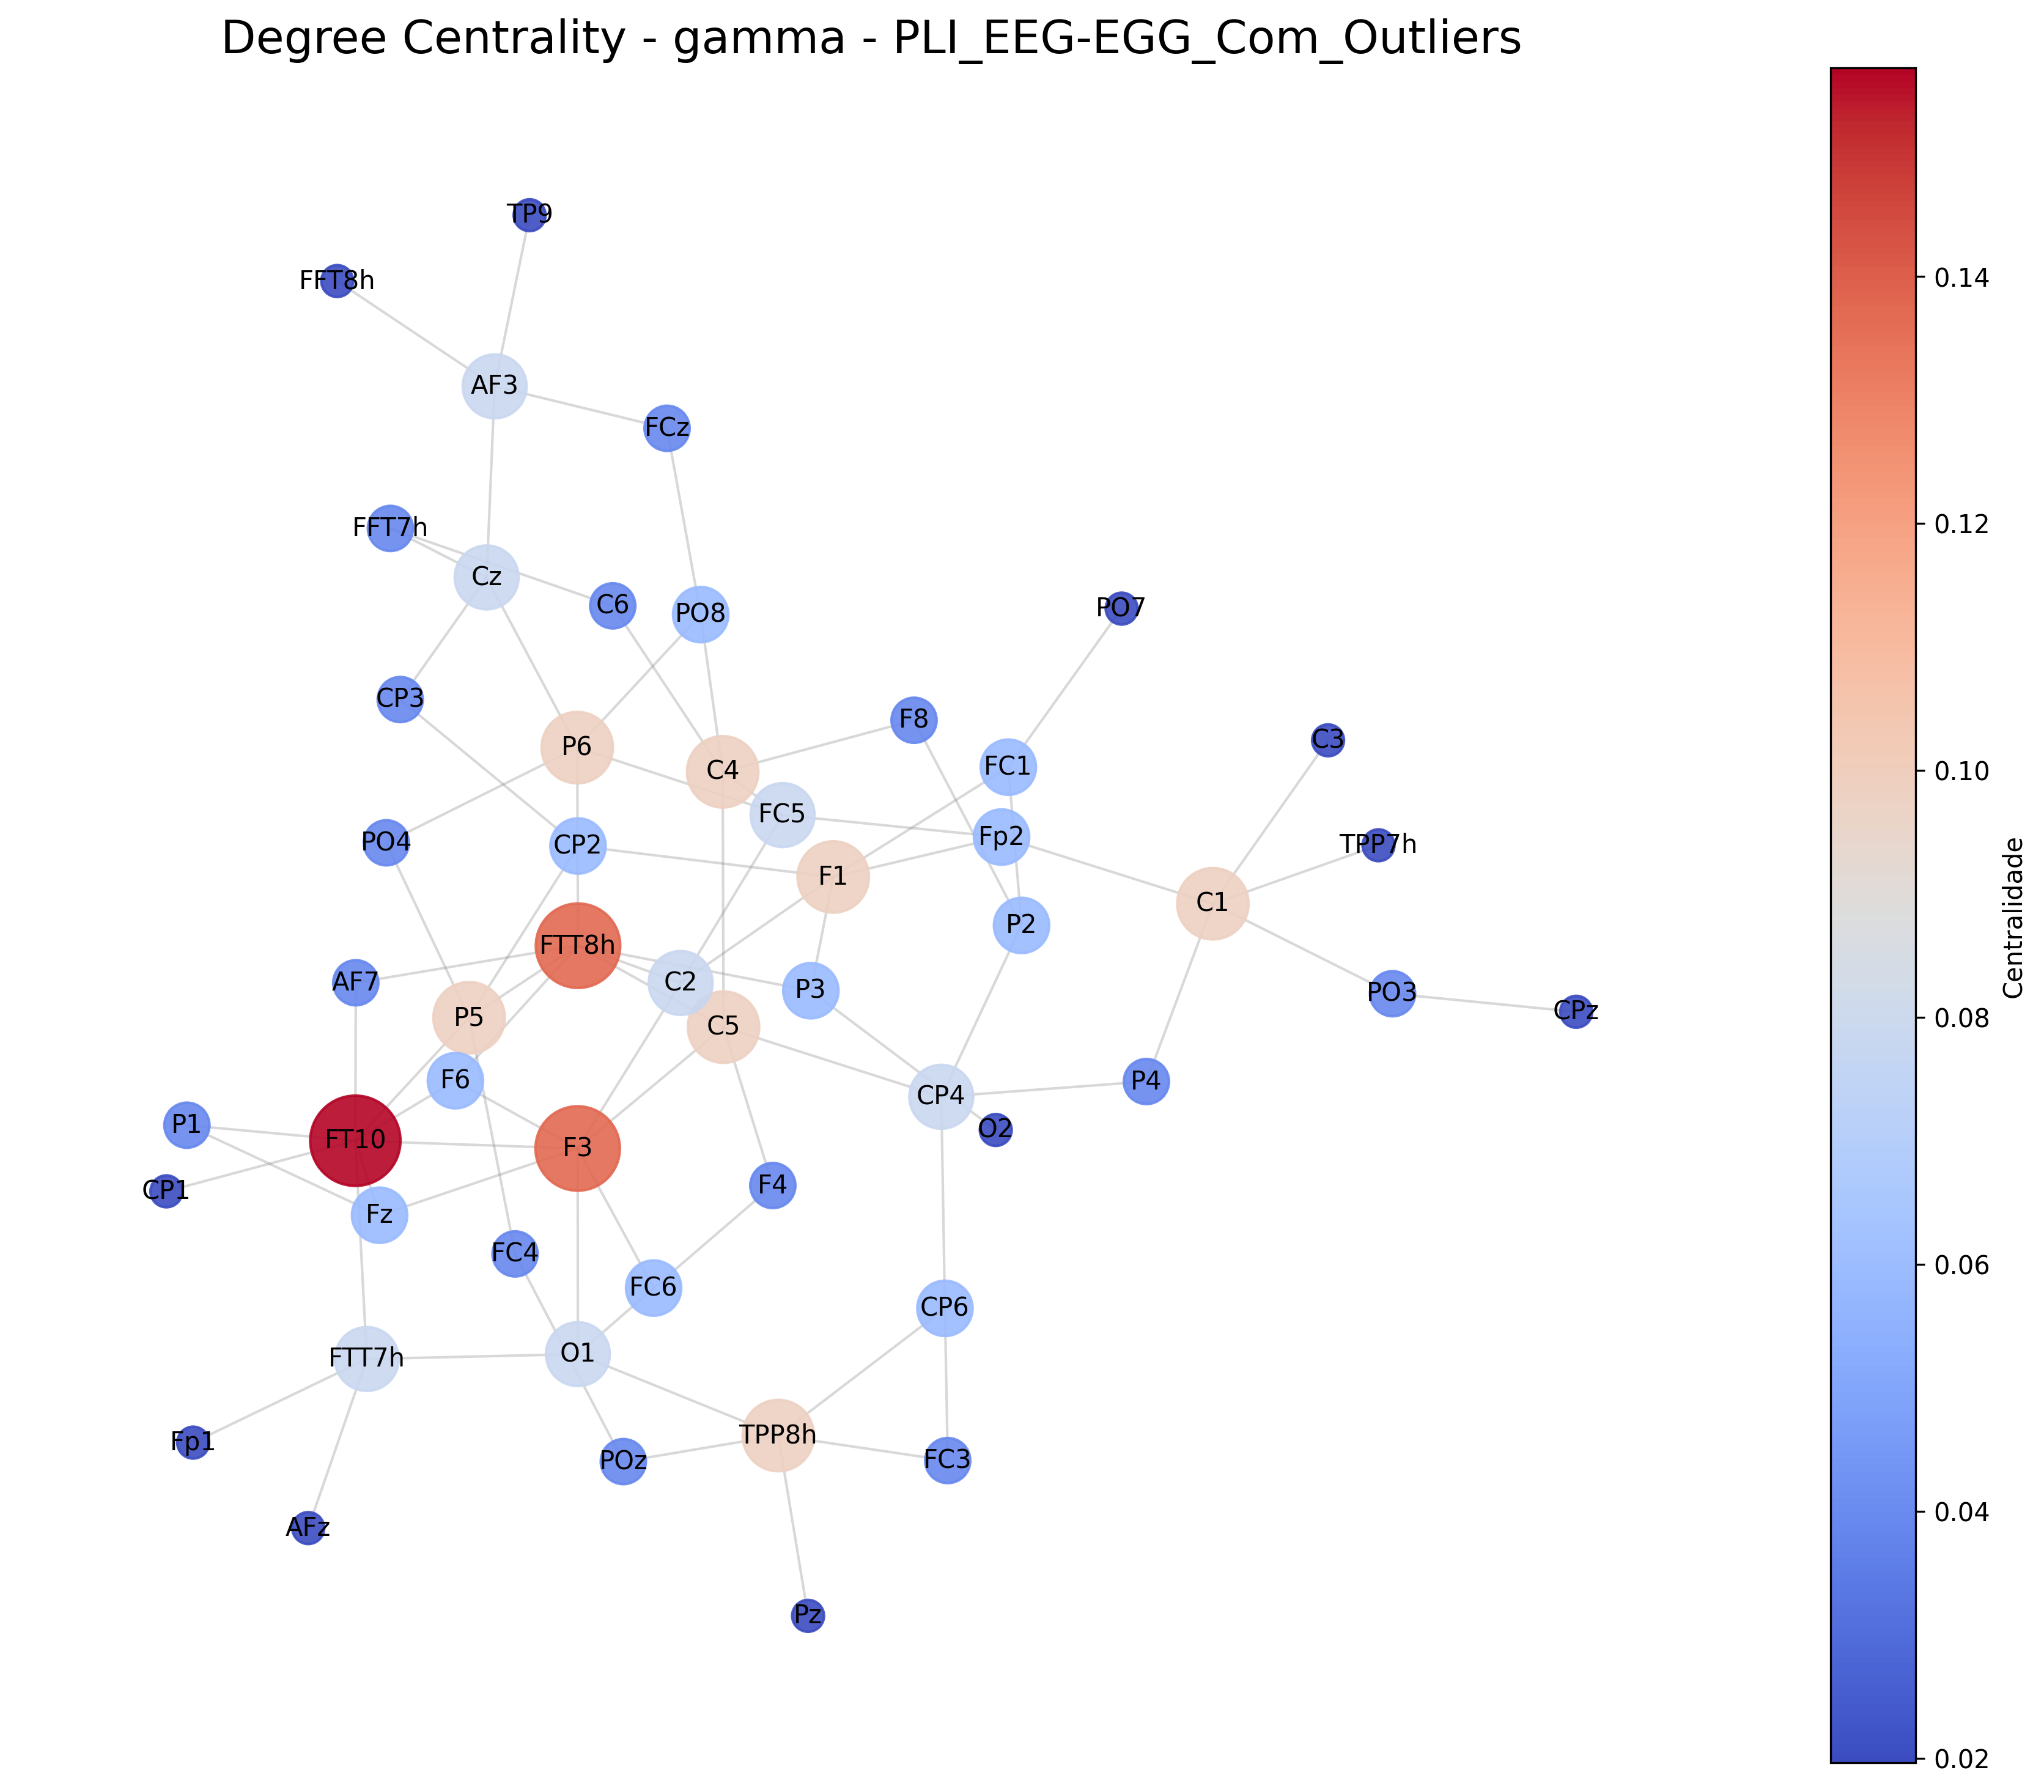
\includegraphics[width=0.45\textwidth]{figs/7_bootstrap_results_analysis/3_centrality_graphs/Com_Outliers/Degree_Centrality__gamma__PLI_EEGEGG_Com_Outliers.png}
    }
    \hfill
    \subfloat[\small \textbf{Sem Outliers:} Hierarquia – 1. \textbf{F3, FT10}; 2. \textbf{FTT8h}; 3. \textbf{C5}; 4. \textbf{P5, P6}.]{%
        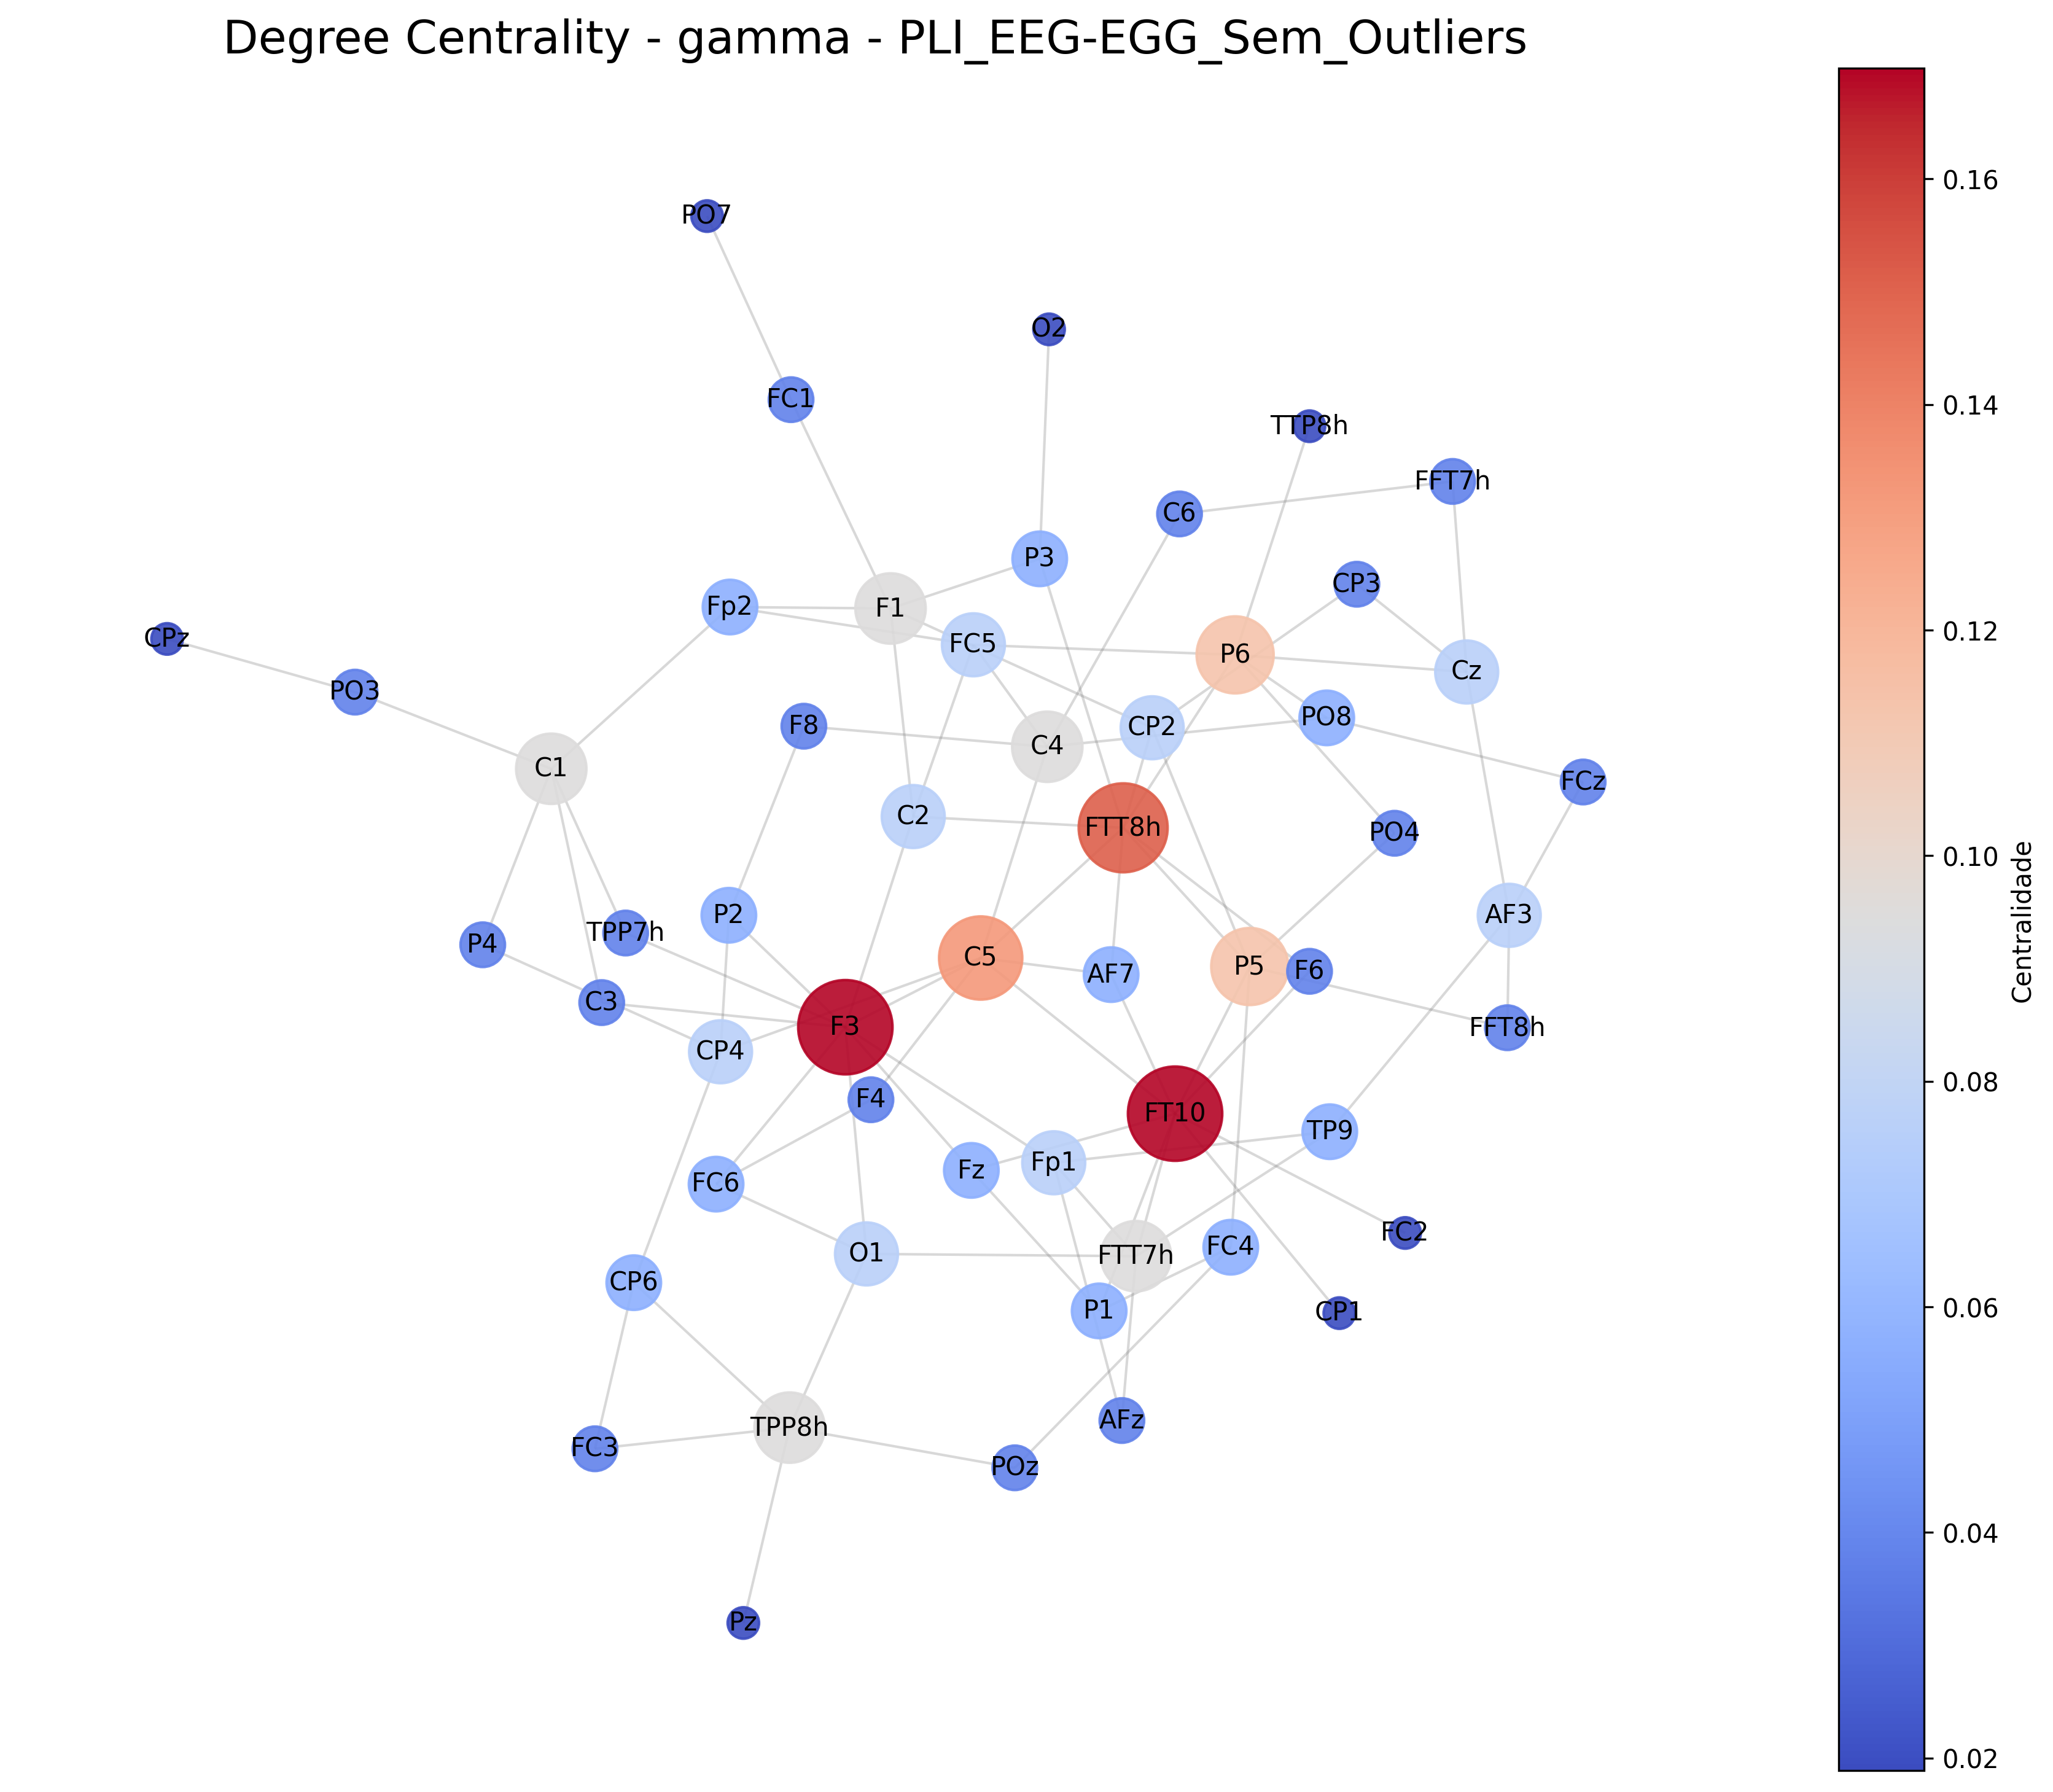
\includegraphics[width=0.45\textwidth]{figs/7_bootstrap_results_analysis/3_centrality_graphs/Sem_Outliers/Degree_Centrality__gamma__PLI_EEGEGG_Sem_Outliers.png}
    }
    \caption{\small \textbf{Degree Centrality – Banda Gamma (30--60 Hz):} Os canais de maior conectividade direta mudam levemente entre os cenários, com uma hierarquia consistente na versão sem outliers.}
    \label{fig:degree_gamma}
\end{figure}

\subsubsection{Eigenvector Centrality}
\begin{figure}[H]
    \centering
    \subfloat[\small \textbf{Com Outliers:} Hierarquia – 1. \textbf{F3, FT10}; 2. \textbf{FTT8h}; 3. \textbf{F6}; 4. \textbf{Fz, P5, C2, C5}.]{%
        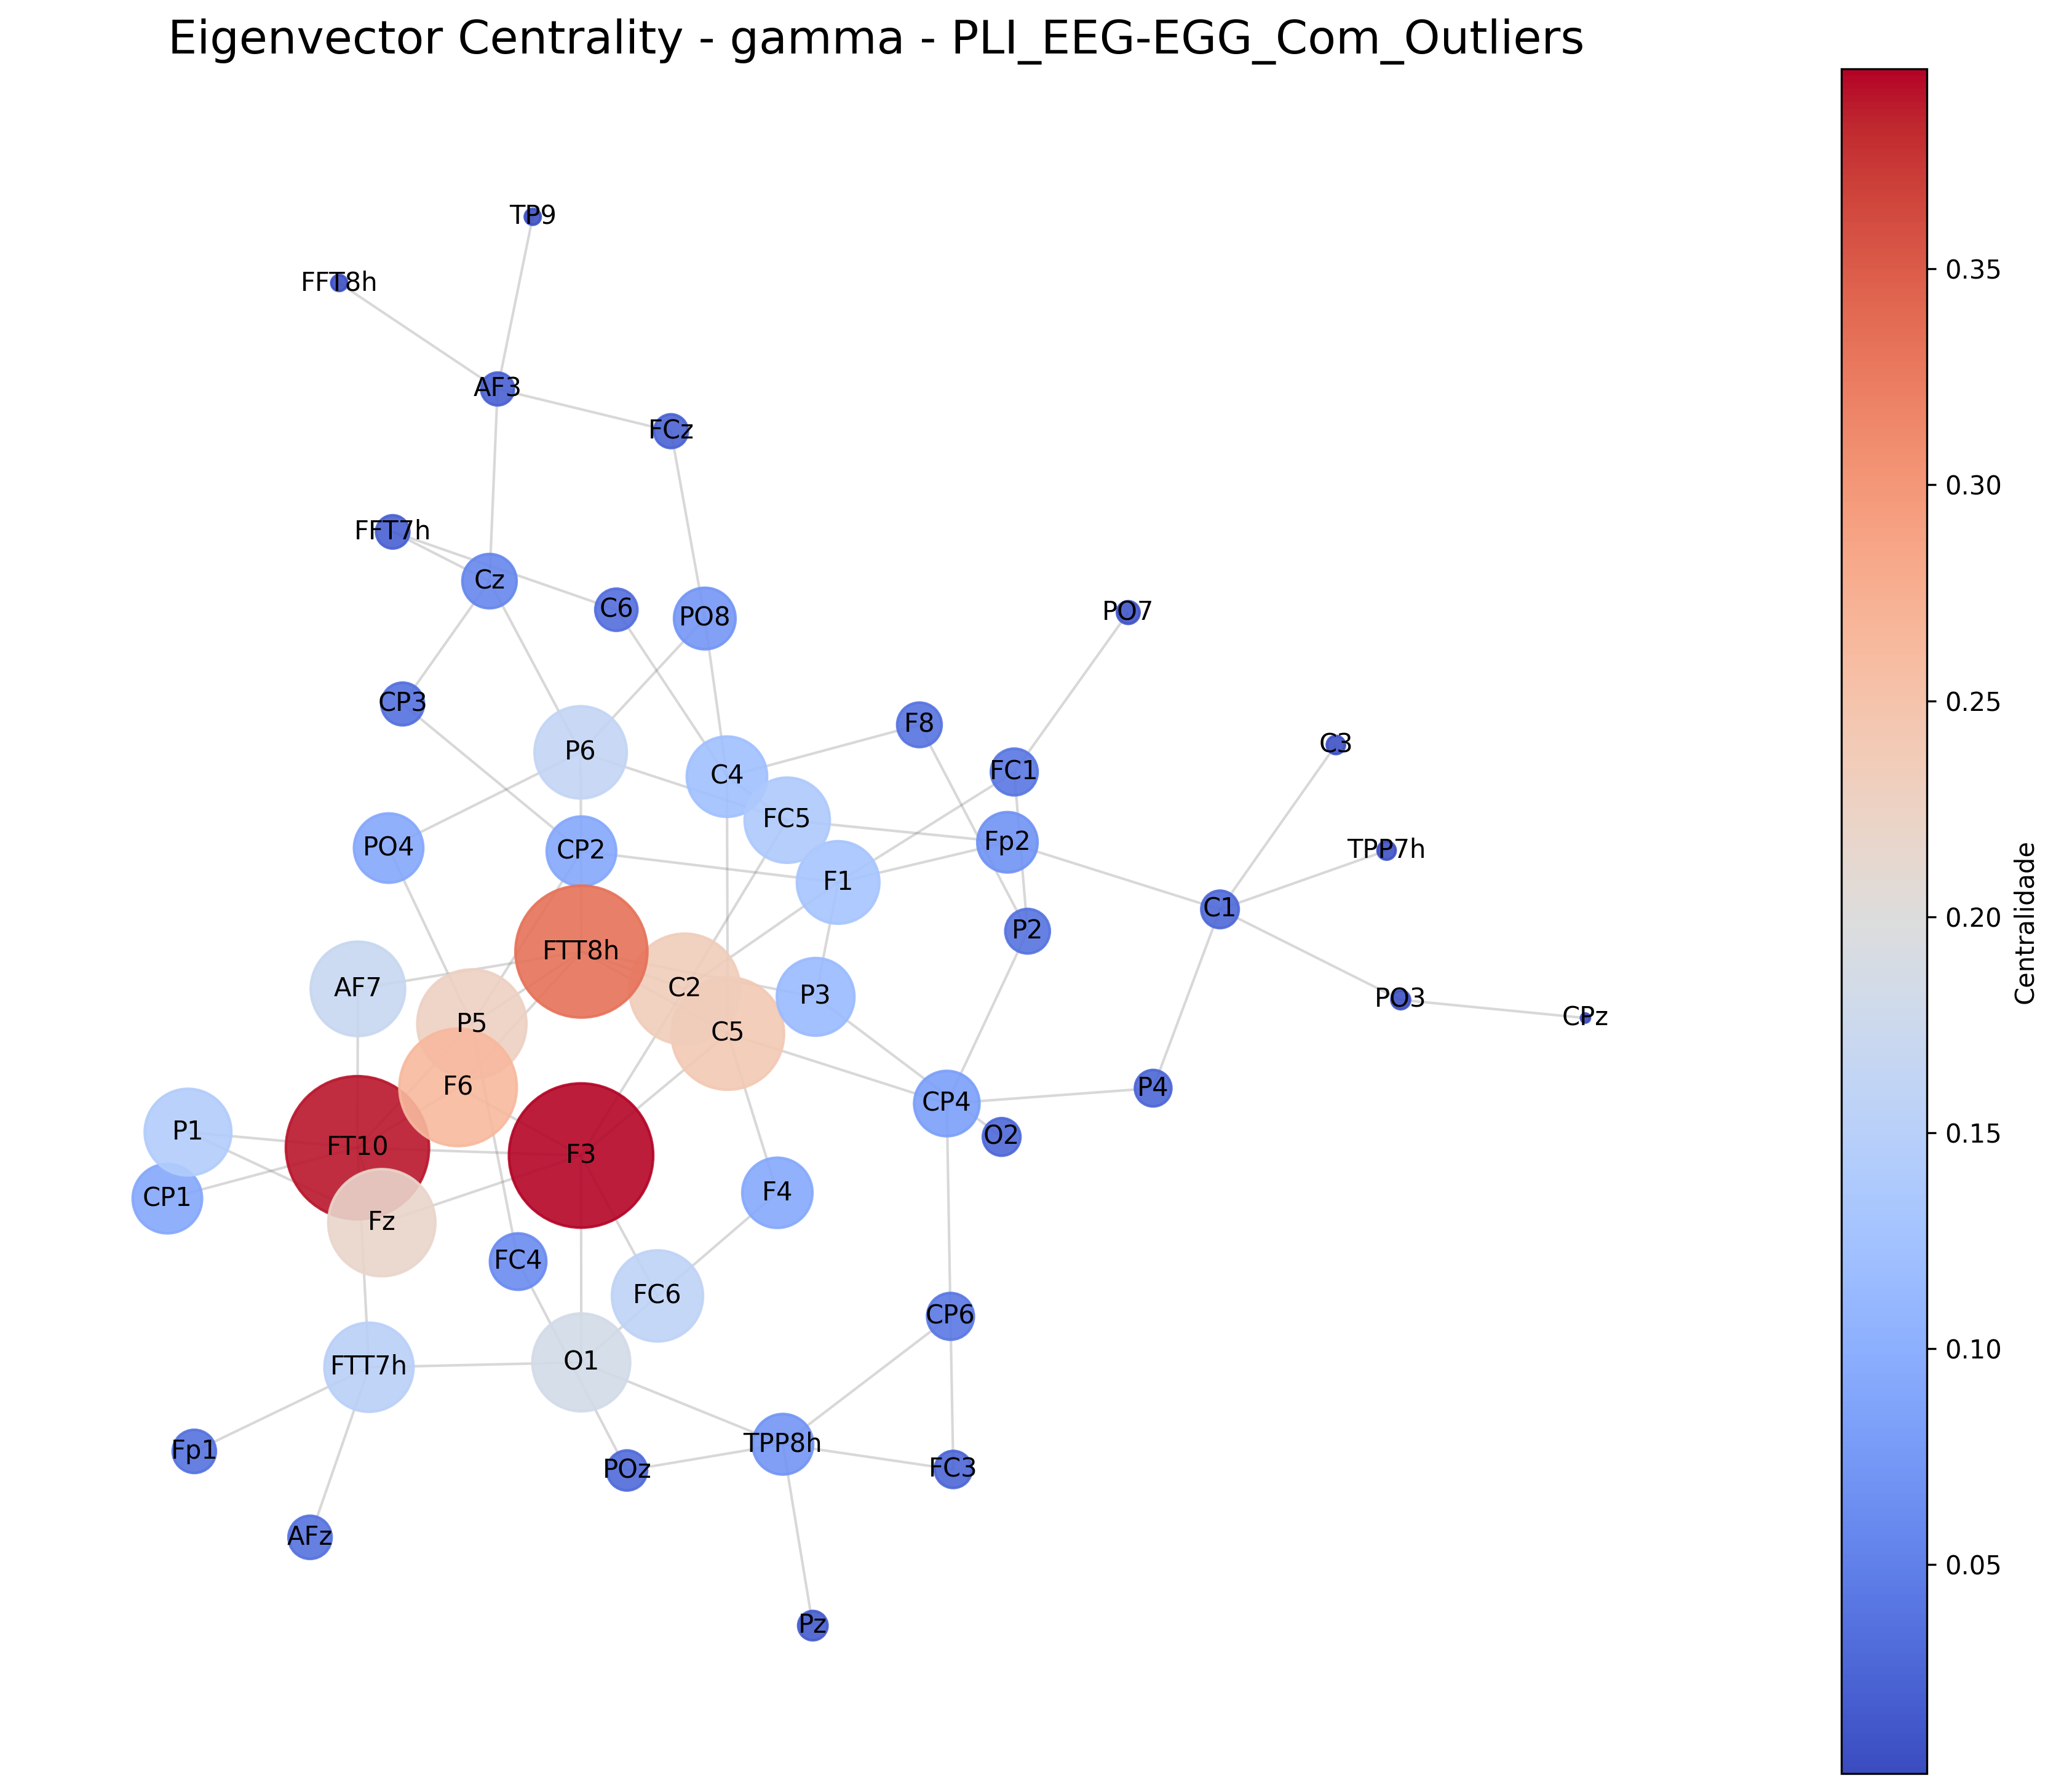
\includegraphics[width=0.45\textwidth]{figs/7_bootstrap_results_analysis/3_centrality_graphs/Com_Outliers/Eigenvector_Centrality__gamma__PLI_EEGEGG_Com_Outliers.png}
    }
    \hfill
    \subfloat[\small \textbf{Sem Outliers:} Hierarquia – 1. \textbf{FTT8h, C5, FT10}; 2. \textbf{F3}; 3. \textbf{P5}; 4. \textbf{AF7}; 5. \textbf{C2}.]{%
        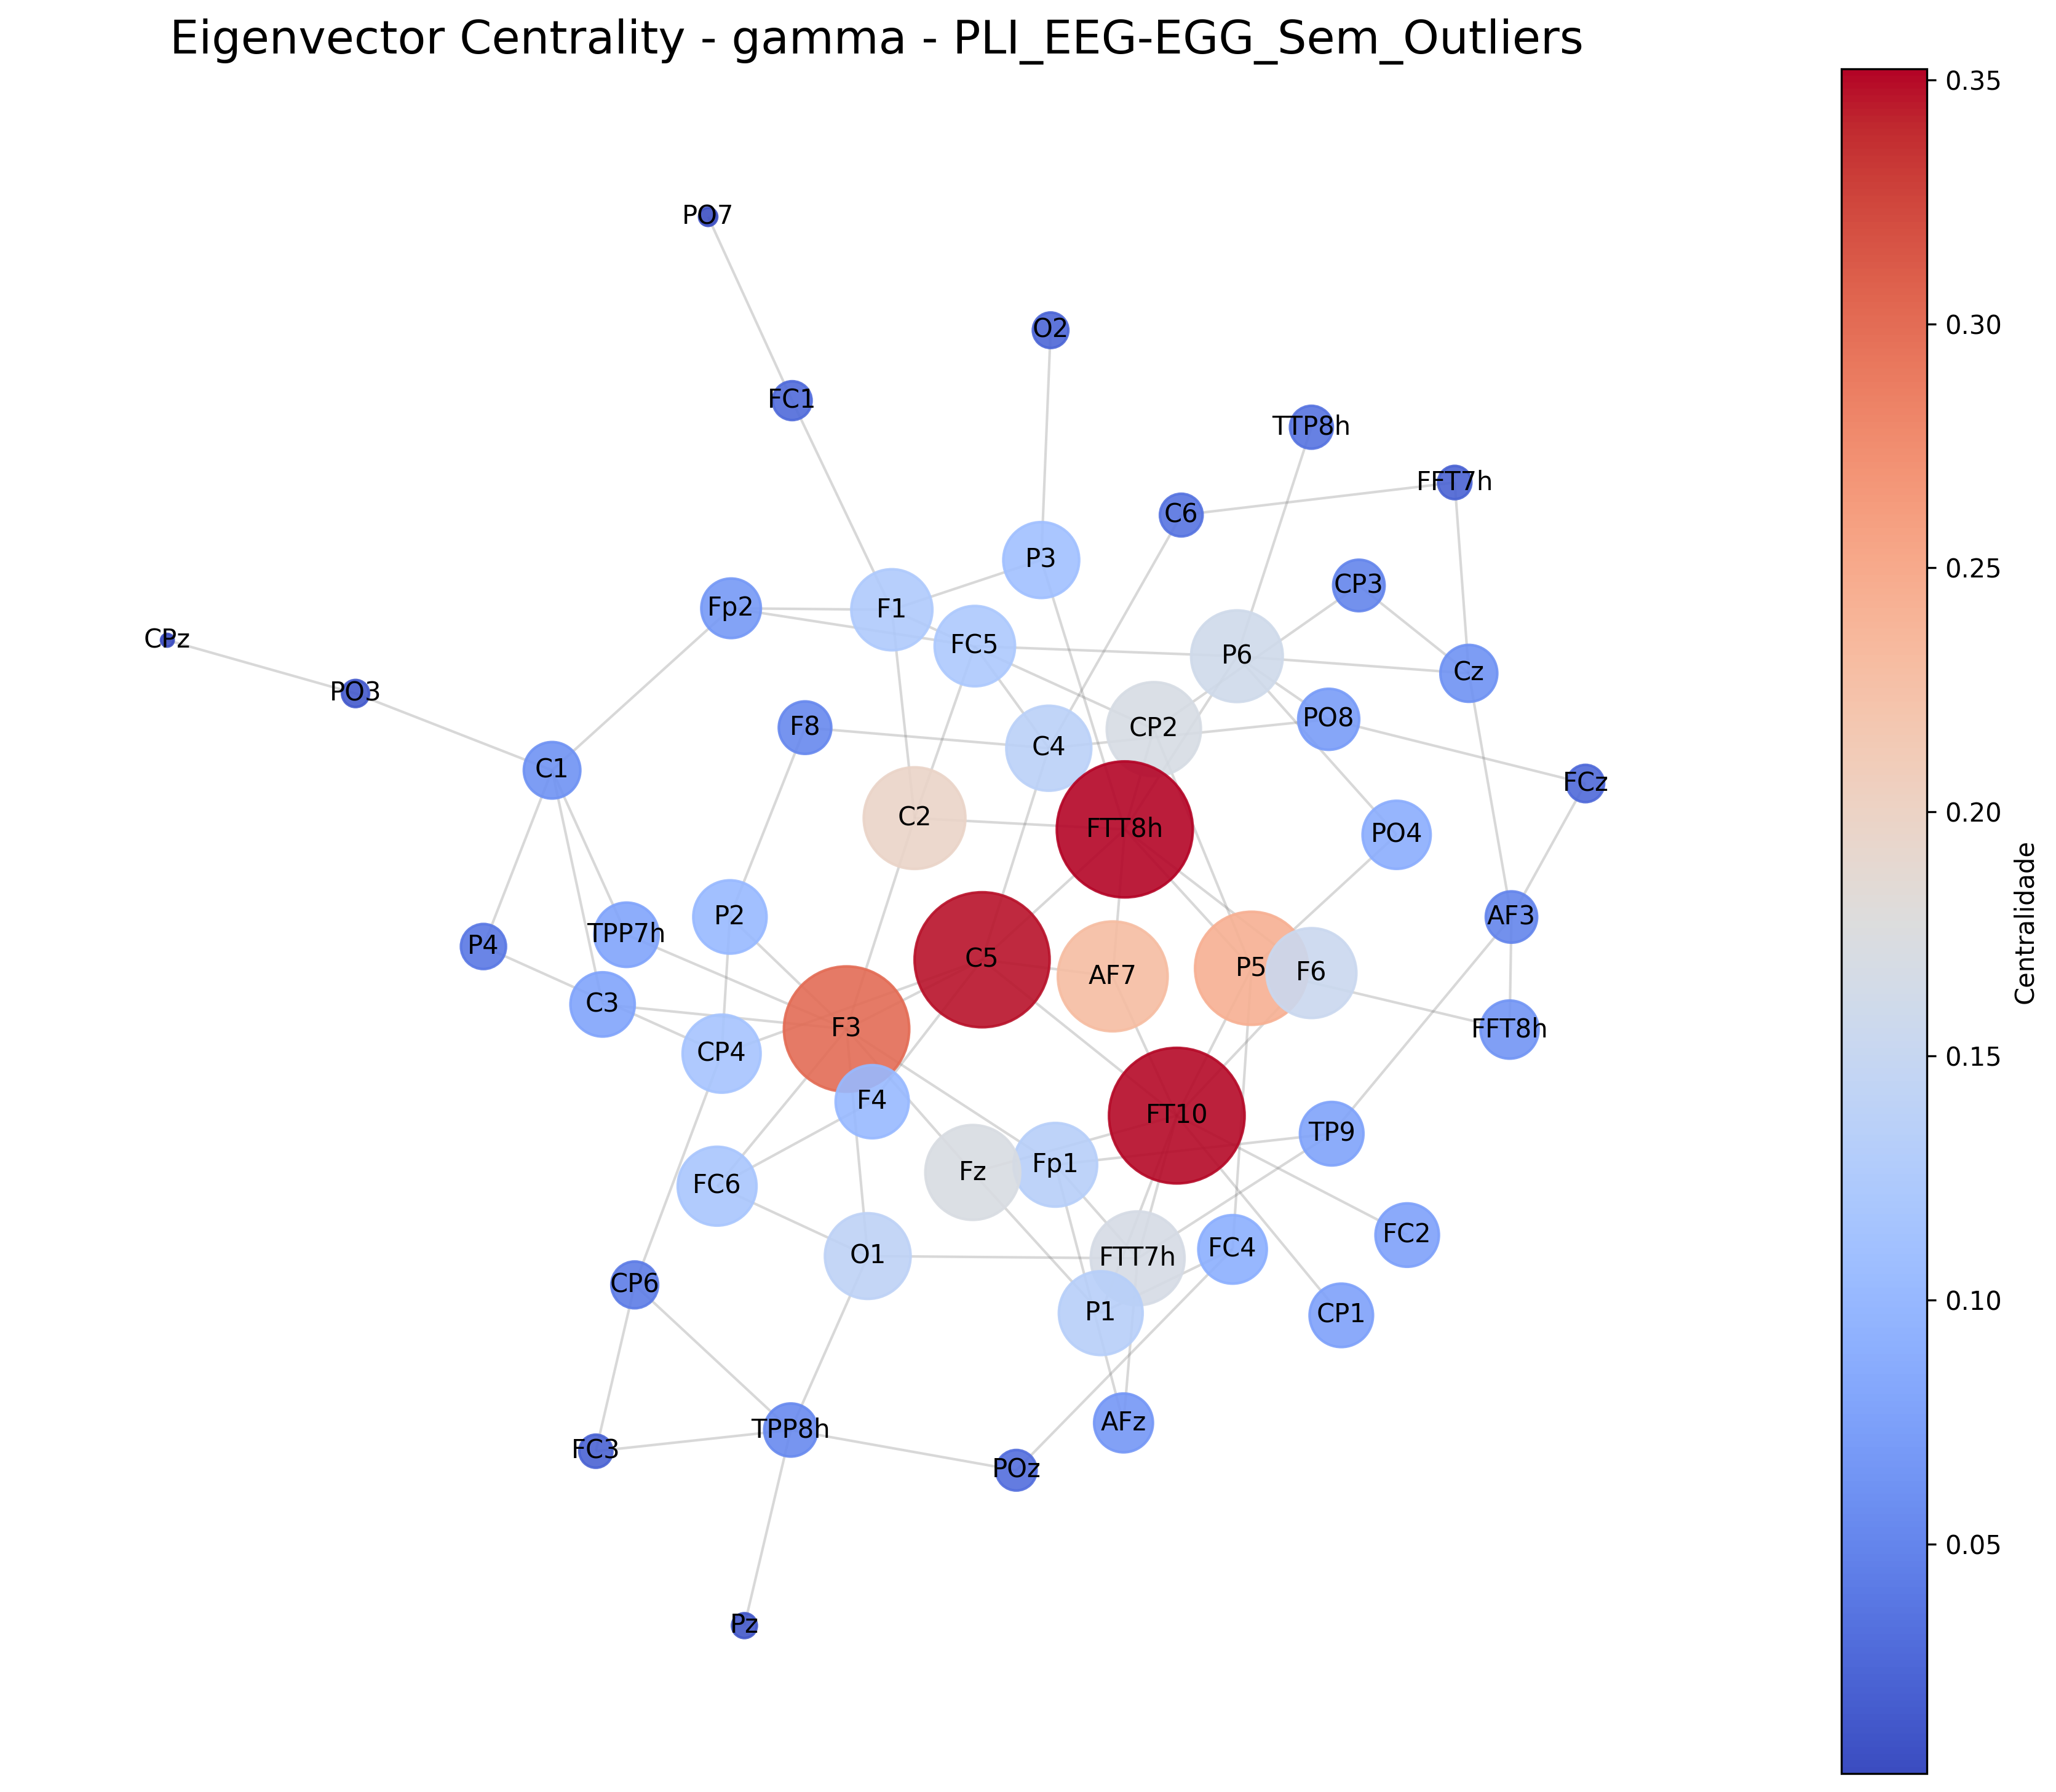
\includegraphics[width=0.45\textwidth]{figs/7_bootstrap_results_analysis/3_centrality_graphs/Sem_Outliers/Eigenvector_Centrality__gamma__PLI_EEGEGG_Sem_Outliers.png}
    }
    \caption{\small \textbf{Eigenvector Centrality – Banda Gamma (30--60 Hz):} A influência dos canais na rede gamma apresenta uma leve reorganização após a remoção dos outliers.}
    \label{fig:eigenvector_gamma}
\end{figure}

\subsection{Banda Theta (4--8 Hz)}
\subsubsection{Betweenness Centrality}
\begin{figure}[H]
    \centering
    \subfloat[\small \textbf{Com Outliers:} Hierarquia – 1. \textbf{FC1, PO4}; 2. \textbf{F8}; 3. \textbf{Fp2}; 4. \textbf{CP3, C1}.]{%
        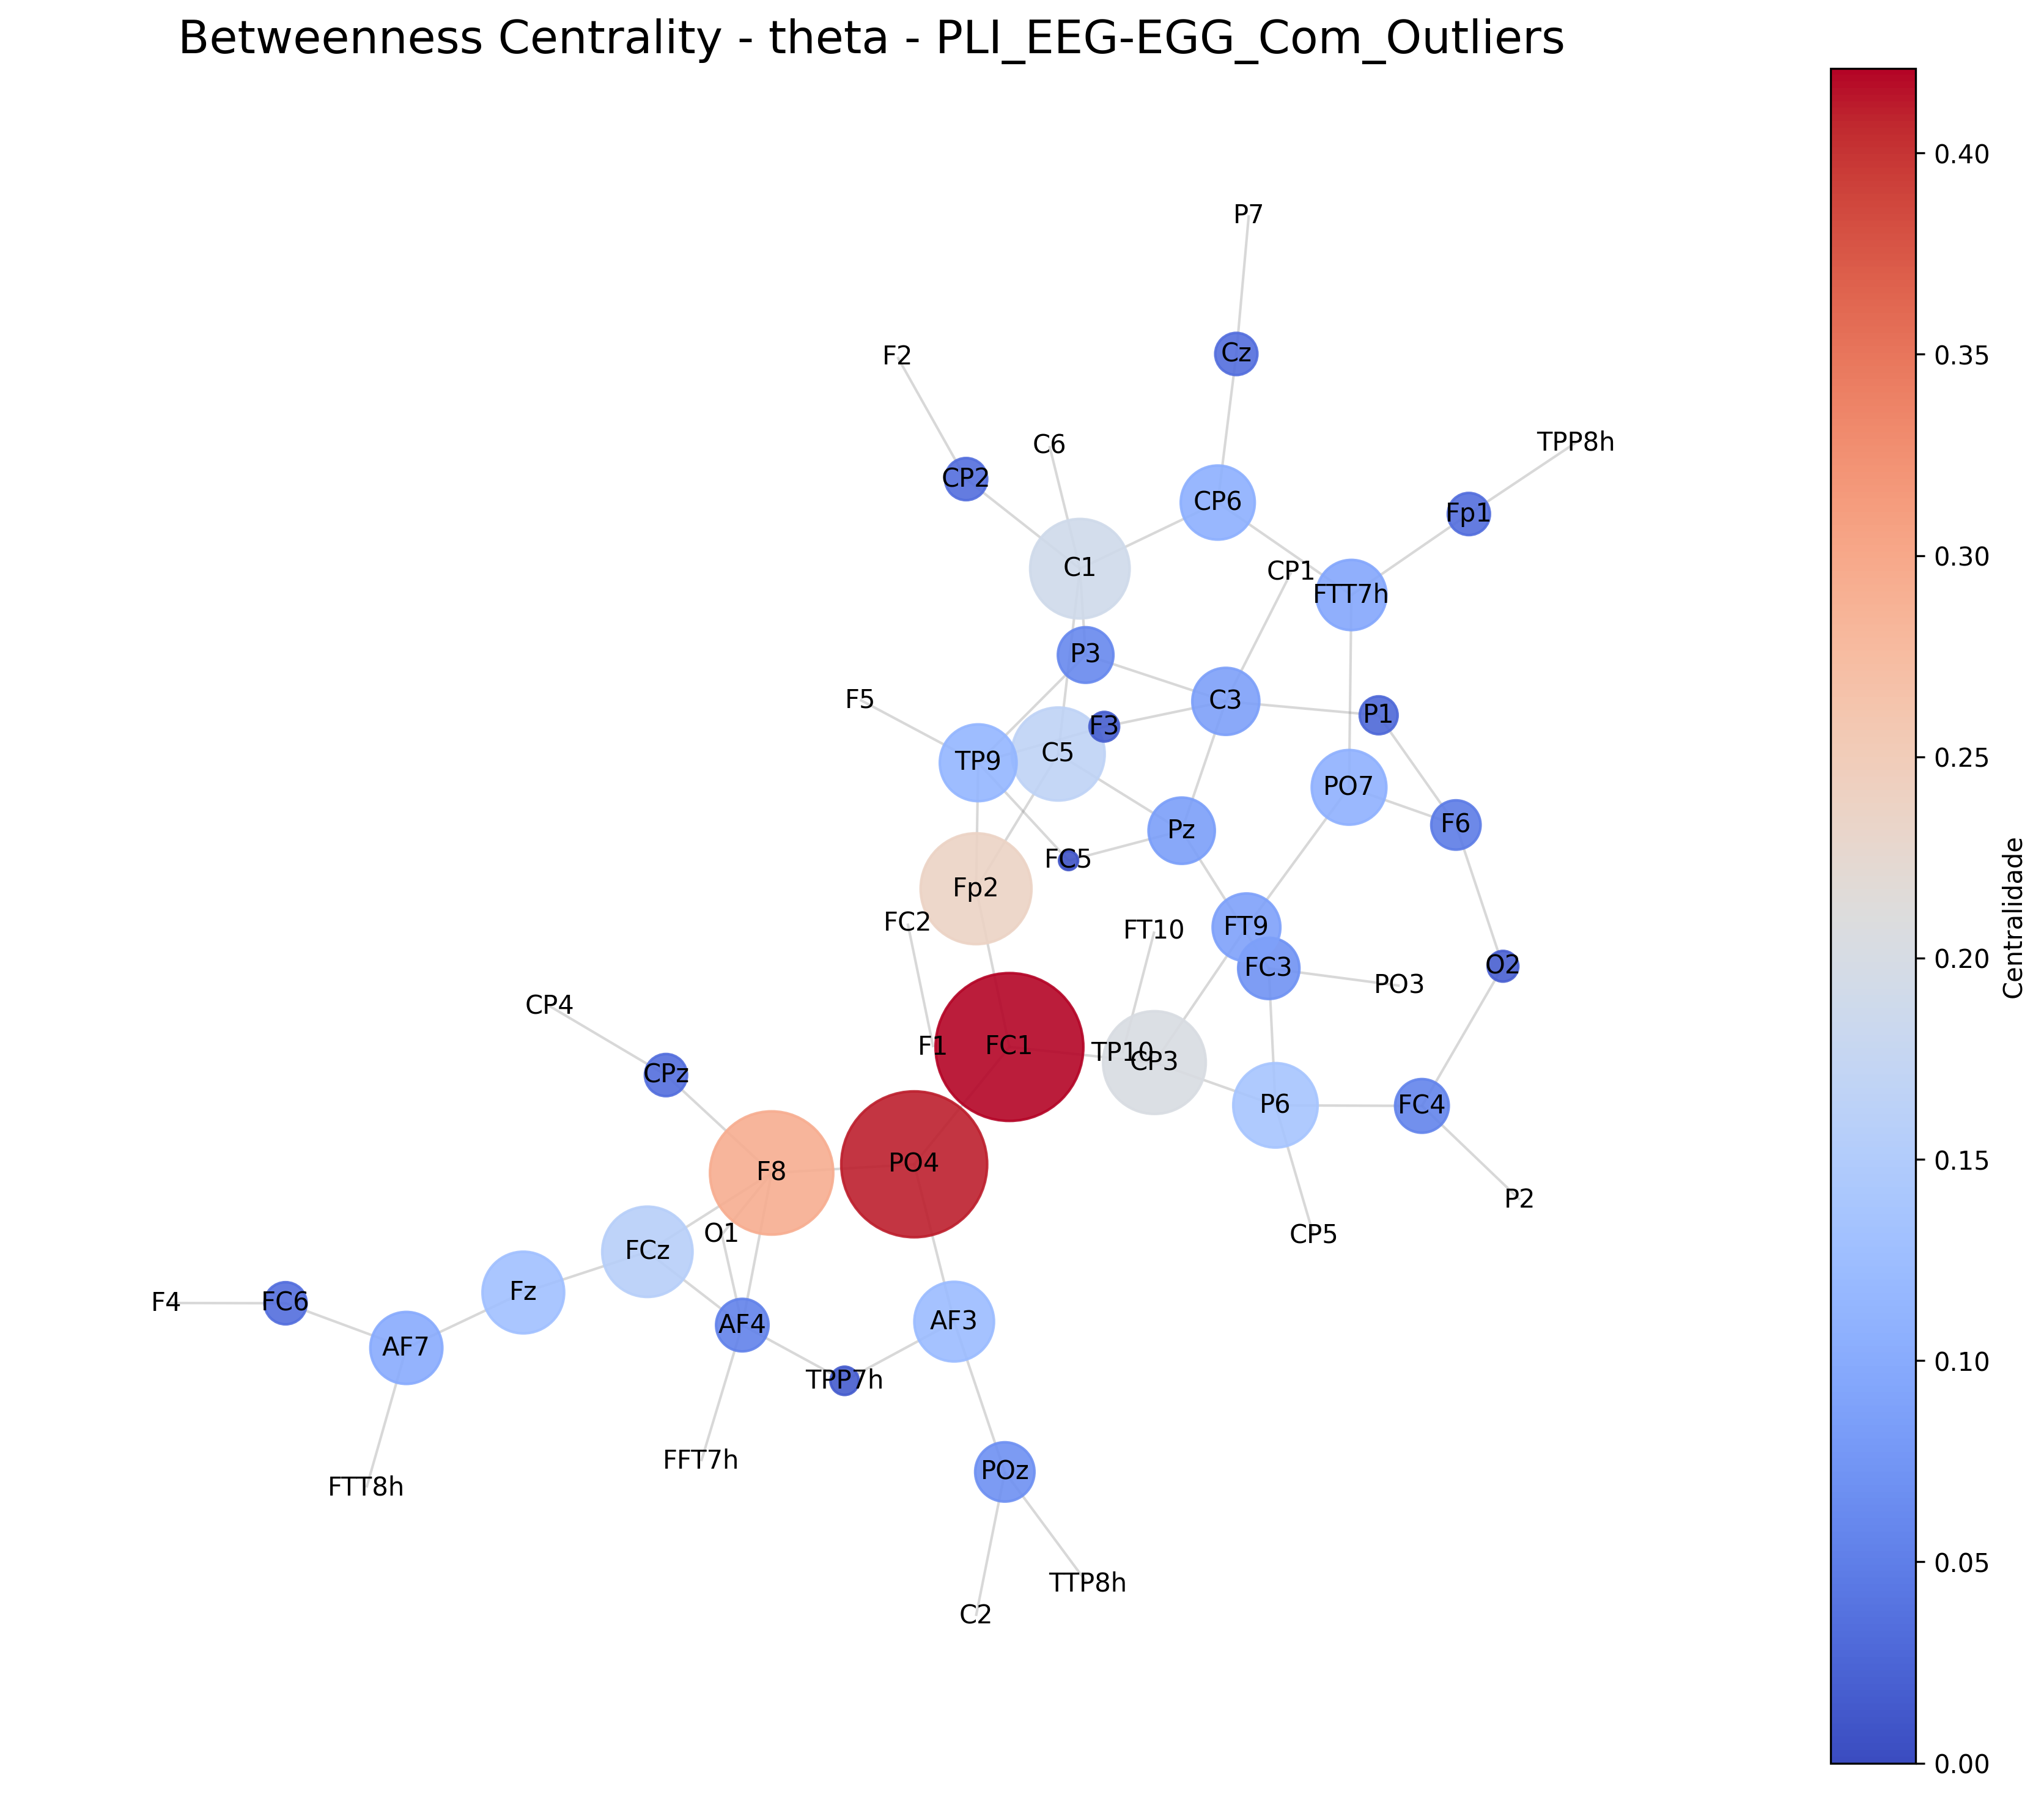
\includegraphics[width=0.45\textwidth]{figs/7_bootstrap_results_analysis/3_centrality_graphs/Com_Outliers/Betweenness_Centrality__theta__PLI_EEGEGG_Com_Outliers.png}
    }
    \hfill
    \subfloat[\small \textbf{Sem Outliers:} Hierarquia – 1. \textbf{PO4}; 2. \textbf{FC1}; 3. \textbf{C5, PO7, P7}; 4. \textbf{F8, AF3, Fp2}.]{%
        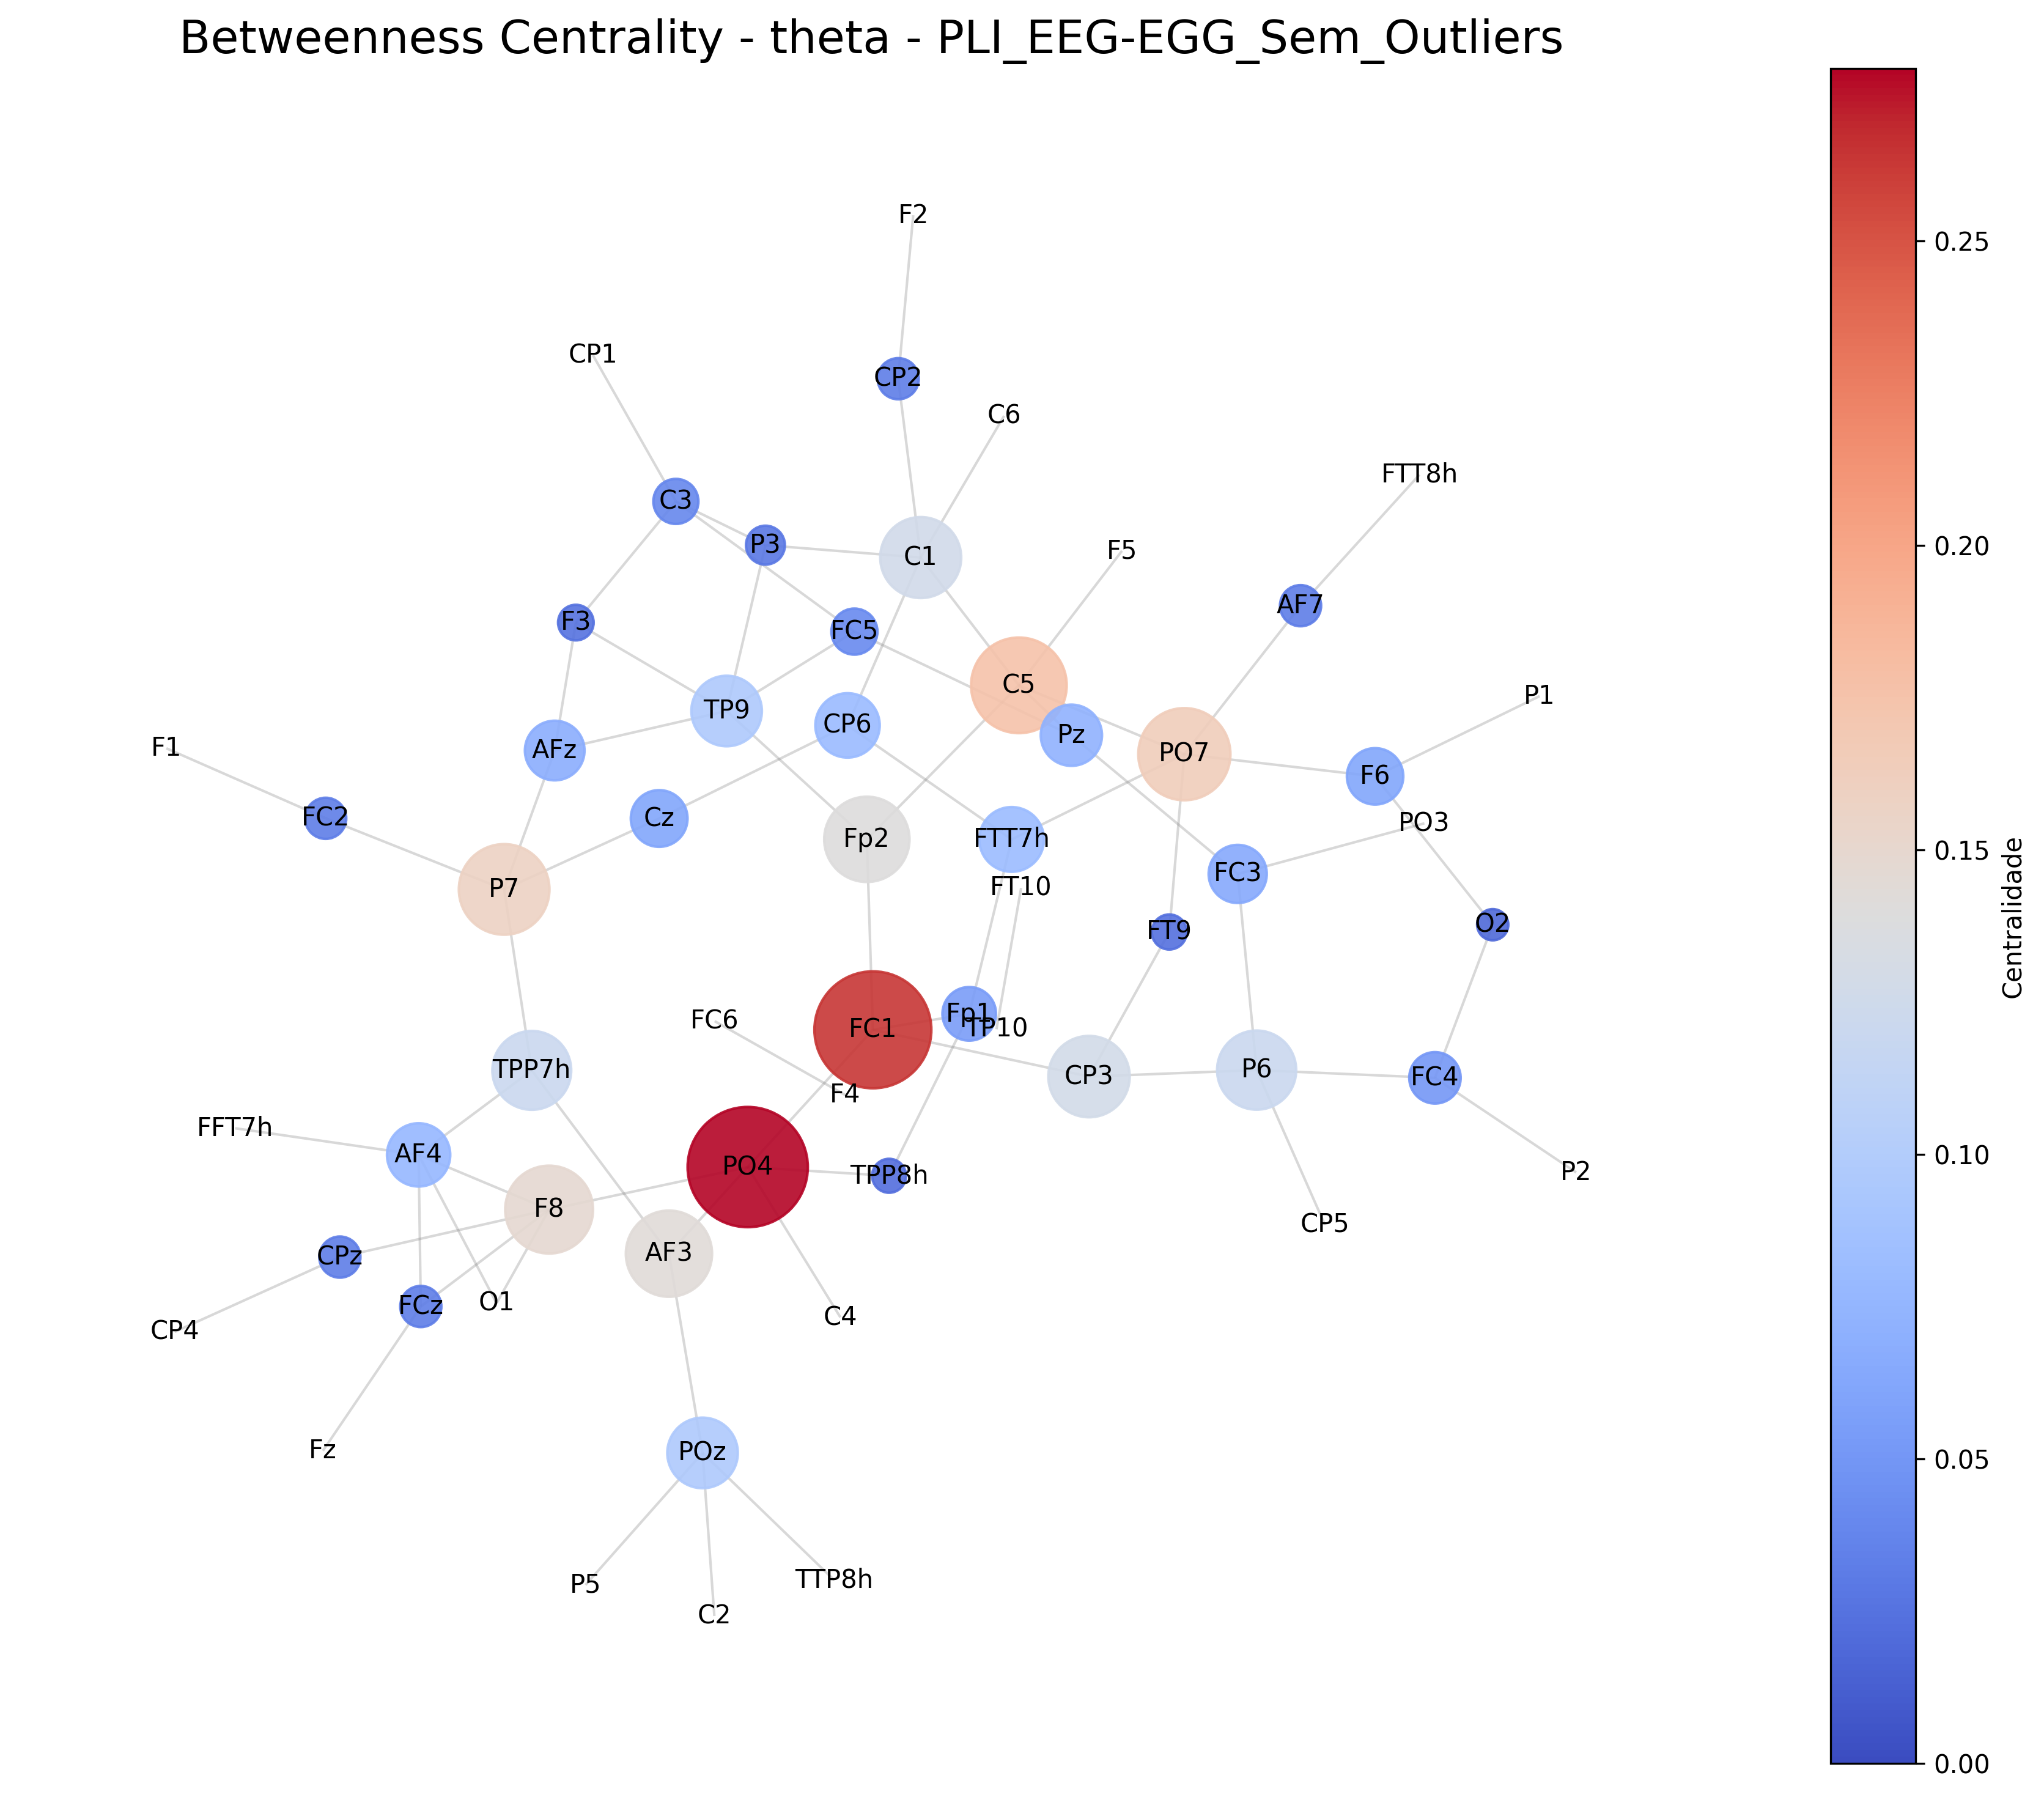
\includegraphics[width=0.45\textwidth]{figs/7_bootstrap_results_analysis/3_centrality_graphs/Sem_Outliers/Betweenness_Centrality__theta__PLI_EEGEGG_Sem_Outliers.png}
    }
    \caption{\small \textbf{Betweenness Centrality – Banda Theta (4--8 Hz):} A rede theta evidencia diferenças sutis na mediação dos caminhos, com reorganização da hierarquia após a remoção dos outliers.}
    \label{fig:betweenness_theta}
\end{figure}

\subsubsection{Degree Centrality}
\begin{figure}[H]
    \centering
    \subfloat[\small \textbf{Com Outliers:} Hierarquia – 1. \textbf{C1, C3, TP9, F8, AF4}; 2. \textbf{Pz, P6}.]{%
        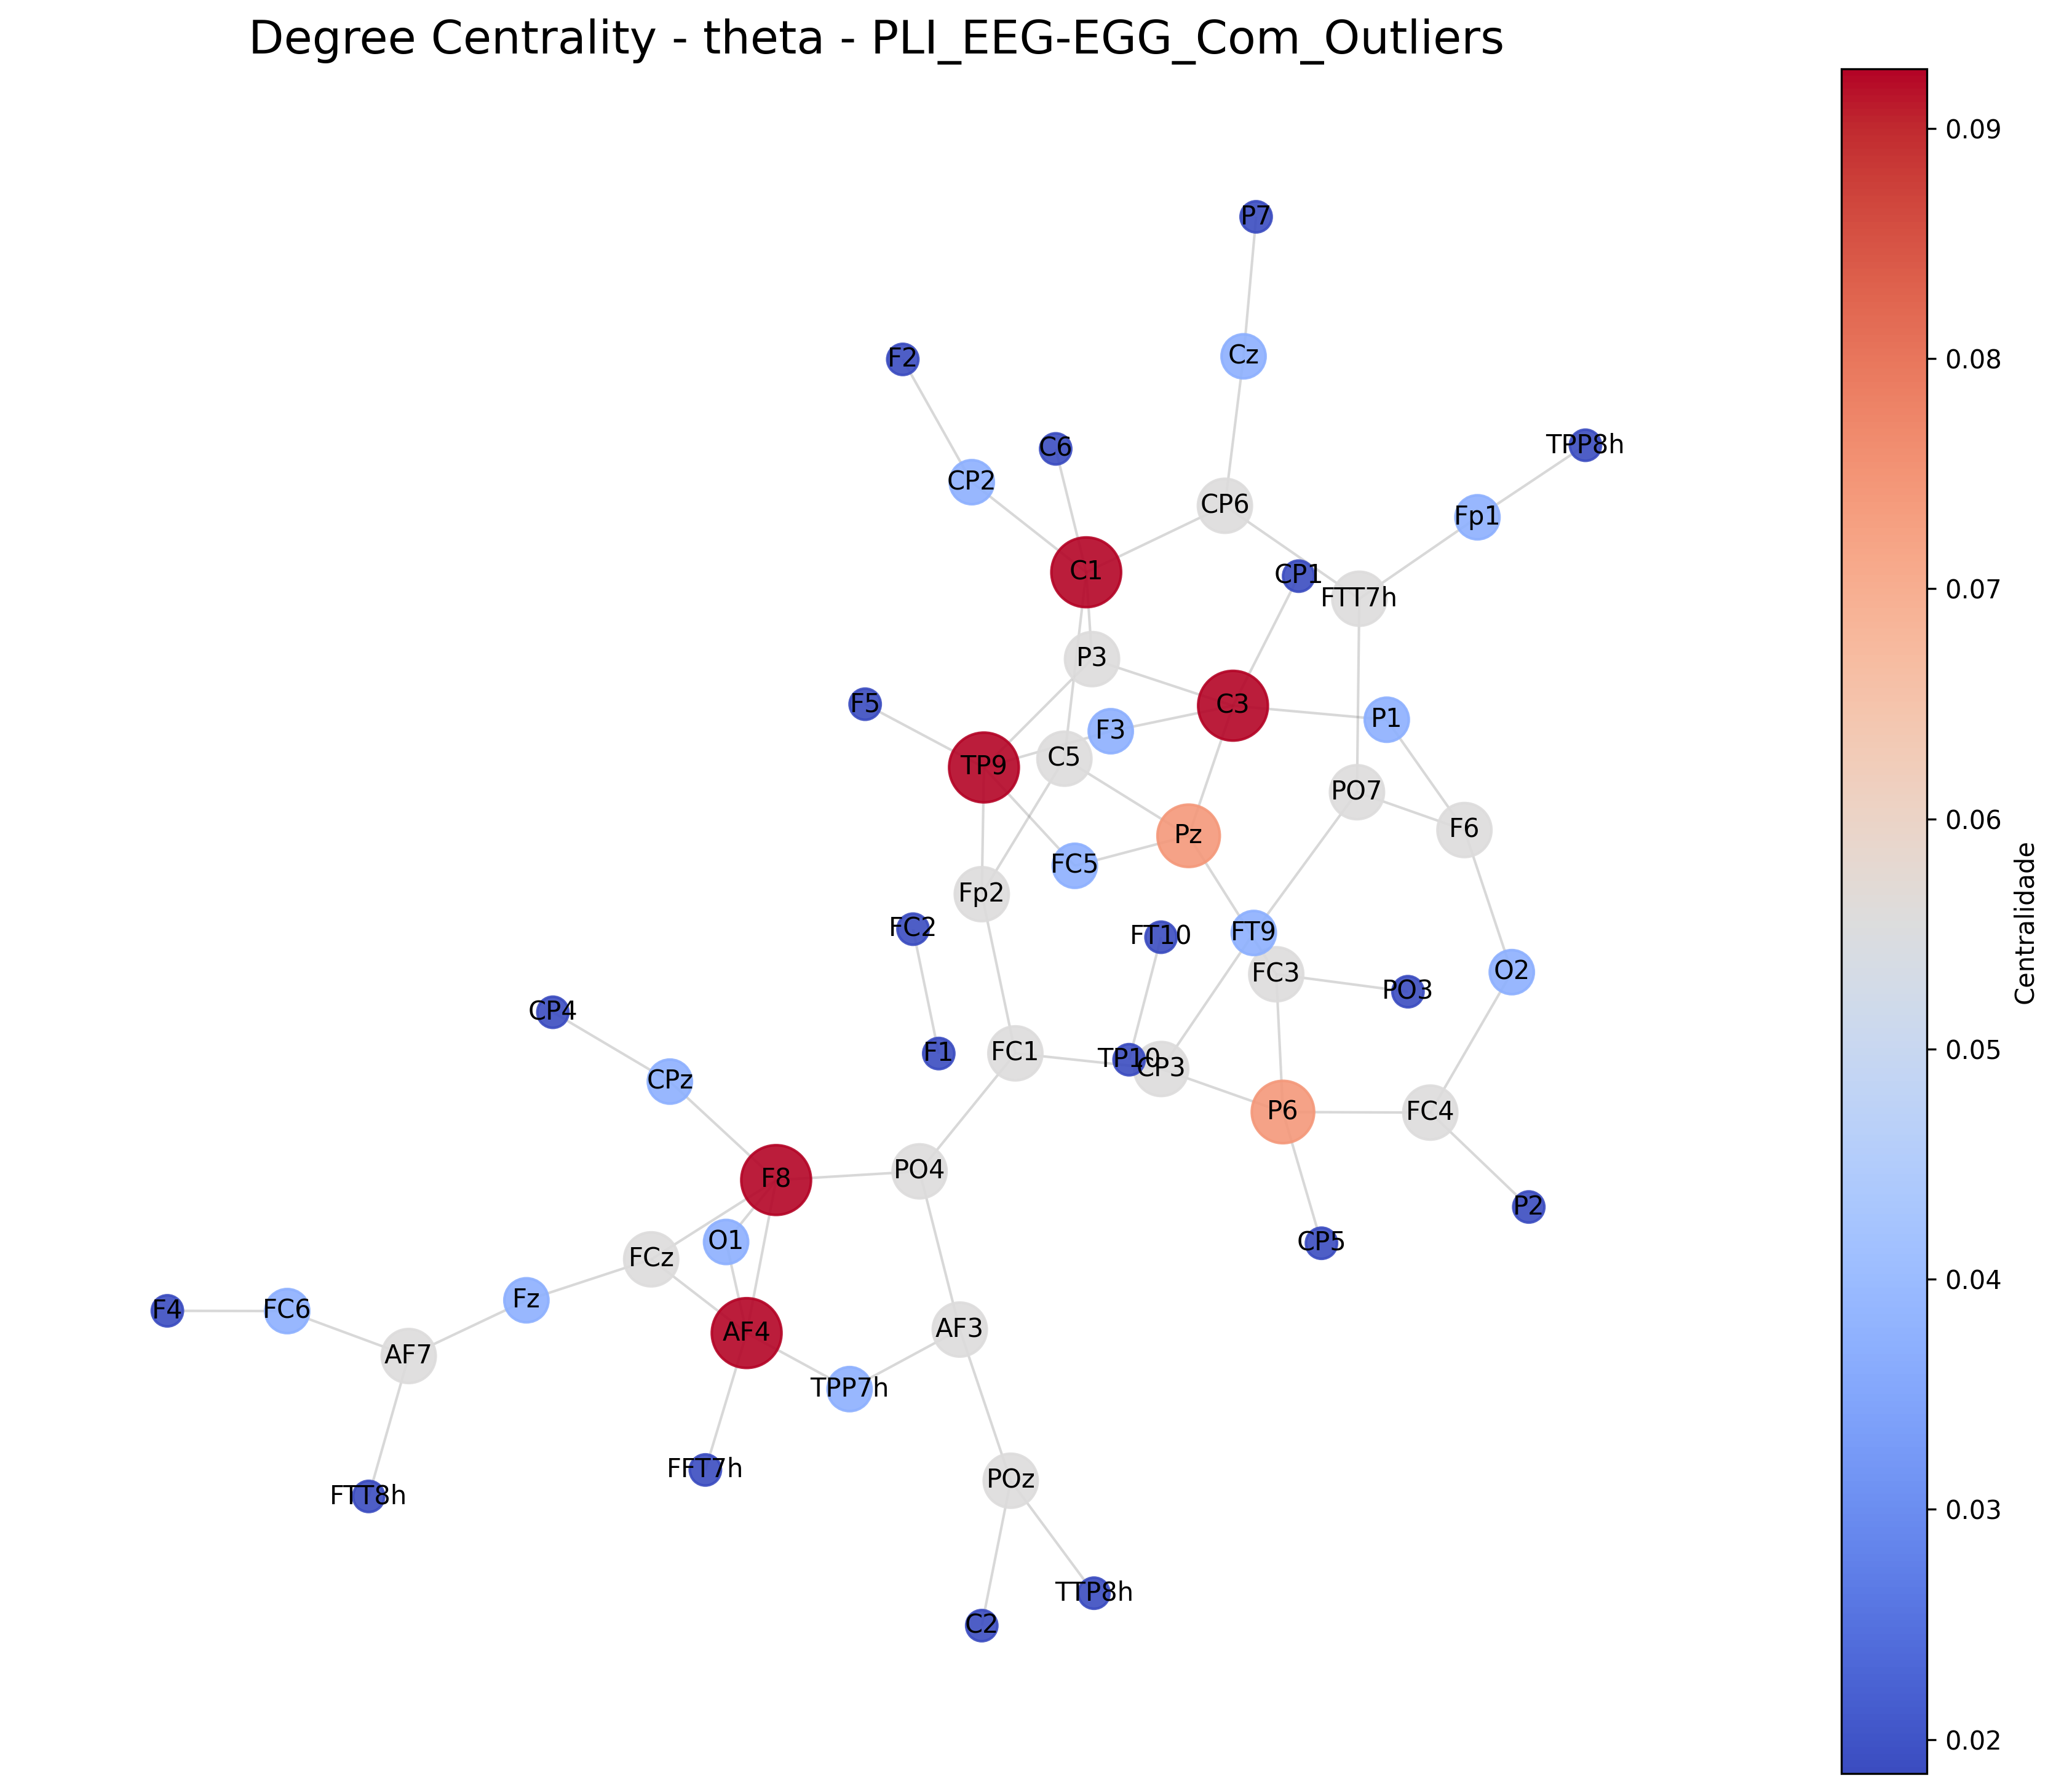
\includegraphics[width=0.45\textwidth]{figs/7_bootstrap_results_analysis/3_centrality_graphs/Com_Outliers/Degree_Centrality__theta__PLI_EEGEGG_Com_Outliers.png}
    }
    \hfill
    \subfloat[\small \textbf{Sem Outliers:} Hierarquia – 1. \textbf{C1, C5, TP9, PO7, PO4, F8, AF4}; 2. \textbf{POz, P7, FC1, P6, C3}.]{%
        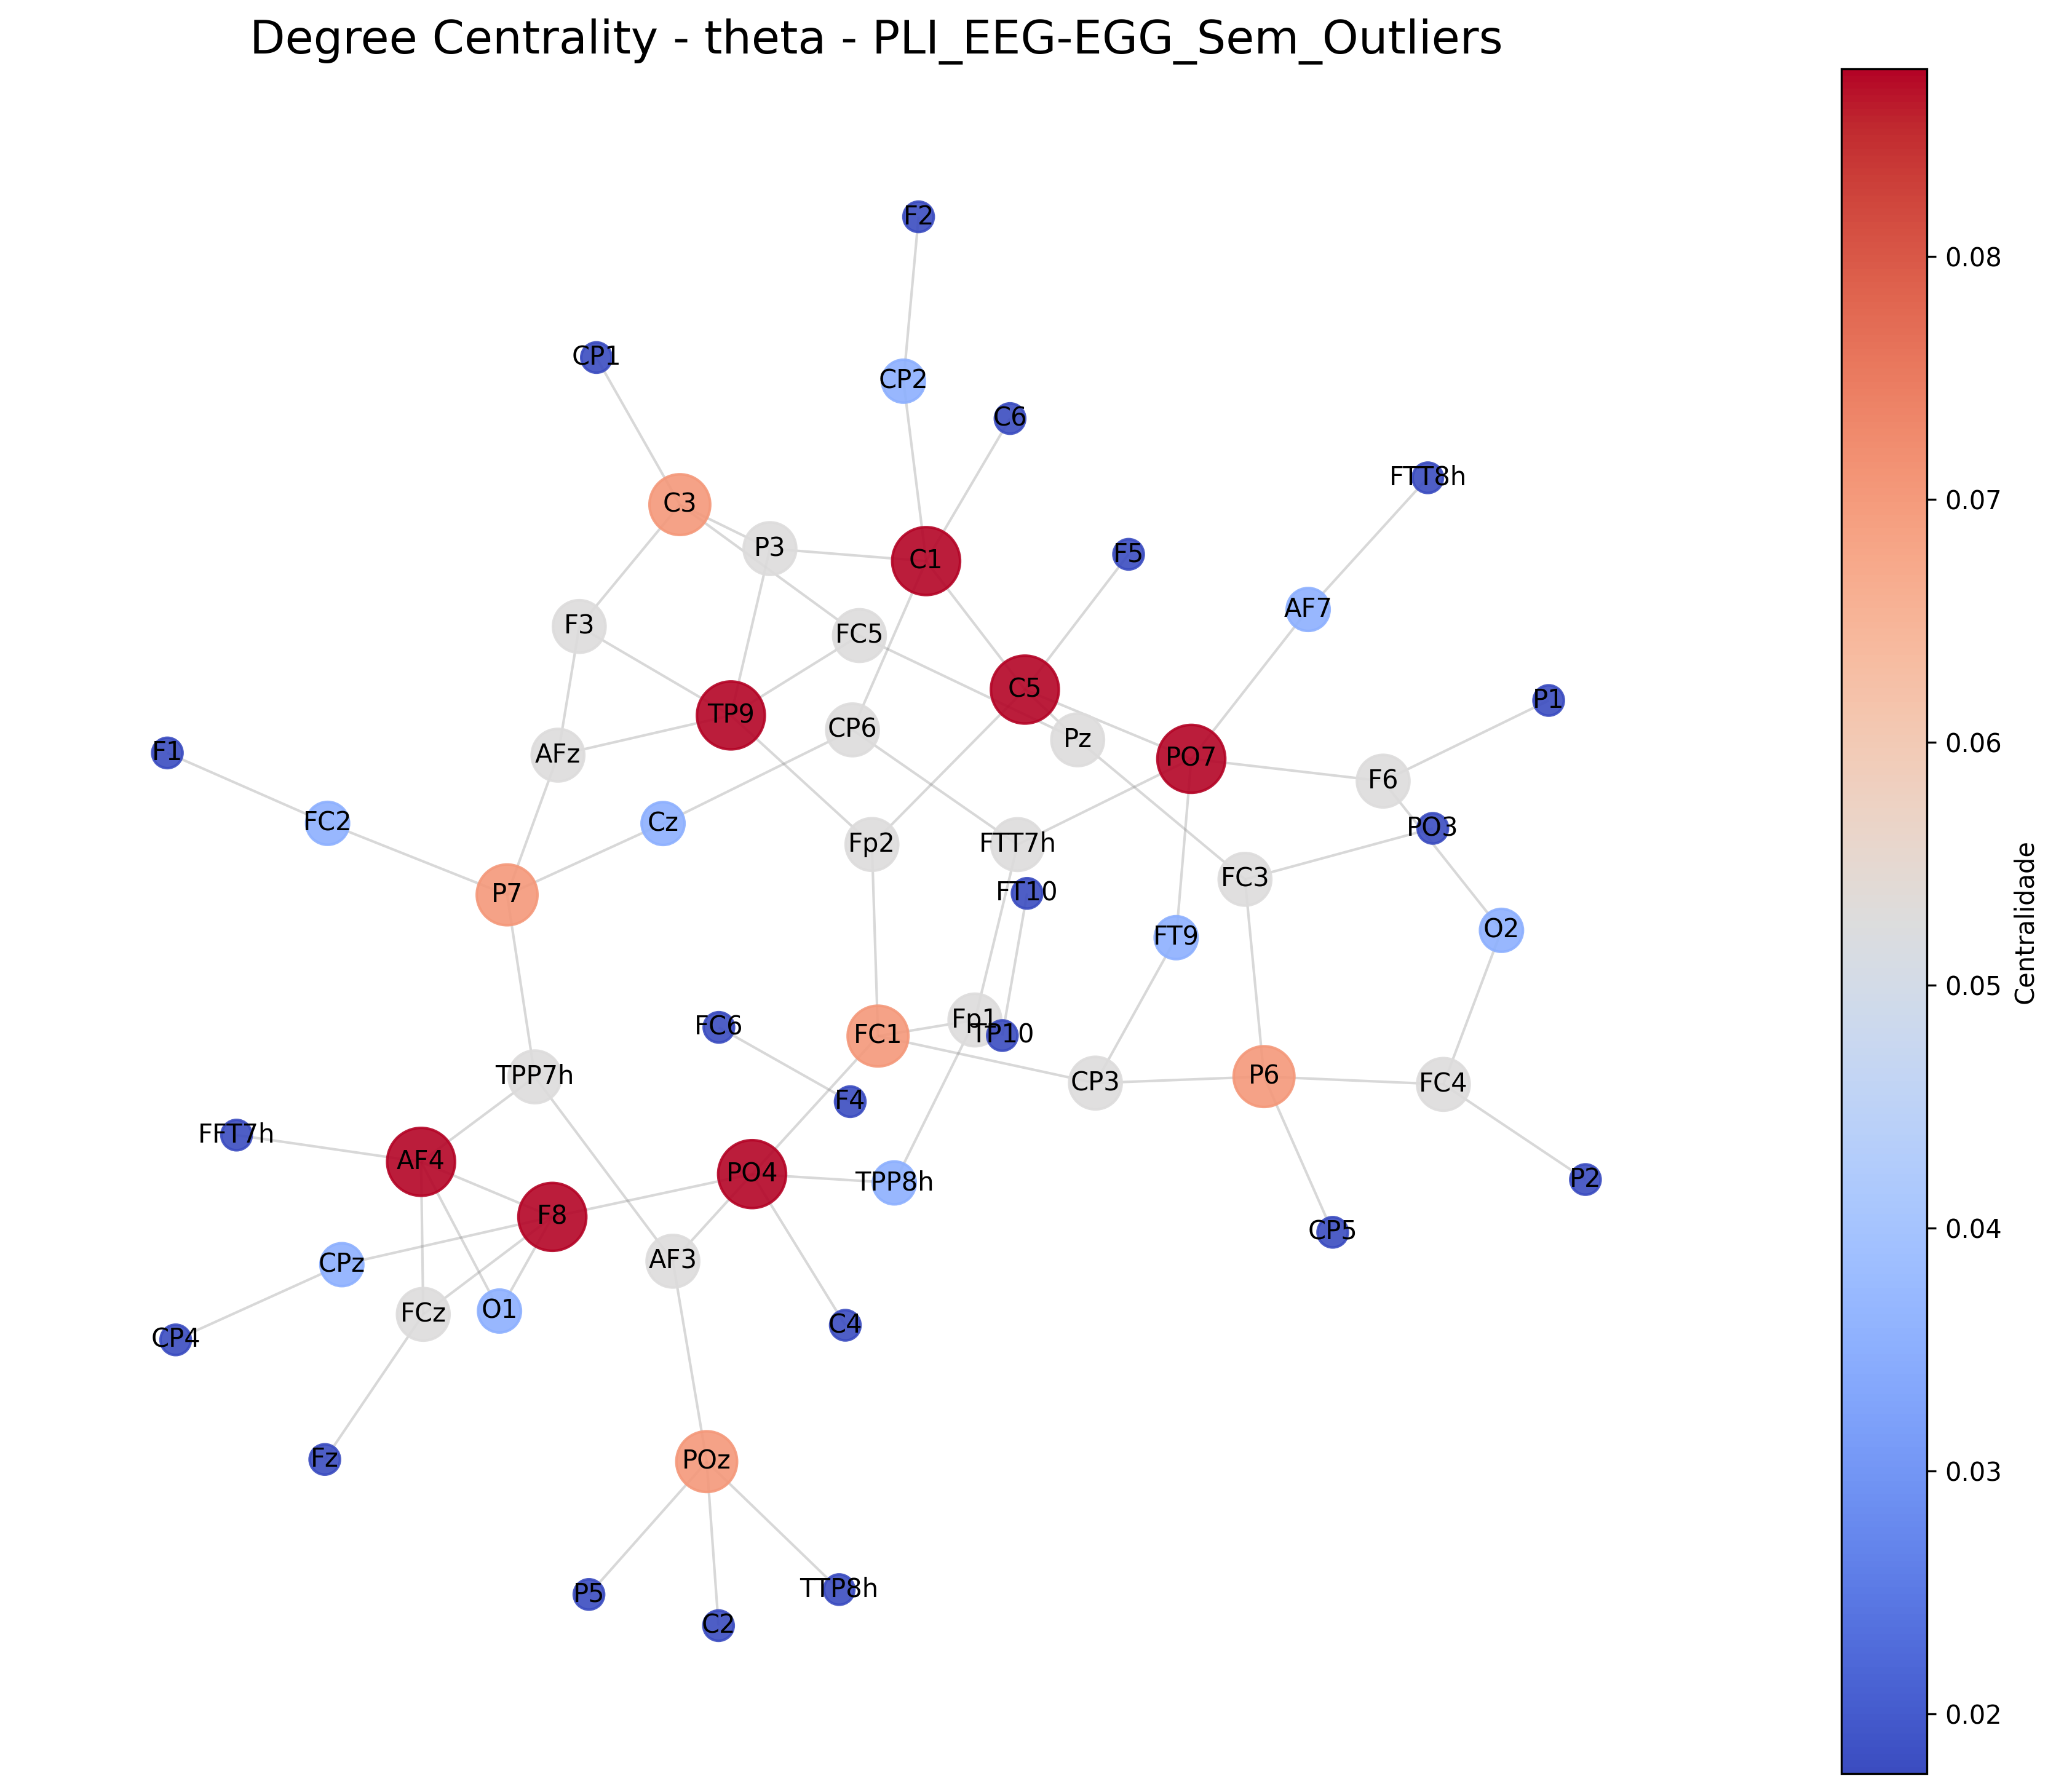
\includegraphics[width=0.45\textwidth]{figs/7_bootstrap_results_analysis/3_centrality_graphs/Sem_Outliers/Degree_Centrality__theta__PLI_EEGEGG_Sem_Outliers.png}
    }
    \caption{\small \textbf{Degree Centrality – Banda Theta (4--8 Hz):} A disposição dos canais na rede theta demonstra uma clara divisão entre nodos de alta e baixa conectividade, com leve reorganização após a remoção de outliers.}
    \label{fig:degree_theta}
\end{figure}

\subsubsection{Eigenvector Centrality}
\begin{figure}[H]
    \centering
    \subfloat[\small \textbf{Com Outliers:} Hierarquia – 1. \textbf{F8}; 2. \textbf{AF4}; 3. \textbf{FCz}; 4. \textbf{O1}; 5. \textbf{PO4, TP9}.]{%
        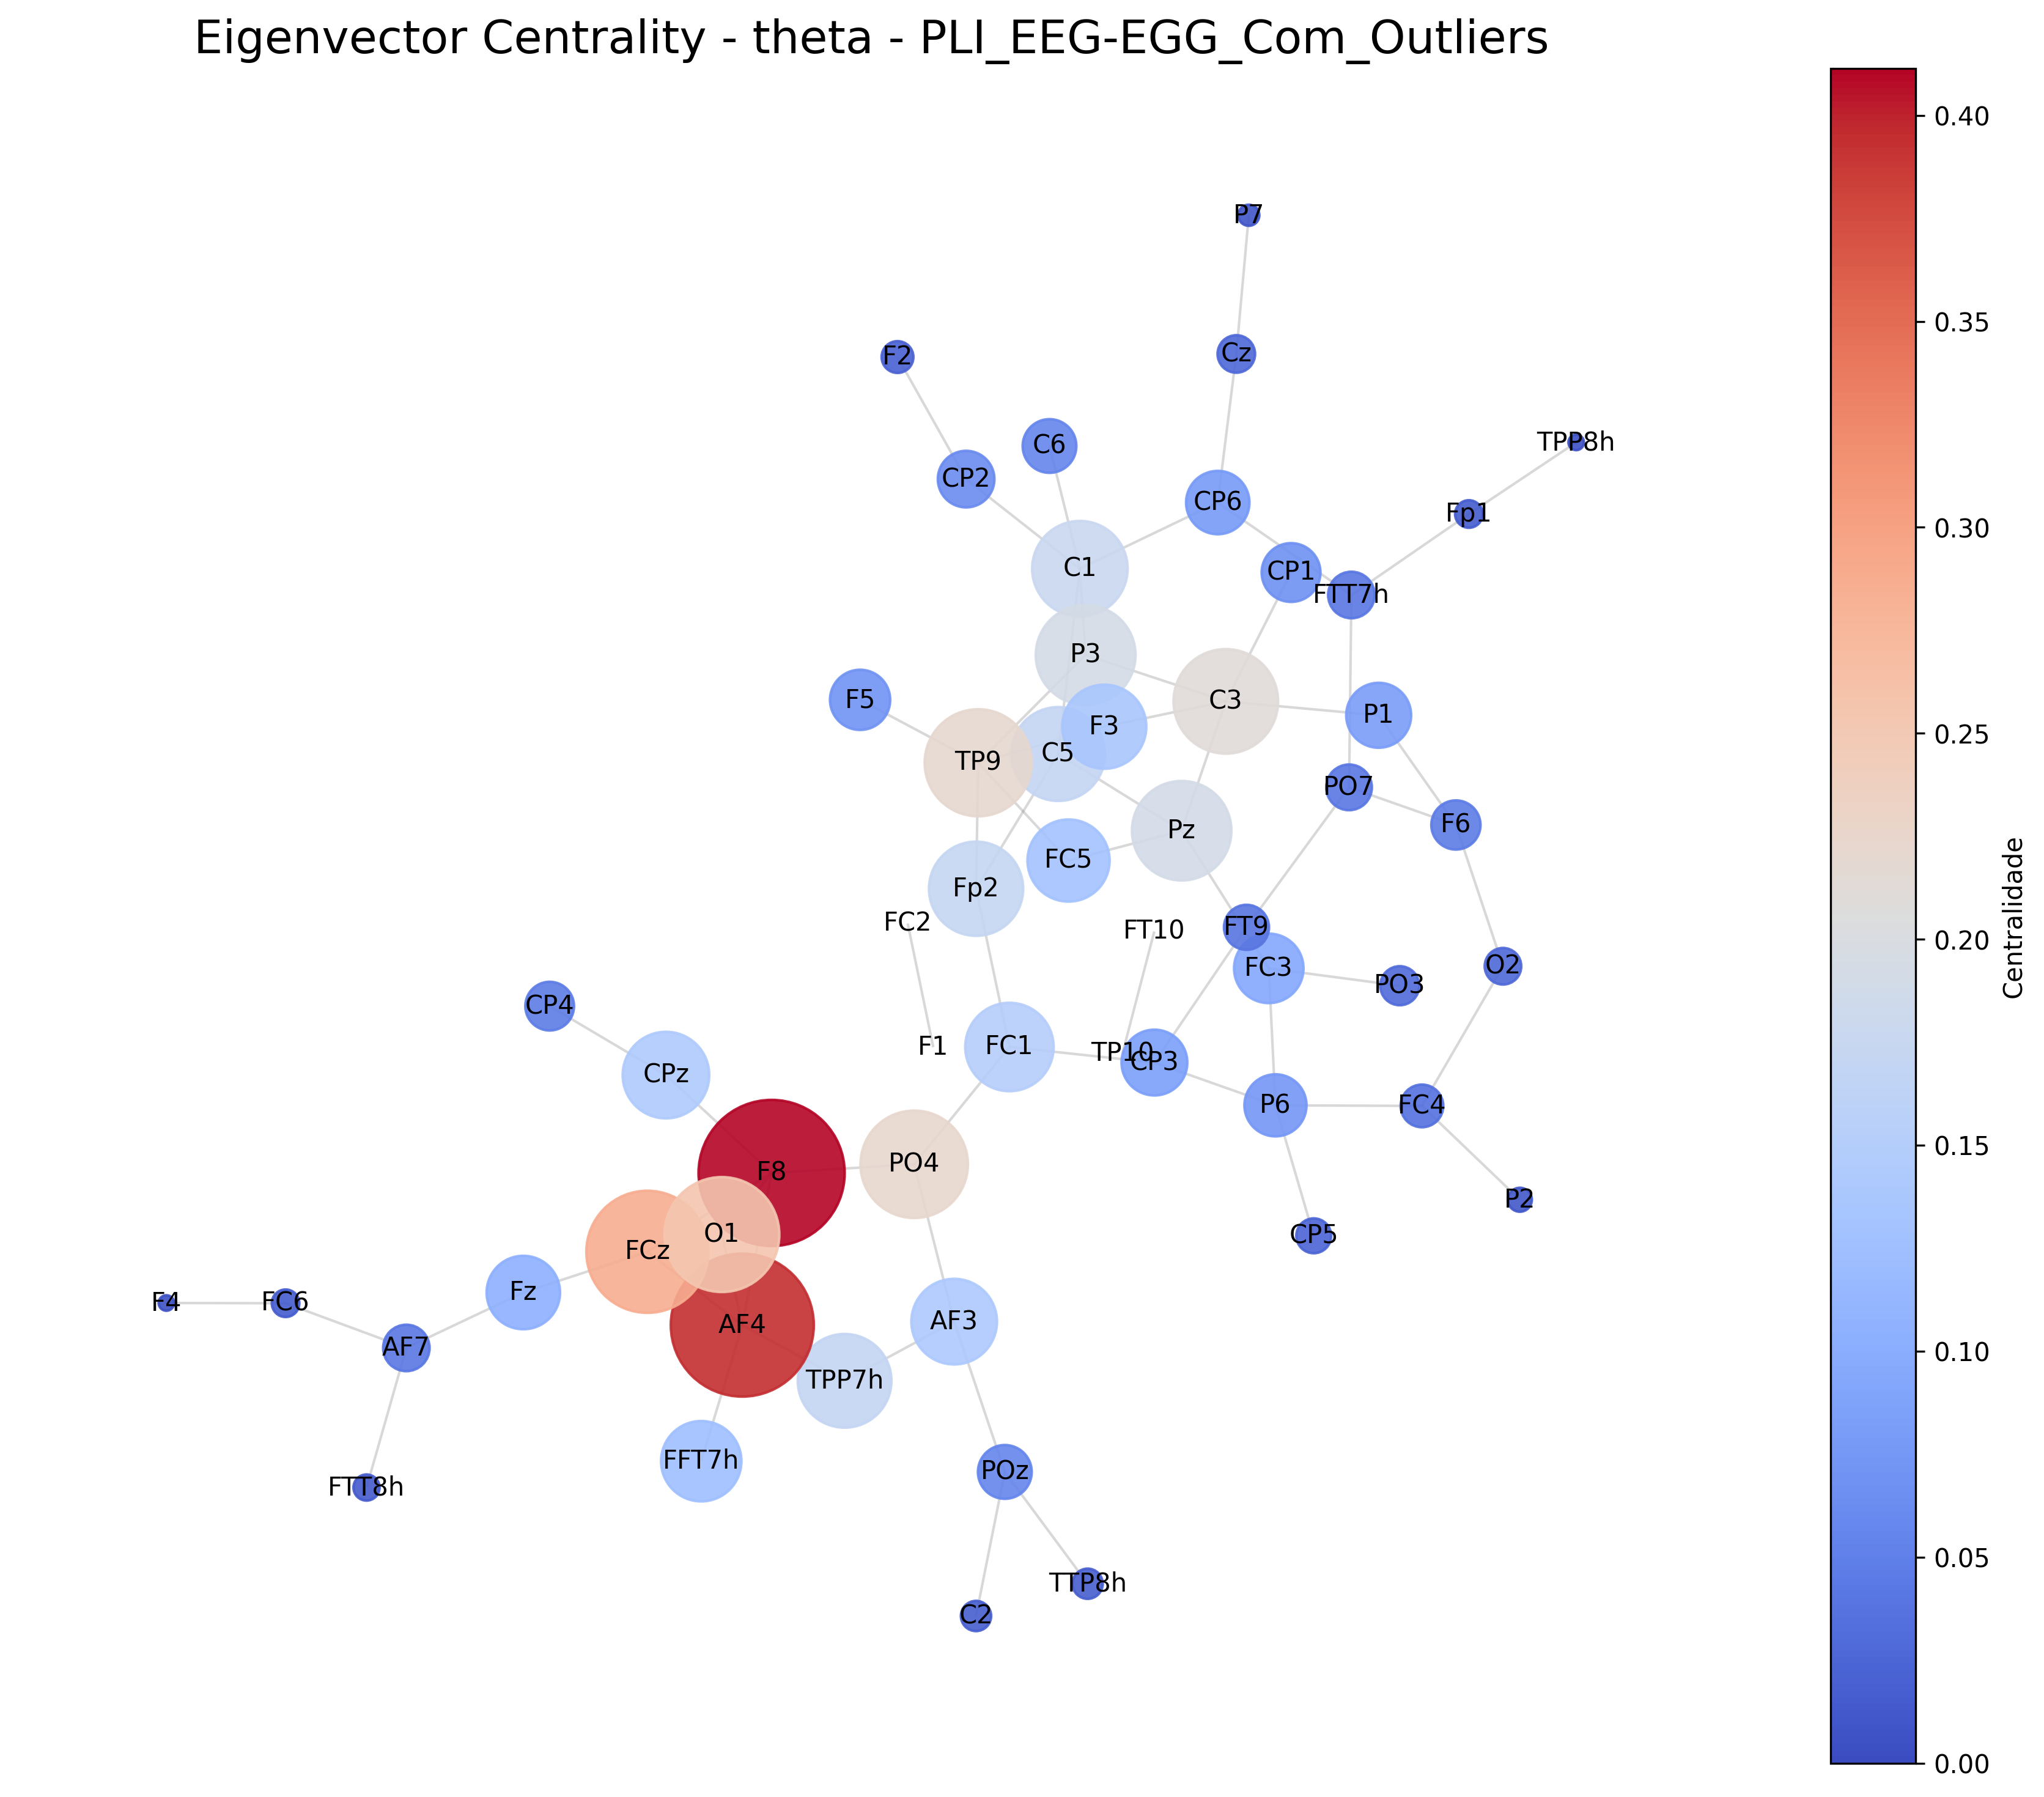
\includegraphics[width=0.45\textwidth]{figs/7_bootstrap_results_analysis/3_centrality_graphs/Com_Outliers/Eigenvector_Centrality__theta__PLI_EEGEGG_Com_Outliers.png}
    }
    \hfill
    \subfloat[\small \textbf{Sem Outliers:} Hierarquia – 1. \textbf{TP9}; 2. \textbf{C5}; 3. \textbf{Fp2, C1, P3, F3, F8, FC5, FC1, C3, AFz, AF4, PO4, FC1}.]{%
        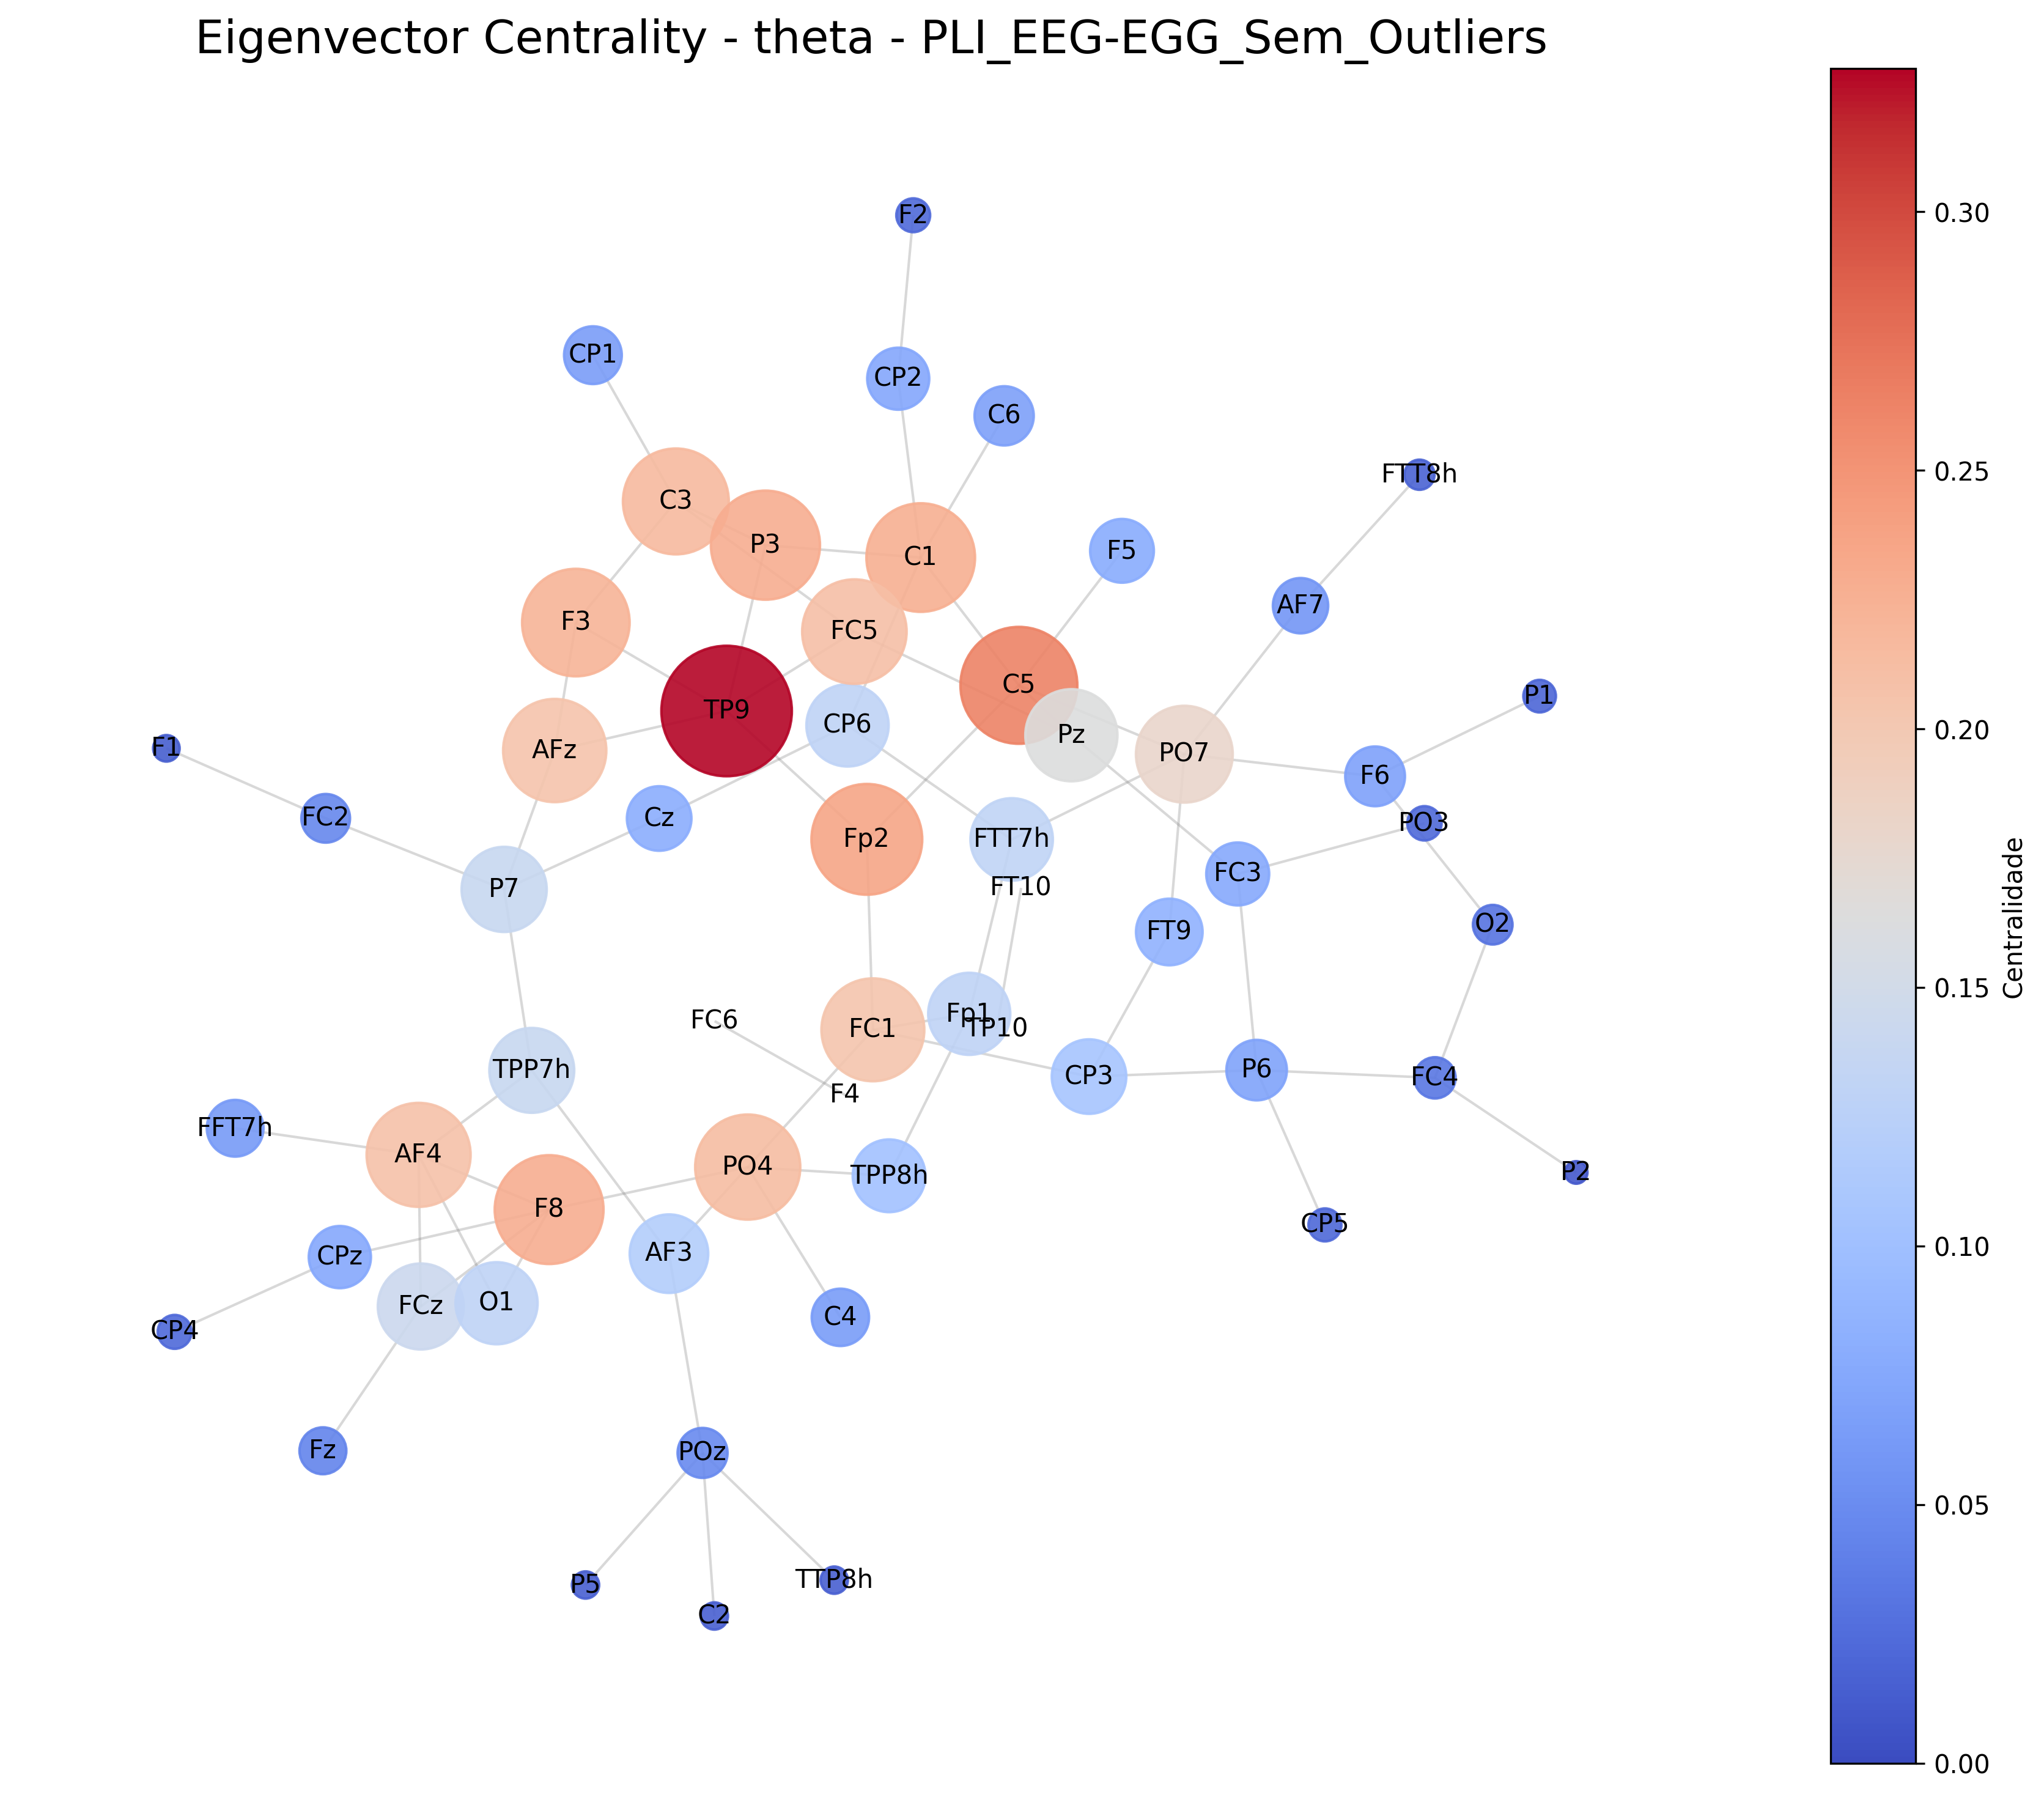
\includegraphics[width=0.45\textwidth]{figs/7_bootstrap_results_analysis/3_centrality_graphs/Sem_Outliers/Eigenvector_Centrality__theta__PLI_EEGEGG_Sem_Outliers.png}
    }
    \caption{\small \textbf{Eigenvector Centrality – Banda Theta (4--8 Hz):} As figuras evidenciam a hierarquia de influência na rede theta, com reorganização mais evidente na versão sem outliers.}
    \label{fig:eigenvector_theta}
\end{figure}

\section{Considerações Finais sobre a Centralidade de Grafos}
Os gráficos de centralidade apresentados evidenciam a hierarquia dos canais na rede de conectividade EEG–EEG (obtida via PLI). Em todas as métricas, os nós com maior centralidade – indicados por cores mais intensas (vermelho) e maiores tamanhos – correspondem a canais que atuam como hubs ou pontos-chave na rede. 

Observa-se que:
\begin{itemize}
    \item \textbf{Exibição dos Dados:} Apenas os casos de PLI EEG–EEG foram apresentados, uma vez que a análise de CF‐PLM (EEG–ECG) não fornece uma hierarquia diferenciada entre canais, dado que o ECG aparece em todas as conexões.
    \item \textbf{Hierarquia e Distribuição:} Em cada banda, os canais mais relevantes são listados em ordem decrescente de centralidade. Por exemplo, na banda Alpha, o canal \textbf{Fp2} é consistentemente o mais central, seguido por grupos de canais como \textbf{PO8}, \textbf{FC3} e outros, com pequenas variações entre os cenários com e sem outliers. Em bandas como Beta e Gamma, determinados canais (por exemplo, \textbf{TPP7h} na banda Beta e \textbf{FT10} na banda Gamma) se destacam como hubs principais.
    \item \textbf{Impacto da Remoção de Outliers:} Embora a remoção de outliers gere ajustes nos valores absolutos de centralidade e, consequentemente, na ordem intermediária dos canais, a estrutura global da rede se mantém similar entre os cenários. Em alguns casos, a hierarquia se reorganiza, como na banda Delta, onde a remoção de outliers desloca a centralidade de canais frontais (como \textbf{Fp2}) para canais parietais (\textbf{CP5} e \textbf{CP4}).
    \item \textbf{Padrões entre Bandas:} As bandas Alpha e Theta tendem a apresentar elevados valores de centralidade, refletindo uma maior integração e influência dos nós nessas frequências. Em contraste, a banda Delta exibe uma hierarquia mais sensível à presença de outliers, enquanto nas bandas Beta e Gamma certos canais se destacam de forma consistente.
\end{itemize}

Essas observações contribuem para a compreensão dos efeitos da neuromodulação na dinâmica da conectividade neural, destacando a importância dos canais em diferentes bandas de frequência e demonstrando a robustez dos achados mesmo após a remoção de outliers.

\chapter{Resultados e Discussões}
\label{chap:resultados_e_discussoes}

A compreensão dos mecanismos neurobiológicos subjacentes aos efeitos da neuromodulação não-invasiva é uma das fronteiras atuais da neurociência aplicada ao esporte de alto rendimento. Neste capítulo, integramos os resultados obtidos com a estimulação transcraniana por corrente contínua de alta definição (HD-tDCS) catódica aplicada ao córtex pré-frontal dorsolateral (DLPFC) esquerdo, discutindo-os em quatro eixos complementares:

\begin{enumerate}
  \item \textbf{Sincronização de fase intrafrequencial} (\emph{EEG-EEG}) quantificada pelo \textit{Phase Lag Index} (PLI);
  \item \textbf{Acoplamento \textit{cross-frequency}} (\emph{EEG-ECG}) mensurado pelo \textit{Cross-Frequency Phase Linearity Measurement} (CF-PLM);
  \item \textbf{Significância estatística e magnitude dos efeitos} - primeiro por testes não-paramétricos globais (Mann-Whitney U, Wilcoxon signed-rank e Kruskal-Wallis) e, em seguida, por estimativas \emph{bootstrap} par-a-par (Hedges' g e \textit{Rank-Biserial Correlation});
  \item \textbf{Organização topológica do efeito da neuromodulação} avaliada por métricas de teoria de grafos e centralidade.
\end{enumerate}

Esses domínios metodológicos são detalhados nos Capítulos~\ref{chap:6_metodos_de_analise_de_sincronizacao_de_fase}-\ref{chap:analise_centralidade_de_grafos}. A seguir apresentamos os achados, distinguindo a fase \emph{macro} (testes globais sobre o conjunto completo de amostras) da fase \emph{micro} (\emph{bootstrap} par-a-par, cujas análises gráficas estão nos Capítulos \ref{chap:analise_de_rede} e \ref{chap:analise_centralidade_de_grafos}, e os dados completos estão no repositório público\footnote{\url{https://github.com/dantebarross/efeito-da-neuromodulacao-na-sincronicidade-eeg-ecg}}).

%-------------------------------------------------------------------
\section{Análise de Sincronização de Fase}
%-------------------------------------------------------------------

\subsection{Conectividade intrafrequencial (\emph{EEG-EEG})}

Os testes globais (Mann-Whitney U/Kruskal-Wallis) apontaram:
\begin{itemize}
  \item alpha, delta, theta e gamma: $p<\alpha_{\mathrm{corr}}=\mathbf{0{,}005}$;
  \item beta: efeito marginalmente não-significativo ($p=0{,}052$).
\end{itemize}

\inputtable{tabelas/nonparametric_tests_results.tex}
{Resultados dos testes não-paramétricos (Mann-Whitney U, Wilcoxon signed-rank e Kruskal-Wallis) por faixa de frequência e grupo de canais}
{tab:nonparametric_results}
{Elaborado pelo autor (2025). Nota: * indica significância estatística ($p < \alpha_{\mathrm{corr}}$).}

Em todas as faixas em que houve significância global (alpha, delta, theta, gamma), a análise \emph{bootstrap} confirmou robustez do sinal e permitiu estimar:
\begin{itemize}
  \item \textbf{Alpha:} aumento da diferença Pós–Pré sob catódica (RBC médio $\approx+1$);
  \item \textbf{Delta \& Gamma:} diminuição da sincronia sob catódica (RBC médio $\approx-1$).
\end{itemize}

%-------------------------------------------------------------------
\subsection{Acoplamento \emph{cross‐frequency} (\emph{EEG–ECG})}
%-------------------------------------------------------------------

Nos testes globais, apenas beta e delta atingiram $p<0{,}005$ (gamma marginalmente não-significativo, $p\approx0{,}00505$); alpha e theta ficaram fora do limiar.

A fase \emph{micro} (\emph{bootstrap}) confirmou:
\begin{itemize}
  \item \textbf{Beta e Delta:} redução consistente do acoplamento catódica \textit{versus} sham (RBC médio $\approx+0.9$);
  \item \textbf{Gamma:} redução moderada (RBC $\approx+1$).
\end{itemize}

%-------------------------------------------------------------------
\subsection{Pipeline Estatístico}
%-------------------------------------------------------------------

\subsubsection{Fase 1 - Testes Globais} 
Aplicamos Mann-Whitney U e Kruskal-Wallis para amostras independentes e Wilcoxon signed-rank para amostras pareadas, com correção de Bonferroni em função dos 10 testes totais (2 grupos × 5 bandas) ($\alpha_{\mathrm{corr}}=0{,}005$). Resultados completos na Tabela \ref{tab:nonparametric_results}. Aqui está a síntese dos resultados globais:
\begin{itemize}
    \item A HD-tDCS catódica \emph{potenciou} significativamente a sincronia alpha em EEG-EEG e \emph{reduziu} sincronia em delta/gamma.
    \item Em EEG-ECG, houve \emph{redução} de acoplamento em beta, delta e gamma.
    \item Os testes globais e o \textit{bootstrap} convergiram nas direções e magnitudes de efeito (RBC próximos a \(\pm1\)).
  \end{itemize}

\subsubsection{Fase 2 - \textit{Bootstrap} Par-a-Par} 
Nessa etapa, para cada par de canais realizamos 10.000 reamostragens (\textit{bootstrap}) BCa aceleradas por GPU, a partir das quais extraímos a diferença média Pós–Pré (\(\bar{\Delta}\)), o \textit{bias} da estimativa, o erro-padrão (\(\mathrm{SE}\)) e o intervalo de confiança BCa a 95\%. Além disso, calculamos a estatística de Wilcoxon (\(W\)) e sua correlação bisserial de postos (RBC), o tamanho de efeito de Hedges' \(g\) corrigido para amostras pequenas, o p-valor empírico em duas faces gerado pelo bootstrap. Utilizamos Bonferroni, Holm e FDR-BH como métodos de correção; para as análises de redes e medidas de centralidade, adotamos Bonferroni. Os resultados par-a-par completos (54.900 pares EEG-EEG e 1.830 pares EEG-ECG) estão no repositório.

\section{Discussão Integrada}
% --- síntese entre intrafreq e cross-freq ---
Em ambas as análises, intrafrequencial (PLI) e \textit{cross-frequency} (CF-PLM), o ritmo alpha emergiu como o mais sensível à HD-tDCS catódica, tanto estatisticamente quanto em tamanho de efeito. Já a banda beta mostrou um padrão heterogêneo, com significância marginal nos testes globais mas efeitos moderados em pares selecionados. Essa dissociação reforça a ideia de que diferentes circuitos e escalas de acoplamento (local \textit{versus} corpo-coração) respondem de maneira distinta à neuromodulação, possivelmente por diferenças em sua arquitetura anatômica e fisiologia de geração de oscilação.

% --- implicações de rede e hubs ---
Na construção da rede, cada aresta reflete o quanto a estimulação catódica alterou a sincronia em relação ao sham (diferença cathodic-sham) após 10.000 reamostragens BCa e correção de Bonferroni. Ou seja, não se trata de uma rede da sincronia basal em repouso, mas de uma rede das mudanças induzidas pela HD-tDCS.

Nas medidas de centralidade, os canais de maior centralidade correspondem, portanto, àqueles que participaram de um maior número de pares em que o efeito da HD-tDCS sobre a sincronia foi mais pronunciado. Na banda \textbf{alpha} (8-13 Hz), o canal \textbf{Fp2} emergiu como hub de maior centralidade em todas as métricas (\textit{Betweenness}, \textit{Degree} e \textit{Eigenvector}), tanto com outliers quanto sem outliers, indicando que é justamente nessa região que as ocorrências de pares com maiores diferenças cathodic-sham foram mais frequentes.

Em outras faixas de frequência, observamos reorganizações na hierarquia de \textit{hubs}: por exemplo, \textbf{TPP7h} na banda \textbf{beta} e, no cenário sem remoção de outliers, \textbf{CP5} e \textbf{CP4} na banda \textbf{delta}.

% --- link com a literatura ---
Esses achados corroboram o conceito de que a HD-tDCS induz mudanças agudas e persistentes na sincronização cortical (ou seja, uma forma de plasticidade funcional induzida pela corrente contínua) conforme demonstrado por \citeonline{kunze2014high}, e o conceito de ``integração corpo-cérebro'' de \citeonline{criscuolo2022cognition}, ampliando-os ao contexto de atletas de elite em \emph{resting-state}.

% --- brainstorming quanto ao futuro ---
Futuros estudos poderão investigar se esses \emph{hubs} de modulação de sincronia, especialmente o reforço da sincronização alpha em Fp2 e o aumento do acoplamento cérebro-coração, traduzem-se em ganhos funcionais. Por exemplo, seria interessante testar se atletas que exibem maiores correlações bisseriais de postos (RBC) nesses canais também apresentam melhor desempenho em tarefas.

Além disso, protocolos de neuromodulação poderiam ser otimizados de forma individualizada, aplicando estimulação focalizada nesses \textit{hubs} e em faixas de frequência específicas, para potencializar processos neurofisiológicos associados à alta performance esportiva. Essa abordagem de \textit{stimulation-to-performance} alinha-se ao modelo Body-Brain Dynamic System (BBDS) de \citeonline{criscuolo2022cognition}, que postula que oscilações corticais lentas modulam a excitabilidade neural em sincronia com o ciclo cardíaco. Assim, ao intensificar seletivamente o acoplamento alfa e corpo-cérebro, a HD-tDCS personalizada poderia melhorar a alocação de recursos autonômicos em situações de alta demanda competitiva, abrindo caminho para intervenções neuromodulatórias de precisão no esporte de elite.

\subsection{Limitações e Considerações Metodológicas}
As sessões de estimulação (\emph{sham} e \emph{cathodic}) foram realizadas em dias distintos, o que pode introduzir variáveis confundidoras (estado fisiológico, cansaço, fatores ambientais). Embora tivéssemos padronizado horários e instruções, recomenda-se um desenho \emph{crossover} contrabalanceado em futuros estudos para minimizar esse viés.

O recrutamento de atletas de elite limitou o número de participantes, reduzindo a potência estatística e a possibilidade de generalizar os achados a populações não atléticas. Estudos posteriores devem incluir amostras maiores e grupos-controle não atletas.

Apesar do uso de ICA e filtros avançados, artefatos residuais (especialmente na banda gamma) não podem ser totalmente descartados. A análise paralela com e sem remoção de outliers mostrou estabilidade geral, mas sugere a necessidade de métodos ainda mais robustos de pré-processamento.

Observou-se que as bandas delta e gamma apresentaram leve sensibilidade à remoção de outliers (\(d\approx5\)\%) dos pares, indicando maior variabilidade intrínseca ou suscetibilidade a artefatos. Cautela é recomendada ao interpretar efeitos isolados nessas faixas.

Embora proporcione focalidade superior, o custo e a complexidade do HD-tDCS podem limitar sua adoção em laboratórios com recursos restritos. Comparações diretas com tDCS de esponja são necessárias para avaliar \textit{trade-offs} entre eficácia e viabilidade.
\chapter{Conclusões e Trabalhos Futuros}
\label{chap:conclusoes_e_trabalhos_futuros}

\section{Conclusões}
Este trabalho demonstrou que a neuromodulação catódica por HD-tDCS sobre o DLPFC esquerdo em atletas de elite de basquetebol, em condição de repouso, promoveu alterações específicas na conectividade intra-frequencial (EEG-EEG). Todas as análises estatísticas consideraram as diferenças Pós - Pré entre as condições \emph{cathodic} e \textit{sham}, com correção de Bonferroni (\alpha= 0,01).

\noindent\textbf{Análise Macro (Fase 1):} PLV apresentou aumento significativo de conectividade em \textbf{beta}, \textbf{delta}, \textbf{theta} e \textbf{gamma}; não houve mudança robusta em \textbf{alpha}. CF-PLM (EEG-ECG) mostrou redução significativa de acoplamento em \textbf{beta} e \textbf{delta} e tendência em \textbf{gamma}, enquanto \textbf{alpha} foi significativo apenas no Wilcoxon. PLI apresentou redução significativa em \textbf{alpha} e \textbf{theta} (efeitos negativos) e aumento em \textbf{delta} e \textbf{gamma} (efeitos positivos), com \textbf{beta} permanecendo neutra. A exclusão de outliers preservou a significância geral, mas reduziu os tamanhos de efeito, especialmente em \textbf{beta} (PLV) e \textbf{delta} (PLV, PLI).

\noindent\textbf{Análise Micro EEG-EEG (Fases 2 e 3):} No \textit{bootstrap}, foram identificados pares com RBC próximo a $+1$ e $-1$, evidenciando efeitos localizados da catódica: positivos em \textbf{alpha} e \textbf{theta}, negativos em \textbf{delta} e \textbf{gamma}, e um padrão misto em \textbf{beta}. Na \textit{centralidade}, o eletrodo \textbf{Fp2} liderou em \textbf{alpha}. Em \textbf{beta}, observou-se um cluster centro-parietal (\textit{CP5-F5}) com outliers, e \textit{TPP7h} após a limpeza. Para \textbf{delta}, destacaram-se \textit{CP5/CP4}; em \textbf{gamma}, \textit{F3} e \textit{FT10}; e em \textbf{theta}, uma combinação de \textit{PO4}, \textit{FC1} e \textit{TP9} dependendo da métrica e presença de outliers.

\noindent\textbf{Análise Micro EEG-ECG (Fase 2):} Os pares EEG-ECG apresentaram efeitos positivos predominantes em \textbf{beta}, \textbf{gamma} e \textbf{delta}, especialmente em regiões centro-parietais (\textit{CP1}, \textit{CP3}, \textit{CP5}, \textit{TPP7h}). Houve um único par com efeito negativo em \textbf{theta} (\textit{F6-ECG}) e ausência de efeitos significativos em \textbf{alpha}.

Esses resultados indicam que a HD-tDCS catódica:
\begin{itemize}
  \item Macro: modula de forma diferenciada os ritmos EEG-EEG, amplificando delta, theta e gamma (e beta no PLV) e reduzindo alpha.
  \item Micro: provoca mudanças topográficas de sincronia e hierarquia de canais, com \textit{hubs} funcionais parcialmente estáveis mesmo após remoção de outliers, como evidenciado pela alta correlação de rankings e preservação de estruturas principais.
\end{itemize}

\section{Trabalhos Futuros}
Para aprofundar e ampliar estas descobertas, sugerimos:
\begin{itemize}
  \item \textbf{Análise do efeito imediato no desempenho:} correlacionar as alterações de conectividade em repouso com a performance nos arremessos livres coletada na mesma sessão, a fim de mapear relações entre estado neural e execução motora.
  \item \textbf{Estudo longitudinal:} acompanhar atletas ao longo da temporada para avaliar a estabilidade e a evolução dos efeitos da HD-tDCS na conectividade e no rendimento.
  \item \textbf{Paradigma \textit{event-related} (\textit{trial-based}):} desenhar experimentos baseados em eventos, por exemplo, apresentar estímulos ou comandos em trials controlados, para coletar múltiplas observações por participante em cada sessão, aumentando o poder estatístico e permitindo análises temporais finas das respostas neurais. Para um avanço do presente estudo, esta tarefa pode estar relacionada ao desempenho esportivo, como por exemplo \textit{trials} de lance livre de basquetebol.
  \item \textbf{Validação funcional dos \textit{hubs} de modulação:} investigar se os canais mais centrais identificados nas redes moduladas (como Fp2 em alpha) estão relacionados a marcadores de desempenho atlético e mais a fundo a responsividade à neuromodulação.
  \item \textbf{Comparação entre protocolos:} confrontar HD-tDCS e tDCS convencional para identificar vantagens de focalidade, intensidade e duração dos efeitos.
  \item \textbf{Generalização a outras populações:} incluir atletas de diferentes modalidades e níveis de experiência, bem como voluntários não atletas, para testar a robustez e a especificidade dos resultados.
  \item \textbf{Integração de outras modalidades fisiológicas:} incorporar sinais de respiração (ciclo respiratório), variabilidade da frequência cardíaca e marcadores endócrinos para investigar interações multissistêmicas sob neuromodulação.
  \item \textbf{Avaliações comportamentais e cognitivas:} aplicar testes de atenção, memória e tomada de decisão antes e depois da estimulação para vincular mudanças de conectividade a impactos funcionais concretos.
  \item \textbf{Análises multimodais de neuroimagem:} combinar EEG de alta densidade com fMRI ou MEG para refinar a localização das alterações causadas pela HD-tDCS e entender seus mecanismos de ação em nível de fonte.
\end{itemize}

\postextual

% Bibliografia
\bibliographystyle{abntex2-alf}
\bibliography{bibliografia}

% Anexos e Apêndices
\begin{apendicesenv}

\partapendices

  
\end{apendicesenv}

% ----------------------------------------------------------
% Apêndices
% ----------------------------------------------------------

% ---
% Inicia os anexos
% ---
\begin{anexosenv}

% Imprime uma página indicando o início dos anexos
\partanexos

% ---
\chapter{Nome do Primeiro Anexo}
% ---
\lipsum[30] % Texto qualquer. REMOVER!!

% ---
\chapter{Nome de Outro Anexo}
% ---

\lipsum[32] % Texto qualquer. REMOVER!!

\end{anexosenv}

% Se necessário, índice remissivo
% \printindex

\end{document}


